\documentclass[12pt,english]{article}

\renewcommand{\baselinestretch}{2}
\usepackage{lmodern}
\renewcommand{\sfdefault}{lmss}
\renewcommand{\ttdefault}{lmtt}
\usepackage{afterpage}
\usepackage{lscape}
\usepackage{abstract, lipsum}
\usepackage{bbm}
% inputenc/fontenc guarded: they break XeTeX/LuaTeX (e.g. tectonic), and
% modern pdflatex defaults to UTF-8 anyway.
\ifdefined\XeTeXversion\else
  \usepackage[T1]{fontenc}
  \usepackage[latin9,utf8]{inputenc}
\fi
\usepackage{geometry}
\geometry{verbose,tmargin=2.25cm,bmargin=2.25cm,lmargin=2.25cm,rmargin=2.25cm}
\usepackage{array}
\usepackage{float}
\usepackage{booktabs}
\usepackage{xcolor,psfrag,graphicx}
\usepackage[hidelinks,colorlinks=true,linkcolor=blue,citecolor=blue]{hyperref}
\usepackage{epstopdf}
\usepackage{pdfpages}
\usepackage{pdflscape}
\usepackage{amsmath}
\usepackage{amssymb}
\usepackage{setspace}
\usepackage{verbatim}
\usepackage{dirtytalk}
\usepackage[hang, flushmargin,bottom]{footmisc}
\usepackage{footnotebackref}
\PassOptionsToPackage{normalem}{ulem}
\usepackage{ulem}
\usepackage{tikz}
\usepackage{mathtools}
\usepackage{threeparttable}
\usepackage{microtype}
\usepackage{multirow}
\usepackage{caption}
\usepackage{subcaption}
\usepackage[export]{adjustbox}
\usepackage{tabularx}
\usepackage{longtable}
\usepackage{enumitem}
\usepackage{comment}
\usepackage{tkz-euclide}
\usetikzlibrary{intersections}

\usepackage{booktabs}
\usepackage{siunitx}
\sisetup{detect-all, table-number-alignment = center}

\tikzstyle{RectObject}=[rectangle,fill=white,draw,line width=0.5mm]
\tikzstyle{line}=[draw]
\tikzstyle{arrow}=[draw, -latex]
\usetikzlibrary{shapes, fit, arrows, snakes, shadows, backgrounds, positioning}

\doublespacing

\usepackage{natbib}
\bibliographystyle{aer}

\newcommand{\lyxdot}{.}
\newcommand{\localtextbulletone}{\textcolor{gray}{\raisebox{.45ex}{\rule{.6ex}{.6ex}}}}
\renewcommand{\labelitemi}{\localtextbulletone}

\makeatletter
\providecommand{\tabularnewline}{\\}
\newtheorem{theorem}{Theorem}
\newtheorem{assumption}{Assumption}
\newtheorem{acknowledgement}[theorem]{Acknowledgement}
\newtheorem{algorithm}[theorem]{Algorithm}
\newtheorem{axiom}[theorem]{Axiom}
\newtheorem{case}[theorem]{Case}
\newtheorem{claim}[theorem]{Claim}
\newtheorem{conclusion}[theorem]{Conclusion}
\newtheorem{condition}[theorem]{Condition}
\newtheorem{conjecture}[theorem]{Conjecture}
\newtheorem{corollary}[theorem]{Corollary}
\newtheorem{criterion}[theorem]{Criterion}
\newtheorem{definition}[theorem]{Definition}
\newtheorem{example}[theorem]{Example}
\newtheorem{exercise}[theorem]{Exercise}
\newtheorem{lemma}[theorem]{Lemma}
\newtheorem{notation}[theorem]{Notation}
\newtheorem{problem}[theorem]{Problem}
\newtheorem{proposition}[theorem]{Proposition}
\newtheorem{remark}[theorem]{Remark}
\newtheorem{solution}[theorem]{Solution}
\newtheorem{summary}[theorem]{Summary}
\usepackage{graphicx}
\usepackage[export]{adjustbox}
\usepackage{pdflscape}
\usepackage{booktabs}
\usepackage{caption}
\usepackage{subcaption}
\usepackage{graphicx}
\usepackage{epstopdf}
\usepackage{tikz}
\usetikzlibrary{intersections}
\usepackage{etoolbox}

\newcommand{\subscript}[1]{\ensuremath{_{\textrm{#1}}}}

\usepackage{pdfpages}
\usepackage{mathpazo}
\usepackage{tabularx}

\usepackage[disable]{todonotes}
\makeatother


\newcommand{\versiondate}{September 16, 2026}
   % written by publish_draft.sh on each publish; the date is the publish date, not the compile date
\begin{document}

\begin{singlespace}
\title{\textbf{\large {Revealed Preference Discount Rates}\thanks{{\footnotesize{}This version: \versiondate. The most recent version is at \href{https://josephphall.com/papers/revealed-preference-discount-rates.pdf}{josephphall.com/papers/revealed-preference-discount-rates.pdf}. I thank Amit Seru, Benjamin H\'ebert, Greg Buchak, Robin Greenwood, Jeffrey Zweibel, Hanno Lustig, Sudheer Chava, Xindi He, Indrajit Mitra, and the Georgia Tech Financial Services Innovation Lab. Excellent research assistance was provided by Victor Huang. This paper subsumes and expands upon the content of a prior paper circulated with the title ``Liquidity Constraint and Strategic Default: a Sufficient Statistics Approach''.
}}
}}


\author{%
\normalsize Joseph P. Hall\thanks{%
   Georgia Institute of Technology. {Email: \tt jhall390@gatech.edu}. Address: 800 W Peachtree St NW, Atlanta, GA 30308. Phone: +1 (781) 715-5862 }
      }


\date{}
\maketitle

\centering


\end{singlespace}


\vspace{-0.25cm}

\begin{abstract}
\begin{singlespace} \vspace{-0.3cm}

\noindent This paper measures household discount rates using default decisions rather than asset prices or choices in laboratories. Unlike asset markets, defaultable debt markets are a rich source of data on the real-stakes intertemporal choices of low-income households. I provide a sufficient-statistics formula to estimate time preferences from default data. Three comparative statics identify a forward discount rate: the effect on default of a change in payments owed at two or more future dates, and the empirical survival rate. No consumption data or assumed utility function is required, only that utility be separable in time. With credit-bureau data on 8.0 million defaults on 226 million loans held by more than 21 million borrowers, I estimate a population-average annual discount rate of 0.11, with a 95 percent set from 0.09 to 0.13. The sufficient-statistics formula permits comparison of this estimate against published experimental and quasi-experimental estimates of its composite elements: the one experiment that moves payments at two future dates within one population accepts the estimate, and a precision calculation shows why the published experiments, run over windows of years at horizons of four to twenty-six years, fix the sign of the far-payment response but not its level; the estimate is half the median laboratory elicitation. Heterogeneity exercises reveal that while low-income borrowers default far more often, they are not systematically more impatient than high-income borrowers. Rather, the results suggest that they enter into more burdensome contracts and face more volatile income and expense processes. Identification comes from within-borrower comparisons of loans, from state laws that bar lenders from pursuing the balance after default, and from house-price movements across purchase cohorts within a zip code. Default is a strategic decision, responsive to the balance at stake and to whether the lender can collect it. Estimated discount rates show no gradient in credit score or income; default rates, however, fall more than fifty-fold across the same credit-score deciles, confirming that my discount rate estimates are not sensitive to the overall level of default. Applied to the experimental estimates of \citet{dobbie_targeted_2020}, which report results by subgroup, implied rates vary by neither credit score, leverage nor employment; in the bureau data the one gradient is age, with borrowers under thirty revealing higher rates.

\end{singlespace}

\vspace{0.25cm}

\begin{singlespace}
\noindent \textbf{JEL:} D14, D15, E21, E43, G10, G40, G51, H23, H55

\end{singlespace}
\end{abstract}
\vfill{}
\thispagestyle{empty}
\AtBeginEnvironment{quote}{\par\singlespacing\small}


% sections/intro.tex: Section 1. Numbers: results/rho_within_readings.csv (within_reading.R), results/experiments_rho_summary.csv
% (experiments_ledger.R), results/panel_windows_auto.csv, results/identification_within_person.csv, identification_deficiency_powered.csv,
% equity_margin.csv, identification_person_place_v2.csv, scf_beliefs_by_group.csv.
\section{Introduction}\label{sec:intro}

A borrower deciding whether to default on a loan makes an intertemporal choice: forgo the payment due now and consume more today, at the cost of penalties that reduce future utility. In an endogenous-default model with concave, time-separable utility, the response of default to a payment due $s$ months ahead is the product of a scale common to every date and a weight specific to the date: the discount function $D(s)$, the probability $Q(s)$ of still facing the payment, and the marginal utility of a dollar at $s$ relative to a dollar at today's default threshold. The ratio of the responses to two payment paths in the same population cancels the scale, and with survival measured it identifies $D$ without consumption data, income paths, or a functional form for utility (Section \ref{sec:suffstats}; Appendix \ref{appendix:multiperiod} states the model in full). It replaces ``marginal willingness to save,'' the identifying variation of asset markets, with ``marginal willingness to avoid default,'' and makes time-preference measurement possible for the households who hold debt and no financial assets. Applied within borrower to a credit-bureau panel of auto loans, the identity gives the paper's estimate: an annual discount rate of $0.11$, with a 95 percent set from $0.09$ to $0.13$, the loan-weighted mean across credit-score deciles of the rates that borrowers reveal when two of their own loans are compared. The decile estimates run from $0.01$ to $0.22$, and only the sets of the two highest deciles, where defaults are rare, include zero. Applied to the published experiments that move payments at known dates by rule, the same identity is a check rather than a benchmark: the pair of arms in \citet{dobbie_targeted_2020} that moves payments at two future dates in one population fits best at a rate of zero over four years and accepts every rate from zero to $1.2$ at the five percent level once its five-year outcome window is aggregated over the decision months it contains. The experiment fixes the sign and the horizon of the far-payment response; the bureau's contract fixes its level, because the far payment of a five-year contract sits near the horizon at which a payment response identifies the rate most precisely, and the paper shows why no published experiment sits there. The estimate is half the median laboratory elicitation of $0.22$ per year \citep{cohen_measuring_2020} and more than five times the two percent social discount rate of federal cost-benefit analysis \citep{the_white_house_biden-harris_2023}. Figure \ref{fig:rho_headline} shows the estimate by credit score and by income.

\begin{figure}[H]
\centering
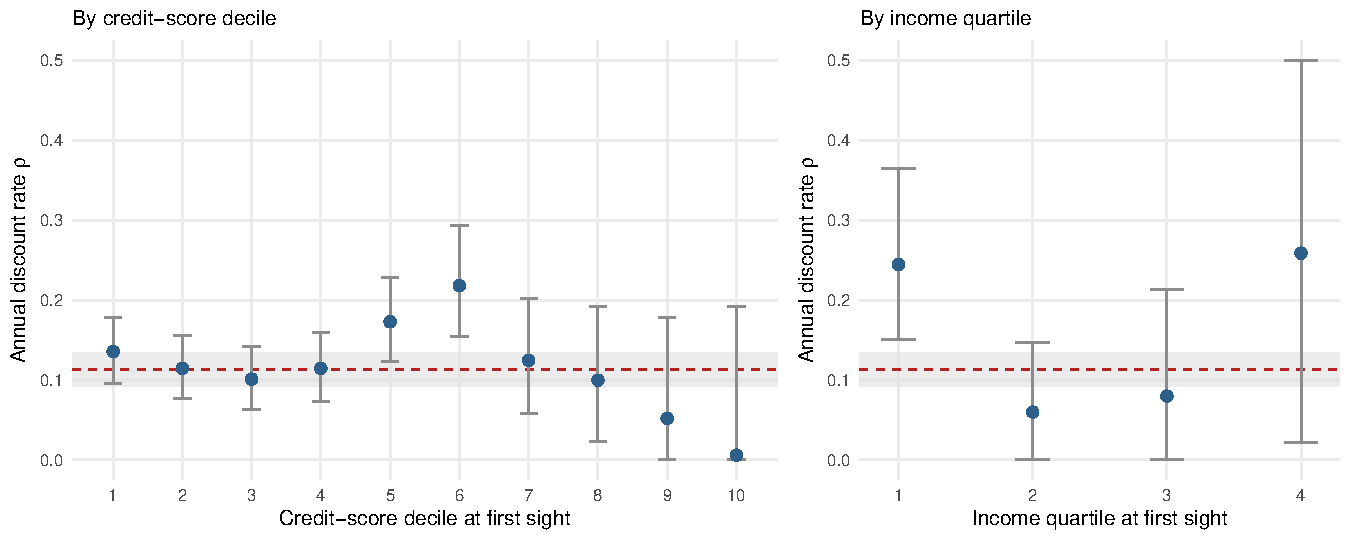
\includegraphics[width=0.9\textwidth]{figures/fig_rho_headline.pdf}
\caption{The rate. The within-borrower estimate of the annual discount rate by credit-score decile (left) and by income quartile (right), with 95 percent sets; the dashed line is the loan-weighted mean across deciles, $0.11$, and the band its 95 percent set (Section \ref{sec:rate_people}).}
\label{fig:rho_headline}
% replication: Code/local/within_reading.R, Code/exhibits/make_rho_headline_figure.R
\end{figure}

Three measured objects produce the number, and each has published counterparts, which is what a sufficient-statistics formula is for. The first is the response of default to the monthly payment: an elasticity of $0.45$ on 7 million auto loans within cells of lender, place, score and income, and $0.53$ within borrower on the 13.5 million borrowers with two or more auto loans in a ten-percent archive of credit files, 65 million loans. The second is the response of default to the contract's length at a fixed payment, which adds payments at the far end of the contract: $0.30$ within borrower at twenty-four months. The third is survival, the hazard at which a loan ends for a reason other than default, $0.19$ per year net of servicer transfers. The payment response has counterparts in every quasi-experiment that moved a mortgage or card payment by rule, and Table \ref{tab:benchmark} sets them beside the bureau's at the two margins the literature distinguishes, a payment change with the balance moving and one at a fixed balance. The far-payment response has counterparts in the two-arm experiments, to which Section \ref{sec:quasi} applies the same weights; a reader who prefers a published estimate of any input can substitute it and recompute the rate.

The credit bureau's contribution is the population and the designs. Auto loans reach the low end of the income and credit-score distributions, the households whose time preferences asset prices do not reveal and whom laboratory samples do not reach, and the panel records the score, income, lender and location of every loan. Four designs in these data identify a response without any assumption about who chooses which contract; three have their own subsections in Section \ref{sec:autodata}, and the fourth is in Appendix \ref{appendix:traits}. Within-borrower comparisons hold the person fixed and identify the payment and far-payment responses net of every stable trait; run group by group, they give the rate by score decile, income quartile and age (Section \ref{sec:rate_people}). State laws that bar lenders from pursuing the unpaid balance after repossession, and the recourse laws of mortgage states, identify the penalty channel of the term margin: where the balance cannot be pursued, a longer contract lowers early default by $0.36$ ($0.13$) less per unit of log length on small auto loans and by $3.9$ ($1.5$) less on mortgages, the cost of default rising with what is owed (Section \ref{sec:termmargin}). House-price movements across purchase cohorts within a zip code and quarter identify the walk-away response of mortgage default to negative equity, an elasticity of $-2.5$ that is stronger where the law bars recourse and convex in the shortfall (Section \ref{sec:equity}). And borrowers who move between areas identify the place's share of the geography of default, one tenth (Appendix \ref{appendix:traits}). A reader who accepts nothing else in the paper still has these.

The population step is not optional, and it rests on the designs. Simple fixed-effects regressions on every loan, benchmarked against the within-borrower estimates and the published quasi-experiments and interpreted as causal under a stated assumption, are what give heterogeneity at population scale with power (Section \ref{sec:identification}). What they show is that the heterogeneity in default across people is heterogeneity in exposure to the default margin, the density of borrowers at the threshold, and not in the rate: the payment elasticity is $0.41$ in the bottom income quartile and $0.86$ in the top, and the score-decile profile peaks near the median, while the within-borrower rate has no gradient in score or income (Section \ref{sec:heterogeneity}). The experiment that reports both of its arms by subgroup finds the same: the rate is the same above and below the median credit score and the median debt-to-income ratio (Section \ref{sec:quasi}). The one gradient in the bureau is age: borrowers aged 18 to 30 reveal a rate of $0.32$, with a set from $0.21$ to $0.48$, and every older group reveals zero.

Ahead of the exponential rate sits a premium on the payment due now. The marginal-utility ratio $\lambda$ of a repayer at a later date to the marginal defaulter today multiplies every future weight, and Section \ref{sec:results} shows that the present-bias parameter of \citet{laibson_golden_1997} and this ratio enter every default response as a product: in this class of models no comparison of a payment due now with payments due later separates them, and in that sense they are the same object. The paper measures the product from the one published comparison that holds the date fixed and varies the currency, the payment-relief and seizable-equity responses in \citet{indarte_moral_2023}, at $\lambda = 0.2$ as the level of a profile that declines with the horizon as the distress state mean-reverts, and states the assumption under which that ratio is the model's $\lambda$. The main text reports one exponential rate under time-consistent preferences with the premium as one measured number; the rate beyond the first payment is insensitive to it, and Appendix \ref{appendix:nonclassical} states what would identify its parts.

The estimates hold beliefs at their measured values. Survival enters every weight, so a borrower who expects to leave her loan sooner than the measured hazard would reveal a higher rate than she has; and a borrower who expects her income to recover weighs a later dollar less than the objective persistence of distress implies, which enters the premium. Neither belief is in the bureau's data. The 2022 Survey of Consumer Finances asks households what they expect of their own income, and Appendix \ref{appendix:beliefs} sizes both channels: constrained households expect a recovery of $0.11$ log points against $0.02$ for the unconstrained, the default-side correction to the rate is bounded by the group's default hazard, at most $0.06$ in the lowest score decile, and the expected recovery accounts for a first-year discount of 16 to 28 percent that sits inside the measured premium and is neither liquidity nor impatience.

Why must we look beyond asset prices? The Euler equation prices risk-free bonds using the discount factor of the \emph{marginal investor}, who is presumably wealthy and patient. The time preferences of the remaining households, the constrained, the hand-to-mouth, the borrowers, are not identified by these prices. Laboratory experiments offer an alternative, but the relevance of lab-elicited discount rates to real-world financial decisions is unclear, in part because behavior under small stakes may differ substantially from behavior under large stakes \citep{coller_eliciting_1999, harrison_estimating_2002, rabin_risk_2000}. The approach developed here uses real-stakes decisions at economically meaningful time horizons, observed at population scale.

The estimates have implications for credit policy and for public finance. For credit policy, the premium says that a dollar of relief on the payment due now prevents more default than a dollar of relief on a payment due later, by the factor $1/\lambda_s$, from $1.1$ for a payment due next month to about $3$ for one due five years out, and the two-arm experiments say the same only once their arms are classified by the sign of every month's payment change: a rescheduling that lowers payments now and adds them later is not relief, and its value to a borrower depends on the weights the formula assigns to the dates it moves payments between. For public finance, the estimate of $0.11$ is more than five times the two percent social discount rate the federal government applies, and \citet{hendren_unified_2020} show that the ranking of early-childhood against adult programs turns on rates in this range; for the households whose rate this is, the finding raises the value of programs with near-term payoffs relative to programs whose returns arrive decades later.

The paper proceeds as follows. Section \ref{sec:literature} states what the related literatures find and what this paper adds. Section \ref{sec:data} describes the panel. Section \ref{sec:suffstats} sets out the model, the sufficient-statistic results and their three provisos, the mapping from responses to a rate, and the published experiments. Section \ref{sec:autodata} applies the mapping to the credit-bureau panel, one design per subsection; Section \ref{sec:heterogeneity} reports exposure at population scale; Section \ref{sec:comparison} compares the estimates with prior work, Section \ref{sec:discussion} discusses what the rate and the premium capture, and Section \ref{sec:conclusion} concludes. The appendices prove the results, size the beliefs the estimates condition on, relax the classical preference restrictions, report every design in full, record the designs that do not identify the rate, and document the data and the replication of every exhibit.

% sections/literature.tex: Section 2: what each literature finds and what this paper adds.
\section{Related Literature}\label{sec:literature}

\paragraph{Discount rates from asset markets.} The standard approach to measuring time preferences uses the Euler equation to link the price of risk-free bonds to the discount factor of the marginal investor \citep{lustig_market_2005, bansal_risks_2004}. Calibrations of heterogeneous-agent models set $\delta \approx 0.96$ to match the capital-output ratio \citep{guvenen_reconciling_2006} or government bond yields, and \citet{di_tella_zero-beta_2024} construct a zero-beta rate from equity portfolios and estimate an average of 8.3 percent per year. These approaches identify the preferences of the marginal investor, presumably a wealthy and patient household, which may differ substantially from those of the typical household. This paper identifies the discount rate of the borrowing population, the majority of U.S.\ households, and finds it near the zero-beta rate and well above the calibrated factor.

\paragraph{Laboratory and field elicitations.} \citet{coller_eliciting_1999} elicit discount rates from students choosing between dated payments and find rates near 20 percent once the field interest rate is provided as a reference; \citet{harrison_estimating_2002} elicit 28 percent from a representative Danish sample over horizons of six months to three years. \citet{cohen_measuring_2020} survey 222 studies through 2016; the 112 that report a point estimate have a median of 22 percent per year and a mean of 26 percent, primarily from small samples with small stakes, and behavior under small stakes may differ from behavior under large stakes \citep{rabin_risk_2000}. The elicitations are over horizons of weeks to a few years, where a payment due now already differs from a payment due later by the premium this paper measures; the exponential rate this paper estimates over the contract horizon is a fraction of the elicited rates, and Section \ref{sec:comparison} states how the two segments of the schedule relate.

\paragraph{Default, payment relief and household debt.} \citet{ganong_liquidity_2020} use two regression discontinuities in the HAMP program and find that payment reductions prevent mortgage default far more effectively than principal reductions of equal cost. \citet{dobbie_targeted_2020} randomize the terms of debt-management plans and find that a write-down of the last payments lowers bankruptcy while an immediate payment reduction that adds payments later raises it. \citet{indarte_moral_2023} separates the cash-on-hand and moral-hazard channels of bankruptcy with adjustable-rate resets and exemption kinks and finds the cash-on-hand response an order of magnitude larger per dollar. Each of these designs is a payment path, and Section \ref{sec:quasi} applies the formula of this paper to their pairs: the first two identify a discount rate for the populations they treat, the third the marginal-utility ratio. \citet{ganong_consumer_2019} fit consumption during unemployment and find that about one third of consumers behave as impatient low-$\beta$ types, without a distribution of rates; this paper supplies the rate by group at population scale. The option-value view of default, in which the borrower who continues keeps the right to default later \citep{deng_mortgage_2000, campbell_model_2015}, is built into the model of Section \ref{sec:model} and is what prevents the decline of the payment response over the life of a loan from being a measure of the rate (Appendix \ref{appendix:mcliquidity}). \citet{athreya_persistence_2019} reproduce the persistence of financial distress within the person only with persistent heterogeneity in discount factors; this paper measures the person's share of the variance of default at a quarter and finds no gradient in the rate across the groups whose default rates differ most (Appendix \ref{appendix:traits}, Section \ref{sec:rate_people}).

\paragraph{Sufficient statistics.} The sufficient-statistics approach to welfare and policy analysis \citep{chetty_sufficient_2009} recovers policy-relevant parameters from a small number of estimable moments without specifying the full structure of the model. \citet{davila_exemptions_2020} applies it to household default: the optimal bankruptcy exemption depends on four measurable objects, among them the value households place on a marginal dollar in the bankruptcy state, which he recovers from consumption changes under an assumed utility function and an assumed annual discount factor of $0.94$. The discount function that paper assumes is the object this paper measures. The same ratio logic identifies a marginal-utility ratio at one date in \citet{chetty_moral_2008} and \citet{indarte_moral_2023}; this paper's increment is the ratio across dates, and Appendix \ref{appendix:priority} states the antecedent and the increment for each result.

\paragraph{Discount rates in public finance.} Governments publish declining discount-rate schedules for long horizons \citep{arrow_should_2014}, the U.S.\ government recently lowered its recommended social discount rate from 3 to 2 percent \citep{the_white_house_biden-harris_2023}, and \citet{hendren_unified_2020} show that the ranking of public investments turns on the rate, with adult programs dominating at high rates and early-childhood programs at low rates; \citet{demarzo_sovereign_2023} show that patient citizens are harmed when their government borrows excessively. This paper places the contract-horizon discount rate of borrowing households at $0.11$, above the two percent rate used in policy analyses and inside the set the rule-based experiments accept for distressed borrowers, with a further premium on the payment due now.

% sections/data.tex: Section 3. Counts: results/family_counts.csv, results/summary_stats_families.csv (E19), results/panel_windows_auto.csv.
\section{Data}\label{sec:data}

Three samples produce the estimates. The first is a one-percent consumer panel of U.S.\ credit files, observed semiannually from 2005 to 2009 and monthly from January 2010 to December 2025, which holds, across its six loan families (auto, first mortgage, home equity, personal installment, student and credit card), 67.2 million loans, more than 3.8 million borrowers and 5.8 million first ninety-day delinquencies; its 9.7 million auto loans, of which 7.6 million form the analysis sample, are the main panel. The second is a ten-percent trade archive, observed at 57 archive months from 2005 to April 2024 with a monthly score file from 2010, on which the within-borrower designs run: of its 15.5 million borrowers with two or more auto loans (83.5 million loans), the 13.5 million whose loans meet the contract restrictions below, 65 million loans. The third is the covariate-matched ten-percent extract, the loans of the one-percent consumers nested in the archive, which alone has age and income; the specification search of Appendix \ref{appendix:bridge}, the deficiency contrast and the term margin by score decile run on it (72,906 lifetime defaults). The population estimates run on the one-percent panel rather than the archive because the panel is monthly and records income and age on every loan, which the archive's quarterly snapshots do not; the archive's size is what the within-borrower designs need, since only a fraction of borrowers hold two auto loans with a default in the window. Appendix \ref{appendix:data} records the files, frequencies and restrictions of every exhibit.
\begin{table}[H]
\centering
\caption{Summary statistics by loan family}
\label{tab:summary_families}
\small
\resizebox{\textwidth}{!}{\begin{tabular}{lrrrrrr}
\toprule
 & Auto & Credit card & First mortgage & Student & Personal installment & Home equity \\
\midrule
\multicolumn{7}{l}{\emph{Panel A. Coverage: the one-percent consumer panel, 2005--2025}} \\
Loans (millions) & 9.66 & 34.20 & 6.12 & 8.61 & 8.08 & 0.53 \\
Borrowers (millions) & 2.20 & 3.81 & 1.46 & 0.94 & 1.53 & 0.28 \\
Lenders & 18,690 &  9,758 & 15,188 &  5,699 & 30,273 &  7,527 \\
Loans per borrower & 4.4 & 9.0 & 4.2 & 9.2 & 5.3 & 1.9 \\
Borrowers with two or more loans (percent) & 73.9 & 75.9 & 78.5 & 85.8 & 65.9 & 46.2 \\
Opening year, 10th to 90th percentile & 2003--2022 & 1995--2022 & 2001--2021 & 2001--2020 & 2002--2023 & 2002--2021 \\
Loans with a score and an income (percent) & 98.4 & 95.2 & 99.3 & 97.9 & 98.3 & 99.3 \\
\addlinespace
\multicolumn{7}{l}{\emph{Panel B. The contract at origination (medians)}} \\
Balance or limit (\$) &  19,089 &   1,215 & 169,000 &   3,744 &   2,791 &  36,366 \\
Scheduled monthly payment (\$) &   387 &    29 & 1,263 &    50 &   132 &   359 \\
Contract length (months) &  60 & revolving & 360 & 120 &  24 & 180 \\
Payment to monthly income & 0.114 & 0.010 & 0.290 & 0.021 & 0.053 & 0.088 \\
\addlinespace
\multicolumn{7}{l}{\emph{Panel C. The borrower at first sight}} \\
Credit score, median & 698 & 724 & 757 & 653 & 621 & 734 \\
Credit score, 10th to 90th percentile & 550--807 & 565--817 & 605--822 & 488--769 & 492--770 & 576--817 \\
Subprime, score below 620 (percent) & 25.0 & 19.7 & 12.0 & 38.2 & 49.6 & 16.4 \\
Modeled monthly income, median (\$) & 3,417 & 3,417 & 4,167 & 2,500 & 2,583 & 4,083 \\
Income below \$2,500 a month (percent) & 24.0 & 22.1 & 7.2 & 49.1 & 43.7 & 6.8 \\
Age, median & 44 & 48 & 47 & 31 & 46 & 47 \\
\addlinespace
\multicolumn{7}{l}{\emph{Panel D. Outcomes over the life of the loan}} \\
Ever 30 days past due (percent) & 12.5 & 13.9 & 12.1 & 17.1 & 11.3 & 13.9 \\
Ever 90 days past due (percent) & 3.5 & 9.3 & 6.4 & 15.9 & 5.8 & 8.9 \\
Charged off (percent) & 4.9 & 9.7 & 0.2 & 0.8 & 6.3 & 3.1 \\
90 days past due within 12 months (percent) & 0.6 & 1.9 & 0.2 & 0.5 & 1.9 & 0.3 \\
90 days past due within 24 months (percent) & 1.5 & 3.6 & 0.9 & 2.2 & 3.5 & 1.6 \\
Months to first 90 days past due, median & 28 & 32 & 55 & 61 & 13 & 49 \\
Charge-off amount over balance, median & 0.49 & 1.88 & 0.85 & 1.23 & 0.86 & 0.97 \\
\addlinespace
\multicolumn{7}{l}{\emph{Panel E. The ten-percent trade archive, 2005--2024 (within-borrower designs)}} \\
Loans (millions) & 89.0 &  & 58.2 &  & 73.4 & 4.9 \\
Borrowers (millions) & 21.1 &  & 14.1 &  & 14.4 & 2.6 \\
Borrowers with two or more loans (millions) & 15.5 &  & 11.1 &  & 9.4 & 1.2 \\
Their loans (millions) & 83.5 &  & 55.1 &  & 68.4 & 3.5 \\
Charged off (percent) & 4.1 &  & 0.1 &  & 5.7 & 2.5 \\
\bottomrule
\end{tabular}
}
\vspace{0.5em}
\begin{minipage}{0.96\textwidth}
\noindent \small \textit{Notes:} Panels A to D describe the one-percent consumer panel, semiannual from 2005 to 2009 and monthly from 2010 to 2025, with every loan of each family that the archive reports. A borrower is a hashed consumer identity; a lender is a hashed furnisher identity. The balance is the original balance for installment loans and the high credit at first sight for cards; the scheduled payment is the payment at first sight, for cards the minimum; a card's contract has no length. Modeled income is the bureau's estimate of monthly income at the quarter of first sight; the score is the bureau's risk score at the month of first sight; the row ``loans with a score and an income'' is the share of loans on which both covariates are recorded, the coverage of every exhibit that conditions on them. Delinquency and charge-off are the first occurrence over the loan's observed life; the twelve- and twenty-four-month rates condition on loans opened at least that long before the panel's last month and, for installment loans, on contracts of at least that length. The charge-off amount is divided by the balance at origination, so that it exceeds one where interest and fees were capitalized. Panel E describes the ten-percent trade archive, 57 snapshots from 2005 to 2024, on which the within-borrower designs run; cards and student loans have no extract from it.
\end{minipage}
% replication: Code/extract/E19_summary_stats.R, Code/exhibits/make_table1.R
\end{table}

The credit-bureau panel records every loan type a household holds, and the loan types differ in the three respects that matter for measuring a discount rate: the contract, which fixes the payment path and the horizon; the population, which fixes whose preferences the estimate describes; and the instruments, which fix what can be identified. Table \ref{tab:loan_types} in Appendix \ref{appendix:data} sets the loan types side by side. Auto loans and credit cards are the laboratories for the low end of the income distribution, and the auto-loan panel is the main sample for the estimates that follow. First mortgages are the laboratory for long horizons, up to thirty years, and the one whose instruments, house prices by origination cohort and state recourse law, are the strongest available; Section \ref{sec:equity} reports what they establish. Student loans have the one payment fixed by statute, the resumption of October 2023; Appendix \ref{appendix:timing} reports that design and the adjustable-rate resets of first mortgages in full. The panel is a consumer credit panel drawn from the files of a national credit bureau, one of the panels surveyed by \citet{gibbs_consumer_2025}, and every measure follows their guidance except where Appendix \ref{appendix:data} states otherwise.

\paragraph{The auto-loan panel.} Auto loans offer an attractive empirical setting: maturities vary substantially, payments are highly salient, and auto loans are one of the most common forms of installment credit, with wide participation across the income distribution. The analysis sample restricts the panel's 9.7 million auto loans to contracts of 12 to 96 months with a positive scheduled payment, a score and an income, and an identified lender: 7.6 million loans at 15,532 lenders. The typical repayment horizon is five years, and the three most popular maturities, 36, 60 and 72 months, account for over half of the loans; origination volumes are steady from 2010 onward (Figure \ref{fig:origination_volume}, Appendix \ref{appendix:figures}). Table \ref{tab:summary_families} summarizes the key variables by family, Table \ref{tab:loan_summary} in Appendix \ref{appendix:procedures} the auto panel's quartiles, and Appendix \ref{appendix:procedures} the construction.

% sections/theory.tex: Section 4: the model, the sufficient-statistic results with the two provisos, and the mapping from
% responses to a rate. Proofs in Appendix appendix:multiperiod; the two-period derivation in Appendix appendix:proofs.
\section{A Sufficient Statistics Approach to Measuring Discount Rates}\label{sec:suffstats}

\paragraph{Notation.} Throughout the paper $\delta$ is the exponential discount factor, $\beta$ the present-bias parameter of the quasi-hyperbolic extension (Appendix \ref{appendix:nonclassical}), which equals one under exponential discounting, and $\rho$ the continuous annual discount rate ($\delta = e^{-\rho}$ over a year and $e^{-\rho/12}$ over a month); the persistence of income in the calibration appendix is $\varrho$. $D(k)$ is the discount function, the weight on utility $k$ periods ahead, with $D(0) = 1$ and $D(k) = \delta^k$ under exponential discounting. $\lambda$ is the marginal-utility ratio of equation \eqref{eq:twoperiod}: the expected marginal utility of a dollar to a borrower who is still repaying at a later date, divided by the marginal utility of a dollar to the borrower who is exactly indifferent between paying and defaulting today. $\gamma$ is relative risk aversion; regression coefficients have subscripts ($\gamma_m$, $\gamma_T$); the loss-aversion coefficient of the reference-dependent extension is $\lambda_L$ and $\theta_s$ the attention weight of the same extensions (Appendix \ref{appendix:nonclassical}). $\sigma$ is the default penalty flow of the $T$-period model, $\kappa_B$ the scale of the penalty that rises with the balance owed, and $h$ the annual hazard at which a loan ends before maturity for a reason other than default. No functional form for utility enters the identifying identity; functional forms are used in two places only, the calibration that makes $\lambda$ a function of a group's default rate (Appendix \ref{appendix:mucorrection}) and the simulated model of Appendix \ref{appendix:mcliquidity} that analyzes how sensitive the rate is to the option to default later.

What can we learn about households' impatience from their default decisions? The rate at which a household borrows reveals a composite of its discount rate, its subjective probability of repaying and the premium on a present dollar, and does not point-identify the discount factor (Appendix \ref{appendix:beliefs}). Default decisions encode a richer intertemporal tradeoff. I show that in a simple endogenous default model with separable utility, the causal effects on default of changes in repayment obligations at two different time horizons are sufficient to point-identify the discount factor $\delta$ between those two horizons, up to a single marginal-utility ratio, which the experiments of Section \ref{sec:quasi} measure and Appendix \ref{appendix:mucorrection} bounds from the persistence of the marginal borrower's economic state. No functional form for the utility function is required beyond strict concavity and monotonicity for the identifying identity itself.

The economic intuition is as follows. An impatient borrower responds to the payment due now and little to the same dollars due later: a higher payment this month raises the temptation to default, and a higher payment a year from now barely moves it. A patient borrower responds to a dollar due later nearly as she responds to a dollar due now. The ratio of the response to a later payment to the response to the current one reveals the weight the borrower places on the future relative to the present. The contract's length is not that comparison. A longer contract at a fixed payment adds payments at the far end, but it also raises the balance the lender can pursue after default and the number of months in which a default can occur (Proposition \ref{prop:termmargin}).

Can default choices reveal time preferences? The theory's answer is yes, with two provisos. First, the payment due now has a premium over every later payment, the marginal-utility ratio $\lambda$, which multiplies the discount function; no comparison of a payment due now with payments due later, in any experiment, separates that premium from present bias, because the two enter every default response as a product (Theorem \ref{thm:betalambda}). A comparison of a liquid with an illiquid dollar at one date does separate them (Corollary \ref{cor:separate}); the paper measures the premium from one such comparison, Indarte's, and Section \ref{sec:quasi} reports how much the rate moves with it. Second, beliefs enter the same weights as a product with the discount function: the borrower's own probability of still facing a payment, and her expectation of her income at the date the payment is due (Proposition \ref{prop:beliefs}). The discount function is identified with beliefs fixed; the panel fixes survival at its measured value, and Appendix \ref{appendix:beliefs} sizes both beliefs in the Survey of Consumer Finances, which is what that survey is for in this paper. The contract's length, the bureau's own source of variation in far payments, is not a payment at a date, and what it measures is stated where it is used (Section \ref{sec:identification}, Proposition \ref{prop:termmargin}). Variation that moves a payment at a known date with the balance fixed, the rule-based experiments, identifies a rate without a model of the penalty; run over outcome windows of years at horizons of four to twenty-six years, the published experiments accept the bureau's estimate and reject little else, for the reason Section \ref{sec:mapping} gives, and they check the sign and the horizon of the far-payment response rather than its level. Section \ref{sec:model} sets out the model, Section \ref{sec:results} states the identity and the two results, with proofs in Appendix \ref{appendix:multiperiod}, Section \ref{sec:mapping} maps default responses to a rate, and Section \ref{sec:quasi} applies the mapping to the rule-based experiments.

\subsection{The Model}\label{sec:model}

\paragraph{Two periods.} Payments are due at two dates, $m$ now and $L - m$ later, with $L = 2m$ in the base case. Income $y_1$ is drawn from a distribution $F$ and is net of the household's non-discretionary expenses throughout the paper, so that a shock to $y$ is an expense shock as much as an earnings shock \citep{fulford_expense_2024}; no distributional assumption is needed. Default costs a punishment $\sigma$, which stands for credit-market exclusion, stigma and garnishment \citep{indarte_moral_2023}, and the borrower has strictly increasing, strictly concave utility, additive across the two dates with discount factor $\delta$. The date-2 threshold $y_2^*$ equates the utility of paying with the utility of defaulting, and the date-1 threshold $y_1^*$ equates the value of paying now, $u(y_1 - m) + \delta\,\mathbb{E}[V_2^P]$, with the value of defaulting now, $u(y_1) + \delta\,\mathbb{E}[V_2^N]$, where $V_2^P$ and $V_2^N$ are the date-2 values after paying and after defaulting (Appendix \ref{appendix:proofs} states the problem in full):
\begin{equation}\label{eq:threshold1}
u(y_2^* - (L - m)) = u(y_2^*) - \sigma, \qquad u(y_1^* - m) + \delta\,\mathbb{E}[V_2^P] = u(y_1^*) + \delta\,\mathbb{E}[V_2^N].
\end{equation}
Default probabilities are $p_t = F(y_t^*)$, and implicit differentiation of the date-1 condition gives the two responses that everything else is built on (Appendix \ref{appendix:proofs}):
\begin{equation}\label{eq:sensitivities}
\frac{\partial p_1}{\partial L} = f(y_1^*)\,\delta\,(1 - p_2)\,\frac{\mathbb{E}\left[u'(C_2^P) \mid y_2 > y_2^*\right]}{u'(y_1^* - m) - u'(y_1^*)}, \qquad
\frac{\partial p_1}{\partial m} = f(y_1^*)\,\frac{u'(y_1^* - m)}{u'(y_1^* - m) - u'(y_1^*)} - \frac{\partial p_1}{\partial L},
\end{equation}
with $C_2^P = y_2 - (L - m)$ the consumption of a date-2 repayer. A higher far payment $L$ lowers the continuation value of repaying and raises default; a higher current payment $m$ raises the marginal utility of consuming today and the gain from not paying. The ratio of the two responses eliminates the density at the default margin and the scale of utility. Write $A \equiv \partial p_1/\partial L$ for the response to the far payment and $B \equiv (1 - p_2)\,\partial p_1/\partial m$ for the response to the current payment, scaled by the probability of reaching the second date. Then
\begin{equation}\label{eq:twoperiod}
\frac{A}{A + B} \;=\; \delta\,\lambda, \qquad
\lambda \;\equiv\; \frac{\mathbb{E}\left[u'(C_2^P) \mid y_2 > y_2^*,\, y_1 = y_1^*\right]}{u'(y_1^* - m)}.
\end{equation}
The left side is the share of the total default response that the far payment accounts for. The right side is the discount factor times the \emph{marginal-utility ratio} $\lambda$, defined in the same display: the average marginal utility of future repayers conditional on standing at today's default margin, over the marginal utility of the marginal defaulter herself. With concave utility they differ, and for a liquidity-constrained borrower the ratio is well below one. If default decisions are entirely forward-looking, the far payment accounts for the whole response and $\delta\lambda = 1$; if they are entirely myopic, $\delta\lambda = 0$. The two-period model offers one future date and identifies the product $\delta\lambda$, not its factors; the $T$-period model below offers many, and two future dates $t_1, t_2 \ge 2$ identify $\delta$ alone:
\begin{equation}\label{eq:twofuture}
\frac{\partial p_1/\partial m_{t_2}}{\partial p_1/\partial m_{t_1}} \;=\; \delta^{\,t_2 - t_1}\,\frac{Q_{t_2}}{Q_{t_1}},
\end{equation}
where $Q_t$ is the probability of still facing the payment at $t$, when the marginal-utility ratio is the same at the two dates; in general the ratio has the further factor $\lambda_{t_2}/\lambda_{t_1}$, which the profile stated below supplies. This is the comparative static the abstract names, and the two-arm experiments of Section \ref{sec:quasi} supply it. The paper treats $\lambda$ as a measured input rather than an assumption: Section \ref{sec:quasi} measures it from the pair of responses in \citet{indarte_moral_2023}, to a dollar of payment relief within the year and to a dollar of seizable wealth at the filing date, which compares a liquid dollar with an illiquid one for a household at the bankruptcy margin, at $\lambda \approx 0.2$; Appendix \ref{appendix:mucorrection} bounds it from the other side, from the measured persistence of the distress state (Table \ref{tab:mucorrection}). The comparisons of payment elasticities in Section \ref{sec:heterogeneity} do not involve $\lambda$, and the rate comparisons of Section \ref{sec:rate_people} use each group's own profile; the level of the rate depends on how the premium is spread over the later payments, and Sections \ref{sec:quasi} and \ref{sec:rate_people} report the sensitivity.

\paragraph{$T$ periods.} The two-period structure is a special case of a general model. A contract specifies payments $m_t > 0$ at dates $t = 1, \dots, T$, with balance $L = \sum_t m_t$; for an annuity, $m_t = m$ at every date. Income $y_t$ is drawn i.i.d.\ from $F$ with continuous density $f$ and full support on $(0,\infty)$; the results below go through with Markov income (Remark \ref{appendix:continuous} in Appendix \ref{appendix:multiperiod}); income is net of non-discretionary expenses throughout. Consumption equals income net of any payment, utility $u$ is strictly increasing, strictly concave, and satisfies $u(0^+) = -\infty$ (e.g.\ CRRA with $\gamma \ge 1$). Default is absorbing: a borrower who defaults at $t$ consumes her income thereafter and incurs a punishment flow $\sigma > 0$ in each period $s \in \{t, \dots, T\}$; Section \ref{sec:results} adds a component of the punishment that scales with the balance owed. All agents are identical after $T$, so post-$T$ values are normalized to zero. The borrower discounts utility $k$ periods ahead by the discount function $D(k)$, exponential, $D(k) = \delta^k$, unless stated otherwise. A loan may also end before the next payment for a reason other than default, with monthly probability $1 - e^{-h/12}$ at the annual exit hazard $h$: the borrower sells or trades in the vehicle and pays the loan off, refinances it, or the loan is transferred to another servicer, which ends it under one furnisher's key and restarts it under another's (Appendix \ref{appendix:data}). The results are stated with $Q_s$ the probability that the borrower still faces the payment at $s$, which the exits lower, and Section \ref{sec:mapping} states how it is measured.

Let $W_t = \sum_{k=0}^{T-t}\delta^k(\mathbb{E}u(y) - \sigma)$ denote the defaulted value and
\begin{equation}\label{eq:bellmanT}
V_t(y) = \max\big\{\, u(y - m_t) + \delta \mathbb{E}V_{t+1},\;\; u(y) - \sigma + \delta W_{t+1} \,\big\}, \qquad V_{T+1} \equiv 0,
\end{equation}
the value of good standing. Write the surplus from staying as $\Delta_t(y) = K_t - g_t(y)$, where $g_t(y) \equiv u(y) - u(y-m_t) > 0$ is the utility cost of paying, strictly decreasing on $(m_t,\infty)$, and $K_t \equiv \sigma + \delta(\mathbb{E}V_{t+1} - W_{t+1})$ is the value of standing. The borrower defaults iff $y < y_t^* = g_t^{-1}(K_t)$, so that $p_t = F(y_t^*)$, and $Q_s = \prod_{k=2}^{s}(1-p_k)$ is the probability of good standing through date $s$. Default is an optimal stopping problem: a borrower who stays today is not committing to repay the remaining $T-t$ installments but buys one period of good standing plus the option to reconsider, and Proposition \ref{prop:interiorT} in Appendix \ref{appendix:multiperiod} shows that, for this reason, every default probability is strictly interior at any horizon $T$ and any payment schedule, provided the punishment has a flow component. The same appendix characterizes the two modeling choices that instead produce degenerate corner probabilities, comparing default against committed repayment of all remaining installments (Lemma \ref{lem:committedT}) and letting the punishment vanish at maturity.

\paragraph{The marginal-utility ratio with many dates.} With many dates the ratio is date-specific: $\lambda_s = \mathbb{E}[u'(y - m_s) \mid y > y_s^*]/u'(y_1^* - m_1)$ compares the repayers' expected marginal utility at $s$ with the marginal defaulter's today. With income independent across months and a constant payment, the repayers' expected marginal utility is the same at every future date, so $\lambda_s = \lambda$ for all $s \ge 2$: the two-period object applied to every later payment, the convention under which Indarte's pair is mapped to $\lambda$. With a persistent income state the profile declines: a borrower at the default margin today is likely still constrained next month, so $\lambda_2$ is near one, and $\lambda_s$ falls toward the independent-income value as the distress state mean-reverts. The paper maps every ratio through the profile, because the profile is the measured object: the persistence of the distress state is measured in the panel, $0.52$ per year (Appendix \ref{appendix:measuredrho}), and the curvature that turns persistence into a profile is the one that passes the constant-income limit through Indarte's value. Under that persistence the calibration that gives $\lambda(p) = 0.34$ for the pooled auto population as a constant gives $\lambda_2 = 0.89$, $\lambda_{12} = 0.59$ and $\lambda_{60} = 0.35$ (equation \eqref{eq:lambda_p}). A declining profile gives the near payments more weight than a constant assigns them, so that for a given ratio of the far-payment response to the payment response a constant premium returns a rate above the profile's; Section \ref{sec:rate_people} reports the constant-premium rate beside the estimate as the sensitivity.

\subsection{Sufficient-Statistic Results}\label{sec:results}

Fix the schedule $(m_1,\dots,m_T)$ and let $\Delta u_1' \equiv u'(y_1^* - m_1) - u'(y_1^*) > 0$ denote the gap in marginal utility across the two branches at the date-1 threshold. Appendix \ref{appendix:multiperiod} proves each result of this subsection.

\begin{proposition}[Sensitivities to the payment schedule]\label{prop:sensT}
Under exponential discounting,
\begin{align}
\frac{\partial p_1}{\partial m_1} &= f(y_1^*)\,\frac{u'(y_1^* - m_1)}{\Delta u_1'}, \label{eq:sens1T}\\
\frac{\partial p_1}{\partial m_s} &= f(y_1^*)\,\delta^{s-1} Q_s\, \frac{\mathbb{E}[u'(y - m_s) \mid y > y_s^*]}{\Delta u_1'}, \qquad s \ge 2, \label{eq:senssT}
\end{align}
where $Q_s = \prod_{k=2}^{s}(1-p_k)$ is the probability of good standing through date $s$.
\end{proposition}

With $T = 2$, $m_1 = m$, and $m_2 = L - m$, equations \eqref{eq:sens1T}--\eqref{eq:senssT} reduce exactly to equation \eqref{eq:sensitivities}. The ratio of the response to a later payment to the response to the current one cancels the density at the default margin and the scale of utility. Under a general discount function $D$, with either exponential discounting or a naive borrower, the same argument gives
\begin{equation}\label{eq:curveT}
\frac{\partial p_1/\partial m_s}{\partial p_1/\partial m_1} = D(s-1)\, Q_s\, \frac{\mathbb{E}[u'(y-m_s) \mid y > y_s^*]}{u'(y_1^* - m_1)}, \qquad s = 1, \dots, T.
\end{equation}
The right side is the weight a payment due at $s$ has relative to the payment due now,
\begin{equation}\label{eq:weights}
w_1 = 1, \qquad w_s = D(s-1)\,Q_s\,\lambda_s, \qquad \lambda_s \equiv \frac{\mathbb{E}[u'(y - m_s) \mid y > y_s^*]}{u'(y_1^* - m_1)}, \qquad s \ge 2,
\end{equation}
the product of the discount function, the probability of still facing the payment, and the marginal utility of a dollar at $s$ relative to a dollar at today's default threshold. In logs the weight is the Euler equation's decomposition of the rate a household demands to defer a dollar: $-\log w_s = \rho\,(s-1)/12 - \log\lambda_s - \log Q_s$, pure impatience plus a consumption-smoothing term plus survival. A household at the default margin may weigh a later dollar lightly not because it is impatient but because it expects its own circumstances to improve, the borrower who sees herself as temporarily embarrassed; that expectation is the consumption-smoothing term, and it is $\lambda_s$, measured, and not $\rho$. The identification results below are statements about which comparisons move which term. A treatment that changes the payment path by $\{X_s\}$ therefore moves default by $\phi\sum_s w_s X_s$ to first order, with the scale $\phi = f(y_1^*)\,u'(y_1^* - m_1)/\Delta u_1'$ common to every date, and the ratio of two treatments' effects in the same population is the ratio of their weighted sums, in which $\phi$ cancels. This is the identity every estimate in the paper is built on; it identifies $D$ given survival and the marginal-utility ratio. Every outcome in the paper is measured within a window, default within $K$ months, and a window aggregates decisions: a loan that defaults in month $t$ of the window did so at a decision at which the payment due now was the $t$-th and the far payments stood $T - t$ months ahead. With $\omega_t$ the share of the window's defaults that occur in month $t$, measured in the panel, the response of default within the window to a treatment is $\phi\sum_{t \le K}\omega_t\sum_{s \ge t} w^{(t)}_{s-t+1} X_s$, with $w^{(t)}$ the weights of equation \eqref{eq:weights} taken from the decision date $t$. For an annuity of $T$ payments under exponential discounting and survival at the exit hazard $h$, the elasticity of default within $K$ months to the contract's length at a fixed payment, which adds a payment at the end of the contract, over its elasticity to the payment, which moves every payment, is to first order
\begin{equation}\label{eq:window}
R_K \;=\; \frac{\sum_{t \le K}\omega_t\, T\, w_{T-t+1}}{\sum_{t \le K}\omega_t \sum_{k=1}^{T-t+1} w_k}, \qquad w_1 = 1, \qquad w_k = \lambda_k\,e^{-(\rho + h)(k-1)/12}, \quad k \ge 2,
\end{equation}
the formula through which Section \ref{sec:rate_people} maps the bureau's within-borrower ratios to a rate and Section \ref{sec:quasi} tests the experiments' pairs, each with its own window and event timing in place of $\omega_t$. With $K = 1$ and a constant $\lambda_k = \lambda$ it is the date-1 formula $R = T w_T/\sum_{s \le T} w_s$ of a decision at origination, the special case without a balance-scaled penalty of equation \eqref{eq:Rs} in Appendix \ref{appendix:formula}. The date-1 formula assigns every default in a two-year window to a decision at origination, where the far payment is farthest and its weight smallest; a default in month 24 was decided when the far payment stood 37 months ahead rather than 60, and the date-1 formula reads the same ratio as a lower rate than the window's decisions reveal.

The two provisos follow from equation \eqref{eq:curveT}. The first concerns the weight on the payment due now.

\begin{proposition}[The present-payment premium]\label{prop:premium}
In the model of Proposition \ref{prop:sensT}, the weight on the payment due now relative to the payment due at $s \ge 2$ is
\[
\frac{\partial p_1/\partial m_1}{\partial p_1/\partial m_s} \;=\; \frac{1}{D(s-1)\,Q_s\,\lambda_s},
\]
with $\lambda_s$ the marginal-utility ratio of equation \eqref{eq:weights}, and $\lambda_s < 1$ whenever the marginal defaulter's consumption at date 1, $y_1^* - m_1$, is below the repayers' expected consumption at date $s$. The present payment therefore has a premium over every later payment that is separate from, and multiplies, the discount function, and it is bounded away from one for a liquidity-constrained marginal defaulter however patient she is.
\end{proposition}

\begin{theorem}[Present bias and the premium are not separable]\label{thm:betalambda}
Let $D(k) = \beta\delta^k$ for $k \ge 1$ with $D(0) = 1$, and let $\lambda_s = \lambda$ for all $s \ge 2$. Then every ratio of default responses to payments at dates $s, s' \ge 1$ depends on $(\beta, \lambda)$ only through the product $\beta\lambda$: for $s \ge 2$, $(\partial p_1/\partial m_s)/(\partial p_1/\partial m_1) = \beta\lambda\,\delta^{s-1} Q_s$, and for $s, s' \ge 2$ the ratio is $\delta^{s-s'} Q_s/Q_{s'}$. Consequently no set of perturbations of the payment schedule, however rich, and no experiment that moves payments due now against payments due later, identifies $\beta$ and $\lambda$ separately; $\delta$ and the product $\beta\lambda$ are identified, and $\beta = 1$ is observationally equivalent to any $(\beta, \lambda')$ with $\beta\lambda' = \lambda$.
\end{theorem}

\noindent The present-bias parameter of \citet{laibson_golden_1997} and the marginal-utility ratio that \citet{indarte_moral_2023} conditions on distress are, in every model of this class, the same object as far as default responses to payment timing are concerned: they enter every such response only as the product $\beta\lambda$. A study that attributes the whole premium to present bias measures its $\beta$ as this paper's $\lambda$, and one that attributes it wholly to liquidity measures its $\lambda$ as the other's $\beta$.

\begin{corollary}[What separates them]\label{cor:separate}
$\lambda$ is identified by a comparison at one date between a dollar valued at the marginal defaulter's marginal utility and a dollar valued at a repayer's: a change in liquid resources at the decision date against a change in the value of default at the same date, such as the payment-reduction and seizable-equity responses of \citet{indarte_moral_2023}, whose ratio does not depend on $D$ except through the months over which the relief is spread. The ratio equals $\lambda$ under the assumption that the marginal utility of a dollar of protected, illiquid wealth to a household at the default margin is the marginal utility of a repayer's later dollar, which is the sense in which both are the price of liquidity at the margin. Given $\lambda$, the product identifies $\beta$. Absent such a pair, a reader may attribute the whole premium to present bias or the whole of it to liquidity; the data cannot adjudicate, and the paper reports the product as one measured number.
\end{corollary}

The second proviso concerns the survival weight.

\begin{proposition}[Beliefs enter the weights multiplicatively]\label{prop:beliefs}
Let the borrower's subjective probability of remaining in good standing through $s$ be $\tilde Q_s$, possibly different from the objective $Q_s$. Then \eqref{eq:curveT} holds with $\tilde Q_s$ in place of $Q_s$, and the object identified from default responses with objective survival substituted is $D(s-1)\,\tilde Q_s/Q_s$. The discount function is identified only with beliefs fixed, and fixing them at the objective survival measured in the panel loads any optimism or pessimism about survival onto $D$.
\end{proposition}

\noindent This is the non-identification of \citet{manski_measuring_2004}, that choices reveal preferences only jointly with beliefs, in the setting of default responses: subjective and objective survival cannot be told apart from the responses alone. The paper's response is to measure $Q_s$ directly, from the exit, default and cure hazards of the panel, to state every discount rate as the rate that rationalizes the observed responses under those beliefs, and to size in survey data how far the beliefs of constrained households depart from the objective values (Appendix \ref{appendix:beliefs}). The expectation of income at the date a payment is due enters the same way, through $\lambda_s$.

Three further results of Appendix \ref{appendix:multiperiod} are used later. Proposition \ref{prop:curveT} states what an experiment must do to identify the whole discount curve: perturb each payment separately within one population, and with three or more future horizons the exponential form is testable; Remark \ref{rem:experimentsT} states why comparisons across borrowers who selected into different contract lengths do not qualify. Remark \ref{rem:option} states that a borrower who continues keeps the option to default later, so the far payments enter her decision only with the weight of the states in which she will still be paying them; for that reason the decline of the payment response with loan age is compared with the stopping model's own decline rather than mapped to a rate (Section \ref{sec:mainresults}, Appendix \ref{appendix:mcliquidity}).

\subsection{From Default Responses to a Discount Rate}\label{sec:mapping}

Proposition \ref{prop:sensT} gives the default response to a change in the payment at date $s$ as the product of a common scale $\phi$ and the date-specific weight of equation \eqref{eq:weights}, and the ratio of two treatments' effects in the same population cancels the scale. The ratio identifies the discount function only with the other two weights, survival and the marginal-utility ratio, supplied, and this subsection states how each is.

Survival is measured. For a borrower deciding today, $Q_s$ is the probability of being current at $s$, which falls with the default hazard and the payoff hazard. In the model default is absorbing, the terminal event that ends the contract; in the data a delinquency spell that begins does not always end the contract, since one fifth of delinquent auto trades return to current within a four-month interval (Appendix \ref{appendix:measuredrho}). The cure rate therefore scales the delinquency hazard to the hazard of the terminal event the model describes. For the experiments of Section \ref{sec:quasi} the default and payoff hazards are each study's own, and the cure rate is the one bureau input; for the auto-loan panel Section \ref{sec:autodata} measures the default and payoff hazards directly.

The marginal-utility weight $\lambda_s$ is the ratio of the average repayer's marginal utility at $s$ to that of the marginal defaulter today, below one when the marginal defaulter is liquidity-constrained (Proposition \ref{prop:premium}), and it is a profile over the horizon, from one source. Its level is measured: $0.2$ is the value that the comparison of a payment reduction with a change in seizable home equity in \citet{indarte_moral_2023} identifies under the assumption of Corollary \ref{cor:separate}, at her population's default rate and payment share (Section \ref{sec:quasi}). Its dependence on the group is the function $\lambda(p)$ of the default rate, the constant-relative-risk-aversion calibration of Appendix \ref{appendix:mucorrection} that passes through Indarte's value: a group whose default is rare has its marginal defaulter far in the lower tail of income, where marginal utility is steep, and therefore a smaller weight. Its shape over the horizon is the profile of Section \ref{sec:model} at the persistence of the distress state measured in the panel, equation \eqref{eq:lambda_p}: across the bureau's groups $\lambda_2$ is $0.88$ to $0.89$ and $\lambda_{60}$ runs from $0.26$ to $0.40$, and for each experiment's population the profile is taken at the study's own baseline rate and payment share. Sections \ref{sec:quasi} and \ref{sec:rate_people} report how far the estimates move under a constant premium of $0.2$ or $0.5$ in place of the profile.

For the credit-bureau data there is one more step. The term margin contains the penalty channel of Proposition \ref{prop:termmargin}, whose weight on a distant payment is $\kappa_B(1+r)^{-(s-1)}$ at the contract rate $r$, and, across borrowers, selection into contract length. Within borrower, selection is removed by design; the estimate of Section \ref{sec:rate_people} is taken at twenty-four months, where the penalty channel, which dominates within the first year, has decayed with the balance, and the deficiency contrast of Section \ref{sec:termmargin} measures the size of that channel. Across borrowers the two channels are adjusted for one at a time in Appendix \ref{appendix:ladder}, which reproduces the within-borrower estimate with less precision. The decline of the payment response with loan age is compared with the stopping model's own decline rather than mapped to a rate, for the reason Remark \ref{rem:option} gives. The rule-based experiments, which move payments by rule and hold the balance's legal treatment fixed, identify a rate without a model of the penalty; the next paragraph states why, at the windows and horizons at which they were run, they check the sign and the horizon of the far-payment response and not its level.

Figure \ref{fig:design_map} in Appendix \ref{appendix:figures} shows how the designs of the paper, each in its own section, supply the inputs of the formula and what each output rests on.

\paragraph{The horizon at which a rate can be estimated.} The weights say where in a contract a rate can be estimated and where it cannot. A response to a payment at horizon $s$ estimates the weight $w_s = \lambda e^{-(\rho + h)(s-1)/12}$ with some sampling error, and the rate is obtained from the weight's dependence on $\rho$. The delta method gives the standard error of the rate as the standard error of the response over $|\partial w_s/\partial \rho| = (s-1) w_s/12$, so that, for a response measured with a given absolute precision, the standard error of $\rho$ is proportional to $e^{(\rho + h)(s-1)/12}/(s-1)$. Compounding makes a far weight more sensitive to the rate, in proportion to the horizon; discounting and survival make the weight itself, and with it the response the data contain, smaller, exponentially in the horizon. The standard error is smallest at a horizon of $1/(\rho + h)$ years, $3.3$ years at the rate and exit hazard of the auto panel, and rises without bound on either side: at 26 years, the horizon of the Ganong--Noel forgiveness arm, $134$ times less precisely (Figure \ref{fig:horizon_power}, left). The same calculation for the bureau's term-to-payment ratio of equation \eqref{eq:window}, at the precision the within-borrower design attains, gives the smallest difference in the rate that a contract of each length can detect at the 95 percent level: $0.05$ for a five-year contract in one score decile, $0.06$ for a ten-year contract, and $2.4$ for a thirty-year mortgage (Figure \ref{fig:horizon_power}, right). A window adds a second loss. An outcome measured over five years, as the Dobbie--Song pair's is, averages the far payment's weight over decisions spread across sixty months, at some of which the forgiven payments are a year away and at others four, and the averaged weight moves with the rate more slowly than any one decision's does: aggregated over its own window, the pair accepts every rate from zero to $1.2$ at the five percent level (Section \ref{sec:quasi}). No design in these data, and no published experiment, estimates a long-run rate: the paper's object is the rate over the horizon of an installment contract, the auto loan sits where that rate is best measured, and that is why the level is the bureau's and the experiments are the check.

\begin{figure}[ht]
\centering
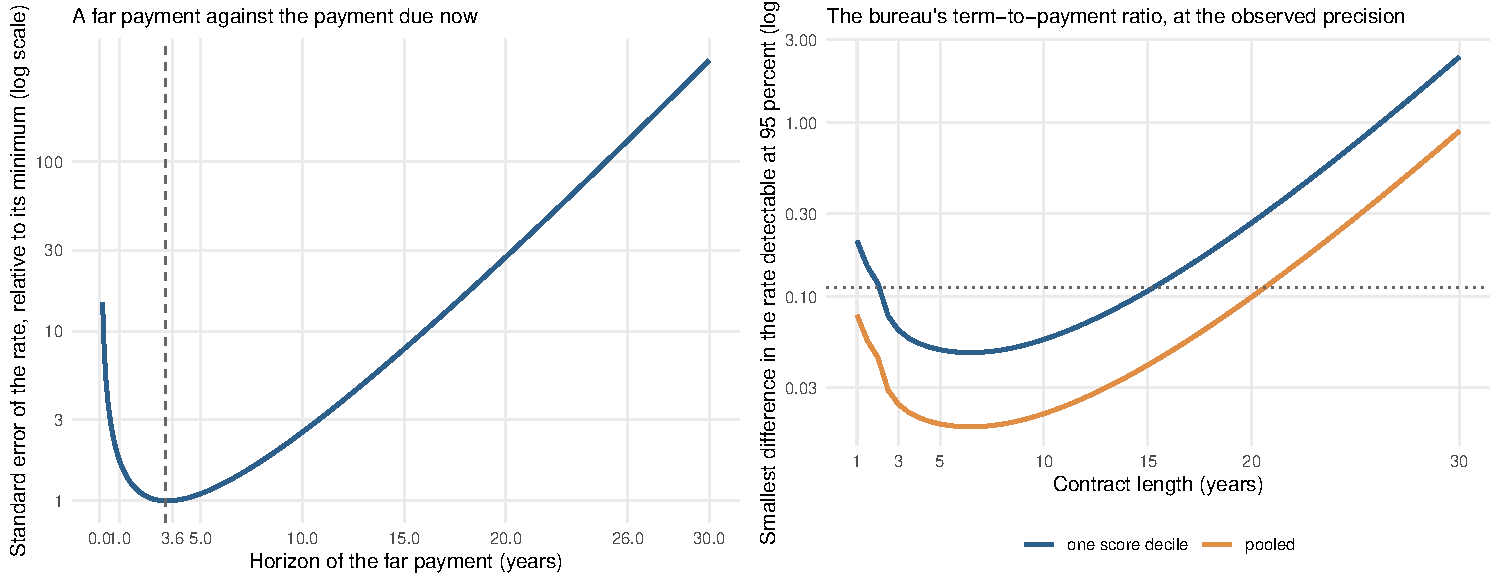
\includegraphics[width=\textwidth]{figures/fig_horizon_power.pdf}
\caption{The precision of the rate by horizon. Left: the standard error of the rate obtained from a single far payment against the payment due now, relative to its minimum, by the horizon of the far payment; the dashed line is $1/(\rho + h)$ years at $\rho = 0.11$ and $h = 0.19$. Right: the smallest difference in the rate detectable at the 95 percent level from the term-to-payment ratio of an annuity, by contract length, at the standard error of the ratio in the pooled within-borrower sample and in one score decile, through equation \eqref{eq:window}; the dotted line is the estimate, $0.11$.}
\label{fig:horizon_power}
% replication: Code/local/horizon_power.R; results/horizon_power.csv, results/rho_within_readings.csv
\end{figure}


% sections/external_experiments.tex - Section 4.4: the rule-based experiments as payment-path treatments. Ledger:
% external/experiments_paths.csv, external/experiments_estimates.csv; readings: Code/local/experiments_ledger.R,
% Code/local/experiments_rho_subgroups.R. Every number under the window aggregation of eq:window at the marginal-utility profile, with
% survival from the study's own exit hazards (revised 2026-09-16; the constant lambda = 0.2 is the sensitivity).
\subsection{Application to Rule-Based Experiments}\label{sec:quasi}

Proposition \ref{prop:curveT} states what an experiment must do to identify the discount curve: change the payment owed at a known date, by a known amount, for reasons unrelated to the borrower. I have identified seven prior studies that do exactly this, three of them with a pair of arms in one population. Each treatment is recorded as a series $\{(X_s, s)\}$, the change in dollars owed at month $s$ relative to the study's control (Figure \ref{fig:ledger_paths}, Appendix \ref{appendix:experiments}), and classified by the sign pattern of the series. A \emph{relief} has $X_s \le 0$ at every date; a \emph{rescheduling} has $X_s < 0$ at some dates and $X_s > 0$ at others. The distinction matters because the value of a rescheduling to a borrower depends on the weights the formula assigns to the dates it moves payments between: the discount function, survival, and the premium on the payment due now. The model's first-order default response to a treatment is $\phi \sum_s w_s X_s$ with $w_1 = 1$ and $w_s = D(s-1)\,Q_s\,\lambda_s$ for $s \ge 2$ (equation \eqref{eq:weights}), aggregated over the decision months of the study's outcome window as in equation \eqref{eq:window}, so within one population, where $\phi$ is common, the ratio of two arms' effects equals the ratio of their weighted sums and identifies $\rho$ given survival and the marginal-utility profile. Table \ref{tab:experiments} in Appendix \ref{appendix:experiments} lists every treatment and the test of each pair.

Two inputs are fixed before any pair is examined. Survival is the study's own: $Q_s = (1-h)^{s-1}$ with $h$ the monthly hazard of leaving the contract, the sum of the study's re-default or filing hazard, scaled by the probability that a spell of distress is not cured (0.795, from Appendix \ref{appendix:measuredrho}), and the study's payoff hazard. The marginal-utility profile is equation \eqref{eq:lambda_p} at the study population's own baseline rate and payment share, with its constant-income limit at the $0.2$ that Indarte's pair identifies below; a constant $0.2$ at every later date is the sensitivity. Every outcome is a window outcome, bankruptcy or delinquency within the study's horizon, and the test aggregates decisions over the window with the study's own event timing, as equation \eqref{eq:window} does for the bureau; the date-1 formula is reported beside it. Each pair is tested on a grid of the annual rate from 0 to 3 in steps of 0.01 by the joint $\chi^2(1)$ distance of the two reported effects from the model's line. Three reference rates are tested throughout: the 2 percent social discount rate of the 2023 revision of Circular A-4 \citep{the_white_house_biden-harris_2023}; the paper's estimate of $0.11$ (Section \ref{sec:rate_people}); and the laboratory literature's median of 0.22 per year \citep{cohen_measuring_2020}.

\citet{dobbie_targeted_2020} randomize the terms of debt-management plans, and this pair is the paper's check on the sign and the horizon of the far-payment response. The write-down arm forgives the last ten payments of a 52-month plan, a relief worth \$4,302 that arrives 3.5 to 4.3 years out; the payment-reduction arm lowers the payment by \$92 a month for 52 months and then adds 18 months of payments with \$1,645 more in fees, a rescheduling whose undiscounted value is negative. The write-down lowers five-year bankruptcy by $3.0$ percentage points (standard error $0.9$); the rescheduling raises it by $2.3$ ($1.1$). The model predicts both signs when the rescheduling's weighted value is negative, which, aggregated over the five-year window, holds at every rate below $1.4$: a filing in the third year of the window was decided with the forgiven payments one to two years ahead rather than four, and averaging over the window's decision months moves both arms' weighted values slowly with the rate. The joint test fits best at $\rho = 0$, and the rates consistent with the pair are $0$ to $1.20$ at the five percent level and $0$ to $2.84$ at the one percent level; the $p$-values at the three reference rates are $0.93$ at $0.02$, $0.73$ at $0.11$ and $0.54$ at $0.22$. What the pair rejects is the upper end of the grid, where the model predicts no response to the write-down and the observed response, three standard errors from zero, would be chance ($p = 0.009$ at $\rho = 3$), and with it a zero or negative weight on a payment four years out: that is the sign check, and the estimate of Section \ref{sec:rate_people} passes it. Under a constant premium of $0.2$ the sets end at $0.99$ and $1.97$; with the two arms' sampling errors correlated at $0.5$, their covariance being unreported, at $1.24$ and $2.24$; with survival set to one at $1.21$ and $2.85$, so the cure rate matters little. Read at a single decision at enrollment, the date-1 formula that a two-period model suggests, the same pair accepts only $0$ to $0.03$ at five percent and $0$ to $0.08$ at one percent; that formula assigns every filing in the window to a decision taken when the forgiven payments were four years away, and it overstates what the experiment says about the level. Figure \ref{fig:ds_pvalue} in Appendix \ref{appendix:figures} shows the whole curve. The timing corroborates the sign: the write-down's effect is concentrated in the first three years, before any forgiven payment falls due, as a forward-looking response to a far relief should be.

\citet{ganong_liquidity_2020} study HAMP modifications with two regression discontinuities, and this pair is the check at a long horizon. At the Treasury model's cutoff, borrowers receive \$31,000 more principal forgiveness with payments held at the same 31 percent of income for five years, so the relief arrives entirely after month 60; the effect on ninety-day delinquency over three years is $+1.2$ percentage points with a standard error of $3.2$. At the 31-percent payment-to-income cutoff, private modifications cut payments 19 percentage points more than HAMP for 22 years and then charge more for 18 years, a rescheduling with a small net relief; the effect on delinquency within two years is $-0.38$ points ($0.08$) per percent of payment reduction, $-7.2$ points ($1.5$) at the 19-point first stage. The forgiveness arm's standard error is three times its effect, so with the study's exit hazards no rate on the grid is rejected at either level, and the $p$-values at the reference rates are $0.25$, $0.40$ and $0.50$. Survival is what makes the pair interpretable at all: with $Q_s = 1$ the added payments after year 22 outweigh the deeper cut, so the rescheduling arm is a net obligation at rates below $0.06$; with the study's hazards, under which more than half of the borrowers have left the modified loan by the sixth year, the arm is a net relief at every rate. The pair contributes a 26-year horizon and no precision.

\citet{indarte_moral_2023} identifies two responses in household bankruptcy: filing falls by $0.21$ points ($0.06$) per \$1,000 of annual payment reduction at an adjustable-rate reset that lasts twelve months, and by $0.019$ points ($0.002$) per \$1,000 of seizable home equity at the filing date. The first is a relief within the year. The second is not a payment at any date; it is a change in the value of default realized at the decision, and its weight is the marginal utility of protected, illiquid wealth to a household at the filing margin. The pair therefore compares currencies rather than dates: its ratio is the marginal utility of an illiquid dollar relative to a liquid one for a household at the bankruptcy margin, and under the assumption of Corollary \ref{cor:separate}, that this is the marginal utility of a repayer's later dollar relative to the marginal defaulter's, it measures $\lambda$ rather than $\rho$. With the twelve months of relief weighted at the liquid dollar's weight, the observed ratio crosses the model's line at $\lambda \approx 0.2$ at every rate on the grid (Figure \ref{fig:ledger_rho}, bottom panel, Appendix \ref{appendix:experiments}), and that value is the one used throughout.

\citet{fiorin_moratorium_2026} offer delinquent consumer borrowers in India a three-month payment deferral with a processing fee, the deferred payments falling due after the original maturity: a rescheduling whose undiscounted value is the negative of the fee. When the offer is framed as regulatory guidance, it moves full repayment by $+0.3$ points ($1.3$) relative to a reminder call, indistinguishable from zero, which is what a rescheduling should do at a low rate. When the same offer is framed as the lender's own initiative it raises repayment by $3.3$ points ($1.4$); the difference between the two framings is not a difference in payment paths, so the model of this paper has nothing to say about it.

The experiments therefore fix the sign of the far-payment response and its horizon and leave its level to the bureau: over a four-year horizon the best fit is zero and every rate below $1.2$ is consistent with the pair at the five percent level; over a 26-year horizon nothing is measured. Section \ref{sec:mapping} states why: a response to a payment four years out identifies the rate less precisely than a response at the horizon of an auto contract, and an outcome window of years spreads the decision dates over which the far payment's weight is averaged. Turned into posterior weights under a flat prior, the results depend on the prior's support in a way that the $p$-value curve does not, and the mean of a posterior is not the right summary of this evidence; Appendix \ref{appendix:experiments} reports the posterior summaries by pair and support.

\citet{dobbie_targeted_2020} estimate both arms in one regression, so every subgroup they report is a pair, and the same test can be run within subgroups: by baseline debt-to-income above and below the median, by baseline credit score above and below the median, and by employment at baseline (their Table 8 and Appendix Table A9). Table \ref{tab:rho_subgroups} in Appendix \ref{appendix:experiments} reports the results as $p$-value curves rather than posterior sets, because the subgroup posteriors are bimodal, with a peak at zero and a second region of weight at high rates where the model predicts no response to the write-down and the subgroup's less precise write-down estimate is closer to zero in standard-error units. In every subgroup the best-fitting rate lies between zero and $0.20$, no reference rate is rejected at the five percent level, and the rates consistent at that level extend from zero to between $1.2$ (the pooled pair) and the top of the grid. The ratios of the two arms' effects do not differ between the halves of any split ($p = 0.64$ for debt-to-income, $0.84$ for credit score, $0.21$ for employment), and a common rate for the two halves is not rejected against separate ones ($p = 0.80$, $0.89$ and $0.64$). Within the precision of the experiment the rate over four years is the same for prime and subprime borrowers and for high- and low-leverage borrowers: a direct test of heterogeneity in the discount rate across the axes along which default rates differ most, and it finds none. Figure \ref{fig:rho_subgroups} there shows the curves.



The far payments in these designs are weighted by the probability of still facing them, and the two pairs show the two ways that weight enters. In the Dobbie--Song plan the exit hazard is low and the horizon short, so survival moves the sets little. In the Ganong--Noel modification the exit hazard is high and the horizon long, and survival decides the sign of the rescheduling arm's value at low rates. Section \ref{sec:autodata} applies the same weights to the credit-bureau data, where the payment margin can be estimated at population scale and the term margin is a different object.

% sections/bureau.tex: Section 5 (opening, 5.1 identification, 5.2 the payment margin). Numbers: results/panel_windows_auto.csv (T1l),
% identification_within_person.csv (I6), spec_scores.csv (bridge_spec_score.R), tab_benchmark (make_benchmark_table.R),
% runoff_model_rho_co_h0.22.csv, mc_runoff_model_grid_h0.22.csv, mc_persistent_*.csv.
\section{Estimates from the Credit-Bureau Panel}\label{sec:autodata}

Three margins and three samples recur through the rest of the paper. The \emph{payment margin} is the response of default to the monthly payment, every payment moved at once, with the balance moving with the payment at a fixed contract length: the elasticity of default within a window to the payment. The \emph{term margin} is the response of default to the contract's length at a fixed payment, which adds payments at the far end of the contract and, with them, a larger balance and more months in which a default can occur. The \emph{equity margin} is the response of mortgage default to the change in the house's value since origination. The three samples are the one-percent consumer panel, on which the population estimates run; the ten-percent trade archive, on which the within-borrower designs run; and the covariate-matched ten-percent extract, on which the specification search and the deficiency contrast run (Section \ref{sec:data}). Each of the designs the bureau supports has its own subsection below; the designs that do not identify the rate, and why, are recorded in Appendix \ref{appendix:strategies}.

\subsection{Identification}\label{sec:identification}

The population estimator is a linear probability model of default within $K$ months of origination on the logarithms of the monthly payment and the contract length,
\begin{equation}
\label{eq:main_reg}
\mathbf{1}[\text{default within } K]_{i} = \gamma_m \log m_i + \gamma_T \log T_i + \alpha_{\ell(i), y(i)} + \delta_{z(i), y(i)} + \eta_{v(i), q(i)} + \varepsilon_{i},
\end{equation}
with fixed effects for the lender by origination year, the three-digit zip code by origination year, and the credit-score ventile by income quartile, standard errors clustered by lender-year, and each coefficient divided by the window's default rate to give an elasticity. The identifying variation comes from two sources, and the fixed-effects regression is the vehicle that takes it to every loan. The first source is the published experiments and quasi-experiments of Section \ref{sec:quasi}, in which a rule moved a payment. The second is the within-borrower design: the same regression with borrower fixed effects, on borrowers who hold two or more auto loans in the ten-percent archive, in which the comparison is between two loans of the same person and nothing stable about her can explain the difference. The population regression is then what gives heterogeneity by score, income, place and cohort with power, and it is interpreted as causal under one assumption, stated next together with the sign and size of the bias if it fails and the evidence that the two identified sources and the population regression agree.

\paragraph{The assumption.} The payment coefficient is the response of Proposition \ref{prop:sensT} to the payment due now if, within a cell, $\log m$ is uncorrelated with the determinants of default that the cell does not absorb. The institutional argument for the assumption is that auto lenders set payment and term through underwriting rules that map the credit score, the vehicle and the down payment to a menu of allowable contracts, so that conditional on the score band and the local market the residual variation in $(m, T)$ reflects vehicle choice, dealer negotiation and the lender's menu rather than information about the borrower's future default that the score does not already contain.

\paragraph{The sign and the size of the bias.} If the assumption fails in the direction the institution suggests, a lender that observed default risk beyond the score would shorten terms and reduce payments for the riskier borrowers, which biases the payment coefficient upward and the term coefficient toward zero. The ratio of the term response to the payment response, the object the formula of equation \eqref{eq:window} maps to a rate, is then biased downward, and the rate upward: under that form of selection the population design overstates the rate. The within-borrower design removes every stable trait of the borrower and is the check on the size. Its payment elasticity is $0.44$ within twelve months and $0.53$ within twenty-four (Table \ref{tab:main_margins}, lower panel), against $0.45$ and $0.45$ for the population design on the one-percent panel and $0.37$ for the same design at twelve months on the covariate-matched extract: the population estimate equals the within-borrower one within sampling error at twelve months and is below it at twenty-four, so the gap, where there is one, has the opposite sign to the one lender screening on private information would produce, and it is small.

\paragraph{The menu of designs.} The cells of equation \eqref{eq:main_reg} were chosen among ten fixed-effects designs that span the nesting the data support, from origination-year effects alone to lender-by-zip3-by-year cells, by the design whose estimates come closest to the within-borrower estimates wherever the two can be compared, on 88 group-by-outcome comparisons on the covariate-matched extract (Appendix \ref{appendix:bridge}, Table \ref{tab:spec_search}). Across the ten designs the pooled twelve-month payment elasticity runs from $0.17$ with zip3-by-year cells alone to $0.41$ with linear controls for score, income and age; the coarse designs are low because within a place and year the borrowers who take larger payments are the ones with higher incomes and scores, who default less, so that without score and income cells the payment coefficient absorbs that sorting and is biased toward zero. The chosen design, with score-ventile-by-income-quartile cells added to lender-year and zip3-year cells, has the smallest mean gap to the within-borrower estimates on the term margin, $0.04$, and a gap of $0.12$ on the payment margin. The gap is not the same in every group: the test that it is constant across the nineteen groups where both designs exist rejects ($\chi^2$ of $1114.6$ on 166 degrees of freedom), so the population estimates by group are reported as they are, with the pooled gap stated, and the within-borrower estimate is the one the paper's rate rests on. Five further designs that hold the loan's balance fixed measure a different object, the response to the interest rate, and are reported with the benchmark table below. A coefficient chosen by its agreement with a benchmark is a post-selection estimate, and Appendix \ref{appendix:bridge} states the caveat for the standard errors of equation \eqref{eq:main_reg}; two instruments constructed from lenders' menus fail the exclusion restriction, and Appendix \ref{appendix:ivvalidation} reports them with the difference estimator that would have transported their information to the full sample.

\paragraph{The published benchmarks.} Table \ref{tab:benchmark} sets the payment responses of the published experiments and quasi-experiments beside the bureau's, in the units of an elasticity of default to an increase in the payment, at the two margins the literature distinguishes. Panel A is the paper's margin, a payment change with the balance moving, as when a larger loan or a longer contract is taken at the same rate. Panel B is the rate margin, a payment change at a fixed balance, as at an adjustable-rate reset or a modification that lowers the rate; there the bureau's comparable object is the within-borrower regression with the log balance added, and by the amortization identity that ties the payment, the term and the balance, its coefficients measure the response to the contract rate (Appendix \ref{appendix:ivvalidation}). On the rate margin the published elasticities of default to the payment run from $0.03$ and $0.3$ in two card studies through $1.2$ to $2.5$ for hybrid-mortgage resets, HAMP payment cuts and the subprime auto rate, to $5$ to $6.4$ for resets on bankruptcy, installment changes and renewals, and the bureau's within-borrower estimate with the balance held fixed, $2.01$ ($0.02$) at twelve months and $1.99$ ($0.01$) at twenty-four, sits inside that range. On the paper's own margin the published record is thin and does not agree with itself, $1.7$ ($0.1$) for a subprime auto loan-size hazard, $1.2$ ($0.3$) for a HAMP payment cut that extends the maturity and $-1.0$ ($0.5$) for the Dobbie--Song rescheduling, and the bureau's within-borrower $0.44$ ($0.005$) and $0.53$ ($0.003$) lie between them. Among the population designs the cells with a score-by-income dimension come closest to the within-borrower estimate, $0.41$ and $0.37$ against $0.44$, with the one-percent panel at $0.45$, while designs with place or lender cells alone give $0.17$ to $0.25$, half the within-borrower value; with the balance held fixed the population designs give $2.33$ to $2.42$ against $2.01$ within borrower, the excess being the cross-borrower selection in the rate a lender prices. Appendix \ref{appendix:experiments} states the conversion of every published row.


\subsection{The Payment Margin}\label{sec:mainresults}

Table \ref{tab:main_margins} reports both margins of equation \eqref{eq:main_reg} for exposure windows from six months to the life of the loan, and, below them, the same regression with borrower fixed effects on borrowers holding two or more auto loans; Appendix \ref{appendix:delta_method} states the inference for each object the paper reports with a standard error.

\begin{table}[H]
\centering
\caption{The two margins of default by exposure window}
\label{tab:main_margins}
\small
\begin{tabular}{lrrrrr}
\toprule
Default within & Loans & Defaults & Rate & Payment elasticity & Term elasticity \\
\midrule
\multicolumn{6}{l}{\emph{Charge-off}} \\
6 months & 7,496,292 & 6,211 & 0.08\% & 0.42 (0.04) & +0.11 (0.10) \\
12 months & 7,355,247 & 45,946 & 0.62\% & 0.45 (0.02) & +0.01 (0.05) \\
18 months & 7,163,011 & 89,466 & 1.25\% & 0.44 (0.02) & +0.05 (0.04) \\
24 months & 6,971,966 & 129,722 & 1.86\% & 0.45 (0.02) & +0.11 (0.04) \\
36 months & 6,416,292 & 181,962 & 2.84\% & 0.45 (0.02) & +0.18 (0.04) \\
48 months & 5,073,953 & 193,493 & 3.81\% & 0.46 (0.02) & +0.07 (0.04) \\
Life of the loan & 7,623,563 & 365,312 & 4.79\% & 0.35 (0.01) & +0.27 (0.02) \\
\multicolumn{6}{l}{\emph{First 90 days past due}} \\
6 months & 7,496,292 & 11,270 & 0.15\% & 0.39 (0.03) & -0.48 (0.08) \\
12 months & 7,355,247 & 53,651 & 0.73\% & 0.35 (0.02) & -0.27 (0.04) \\
18 months & 7,163,011 & 90,742 & 1.27\% & 0.35 (0.02) & -0.16 (0.04) \\
24 months & 6,971,966 & 121,568 & 1.74\% & 0.35 (0.02) & -0.10 (0.03) \\
36 months & 6,416,292 & 156,285 & 2.44\% & 0.35 (0.02) & -0.02 (0.03) \\
48 months & 5,073,953 & 152,911 & 3.01\% & 0.36 (0.02) & -0.17 (0.03) \\
Life of the loan & 7,623,563 & 285,139 & 3.74\% & 0.27 (0.01) & +0.21 (0.02) \\
\midrule
\multicolumn{6}{l}{\emph{Within borrower, charge-off (two or more auto loans; borrower and origination-year effects; ten-percent extract)}} \\
12 months & 62,519,528 & 423,757 & 0.68\% & 0.44 (0.005) & -0.31 (0.009) \\
24 months & 59,155,772 & 1,001,773 & 1.69\% & 0.53 (0.003) & +0.30 (0.005) \\
Life of the loan & 64,922,586 & 2,221,031 & 3.42\% & 0.46 (0.002) & +0.95 (0.003) \\
\bottomrule
\end{tabular}

\vspace{0.5em}
\begin{minipage}{0.92\textwidth}
\noindent \small \textit{Notes:} Elasticities of the default rate within the stated window with respect to the monthly payment and the contract length, from equation \eqref{eq:main_reg} on the auto panel, for charge-off and for the first ninety-day delinquency; standard errors in parentheses, clustered by lender-year. The lower panel absorbs borrower and origination-year effects on the multi-loan subsample of the ten-percent archive, the specification of every within-borrower estimate in the paper; the specification that absorbs lender-year in place of origination-year effects is reported in Appendix \ref{appendix:ivvalidation}.
\end{minipage}
% replication: Code/type/T1l_windows_panel.R, Code/identification/I6_within_person.R, Code/exhibits/make_main_table.R
\end{table}

\begin{table}[p]
\centering
\caption{Published payment responses beside the bureau's, by margin}
\label{tab:benchmark}
\footnotesize
% tables/tab_benchmark.tex — generated by Code/exhibits/make_benchmark_table.R from results/causal_ledger_literature.csv,
% identification_within_person.csv, identification_within_person_by_group_logL.csv, spec_search.csv, spec_search_v2.csv,
% panel_windows_auto.csv; do not edit by hand.
\setlength{\tabcolsep}{3pt}
\begin{tabularx}{\textwidth}{@{}>{\raggedright\arraybackslash}p{0.36\textwidth}>{\raggedright\arraybackslash}X>{\centering\arraybackslash}p{0.07\textwidth}>{\raggedleft\arraybackslash}p{0.13\textwidth}@{}}
\toprule
Study or design & Population and outcome & Horizon (months) & Elasticity (s.e.) \\
\midrule
\multicolumn{4}{@{}l}{\textbf{Panel A. Balance moves with the payment (the paper's margin)}} \\
\multicolumn{4}{@{}l}{\emph{Published}} \\
\citet{adams_liquidity_2009}, loan size & Subprime auto, one lender; default hazard & 40 & 1.71 (0.11) \\
\citet{ganong_liquidity_2020}, design 2 & HAMP payment cut; 90+ day delinquency & 24 & 1.18 (0.25) \\
\citet{dobbie_targeted_2020}, payment arm & Debt-management plans; 5-year bankruptcy & 60 & $-1.04$ (0.50) \\
\citet{dobbie_targeted_2020}, year 1 & Same experiment; bankruptcy in year 1 & 12 & $-0.73$ (0.58) \\
\citet{dobbie_targeted_2017}, median arms & Same experiment, 2017 arms; bankruptcy & 60 & $-1.06$ (0.64) \\
\addlinespace
\multicolumn{4}{@{}l}{\emph{Credit bureau, this paper}} \\
Within borrower, year cells & Auto, multi-loan borrowers; default & 12 & 0.44 (0.005) \\
 &  & 24 & 0.53 (0.003) \\
 &  & life & 0.46 (0.002) \\
Within borrower, lender-year &  & 12 & 0.51 (0.005) \\
 &  & 24 & 0.57 (0.003) \\
 &  & life & 0.47 (0.002) \\
S1: origination year & Auto, covariate-matched extract; default & 12 & 0.22 (0.03) \\
S2: zip3 $\times$ year &  & 12 & 0.17 (0.03) \\
S4: zip3 $\times$ year, lender $\times$ year &  & 12 & 0.24 (0.02) \\
S6: S4, score ventile $\times$ inc.\ quartile &  & 12 & 0.37 (0.02) \\
S8: S4, score, log income, age &  & 12 & 0.41 (0.02) \\
S9: lender $\times$ zip3 $\times$ year &  & 12 & 0.25 (0.02) \\
One-percent panel, S6 cells & Auto, one-percent panel; charge-off & 12 & 0.45 (0.02) \\
 &  & 24 & 0.45 (0.02) \\
\midrule
\multicolumn{4}{@{}l}{\textbf{Panel B. Balance fixed (the rate margin)}} \\
\multicolumn{4}{@{}l}{\emph{Published}} \\
\citet{adams_liquidity_2009}, APR & Subprime auto, one lender; default hazard & 40 & 1.47 (0.13) \\
\citet{fuster_payment_2017}, 3--3.5 pp cut & Alt-A interest-only ARMs; 60+ day hazard & 60 & 1.22 (0.10) \\
\citet{keys_mortgage_2014}, 5/1 vs 7/1 & Conforming hybrid ARMs; 60+ day & 24 & 2.47 (1.37) \\
\citet{indarte_moral_2023}, ARM resets & Indexed ARMs; bankruptcy in the reset year & 12 & 5.20 (1.47) \\
\citet{tracy_payment_2016}, payment cut & GSE prime ARMs, LTV above 80; 90+ day & 1 & 2.42 (0.16) \\
\citet{kartashova_how_2022}, renewals & Canadian 5-year mortgages; 60-day & 24 & 6.36 (1.16) \\
\citet{byrne_how_2022}, installments & Irish tracker mortgages; 90+ day hazard & 12 & 5.64 (0.28) \\
\citet{scharlemann_effect_2022}, step-up & HAMP modifications, step-up; default & 8 & 1.59 (0.38) \\
\citet{castellanos_contract_2026}, APR arm & Randomized card contracts, Mexico; default & 26 & 0.33 (0.07) \\
\citet{castellanos_contract_2026}, minimum & Same experiment; minimum 5 to 10\% & 26 & 0.31 (0.15) \\
\citet{mueller_increasing_2022}, IDR & Randomized IDR application; new 60+ day & 1 & 1.91 (n.r.) \\
\citet{dastous_liquidity_2017}, minimum & Card accounts, one bank; new delinquency & 12 & 0.03 (0.02) \\
\addlinespace
\multicolumn{4}{@{}l}{\emph{Credit bureau, this paper}} \\
Within borrower, year cells, log $L$ fixed & Auto, multi-loan borrowers; default & 12 & 2.01 (0.02) \\
 &  & 24 & 1.99 (0.01) \\
 &  & life & 1.93 (0.009) \\
S11: S6, log $L$ & Auto, covariate-matched extract; default & 12 & 2.40 (0.19) \\
S12: S4, ventile $\times$ inc.\ decile, log $L$ &  & 12 & 2.40 (0.19) \\
S13: zip3 $\times$ year, lender $\times$ tercile $\times$ year, ventile $\times$ decile, log $L$ &  & 12 & 2.33 (0.19) \\
S14: S4, decile $\times$ decile, log $L$, log inc., age &  & 12 & 2.42 (0.19) \\
\bottomrule
\end{tabularx}

\vspace{0.2em}
\begin{minipage}{0.95\textwidth}
\noindent \scriptsize \textit{Notes:} Elasticities of default to an increase in the payment, with standard errors in parentheses. Published rows are the studies' reported estimates converted to elasticities with the study's own base rate and payment change (Appendix \ref{appendix:experiments}). Panel A: the balance moves with the payment at a fixed term (the paper's margin). Panel B: the balance is fixed and the payment moves with the interest rate (the rate margin). Bureau rows: within borrower absorbs borrower and origination-year effects on the multi-loan borrowers of the ten-percent archive; the fixed-effects designs are the candidates of Appendix \ref{appendix:bridge} on the covariate-matched extract at twelve months; the one-percent panel row is equation \eqref{eq:main_reg}.
\end{minipage}
% replication: Code/exhibits/make_benchmark_table.R; results/causal_ledger_literature.csv, identification_within_person.csv, identification_within_person_by_group_logL.csv, spec_search.csv, spec_search_v2.csv, panel_windows_auto.csv
\end{table}

The table establishes two facts. The payment margin is a stable parameter. Its elasticity is $0.45$ within twelve months and $0.45$ within 24 on the population under the charge-off definition, $0.35$ under the ninety-day definition, and $0.44$ and $0.53$ within borrower; Section \ref{sec:heterogeneity} shows it is the same in every origination cohort from 2010 to 2024. The term margin is not one parameter. At a fixed payment a longer contract lowers early delinquency and raises lifetime default, the elasticity rising from $-0.27$ within twelve months to $+0.21$ over the life of the loan under the ninety-day definition and from $-0.31$ to $+0.95$ within borrower, and Section \ref{sec:termmargin} shows this to be the difference of a preference channel and a penalty that scales with the balance owed, plus the exposure that a longer contract adds.

\paragraph{The payment margin over the life of the loan.} Among loans that survive to each loan age, the elasticity of the default hazard to the payment declines as the contract shortens. Figure \ref{fig:runoff_profiles} in Appendix \ref{appendix:mcliquidity} shows it on 61- to 72-month contracts, pooled and by score tercile and income quartile: the pooled elasticity is $0.65$ in the first six months, $0.63$ through the second year, $0.54$ in the fourth and $0.49$ in the fifth, a ratio of the last bin to the first of $0.75$ under the charge-off definition and $0.67$ under the ninety-day definition, with the same shape in every group and a level that differs, $0.60$ on average in the bottom score tercile against $0.94$ in the middle. At loan age $s$ the incentive to default weighs the remaining payments, $W_s = 1 + \lambda \sum_{j=1}^{T-s} D(j)\,Q(j)$, against the balance that would be charged off, and a first-order formula in which $W_s$ declines at the rate $\rho + h$ would attribute a decline of $0.75$ over five years to an annual rate near $0.5$ (Appendix \ref{appendix:formula}). The stopping model of Section \ref{sec:model}, simulated with the penalty calibrated to the sample's default rate, produces a decline of $0.87$ to $0.99$ at every rate on a grid from zero to $1.2$ when income is independent across months, and of $0.22$ when income is persistent, because the borrower who continues keeps the option to default later and the far payments enter her decision only with the weight of the states in which she will still be paying them (Remark \ref{rem:option}); the shaded band in the figure is the independent-income range scaled to each group's first bin. Neither calibration reaches the level of the payment elasticity, $4.5$ in the model against $0.45$ in the data, and Appendix \ref{appendix:mcliquidity} reports the comparison by group and the two calibrations beside the data. The decline over the life of the loan is consistent with the forward-looking stopping problem the theory describes, and the paper does not use it as a measure of the rate in either direction; the rate comes from the within-borrower design of the next subsection.

% sections/rate_people.tex: Section 5.3: the rate from the within-borrower design, across people, ages, places and periods.
% Numbers: results/rho_within_readings.csv (within_reading.R; I6f, I6h, I6i), tab_rho_within, tab_within_by_group (appendix).
\subsection{The Rate Within Borrower, Across People}\label{sec:rate_people}

The design compares two auto loans of the same borrower, within borrower and origination-year cells, on the 13.5 million borrowers with two or more auto loans in the ten-percent archive, 65 million loans. Nothing stable about the borrower can explain a difference in her default across her own loans, so the design removes selection into contract length, the confounder that Proposition \ref{prop:termmargin} names for the term margin across borrowers. For a group of borrowers, the ratio of the within-borrower term elasticity of default within twenty-four months to the within-borrower payment elasticity, $R_{24}$, is mapped to a rate through the window formula of equation \eqref{eq:window}, with the share $\omega_t$ of the window's defaults in each month measured in the panel, the group's own marginal-utility profile, the group's exit hazard net of servicer transfers (Appendix \ref{appendix:data}; transfers are 15 percent of exits) and $T = 60$ months. The profile is the function of the group's per-period default probability $p$ that Appendix \ref{appendix:mucorrection} derives under constant relative risk aversion $\gamma$, lognormal income with dispersion $s$ per period and the persistence $\varrho$ of the distress state measured in the panel,
\begin{equation}\label{eq:lambda_p}
\lambda_k(p) \;=\; \mathbb{E}\big[(y_k - r)^{-\gamma} \,\big|\, y_k > y^*(p),\, y_1 = y^*(p)\big]\,\big(y^*(p) - r\big)^{\gamma}, \qquad \log y_k = \varrho^{\,k-1}\log y^*(p) + \sqrt{1 - \varrho^{\,2(k-1)}}\; s\, z,
\end{equation}
with $y^*(p)$ the income threshold at which a share $p$ defaults, $r$ the payment's share of income and $z$ standard normal, and with $\gamma$ set so that the constant-income limit passes through the $0.20$ that Indarte's pair measures at a mortgagor's payment share and monthly bankruptcy rate, at $s = 0.2$; across the bureau's groups $\lambda_2$ is $0.88$ to $0.89$ and $\lambda_{60}$ runs from $0.26$ in the top score decile to $0.40$ in the bottom (Table \ref{tab:rho_within}). The ratio removes the scale, and the formula is the mapping the paper applies to the experiments. The formula has a ceiling, its value at a rate of zero, $0.59$ at the pooled inputs; a ratio at or above the ceiling gives a rate of zero and is a bound.

What holding the borrower fixed does not remove is the penalty channel of Proposition \ref{prop:termmargin}, which is a property of the contract and not of who selects into it: a longer contract at the same payment is a larger balance, and default forfeits more of it. The twelve-month within-borrower ratio is negative, $-0.70$ (standard error $0.02$) pooled, because the penalty channel dominates early; the deficiency contrast of Section \ref{sec:termmargin} measures that channel at its deficiency part, a term elasticity higher by $0.36$ ($0.13$) at twelve months where the balance cannot be pursued. The twenty-four-month estimate is taken with the penalty channel unsubtracted, and it is therefore stated on the condition that the channel has decayed with the balance by then. Appendix \ref{appendix:ladder} is the check: it starts from the across-borrower term margin at twelve months, adjusts for the measured penalty and the measured selection one at a time, and arrives at $0.04$, with a set that spans the grid because the corrections are measured once on pooled samples.

\paragraph{The cells and the window.} Two choices fix the design, and each follows a rule stated in advance. The cells are borrower and origination year. The variation in contract length that identifies the far-payment response is the menu the borrower faced at each origination, which differs across lenders at a date \citep{hertzberg_screening_2018, argyle_monthly_2020}, and a borrower's two loans are almost always at different lenders; the rule is to keep that variation and remove the borrower. Adding lender-by-year cells removes the menu as well and leaves only the contract chosen within one lender's menu, which is the borrower's own selection into length, the variation the design is meant to exclude: with borrower and lender-year cells the term response at twenty-four months is $0.00$ ($0.01$), a ratio of $0.005$ that maps to no weight on far payments, a rate above the grid, which the Dobbie--Song pair rejects at the five percent level; with lender-year cells and no borrower effects the ratio is $0.62$, above the ceiling; with borrower and origination-year cells it is $0.55$ (Appendix \ref{appendix:ivvalidation}). The rule, keep the menu and remove the person, is the one that selected the population cells in Section \ref{sec:identification}, and it is the one design of the three whose ratio lies inside the formula's range. The window is twenty-four months. A fixed window removes exposure, which a lifetime outcome contains; within twelve months the penalty channel dominates and the ratio is negative ($-0.70$), so no rate can be obtained there; twenty-four months is the first window at which the far payments' weight exceeds the penalty, and the rate is stated there on the condition that the penalty channel has decayed with the balance. The precision argument of Section \ref{sec:mapping} says why the horizon of an auto loan is where the rate can be estimated at all: the far payment of a five-year contract sits near the horizon at which a payment response identifies the rate most precisely, and a thirty-year contract's far payment does not.

\paragraph{The estimate.} Table \ref{tab:rho_within} reports the results by score, income, age and origination period, and Table \ref{tab:rho_within_states} and Figure \ref{fig:rho_within} in Appendix \ref{appendix:figures} add the states. By score decile from the bottom the rates are $0.14$, $0.11$, $0.10$, $0.11$, $0.17$, $0.22$, $0.12$, $0.10$, $0.05$ and $0.01$, with 95 percent sets of $\pm 0.04$ to $\pm 0.08$ in the bottom eight deciles and wider in the top two, where defaults are rare and the sets include zero. The loan-weighted mean across deciles is $0.11$, with a 95 percent set from $0.09$ to $0.13$ that combines the ten decile sets, and this is the paper's estimate: the average of the rates the population's members reveal. The pooled ratio, $0.55$ ($0.01$) on the whole sample, is a different object. It divides the population's average term response by its average payment response, and because the deciles with the largest payment responses also have the largest term responses, the ratio of the averages exceeds every decile's own ratio, which run from $0.32$ to $0.53$, and sits near the formula's ceiling: it gives $0.02$ with a set from $0.01$ to $0.04$, the rate implied by the response of the average loan, rather than an estimate of the rate of the average borrower. Two corrections separate the estimate from the date-1 formula under a constant premium, which returns $0.09$ from the same ratios, and they run in opposite directions: assigning each default to its own decision month, as equation \eqref{eq:window} does, raises the decile mean to $0.27$, because a default in the second year was decided with the far payment nearer than the date-1 formula assumes; the declining profile of the premium lowers it to $0.11$, because the near payments have more of the weight than a constant premium assigns them. Set against the experiments, the Dobbie--Song pair's $p$-value at $0.11$ is $0.73$, and the pair accepts every rate from zero to $1.2$ at the five percent level once its five-year outcome window is aggregated the same way (Section \ref{sec:quasi}): the experiment is consistent with the estimate and does not discriminate its level.

\paragraph{Across people.} There is no gradient in score or in income. The rates in the bottom four deciles, $0.10$ to $0.14$, and in the top four, $0.01$ to $0.12$, have sets that all contain the decile mean, while default rates fall more than fifty-fold across the same deciles; by tercile the rates are $0.11$, $0.15$ and $0.06$, and by income quartile $0.24$, $0.06$, $0.08$ and $0.26$, with sets that overlap or meet at $0.15$. The measured ratios differ little across deciles, $0.53$ at the bottom and $0.49$ at the top; the inputs differ more, and in the direction that lowers the top: a common ratio of $0.44$ mapped with each decile's own profile and exit hazard is $0.21$ in the bottom decile and $0.05$ in the top, because the far payments' weight falls as default becomes rare ($\lambda_{60}$ from $0.40$ to $0.26$). The table reports each decile at its own inputs, and the decile sets are what the absence of a gradient rests on. The level moves with the premium's shape: with a constant premium of $0.2$ at every later date in place of the profile the decile mean is $0.24$, and with $0.5$ it is $0.29$ (\texttt{results/rho\_within\_sensitivity.csv}). The fifth and sixth deciles, at $0.17$ and $0.22$, sit above the others, and the theory of Section \ref{sec:results} predicts no such rise under a common rate. The rise is in the denominator: the within-borrower term response is nearly flat from the third to the sixth decile, $0.27$ to $0.29$ (Table \ref{tab:within_by_group}, Appendix \ref{appendix:ladder}), while the payment response rises from $0.56$ to $0.84$, so the deciles that respond most to the payment, the exposure peak of Section \ref{sec:heterogeneity}, have the lowest ratios. Two mechanisms could produce it and the data speak to both. The penalty channel lowers the term response most where balances are charged off most, in the bottom deciles, and would therefore depress the bottom deciles' ratios below the middle's; they are not depressed, so the penalty channel does not produce the rise. Payoff expectations could: a borrower who expects to refinance or trade in sooner than the measured hazard weighs the far payment less and reveals a higher rate (Proposition \ref{prop:beliefs}), and a gradient in those expectations across the middle of the score distribution is the one belief the survey of Appendix \ref{appendix:beliefs} cannot bound. The paper reports the middle deciles as measured. The experiments' subgroup pairs, which assign the timing of payments within one distressed population, find the same rate across credit score, leverage and employment, with equality not rejected at $p = 0.84$, $0.64$ and $0.21$ (Table \ref{tab:rho_subgroups}).

\paragraph{Age.} By age the rates are $0.32$ for borrowers aged 18 to 30, with a 95 percent set from $0.21$ to $0.48$, and zero at every older age, with sets that end at $0.10$ for ages 31 to 40, $0.03$ for 41 to 50, zero for 51 to 60 and $0.07$ above 60. The youngest group's ratio is $0.26$ against $0.65$ above 60; the payment elasticity rises with age, from $0.54$ to $0.92$, and the term elasticity rises faster, from $0.14$ to $0.60$. Age is the one dimension along which the within-borrower design finds a gradient.

\paragraph{Places and periods.} Across the twelve largest states the ratio ranges from $-0.21$ in California to $1.20$ in Texas, while the formula's range over every rate from zero to infinity is zero to $0.59$ at the pooled inputs; six states sit at or above the ceiling, five inside the range (Michigan $0.02$, Florida $0.10$, Pennsylvania $0.14$, New York $0.18$, New Jersey $0.21$), and California's term response is negative at twenty-four months, as every state's is at twelve. A ratio outside the formula's range in either direction is the term margin measuring something other than the weight on far payments, and Proposition \ref{prop:termmargin} names the penalty channel, whose size differs across states with their collection law (Section \ref{sec:termmargin}); the paper therefore does not assign a rate to a place from the term margin, and the results across places in Section \ref{sec:heterogeneity} are on the payment margin. By origination period, from one regression on the whole within-borrower sample with the borrower effect identified across years and the two elasticities allowed to differ by the loan's period, the ratio at twenty-four months falls from $0.75$ for loans opened in 2005 to 2009 and $0.59$ for 2010 to 2013, both at or above the ceiling, to $0.54$ for 2014 to 2017, a rate of $0.04$ with a set from $0.02$ to $0.06$, and $0.38$ for 2018 to 2019, a rate of $0.18$ with a set from $0.14$ to $0.22$; for loans opened in 2020 to 2022 the ratio at twenty-four months is negative, $-0.05$ ($0.03$), because the term response is $-0.02$, and there is no rate. The decline is in the term elasticity, from $0.39$ to $-0.02$, while the payment elasticity moves between $0.44$ and $0.66$ without trend, and the paper does not interpret it as a trend in the rate: the later periods' windows end closer to the archive's last month, the mix of contract lengths shifted toward 72 and 84 months over the period, and the pandemic cohorts' negative term response has the sign of the penalty channel.

\begin{table}[H]
\centering
\caption{The rate across people from the within-borrower design}
\label{tab:rho_within}
\small
\input{tables/tab_rho_within_main}
\vspace{0.5em}
\begin{minipage}{0.92\textwidth}
\noindent \small \textit{Notes:} $R_{24}$ is the within-borrower term elasticity of default within twenty-four months over the within-borrower payment elasticity, on borrowers with two or more auto loans in the ten-percent archive (13.5 million borrowers, 65 million loans; Table \ref{tab:within_by_group}), with the delta-method standard error. $\lambda_2$ and $\lambda_{60}$ are the group's marginal-utility profile of equation \eqref{eq:lambda_p} at the group's default rate, at the second and the sixtieth payment; $h$ is the group's exit hazard net of servicer transfers (Appendix \ref{appendix:data}), for score deciles the exposure-weighted mean over contract-length bins; $T = 60$ months. $\rho$ solves equation \eqref{eq:window} at $K = 24$ with the panel's default timing; a ratio at or below zero has no rate (--); a ratio at or above the formula's value at $\rho = 0$ gives zero. The set carries the ratio's standard error through the formula to the rate. The twelve largest states are in Table \ref{tab:rho_within_states}.
\end{minipage}
% replication: Code/identification/I6f_within_person_by_group.R, Code/identification/I6i_within_person_by_period.R, Code/local/within_reading.R
\end{table}

% sections/term_margin.tex: Section 5.4: the term margin as three channels, and the deficiency and recourse contrasts that
% identify the penalty channel. Results: identification_profile_by_decile.csv (I6c), identification_horizon_profile.csv (I6b),
% identification_deficiency_powered.csv (I3b), identification_within_person.csv (I6).
\subsection{The Term Margin and the Cost of Default}\label{sec:termmargin}\label{sec:termstructure}

The theory's second margin is the response of default to payments added at the far end of the contract. In the credit-bureau data that margin is the coefficient on the contract's length at a fixed monthly payment, and Proposition \ref{prop:termmargin} says it is three things: the weight on the added payments, minus the cost of the larger balance, plus the defaults of the added months when default is measured over the loan's life. Table \ref{tab:term_by_score} reports it by credit-score decile and by the horizon over which default is measured, within lender-year and zip3-by-year cells, and in the last row within borrower. The table has three regularities.

First, at a fixed payment a longer contract lowers early default and raises lifetime default. With the borrower held fixed, on every multi-loan borrower in the ten-percent archive, the elasticity of default to the term is $-0.31$ within twelve months, $+0.30$ at 24, and $+0.95$ over the life of the loan, while the payment elasticity is $0.44$, $0.53$ and $0.46$ (Table \ref{tab:main_margins}, lower panel). Absorbing lender-year in place of origination-year cells on the same loans, which holds the lender's menu fixed as well as the borrower, gives the last row of Table \ref{tab:term_by_score}: a term elasticity of $-0.44$ within six months and $-0.19$ within twelve, $0.00$ ($0.01$) at twenty-four and $+0.42$ over the life, with payment elasticities of $0.51$ and $0.57$ (Appendix \ref{appendix:ivvalidation}); the paper's estimates use the origination-year cells, which compare a borrower's contracts across lenders at the same date. Second, the early effect is largest for the riskiest borrowers and reverses sign near the middle of the score distribution: within twenty-four months the term elasticity is $-0.53$ in the bottom decile and $+0.57$ in the sixth, with each intermediate decile ordered between them. Third, on the lifetime outcome the elasticity rises with the score from $0.12$ to above one.

The lifetime pattern is exposure: a longer contract has more months in which a default can occur, so the coefficient on the term in any outcome measured over the contract's life contains the additional hazards of the added months, an effect with no content about preferences. The early pattern is what remains once exposure is removed by fixing the window, and it has the wrong sign for a model in which the cost of default is a fixed penalty. It has the right sign for a model in which the cost of default rises with the balance owed. A longer contract at a fixed payment is a larger balance at every date; if the lender can pursue the shortfall after taking the collateral, or the credit record reports the size of the charge-off, defaulting early costs more, and default falls with the term. Appendix \ref{appendix:balancepenalty} derives the term margin under a penalty that scales with the balance: the response to a payment at date $s$ is the preference weight $D(s-1)Q_s\lambda$ minus a penalty weight $\kappa_B(1+r)^{-(s-1)}$, the first discounted at the borrower's rate and the second at the contract's. The penalty weight is discounted only at the contract rate, so the penalty channel can dominate at short horizons whatever the borrower's rate, and the negative early term effect says that it does; the ordering reverses as the loan amortizes. That produces the horizon profile. It produces the score gradient because the borrowers whose defaults are early are observed at the horizons where the penalty dominates.

\paragraph{The deficiency and recourse contrasts.} The prediction that separates this account from selection is that the early effect should be weaker where the balance cannot be pursued, and the law of the states supplies the variation. Sixteen states bar a deficiency judgment on an auto loan below a threshold balance; the design compares loans below the threshold in those states with loans of the same size in states without a bar, within zip3-by-origination-year cells (Table \ref{tab:term_deficiency}). On auto loans below \$8,100 the term elasticity of default within twelve months is $-1.01$ and is $0.36$ (standard error $0.13$) less negative in the states with a bar; at 36 months the difference is $1.02$ ($0.27$). On first mortgages, using the eleven states whose law bars recourse to the borrower's other assets, the difference is $3.9$ ($1.5$) at twelve months and $2.2$ ($1.0$) at 24. Every cell has the predicted sign. Selection on the borrower's stable creditworthiness is separately excluded: within a lender's book higher scores go with shorter terms at a given payment, adding score, income and age to the regression makes the term coefficient more negative rather than less, and the sign is unchanged with borrower fixed effects. The contrast identifies the part of the penalty channel that the deficiency judgment accounts for; the credit record's report of the charge-off is the other part, and Appendix \ref{appendix:ladder} states how the two are combined when the across-borrower term margin is adjusted.

The consequence for measurement is direct. The term margin from installment contracts is the difference of two channels plus exposure, and the preference channel is the smallest of the three at the horizons the data cover. A ratio of the term response to the payment response identifies the discount function only with the penalty scaling and the exposure removed, and a measured ratio above one is outside the preference channel at every rate. The term margin is therefore used in two ways: within borrower at twenty-four months, where exposure is removed by the window and the penalty channel has decayed with the balance, as the far-payment response the rate rests on (Section \ref{sec:rate_people}); and across borrowers, without a model, as evidence on how the cost of default scales with what is owed, which is what Table \ref{tab:term_deficiency} reports. Default is a strategic decision, responsive to the balance at stake and to whether the lender can collect it. The estimator extends to revolving credit, where no contract fixes the payment schedule and the two margins are defined by the account's position relative to the issuer's minimum-payment formula; Appendix \ref{appendix:cards} states that design and its feasibility in the archives.

\begin{table}[ht]
\centering
\caption{The term margin by credit-score decile and horizon (auto loans)}
\label{tab:term_by_score}
\resizebox{\textwidth}{!}{\begin{tabular}{lcccccccc}
\toprule
 & \multicolumn{5}{c}{Term elasticity, default within} & \multicolumn{3}{c}{Payment elasticity} \\
\cmidrule(lr){2-6} \cmidrule(lr){7-9}
Score decile & 6 mo & 12 mo & 24 mo & 36 mo & life & 12 mo & 24 mo & life \\
\midrule
1 & -1.07 (0.06) & -0.75 (0.04) & -0.53 (0.04) & -0.45 (0.04) & +0.12 (0.01) & +0.26 (0.02) & +0.29 (0.01) & +0.19 (0.01) \\
2 & -0.90 (0.06) & -0.61 (0.04) & -0.40 (0.04) & -0.29 (0.04) & +0.20 (0.02) & +0.28 (0.02) & +0.33 (0.02) & +0.24 (0.01) \\
3 & -0.56 (0.06) & -0.36 (0.04) & -0.14 (0.03) & -0.05 (0.04) & +0.34 (0.02) & +0.35 (0.02) & +0.40 (0.02) & +0.30 (0.01) \\
4 & -0.33 (0.05) & -0.15 (0.04) & +0.08 (0.04) & +0.17 (0.05) & +0.48 (0.03) & +0.39 (0.02) & +0.45 (0.02) & +0.36 (0.02) \\
5 & +0.01 (0.06) & +0.18 (0.04) & +0.36 (0.04) & +0.46 (0.05) & +0.70 (0.03) & +0.48 (0.03) & +0.51 (0.02) & +0.39 (0.02) \\
6 & +0.23 (0.09) & +0.44 (0.05) & +0.57 (0.05) & +0.67 (0.05) & +0.92 (0.04) & +0.48 (0.03) & +0.49 (0.03) & +0.39 (0.02) \\
7 & +0.43 (0.12) & +0.71 (0.07) & +0.93 (0.05) & +1.06 (0.06) & +1.20 (0.04) & +0.44 (0.04) & +0.43 (0.03) & +0.34 (0.02) \\
8 & +0.53 (0.15) & +0.87 (0.09) & +1.03 (0.07) & +1.11 (0.08) & +1.35 (0.05) & +0.27 (0.05) & +0.26 (0.03) & +0.18 (0.02) \\
\midrule
all, within borrower & -0.44 (0.02) & -0.19 (0.01) & +0.00 (0.00) & +0.07 (0.00) & +0.42 (0.00) & +0.51 (0.00) & +0.57 (0.00) & +0.47 (0.00) \\
\bottomrule
\end{tabular}}
\vspace{0.5em}
\begin{minipage}{0.95\textwidth}
\small \textit{Notes:} Elasticities of the default rate with respect to the contract term and the monthly payment from a linear probability model of default within the stated window on $\log m$ and $\log T$, within lender-year and zip3-by-origination-year cells, on the covariate-matched ten-percent auto extract (72,906 lifetime defaults), the sample on which the deficiency contrast runs; the panel's payment-elasticity profile by decile is in Section \ref{sec:heterogeneity}. Standard errors clustered by lender-year. The last row is the within-borrower specification with borrower and lender-year fixed effects on the multi-loan borrowers of the ten-percent archive. Deciles above the eighth have too few early defaults to estimate.
\end{minipage}
% replication: Code/identification/I6c_profile_by_decile_full.R, Code/identification/I6b_horizon_profile_by_group.R, Code/exhibits/make_term_margin_tables.py
\end{table}

\begin{table}[ht]
\centering
\caption{The early term effect where the balance cannot be pursued}
\label{tab:term_deficiency}
\resizebox{\textwidth}{!}{\begin{tabular}{llcccrr}
\toprule
Sample & Outcome & Term elasticity & $\times$ balance not pursuable & Payment elasticity & Defaults & Share no-pursuit, \% \\
\midrule
Autos, loans under \$8,100 (small-balance bars) & 12 mo & -1.01 (0.12) & +0.36 (0.13) & +1.15 & 63,949 & 6.0 \\
 & 24 mo & -0.10 (0.06) & +0.38 (0.35) & +1.82 & 95,495 & 5.5 \\
 & 36 mo & +0.96 (0.09) & +1.02 (0.27) & +2.08 & 73,462 & 4.8 \\
 & life & +0.22 (0.04) & +0.20 (0.12) & +1.24 & 161,230 & 6.0 \\
Autos, all loans (triple difference) & 12 mo & -0.12 (0.09) & +0.51 (0.22) & +0.22 & 405,464 & 0.6 \\
 & 24 mo & +0.33 (0.06) & +0.22 (0.38) & +0.34 & 955,840 & 0.5 \\
 & 36 mo & +0.64 (0.05) & +0.63 (0.19) & +0.35 & 1,266,466 & 0.3 \\
 & life & +0.94 (0.05) & +0.11 (0.10) & +0.27 & 2,124,154 & 0.6 \\
Mortgages (non-recourse states) & 12 mo & -8.23 (1.14) & +3.87 (1.52) & -4.59 & 3,472 & 30.3 \\
 & 24 mo & -5.33 (0.78) & +2.17 (1.01) & -3.40 & 6,831 & 30.4 \\
 & 36 mo & -3.05 (0.49) & +0.77 (0.67) & -2.35 & 10,055 & 30.3 \\
 & life & -2.72 (0.36) & +0.73 (0.51) & -2.31 & 30,715 & 30.2 \\
\bottomrule
\end{tabular}}
\vspace{0.5em}
\begin{minipage}{0.95\textwidth}
\small \textit{Notes:} Linear probability models of default within the stated window on $\log m$, $\log T$, and their interactions with an indicator that the unpaid balance cannot be pursued after the collateral is taken, within zip3-by-origination-year cells; standard errors clustered by state. Autos: loans below the state's small-balance deficiency threshold, compared with loans of the same size in states without one. Mortgages: the eleven non-recourse states of \citet{ghent_recourse_2011}.
\end{minipage}
% replication: Code/identification/I3b_deficiency_powered.R, Code/exhibits/make_term_margin_tables.py; external/state_deficiency_rules.csv
\end{table}

% sections/equity.tex: Section 5.5: the equity margin on first mortgages (house prices by purchase cohort within zip-by-quarter).
% Results: equity_margin.csv, equity_margin_bins.csv (I12), mc_equity_grid_omega1.csv (appendix).
\subsection{The Equity Margin on First Mortgages}\label{sec:equity}

First mortgages are the laboratory for long horizons, and their instrument is the house. Two households in the same zip code in the same quarter who bought their houses in different years hold different equity because prices moved between the two purchases, and with zip-by-quarter and origination-year effects the comparison is between origination cohorts under the same local conditions. The decision the design identifies is the walk-away: the one decision in the bureau in which default is a choice that weighs the remaining stream of payments against an asset, rather than a forced response to income (Remark \ref{rem:option}). Table \ref{tab:equity_margin} measures it on 1.86 million thirty-year first mortgages originated in 2000 to 2012, followed quarterly to the first 90-day delinquency, with the house-price change since origination from the zip-code index.

A ten percent fall in the house price since origination raises the quarterly hazard by a quarter, an elasticity of $-2.5$. The response is stronger in the states whose laws bar the lender from pursuing the balance, $-2.7$ against $-2.5$, the recourse dependence that the penalty channel of Section \ref{sec:termmargin} predicts; it falls with the loan's age, from $-5.9$ in the first three years to $-1.1$ after seven; and it is convex in negative equity, with the hazard five times its base once the price has fallen by half. Those are the signatures of a walk-away decision, and they establish that the stopping problem with a house describes the data. The ratio of the equity response to the payment response, $-1.71$ ($0.07$), is a ratio of a lump at the decision date to a twenty-five-year stream, and a first-order formula would map it to a rate; the model with a house, a sale option, and default that forfeits the house, calibrated to the sample's hazard on its own distribution of loan age and price change, produces a ratio between $-0.92$ and $-1.09$ at every rate from $0.02$ to $0.80$, because with positive equity the borrower sells rather than defaults, so the equity margin is the sale alternative, a current one, and the valuation of the far stream does not enter it (Appendix \ref{appendix:equity}, Table \ref{tab:equity_model}). The equity margin therefore identifies the walk-away channel and its dependence on recourse law, and the paper uses it for that; Appendix \ref{appendix:equity} reports the margin by score and income, the hazard by bin of the price change, and the model.

\begin{table}[H]
\centering
\caption{The equity margin against the payment margin, first mortgages}
\label{tab:equity_margin}
\small
\resizebox{\textwidth}{!}{\begin{tabular}{lrrrrrr}
\toprule
Sample & Loans & Events & Base & House price ($\varepsilon$) & Payment ($\varepsilon$) & Ratio \\
\midrule
All & 1,863,861 & 191,581 & 0.88 & -2.232 (0.089) [-2.54] & 1.308 (0.039) [1.49] & -1.71 (0.07) \\
States without deficiency judgments & 580,429 & 54,314 & 0.83 & -2.275 (0.085) [-2.74] & 0.955 (0.062) [1.15] & -2.38 (0.16) \\
States with deficiency judgments & 1,283,432 & 137,267 & 0.90 & -2.229 (0.140) [-2.48] & 1.447 (0.042) [1.61] & -1.54 (0.09) \\
Loan age 0--3 years & 1,340,631 & 64,010 & 0.75 & -4.434 (0.168) [-5.90] & 1.380 (0.045) [1.84] & -3.21 (0.16) \\
Loan age 3--7 years & 949,582 & 92,264 & 1.24 & -3.569 (0.131) [-2.88] & 1.569 (0.072) [1.27] & -2.27 (0.10) \\
Loan age 7 years and more & 477,513 & 35,307 & 0.61 & -0.646 (0.045) [-1.07] & 0.833 (0.025) [1.37] & -0.78 (0.05) \\
2008--12 & 1,353,418 & 132,763 & 1.51 & -4.667 (0.202) [-3.09] & 1.996 (0.082) [1.32] & -2.34 (0.12) \\
2013--18 & 585,217 & 40,866 & 0.47 & -0.591 (0.046) [-1.26] & 0.678 (0.019) [1.45] & -0.87 (0.06) \\
\bottomrule
\end{tabular}
}
\vspace{0.5em}
\begin{minipage}{0.92\textwidth}
\noindent \small \textit{Notes:} Linear probability coefficients ($\times 100$) of first 90-day delinquency in the quarter on the log house-price change since origination (Zillow index by five-digit zip, quarterly means) and the log origination payment, with the log origination balance, zip-by-quarter and origination-year fixed effects; standard errors clustered by three-digit zip; elasticities in brackets are the coefficient over the base hazard (percent per quarter). Thirty-year first mortgages originated 2000--12 in the one-percent panel, observed 2005--18, at risk from first sight to the first 90-day delinquency, payoff or last sight. Ratio: house-price coefficient over payment coefficient, delta-method standard error.
\end{minipage}
% replication: Code/extract/E15_mortgage_equity.R, Code/identification/I12_equity_margin.R, Code/exhibits/make_equity_table.R
\end{table}

% sections/liquidity.tex: Section 5.6: default as a choice at a margin; the payment margin under local liquidity shocks.
% Results: cross_loan_status.csv (E3), level_shock_annuity.csv (L3), panel_windows_auto.csv (cohorts).
\subsection{Liquidity Shocks and the Payment Margin}\label{sec:liquidity}

Default that is forced by a collapse of cash flow rather than chosen would enter the payment margin without revealing a preference. Three facts establish that the estimates are choices at a margin, and the formula's own treatment of liquidity, through the marginal-utility ratio, completes them. Table \ref{tab:liquidity} in Appendix \ref{appendix:figures} reports the first two.

First, auto default is overwhelmingly a portfolio choice. Among 2.46 million auto defaulters holding other open, clean tradelines at the time of default, 65 percent are still making payments on at least one other account six months after the auto charge-off (they hold 10.7 other tradelines on average), and only 1.6 percent default on every account. Money continued to flow to other creditors through the event. The only form of the objection that undermines revealed preference, a total collapse of cash flow, is bounded between 1.6 and roughly 35 percent of defaults.

Second, the payment margin does not track liquidity shocks. Sorting loans within origination year into terciles of the change in state unemployment over the loan's first eighteen months, the logit coefficient of default within twelve months on the log payment is $0.53$, $0.62$ and $0.61$ from the mildest to the most severe exposure (Table \ref{tab:liquidity}, Panel B), and $0.57$ against $0.52$ for expansion and recession cohorts. On the population specification the elasticity of charge-off within 24 months is $0.40$, $0.40$, $0.38$ and $0.37$ for loans originated in 2013--15, 2016--18, 2019--21 and 2022 and after, cohorts that met the pandemic and the 2022 rate cycle at different loan ages, and $0.39$ for 2010--12 (Table \ref{tab:exposure} in Appendix \ref{appendix:figures}). If the margin repackaged the shocks a cohort met, it would move with them.

Third, distress is persistent but not absorbing, and liquidity enters the formula where the theory puts it. One fifth of delinquent auto trades cure within a four-month archive gap (Appendix \ref{appendix:measuredrho}), so the marginal defaulter is in a high-marginal-utility state that she expects to leave; that is the premium $\lambda$, which Section \ref{sec:quasi} measures at $0.2$ rather than assuming away. A liquidity constraint that binds in a given month raises the density of borrowers at the default threshold, the level of the payment elasticity in which the heterogeneity of Section \ref{sec:heterogeneity} appears; the rate is a property of the weights, which the level does not enter.

% sections/heterogeneity.tex: Section 6: exposure at population scale, the term margin at population scale against the within-borrower
% design, the geography of exposure and its correlates, and exposure against impatience. Results: panel_windows_auto.csv,
% panel_power_splits_auto.csv (T1l), heterogeneity_population.csv (heterogeneity_population.R), geo_correlates_v3.csv (geo_correlates_v3.R),
% identification_person_place_v2.csv (I7), mc_rho_variance*.csv; memo memos/heterogeneity_program_2026-09-16.md.
\section{Heterogeneity at Population Scale}\label{sec:heterogeneity}

The population specification of equation \eqref{eq:main_reg} can be estimated within any group of loans, and the panel records the credit score, income, the lender, the zip code and the origination date of every loan. Its identification is weaker than the within-borrower design's and the experiments': it rests on the assumption of Section \ref{sec:identification}, and its cells were selected by the rule stated there, keep the lender's menu and remove the person, which is the rule under which the population payment response matches the within-borrower one and the published quasi-experiments. The step is worth its assumption because of what it buys. The within-borrower design reports ten score deciles, four income quartiles, five age groups, five periods and twelve states; the population design reports the same objects at every resolution the panel supports, and three results of this section exist only there: the geography of exposure below the state, the shape of exposure across the score distribution at equal power, and what the geography is correlated with. What the step does not buy is a rate by group. Section \ref{sec:termmargin_pop} shows that the population term margin is a selection gradient in the score, and the rule of Section \ref{sec:rate_people}, no rate for a place from the term margin, holds at population scale as well; the rate rests on the within-borrower design. The section reports the payment elasticity by group, which the model interprets as the group's \emph{exposure} to the default margin, the density of its members at the default threshold times the weight of the payment stream (Appendix \ref{appendix:aggregation}); exposure differs across groups by a factor of two, the rate of Section \ref{sec:rate_people} does not, and Section \ref{sec:exposure_not_impatience} states what follows.

\subsection{Exposure Across People and Places}\label{sec:exposure}

Figure \ref{fig:exposure_groups} in Appendix \ref{appendix:figures} reports the elasticity of default within 24 months to the payment by score decile, income quartile, census region and origination cohort, with the within-borrower estimate as the reference line, and Table \ref{tab:het_population} gives the values with the default rate of each group. The elasticity rises from $0.41$ in the bottom income quartile to $0.77$ in the third and $0.86$ in the fourth, and from $0.48$ in the bottom score tercile to $0.71$ in the middle, with the score-decile profile peaking at $0.80$ in the fifth decile and falling to $0.31$ in the ninth, where defaults are rare; across regions it is $0.62$ in the Northeast and $0.41$ to $0.47$ elsewhere; across origination cohorts it is $0.37$ to $0.40$ in every cohort from 2010 onward against $0.59$ before; and it rises with the contract's length, from $0.23$ for contracts of 48 months or less to $0.78$ for 73 months or more. The income gradient is not score composition: within the bottom score tercile exposure rises from $0.44$ in the bottom income quartile to $0.97$ in the top, within the middle tercile from $0.67$ to $0.88$ and within the top from $0.32$ to $0.67$, cells the within-borrower design cannot report. Low-income and low-score borrowers respond \emph{less} to a given proportional change in the payment, which is the pattern of a population whose members are on average further from the threshold rather than concentrated at it.

The finer cuts are power-preserving, and they are what the population step is for. Figure \ref{fig:exposure_geo} in Appendix \ref{appendix:figures} splits the score and income distributions into 46 bins each built to hold an equal number of charge-offs over the life of the loan, 5,300 to 8,000, so that every bin's standard error is $0.06$ to $0.11$, and clusters three-digit zip codes into 91 areas holding 1,400 to 7,700 lifetime charge-offs each. Across the score bins exposure rises from $0.47$ at a mean score of 365 to $0.82$ at 690 and falls to $0.45$ at 795; the within-borrower design's deciles cannot place the peak. Across the 91 areas the elasticity runs from $0.33$ at the tenth percentile to $0.67$ at the ninetieth, a ratio of two, with a loan-weighted standard deviation of $0.125$ against a root mean squared standard error of $0.064$: the dispersion net of sampling error, $0.107$, is as large as the dispersion across income quartiles and larger than across cohorts. Appendix \ref{appendix:traits} puts the place's share of a group's default rate at 7 to 12 percent, from borrowers who move, and the person's share of the variance of default at a quarter. Section \ref{sec:geo_correlates} asks what the geography is correlated with.

\subsection{The Term Margin at Population Scale}\label{sec:termmargin_pop}

Table \ref{tab:het_population} sets the population term margin beside the within-borrower one, group by group: the ratio of the term response to the payment response at 24 months, the rate it maps to through equation \eqref{eq:window} with the group's own profile and exit hazard, the same rate after the selection adjustment of Appendix \ref{appendix:ladder}, which adds to the population term response the within-minus-across difference measured on the multi-loan borrowers of the same group, and the within-borrower rate of Table \ref{tab:rho_within}. Pooled, the population ratio is $0.25$ ($0.09$) against $0.55$ ($0.01$) within borrower, a raw rate of $0.34$ with a set from $0.14$ to $0.77$; the selection difference closes a quarter of the gap, and the adjusted rate, $0.13$ with a set from zero to $0.34$, contains the within-borrower estimate. By group the two designs part company, and the way they part is informative. Across score deciles the population ratio rises monotonically, from $-0.95$ in the bottom decile through zero in the third to $4.45$ in the ninth, while the within-borrower ratio falls from $0.53$ to $0.32$ at the sixth decile and returns to $0.49$ at the top; at the resolution of the 46 equal-power score bins the population ratio rises with the score at a rank correlation of $0.89$ and crosses zero at a score of 605, and across the 46 income bins it rises from $-0.80$ to $0.89$. That is the selection pattern of \citet{hertzberg_screening_2018}, lenders screening risky borrowers with short maturities and safe borrowers choosing long ones, measured at 46 points of the score distribution on seven million loans, where the within-borrower design measures its size at ten. A single selection difference per group does not turn the population term response into a within-borrower one: the adjusted population rate overlaps the within-borrower set in four deciles and in every income quartile and sits at the ceiling in the middle deciles. By age the two designs agree in direction and not in level: both ratios rise with age, the population's from $-0.20$ for ages 18 to 30 to $1.02$ above 60 and the within-borrower's from $0.26$ to $0.65$, so both find the youngest borrowers weighing the far payments least, while the population rate is undefined below age 41, where the term response is negative, and its sets overlap the within-borrower sets in the two oldest groups only. By state (Table \ref{tab:het_geo}, Appendix \ref{appendix:figures}) the ratio's standard errors are $0.09$ to $0.20$ against $0.01$ pooled within borrower, and the two designs' point values are unrelated. Figure \ref{fig:het_agreement} in Appendix \ref{appendix:figures} shows the three rates by decile, quartile and state. The population step delivers exposure with power everywhere and the selection gradient at fine resolution; it does not deliver a rate by group, and the paper does not report one.

\begin{table}[H]
\centering
\caption{The population design beside the within-borrower design, by group}
\label{tab:het_population}
\scriptsize
\resizebox{\textwidth}{!}{\begin{tabular}{llrrrrrrr}
\toprule
 & & & Default & Exposure & Ratio & \multicolumn{2}{c}{Population rate} & Within-borrower \\
\cmidrule(lr){7-8}
Dimension & Group & Loans & rate (\%) & $\varepsilon_m$ (s.e.) & $R$ (s.e.) & raw & selection-adjusted & rate \\
\midrule
All loans &  & 6,971,966 & 1.86 & 0.45 (0.02) & 0.25 (0.09) & 0.34 [0.14, 0.77] & 0.13 [0.00, 0.34] & 0.02 [0.01, 0.04] \\
\addlinespace
Score decile & 1 & 696,601 & 7.79 & 0.46 (0.03) & -0.95 (0.11) & -- & 0.36 [0.17, 0.73] & 0.14 [0.10, 0.18] \\
 & 2 & 702,476 & 4.75 & 0.53 (0.03) & -0.43 (0.08) & -- & 0.08 [0.00, 0.22] & 0.11 [0.08, 0.16] \\
 & 3 & 705,619 & 2.66 & 0.63 (0.03) & 0.04 (0.08) & 1.03 [0.44, $\infty$] & 0.00 [0.00, 0.05] & 0.10 [0.06, 0.14] \\
 & 4 & 703,860 & 1.55 & 0.71 (0.03) & 0.35 (0.09) & 0.20 [0.03, 0.46] & 0.00 [0.00, 0.02] & 0.11 [0.07, 0.16] \\
 & 5 & 701,698 & 0.84 & 0.80 (0.05) & 0.61 (0.09) & 0.00 [0.00, 0.10] & 0.00 [0.00, 0.00] & 0.17 [0.12, 0.23] \\
 & 6 & 699,576 & 0.45 & 0.72 (0.05) & 0.90 (0.13) & 0.00 [0.00, 0.00] & 0.00 [0.00, 0.14] & 0.22 [0.15, 0.29] \\
 & 7 & 698,951 & 0.24 & 0.69 (0.07) & 1.44 (0.21) & 0.00 [0.00, 0.00] & 0.00 [0.00, 0.05] & 0.12 [0.06, 0.20] \\
 & 8 & 700,541 & 0.12 & 0.49 (0.10) & 2.17 (0.52) & 0.00 [0.00, 0.00] & 0.00 [0.00, 0.48] & 0.10 [0.02, 0.19] \\
 & 9 & 696,650 & 0.07 & 0.31 (0.10) & 4.45 (1.54) & 0.00 [0.00, 0.00] & 0.00 [0.00, 0.48] & 0.05 [0.00, 0.18] \\
\addlinespace
Score tercile & 1 & 2,339,724 & 4.74 & 0.48 (0.02) & -0.48 (0.07) & -- & 0.07 [0.00, 0.19] & 0.11 [0.09, 0.13] \\
 & 2 & 2,336,136 & 0.72 & 0.71 (0.03) & 0.71 (0.08) & 0.00 [0.00, 0.00] & 0.00 [0.00, 0.00] & 0.15 [0.12, 0.18] \\
 & 3 & 2,296,106 & 0.09 & 0.47 (0.05) & 2.73 (0.38) & 0.00 [0.00, 0.00] & 0.00 [0.00, 0.00] & 0.06 [0.01, 0.11] \\
\addlinespace
Income quartile & 1 & 1,732,024 & 4.94 & 0.41 (0.02) & -0.51 (0.08) & -- & 0.18 [0.01, 0.47] & 0.24 [0.15, 0.36] \\
 & 2 & 1,767,854 & 1.78 & 0.61 (0.03) & 0.26 (0.07) & 0.33 [0.16, 0.63] & 0.00 [0.00, 0.00] & 0.06 [0.00, 0.15] \\
 & 3 & 1,768,129 & 0.53 & 0.77 (0.04) & 0.66 (0.07) & 0.00 [0.00, 0.01] & 0.18 [0.00, 0.53] & 0.08 [0.00, 0.21] \\
 & 4 & 1,703,959 & 0.19 & 0.86 (0.05) & 0.77 (0.10) & 0.00 [0.00, 0.00] & -- & 0.26 [0.02, 0.92] \\
\addlinespace
Score tercile $\times$ income quartile & 1 / 1 & 1,187,381 & 6.62 & 0.44 (0.02) & -0.78 (0.09) & -- & 0.23 [0.08, 0.44] & -- \\
 & 1 / 2 & 804,978 & 3.20 & 0.64 (0.03) & -0.13 (0.07) & -- & 0.00 [0.00, 0.08] & -- \\
 & 1 / 3 & 260,739 & 2.02 & 0.83 (0.05) & -0.10 (0.10) & -- & 0.07 [0.00, 0.28] & -- \\
 & 1 / 4 & 86,626 & 1.39 & 0.97 (0.11) & -0.11 (0.20) & -- & 0.15 [0.00, 1.44] & -- \\
 & 2 / 1 & 524,622 & 1.34 & 0.67 (0.04) & 0.47 (0.11) & 0.08 [0.00, 0.31] & 0.08 [0.00, 0.31] & -- \\
 & 2 / 2 & 724,088 & 0.73 & 0.74 (0.05) & 0.80 (0.11) & 0.00 [0.00, 0.00] & 0.00 [0.00, 0.00] & -- \\
 & 2 / 3 & 644,007 & 0.48 & 0.85 (0.06) & 0.78 (0.12) & 0.00 [0.00, 0.00] & 0.00 [0.00, 0.00] & -- \\
 & 2 / 4 & 443,419 & 0.33 & 0.88 (0.08) & 0.83 (0.16) & 0.00 [0.00, 0.02] & 0.00 [0.00, 0.02] & -- \\
 & 3 / 2 & 238,788 & 0.17 & 0.32 (0.15) & 2.53 (1.32) & 0.00 [0.00, $\infty$] & 1.21 [0.00, $\infty$] & -- \\
 & 3 / 3 & 863,383 & 0.11 & 0.39 (0.08) & 3.47 (0.81) & 0.00 [0.00, 0.00] & 0.00 [0.00, 0.00] & -- \\
 & 3 / 4 & 1,173,914 & 0.05 & 0.67 (0.10) & 2.02 (0.39) & 0.00 [0.00, 0.00] & 0.00 [0.00, 0.26] & -- \\
\addlinespace
Age & 18-30 & 1,393,345 & 3.16 & 0.53 (0.02) & -0.20 (0.09) & -- & 0.48 [0.18, $\infty$] & 0.32 [0.21, 0.48] \\
 & 31-40 & 1,512,490 & 2.15 & 0.47 (0.02) & -0.03 (0.10) & -- & 0.43 [0.09, $\infty$] & 0.00 [0.00, 0.10] \\
 & 41-50 & 1,571,232 & 1.53 & 0.42 (0.02) & 0.30 (0.12) & 0.26 [0.04, 0.76] & 0.29 [0.00, $\infty$] & 0.00 [0.00, 0.03] \\
 & 51-60 & 1,339,966 & 1.12 & 0.50 (0.03) & 0.56 (0.10) & 0.01 [0.00, 0.18] & 0.26 [0.00, $\infty$] & 0.00 [0.00, 0.00] \\
 & 61+ & 1,114,436 & 1.18 & 0.55 (0.03) & 1.02 (0.10) & 0.00 [0.00, 0.00] & 0.21 [0.00, $\infty$] & 0.00 [0.00, 0.07] \\
\addlinespace
Census region & Northeast & 1,107,525 & 1.25 & 0.62 (0.04) & 0.59 (0.12) & 0.00 [0.00, 0.20] & 0.00 [0.00, 0.19] & -- \\
 & Midwest & 1,515,086 & 1.43 & 0.44 (0.02) & 0.29 (0.11) & 0.28 [0.06, 0.77] & 0.26 [0.04, 0.76] & -- \\
 & South & 2,794,599 & 2.40 & 0.41 (0.02) & 0.05 (0.08) & 0.92 [0.43, $\infty$] & 0.84 [0.38, $\infty$] & -- \\
 & West & 1,503,243 & 1.77 & 0.47 (0.02) & 0.12 (0.09) & 0.61 [0.28, $\infty$] & 0.58 [0.25, $\infty$] & -- \\
\addlinespace
Origination cohort & 2005-09 & 1,966,929 & 1.25 & 0.59 (0.05) & -0.07 (0.11) & -- & -- & -- \\
 & 2010-12 & 1,206,366 & 1.24 & 0.39 (0.04) & -0.03 (0.16) & -- & -- & -- \\
 & 2013-15 & 1,064,256 & 2.40 & 0.40 (0.04) & 0.30 (0.21) & 0.27 [0.00, $\infty$] & 0.26 [0.00, $\infty$] & -- \\
 & 2016-18 & 1,100,059 & 2.42 & 0.40 (0.04) & 0.58 (0.28) & 0.02 [0.00, 1.01] & 0.01 [0.00, 0.95] & -- \\
 & 2019-21 & 1,038,423 & 1.90 & 0.38 (0.04) & 0.40 (0.21) & 0.17 [0.00, $\infty$] & 0.16 [0.00, $\infty$] & -- \\
 & 2022+ & 595,933 & 3.07 & 0.37 (0.05) & 0.26 (0.21) & 0.37 [0.00, $\infty$] & 0.35 [0.00, $\infty$] & -- \\
\addlinespace
Contract length (months) & $\le$48 & 1,887,241 & 1.61 & 0.23 (0.02) & 0.07 (0.22) & 0.80 [0.05, $\infty$] & 0.70 [0.02, $\infty$] & -- \\
 & 49-60 & 1,708,168 & 1.22 & 0.44 (0.02) & -1.94 (0.69) & -- & -- & -- \\
 & 61-72 & 2,318,901 & 2.31 & 0.60 (0.03) & 1.08 (0.27) & 0.00 [0.00, 0.05] & 0.00 [0.00, 0.04] & -- \\
 & 73+ & 1,057,656 & 2.35 & 0.78 (0.04) & -3.37 (0.38) & -- & -- & -- \\
\bottomrule
\end{tabular}
}
\vspace{0.5em}
\begin{minipage}{0.95\textwidth}
\noindent \small \textit{Notes:} Auto loans in the monthly one-percent panel, charge-off within 24 months, the population design of equation \eqref{eq:main_reg} within each group. Exposure is the payment elasticity $\varepsilon_m$; the ratio $R$ is the term elasticity over the payment elasticity, with the delta-method standard error. The population rate maps $R$ through equation \eqref{eq:window} at $K = 24$ with the group's own marginal-utility profile, exit hazard and mean contract length; the selection-adjusted rate first adds to the term elasticity the within-borrower minus across-borrower difference of Table \ref{tab:within_by_group} for the group (the pooled difference where the group has none); a ratio at or below zero has no rate (--), and a ratio at or above the formula's ceiling gives zero. The within-borrower rate is Table \ref{tab:rho_within}. Brackets are 95 percent sets. The tenth score decile has too few charge-offs within 24 months for the design; the score-tercile-by-income-quartile cells and the age groups (age at first sight) exist only at population scale; the contract-length bins restrict the term to a few menu points and their ratios are not term margins.
\end{minipage}
% replication: Code/type/T1l_windows_panel.R, Code/local/heterogeneity_population.R, Code/exhibits/make_heterogeneity_tables.R; results/heterogeneity_population.csv
\end{table}

\subsection{The Geography of Exposure and Its Correlates}\label{sec:geo_correlates}

Table \ref{tab:geo_correlates} relates the three population objects, exposure, the log default rate and the population rate, to the economy and the vote of the place: adjusted gross income per return, the wage share of income, the shares of returns with unemployment compensation and with the earned income credit, the occupational exposure of employment to artificial intelligence, the mean unemployment rate of 2010 to 2024, and the Republican two-party share of the presidential vote in 2016 and 2020 and its change from 2012. Each cell is the effect of one loan-weighted standard deviation of the covariate, raw and with the place's composition (its mean score, income and contract length) held fixed, across the 43 states with covariates (Panel A) and the 91 zip-code clusters (Panel B). Three results follow. The geography of default is the geography of low income: one standard deviation of the earned-income-credit share raises the log default rate by $0.26$ across states and $0.28$ across clusters, four fifths of its dispersion at either level, and the place's composition absorbs it ($0.06$ and $0.07$ with controls). The geography of exposure is, at the finer level, composition too: across states one standard deviation of income per return raises exposure by $0.07$, two thirds of its cross-state standard deviation, and the relation survives the state's composition ($0.068$, standard error $0.017$); across the 91 clusters the raw gradient is $0.047$ and it is $0.000$ ($0.018$) with the cluster's composition held fixed, so the income gradient in exposure across places is the score, income and contract length of the people who live there, with a residual across states that the clusters do not show. The vote is composition at both levels: places that vote Republican have lower exposure raw, $-0.06$ per standard deviation of the 2020 share across states and across clusters, and the same exposure as everyone else with composition held fixed ($-0.004$ and $-0.024$); the earned-income-credit share, the unemployment-compensation share and the AI-exposure index behave as the vote does. The population rate is related to nothing once composition is held fixed at either level, every coefficient within $1.6$ standard errors of zero, which is the term margin's selection gradient seen through places. Figure \ref{fig:geo_correlates} in Appendix \ref{appendix:figures} shows the two raw gradients and the cloud. Places that vote Republican hold more households near the default threshold because they are poorer, and they weigh far payments as everyone else does; the political map of default is an income map.

\begin{table}[H]
\centering
\caption{What the geography of exposure, default and the population rate is correlated with}
\label{tab:geo_correlates}
\footnotesize
\resizebox{\textwidth}{!}{\begin{tabular}{lcccccc}
\toprule
 & \multicolumn{2}{c}{Exposure $\varepsilon_m$} & \multicolumn{2}{c}{Default rate (log)} & \multicolumn{2}{c}{Population rate} \\
\cmidrule(lr){2-3}\cmidrule(lr){4-5}\cmidrule(lr){6-7}
Covariate (one s.d.) & raw & composition & raw & composition & raw & composition \\
\midrule
\multicolumn{7}{l}{\textit{Panel A: states (43 units; 30 with a rate)}} \\
\multicolumn{7}{l}{\quad \textit{Economic}} \\
\quad AGI per return (log) & 0.072$^{***}$ (0.014) & 0.068$^{***}$ (0.017) & -0.078$^{*}$ (0.046) & 0.038$^{*}$ (0.021) & -0.004 (0.053) & -0.030 (0.110) \\
\quad Wage share of AGI & -0.023$^{**}$ (0.010) & -0.038$^{***}$ (0.006) & -0.063$^{*}$ (0.032) & -0.020$^{**}$ (0.010) & -0.051$^{**}$ (0.024) & -0.015 (0.026) \\
\quad Returns with unemployment compensation & 0.061$^{***}$ (0.018) & 0.001 (0.018) & -0.147$^{**}$ (0.072) & 0.067$^{**}$ (0.031) & -0.120$^{**}$ (0.057) & -0.221 (0.190) \\
\quad EITC share of returns & -0.046$^{***}$ (0.015) & 0.040$^{*}$ (0.021) & 0.259$^{***}$ (0.028) & 0.058 (0.042) & 0.099 (0.081) & -0.091 (0.112) \\
\quad AI exposure of employment & 0.056$^{***}$ (0.017) & 0.013 (0.017) & -0.131$^{***}$ (0.037) & -0.065$^{**}$ (0.030) & -0.041 (0.085) & 0.029 (0.087) \\
\quad Unemployment rate, 2010--2024 & 0.031$^{**}$ (0.012) & 0.011 (0.014) & 0.068 (0.043) & 0.076$^{***}$ (0.013) & -0.052 (0.058) & -0.078 (0.079) \\
\multicolumn{7}{l}{\quad \textit{Political}} \\
\quad Republican share, 2016 & -0.061$^{***}$ (0.014) & -0.012 (0.022) & 0.103$^{**}$ (0.049) & -0.053$^{**}$ (0.025) & 0.069 (0.050) & 0.084 (0.141) \\
\quad Republican share, 2020 & -0.060$^{***}$ (0.014) & -0.004 (0.021) & 0.114$^{**}$ (0.047) & -0.037 (0.026) & 0.058 (0.052) & 0.042 (0.119) \\
\quad Republican share, 2016 minus 2012 & 0.003 (0.018) & 0.011 (0.013) & -0.084 (0.053) & -0.035 (0.029) & -0.079 (0.065) & 0.077 (0.122) \\
\midrule
\multicolumn{7}{l}{\textit{Panel B: equal-default zip3 clusters (91 units; 68 with a rate)}} \\
\multicolumn{7}{l}{\quad \textit{Economic}} \\
\quad AGI per return (log) & 0.047$^{***}$ (0.016) & 0.000 (0.018) & -0.069$^{**}$ (0.031) & 0.000 (0.017) & 0.012 (0.039) & -0.035 (0.050) \\
\quad Wage share of AGI & -0.006 (0.011) & -0.008 (0.010) & -0.023 (0.027) & -0.015 (0.009) & -0.024 (0.029) & -0.025 (0.030) \\
\quad Returns with unemployment compensation & 0.060$^{***}$ (0.014) & 0.028$^{**}$ (0.012) & -0.156$^{***}$ (0.033) & 0.026 (0.020) & -0.068 (0.046) & -0.100 (0.062) \\
\quad EITC share of returns & -0.037$^{**}$ (0.015) & 0.040$^{*}$ (0.022) & 0.275$^{***}$ (0.022) & 0.072$^{***}$ (0.026) & -0.011 (0.036) & -0.095 (0.071) \\
\quad AI exposure of employment & 0.043$^{***}$ (0.014) & -0.005 (0.015) & -0.102$^{***}$ (0.028) & -0.047$^{***}$ (0.018) & 0.007 (0.042) & -0.031 (0.053) \\
\quad Unemployment rate, 2010--2024 & 0.023$^{**}$ (0.011) & 0.005 (0.012) & 0.067$^{*}$ (0.036) & 0.050$^{***}$ (0.013) & 0.020 (0.034) & 0.023 (0.037) \\
\multicolumn{7}{l}{\quad \textit{Political}} \\
\quad Republican share, 2016 & -0.059$^{***}$ (0.012) & -0.026$^{*}$ (0.015) & 0.040 (0.028) & -0.031 (0.020) & 0.005 (0.036) & 0.032 (0.050) \\
\quad Republican share, 2020 & -0.058$^{***}$ (0.013) & -0.024 (0.015) & 0.060$^{**}$ (0.027) & -0.019 (0.021) & 0.003 (0.037) & 0.035 (0.051) \\
\quad Republican share, 2016 minus 2012 & -0.006 (0.014) & -0.005 (0.017) & -0.111$^{**}$ (0.044) & -0.035$^{*}$ (0.018) & -0.105$^{**}$ (0.047) & -0.035 (0.057) \\
\bottomrule
\end{tabular}
}
\vspace{0.5em}
\begin{minipage}{0.95\textwidth}
\noindent \small \textit{Notes:} Loan-weighted regressions across the 43 states with covariates (30 with a population rate; Panel A) and the 91 equal-default clusters of three-digit zip codes (68 with a rate; Panel B) of the unit's exposure, log 24-month charge-off rate and population rate on one covariate at a time; the cell is the standardized coefficient, the effect of one loan-weighted standard deviation of the covariate in the outcome's units, with the HC1 standard error; ``composition'' adds the state's mean credit score, mean income and mean contract length. Covariates: IRS Statistics of Income by zip code for 2022, aggregated to the unit; the Felten--Raj--Seamans occupational AI-exposure index weighted by employment; the mean state unemployment rate over 2010 to 2024; county presidential returns aggregated to the unit. Specifications with census-region effects are in the results file. $^{*}$, $^{**}$, $^{***}$: 10, 5 and 1 percent.
\end{minipage}
% replication: Code/local/geo_correlates_v3.R, Code/exhibits/make_geo_figures.R; results/geo_correlates_v3.csv, geo_correlates_v3_units.csv
\end{table}

\subsection{Exposure, Not Impatience}\label{sec:exposure_not_impatience}

The results of Sections \ref{sec:rate_people} and \ref{sec:exposure} support one statement about the heterogeneity in default, and this subsection states it and says what it rests on. Each month a borrower defaults when the gain from not paying, the payment she keeps, exceeds what she gives up: the penalty, and the value of staying current, which is the stream of the payments she would otherwise make, each weighted by its distance in the manner of Proposition \ref{prop:sensT}. Two objects therefore determine how many members of a group default and how that number moves when the payment changes. The first is the location of the group's members relative to the threshold. The default rate is the mass across the line, and the response to a change in the payment is the density at it. That is exposure. The second is how the group weighs the future against the present, which sets the value of staying current: the weight on each future payment, the discount function times survival times the marginal-utility ratio. That is impatience, and the present-payment premium.

The two have different observable consequences, and the data show differences in the first and not the second. Exposure moves the level of the payment elasticity: more borrowers at the line, a larger response per unit of default. The elasticity is $0.41$ in the bottom income quartile and $0.86$ in the top, and the score profile peaks at the median. The rate, from the within-borrower design, varies non-monotonically with score and income, steepest near the median score and at the lowest incomes, and nowhere rises with the group's default rate (Section \ref{sec:rate_people}); and the one experiment that reports both of its arms by subgroup finds the four-year rate the same above and below the median credit score and the median debt-to-income ratio (Section \ref{sec:quasi}, Table \ref{tab:rho_subgroups}). The level pattern says something specific about the location of each group relative to the threshold. A low-income borrower who defaults is, on average, further past the threshold than a high-income borrower who defaults: more of her defaults are forced by an income shortfall, and fewer are marginal choices that a ten percent lower payment would have reversed. Her group's default rate within 24 months is twenty-six times that of the top quartile and its elasticity is half as large. Both facts come from the distribution of income and buffers relative to the payment and the penalty, the location of the group around the line, and neither requires that she weigh the future differently. Appendix \ref{appendix:rhovariance} sizes the alternative on the model with everything else common: reproducing one tenth of the variance of log default across score deciles would require a standard deviation of the discount rate across deciles of $0.13$ within twelve months and $0.18$ over the life, larger than the estimate itself, and no rate up to $3$ per year reproduces one half, whereas a factor of $2.6$ in the payment-to-income ratio, at the model's payment elasticity, reproduces the whole bottom-to-top tercile gap. Across the score distribution the same logic places the bottom deciles' defaults well past the threshold, the top deciles' among the few whose circumstances took them across it, and the middle deciles' near it, where the elasticity peaks. The heterogeneity in default is exposure, not impatience. Low-income borrowers default far more often because they enter into more burdensome contracts, the payment-to-income ratio in Table \ref{tab:summary_families} being highest where income is lowest, and face more volatile income and expense processes, not because they weigh the future less.

% sections/comparison.tex: Section 7: the estimates against prior work. Table from make_comparison_table.R.
\section{Comparison with Prior Estimates}\label{sec:comparison}

Table \ref{tab:comparison} in Appendix \ref{appendix:figures} places the estimates from this paper alongside prior discount-rate estimates. The rows are not all the same object, and the table says which each is: an exponential rate over a stated horizon, a present-payment premium, a bound, or a laboratory elicitation whose horizon is the experiment's.

The section makes three comparisons. First, the paper's estimate of the rate over the contract horizon, $0.11$ with a set from $0.09$ to $0.13$ from the within-borrower design, lies inside the set the rescheduling experiment accepts for distressed borrowers over four years, zero to $1.2$ at the five percent level; the experiment fixes the sign of the far-payment weight, and the bureau's contract fixes its level, because the auto loan's horizon is where the rate is measured most precisely (Section \ref{sec:mapping}). Second, the laboratory literature's median of 22 percent per year \citep{cohen_measuring_2020} and the field elicitations of 20 to 28 percent are elicited over horizons of weeks to a year. Over those horizons this paper's object is the present-payment premium, under which a dollar due next month weighs nine tenths of a dollar due now for a household at the default margin and a dollar due at the end of a five-year contract about a third, the constant-income level of the premium being the fifth that Indarte's pair measures; the step at the first payment is larger than the elicitations report, while the exponential rate beyond it is about half of them. The two literatures measure different segments of the same schedule, and the schedule has a large step at the first payment and a low rate thereafter. Third, against the asset-market calibrations, the paper's $0.11$ is more than five times the two percent social rate and near the zero-beta rate of the marginal investor; the present-payment premium, not the rate, is what most distinguishes borrowing households from the households whose preferences asset prices reveal.

% sections/discussion.tex: Section 9: what the rate and the premium capture; the non-classical extensions (Appendix appendix:nonclassical).
\section{Discussion}\label{sec:discussion}

The paper reports two preference objects, and each is a revealed-preference object rather than a primitive. The contract-horizon rate $\rho$ is the exponential rate at which the weight of a payment falls with its distance for a borrower at the default margin, with survival and the marginal-utility ratio measured; its interpretation as pure time preference requires that the other weights in Proposition \ref{prop:sensT} have been correctly assigned. Beliefs about future income enter through the survival and marginal-utility weights and are held at their objective values, with the departures sized in Appendix \ref{appendix:beliefs}. The perceived cost of default enters through the penalty, which the deficiency contrast measures; a borrower who underestimates the credit-market exclusion that follows default sits closer to the margin than her penalty implies, which moves the level of the payment margin and not the weights. Liquidity enters through the present-payment premium.

The present-payment premium $\lambda$ is the weight of a dollar due later against a dollar due now for a household at the default margin. Its level is measured, at $0.2$ in the constant-income limit, from Indarte's pair of responses, in which the currencies differ and the dates do not; its profile over the horizon follows from the measured persistence of the distress state. It is the object that a household's liquidity position, its present bias, and its expectation of leaving the distress state all shape, and Theorem \ref{thm:betalambda} establishes what identifies it: whatever scales every future payment against the current one enters the present-payment premium, and Corollary \ref{cor:separate} gives the comparison, of a liquid against an illiquid dollar at one date, that separates the parts. A government evaluating payment relief needs the premium as it stands; normative analysis needs its decomposition, since a premium that is liquidity can be relaxed by insurance and a premium that is preference cannot, and that requires the pair of Corollary \ref{cor:separate} within each group.

The \emph{rate of time preference} is a primitive, and the \emph{discount rate} is the rate at which a household actually discounts the future, which reflects the primitive and the environment. The estimates identify the latter; the former is recovered only with the survival weight assigned (Proposition \ref{prop:beliefs}) and the premium's parts separated by the comparison of Corollary \ref{cor:separate}. Appendix \ref{appendix:nonclassical} relaxes the classical restrictions one at a time, present bias, reference dependence, habit formation, recursive utility and costly attention, and states what the exponential formula returns under each and which comparison would separate the added factor; none of those comparisons is in the paper's data.

% sections/conclusion.tex: Section 10.
\section{Conclusion}\label{sec:conclusion}

This paper develops and applies a method for measuring household discount rates from default decisions. In an endogenous-default model the response of default to a payment due at a given date is the product of a common scale and a date-specific weight, and ratios of responses to payments at different dates identify the discount function once survival and the marginal-utility ratio are measured, without a functional form for utility or consumption data, for the households whose preferences asset-pricing data cannot reveal.

The formula is applied to a credit-bureau panel of auto loans and to the published experiments that move payments at known dates, and the two settings are consistent. Comparing two loans of the same borrower, the ratio of the far-payment response to the current-payment response, mapped through the formula decile by decile and averaged with loan weights, is an annual discount rate of $0.11$, with a set from $0.09$ to $0.13$; the rate varies non-monotonically with credit score and income, steepest near median scores and at the lowest incomes, while default rates fall more than fifty-fold across the same deciles, and the one monotone gradient is age. The experiment whose two arms move payments at two future dates in one population fixes the sign of the far-payment weight and accepts the estimate, the same across credit score and leverage; the level is the bureau's, measured at the horizon where a payment response identifies it most precisely. Ahead of the contract horizon sits a present-payment premium, nine tenths at the next payment and a third at the sixtieth, whose level payment timing identifies as the product of present bias and liquidity. The bureau's designs establish, without an assumption about who chooses which contract, that default is a strategic decision responsive to the balance at stake and to whether the lender can collect it, and that what differs across people is exposure to the default margin.


\newpage
\singlespace
\bibliography{references}
\newpage


\appendix
\setcounter{table}{0}
\renewcommand{\thetable}{A\arabic{table}}
\setcounter{figure}{0}
\renewcommand{\thefigure}{A\arabic{figure}}

\begin{centering}

\noindent {\Large \bf Appendices}

\end{centering}

\section{The $T$-Period Model: Interior Default and the Discount Curve}\label{appendix:multiperiod}

This appendix proves the results stated in Section \ref{sec:results}, establishes that default probabilities remain strictly interior at every horizon, and shows that a menu of payment-schedule perturbations identifies the entire discount function, of which the two-period sufficient statistic of the main text is a single point. The environment is that of Section \ref{sec:model}: $T$ discrete periods, i.i.d.\ income with continuous density $f$ and full support (all results below go through with Markov income; Remark \ref{appendix:continuous}), absorbing default with a punishment flow $\sigma > 0$, the value of good standing \eqref{eq:bellmanT}, the surplus from staying $\Delta_t(y) = K_t - g_t(y)$, and the threshold $y_t^* = g_t^{-1}(K_t)$.

\subsection{Recursive formulation and interior default}

Two observations give the key recursion. First, the expected value of the default branch of \eqref{eq:bellmanT} equals $W_t$ itself. Second, $V_t(y) = [u(y) - \sigma + \delta W_{t+1}] + \Delta_t(y)^+$, so $\mathbb{E}V_t - W_t = \mathbb{E}[\Delta_t(y)^+] \ge 0$. Therefore
\begin{equation}\label{eq:Krec}
K_t = \sigma + \delta\, \mathbb{E}\big[(K_{t+1} - g_{t+1}(y))^+\big], \qquad K_T = \sigma.
\end{equation}

\begin{proposition}[Interior default probabilities at every horizon]\label{prop:interiorT}
Under the maintained assumptions, $K_t \ge \sigma > 0$ for every $t$, the threshold $y_t^* \in (m_t, \infty)$ exists and is unique, and $p_t \in (F(m_t), 1) \subset (0,1)$, for any horizon $T$ and any payment schedule.
\end{proposition}

\noindent\textbf{Proof.} $K_t \ge \sigma$ is immediate from \eqref{eq:Krec}. Since $u(0^+) = -\infty$, $g_t$ maps $(m_t,\infty)$ onto $(0,\infty)$ bijectively, so $y_t^*$ exists and is unique; $p_t < 1$ because $y_t^*$ is finite and $F$ has unbounded support, and $p_t > F(m_t) > 0$ because default is forced for $y \le m_t$. $\hfill\square$

The recursion \eqref{eq:Krec} is the economic content of the result: a borrower who stays today is not committing to repay the remaining $T-t$ installments: she buys one period of good standing plus the \emph{option} to reconsider, and the max operator truncates the continuation comparison at zero. The remaining payment burden therefore cannot accumulate into the current default incentive. Dropping the option is not an innocuous simplification:

\begin{lemma}[Committed-repayment comparisons degenerate]\label{lem:committedT}
Suppose the date-$t$ decision instead compares default against the value of committing to all remaining payments, so that $\tilde K_t = \sigma + \sum_{k=1}^{T-t}\delta^k(\sigma - \mathbb{E}g_{t+k}(y))$. If $\mathbb{E}g_s(y) > \sigma(1+\epsilon)$ for all $s$ and some $\epsilon > 0$, there exists $\bar k(\epsilon,\delta)$ such that $\tilde K_t \le 0$, and hence $\tilde p_t = 1$, whenever $T - t \ge \bar k$, while $\tilde K_T = \sigma$ keeps late-period probabilities interior.
\end{lemma}

\noindent\textbf{Proof.} Each term in the sum is bounded above by $-\epsilon\sigma\delta^k$; the partial sums cross $-\sigma$ once $\epsilon\sum_{k\le\bar k}\delta^k > 1$, which occurs at finite $\bar k$ for any $\delta \in (0,1]$. $\hfill\square$

The committed-repayment model thus produces exactly the pattern of probabilities collapsing to $0$ or $1$ as the horizon grows. A second, independent source of degeneracy is a punishment that vanishes at maturity: if $\sigma = 0$, nothing enforces the final payment, $p_T = 1$, and by \eqref{eq:Krec} the contract unravels backward period by period, as in a finitely repeated game. Any specification whose punishment is proportional to the remaining balance inherits this endgame problem; a flow or fixed punishment component removes it.

\subsection{Payment-schedule sensitivities}\label{appendix:sensproofs}

\noindent\textbf{Proof of Proposition \ref{prop:sensT}.} $\partial p_1/\partial m_s = -f(y_1^*)(\partial\Delta_1/\partial m_s)/\Delta u_1'$ by the implicit function theorem. For $s=1$ only current paying utility depends on $m_1$. For $s \ge 2$, $\Delta_1$ depends on $m_s$ only through $\delta\mathbb{E}V_2$, and induction using value matching at each future threshold (the boundary terms vanish because $S_t = N_t$ at $y_t^*$) gives $\partial \mathbb{E}V_t/\partial m_s = -\delta^{s-t}\big(\prod_{k=t}^{s}(1-p_k)\big)\mathbb{E}[u'(y-m_s) \mid y > y_s^*]$ for $t \le s$. $\hfill\square$

\noindent\textbf{Derivation of equation \eqref{eq:curveT}.} Let the borrower discount date-$(1+k)$ utility by a general discount function $D(k)$, $D(0)=1$, and suppose either discounting is exponential or the borrower is naive. Replaying the proof of Proposition \ref{prop:sensT} with $D(s-1)$ in place of $\delta^{s-1}$, and dividing \eqref{eq:senssT} by \eqref{eq:sens1T}, yields \eqref{eq:curveT}; Remark \ref{rem:sophT} states why the envelope step requires one of the two conditions. $\hfill\square$

\subsection{A menu of experiments identifies the discount curve}

\begin{proposition}[Identification of the discount curve]\label{prop:curveT}
If an experimenter can perturb each payment $m_s$ separately and observes the initial default response to each perturbation together with the survival probabilities $Q_s$ (directly observable from repayment data), then under the marginal-utility approximation of the main text the discount function is identified pointwise from \eqref{eq:curveT}: $D(s-1) \approx (\partial p_1/\partial m_s)/(Q_s\,\partial p_1/\partial m_1)$. With $T \ge 3$ the exponential null is testable: $D(k) = \delta^k$ holds iff $\log[(\partial p_1/\partial m_s)/(Q_s\,\partial p_1/\partial m_1)]$ is linear in $s$.
\end{proposition}

\begin{corollary}[Quasi-hyperbolic discounting]\label{cor:betadeltaT}
Under $D(k) = \beta\delta^k$ for $k \ge 1$, perturbations at two distinct future horizons $s, s' \ge 2$ point-identify both parameters: $\delta = (D(s-1)/D(s'-1))^{1/(s-s')}$ and $\beta = D(s-1)/\delta^{s-1}$. A two-period contract offers a single future horizon, hence one moment, and cannot separate $\beta$ from $\delta$: the two-period statistic is one point on the discount curve, not the curve.
\end{corollary}

\begin{remark}[What the experiments must be]\label{rem:experimentsT}
Identification requires ceteris paribus perturbations of individual payments within a fixed population. Comparing borrowers who selected into different contract lengths does not qualify: such populations may differ in their entire discount functions, confounding the curve with selection. The menu describes a design, payment holidays or step-ups at prespecified horizons within a homogeneous pool, that the rule-based experiments of Section \ref{sec:quasi} approximate, and that the credit-bureau panel implements at scale where a contract or a statute fixes the date of a payment change (Appendix \ref{appendix:timing}; Appendix \ref{appendix:strategies}).
\end{remark}

\begin{remark}[Sophistication]\label{rem:sophT}
The envelope step uses indifference at future thresholds under the \emph{deciding self's} preferences. Under exponential discounting or naivet\'e this coincides (up to positive scaling) with the date-1 self's criterion and the boundary terms vanish. Under sophisticated time-inconsistent discounting, date-$t$'s threshold is not optimal for date-1's preferences, and \eqref{eq:senssT} acquires premium terms of the form $f(y_t^*)\,\omega_t\,(\partial y_t^*/\partial m_s)$, where $\omega_t$ is the date-1 valuation of the branch gap at date-$t$'s margin; $\omega_t = 0$ for all $t$ iff $D(t-1+k) = D(t-1)D_t(k)$, i.e.\ exponential discounting. Estimating the curve on sophisticated agents therefore requires bounding these premiums or modeling the intrapersonal game; Proposition \ref{prop:sophT} in Appendix \ref{appendix:nonclassical} derives them, and Proposition \ref{prop:naiveT} states the naive case, in which the survival that enters \eqref{eq:curveT} is the borrower's expected survival.
\end{remark}

\subsection{A penalty that scales with the balance}\label{appendix:balancepenalty}

Under the balance-scaled penalty of Section \ref{sec:results}, a one-time utility cost $\kappa_B\, b_t$ at the date of default with $b_t = B_t/\bar y$ and $B_t = \sum_{s>t} m_s (1+r)^{-(s-t)}$ at the contract rate $r$, the Bellman comparison of \eqref{eq:bellmanT} is unchanged in form, with
\begin{equation}
K_t = \sigma + \kappa_B\,\big(b_t - \delta s_x\, b_{t+1}\big) + \delta s_x\,\mathbb{E}\big[(K_{t+1} - g_{t+1}(y))^+\big],
\end{equation}
where $s_x$ is survival to the next payment and the term $\kappa_B(b_t - \delta s_x b_{t+1})$ is the one-time cost avoided by standing this period net of the discounted cost of default that standing postpones to the next period: a cost paid once at the date of default, not a flow, so a larger balance at every date lowers default at every date. For an annuity, adding payments at the end of the contract at a fixed $m$ raises $B_1$ by the present value at $r$ of the added payments, and the derivative of $p_1$ with respect to a payment at $s \ge 2$ becomes
\begin{equation}\label{eq:twochannel}
\frac{\partial p_1}{\partial m_s} = \frac{f(y_1^*)}{\Delta u_1'}\Big[\, D(s-1)\,Q_s\,\bar u'_s \;-\; \frac{\kappa_B}{\bar y}(1+r)^{-(s-1)} \,\Big] + (\text{balance effects through } K_2, \dots),
\end{equation}
the preference channel discounted at the borrower's rate and the penalty channel at the contract's. With $\rho$ far above $r$ the second term dominates at short horizons and the first at long ones; the elasticity of default within a window $K$ with respect to $\log T$ averages the bracket over $t \le K$ and rises with $K$, and a lifetime outcome adds the exposure term $(1-D_T)\,\bar p_{T+}$ from the added months. The payment coefficient contains the same penalty term with weight $\kappa_B a(T-t)/\bar y$, dominated by the current-payment term $u'(y_t^* - m)$. The Monte Carlo of Appendix \ref{appendix:mcliquidity} reproduces the sign pattern of Section \ref{sec:termmargin} at $\kappa_B \ge 0.01$; the magnitudes it produces for the term-to-payment ratio, with i.i.d.\ and with persistent income, are an order of magnitude below the measured within-borrower pair (Appendix \ref{appendix:persistent}, Table \ref{tab:persistent_windows}).

\subsection{Proofs of the three provisos}\label{appendix:limits}

\noindent\textbf{Proof of Proposition \ref{prop:premium}.} Divide \eqref{eq:sens1T} by \eqref{eq:senssT}. Concavity of $u$ gives $\lambda_s < 1$ under the stated ordering of consumptions. $\hfill\square$

\noindent\textbf{Proof of Theorem \ref{thm:betalambda}.} Substitute $D(s-1) = \beta\delta^{s-1}$ and $\lambda_s = \lambda$ into \eqref{eq:curveT}; $\beta$ and $\lambda$ appear only in the product. The ratio of two future-date responses cancels the product. Since the sensitivities are the only objects a payment-schedule perturbation reveals about preferences (Proposition \ref{prop:curveT}), the parameter space is identified only up to the set $\{(\beta, \lambda): \beta\lambda = c\}$. $\hfill\square$

\noindent\textbf{Proof of Proposition \ref{prop:beliefs}.} The envelope step in the proof of Proposition \ref{prop:sensT} weights the date-$s$ payment by the deciding self's probability of facing it, which is $\tilde Q_s$; nothing else in the argument distinguishes subjective from objective survival. $\hfill\square$

\noindent\textbf{Proof of Proposition \ref{prop:termmargin}.} Sum \eqref{eq:twochannel} over decision months with the default-timing weights $\omega_t$; the bound follows from $D \le 1$, $Q \le 1$, $\lambda \le 1$. $\hfill\square$

\begin{remark}[The default option and the run-off]\label{rem:option}
Proposition \ref{prop:interiorT} shows that a borrower who continues buys one period of standing plus the option to reconsider, so that the remaining payments enter her decision with the weight of the states in which she will still be paying them. The weight on far payments is therefore small at any discount rate when default is close to forced by income shortfalls, and the run-off of the payment response over the life of the loan is, in that region, a property of the option rather than of $D$. Appendix \ref{appendix:mcliquidity} establishes this by simulation: at the sample's default rate the model's run-off is the same at every rate on a grid from zero to $1.2$, with i.i.d.\ income and with the persistent income process of Appendix \ref{appendix:persistent}, and the 95 percent bands of the data's run-off overlap the i.i.d.\ model's range in every group but the four listed in Table \ref{tab:runoff_shape} and Figure \ref{fig:runoff_profiles}, where the set is bounded above at $0.27$ to $0.41$; the pooled point estimate, $0.75$, lies below the range. Both calibrations have a payment elasticity ten times the data's, and the persistent version's run-off is $0.2$ against the data's $0.75$; the statement is conditional on default being a threshold crossing in income, which is the region this remark describes. The run-off is consistent with the stopping-problem structure and is not used to identify the rate.
\end{remark}

\subsection{Non-classical preferences: derivations}\label{appendix:nonclassical}

The main text reports one exponential rate under classical preferences, with the marginal-utility ratio at the value measured from Indarte's pair. This appendix relaxes each restriction. The organizing fact is Proposition \ref{prop:premium}: a payment due at date $s$ enters the default decision with the weight $D(s-1)\,Q_s\,\lambda_s$, and ratios of default responses identify the weights, not their factors; each model below adds one factor, and the question is whether some comparison in the data moves that factor alone. The results are stated and proved below, and Table \ref{tab:nonclassical} collects them.

Under quasi-hyperbolic discounting \citep{phelps_second-best_1968, laibson_golden_1997} the borrower at date $t$ weights utility at $t+k$ by $\beta\delta^k$ for $k \ge 1$ and by one at $k = 0$; time consistency holds if and only if $D$ is exponential \citep{strotz_myopia_1955}, so that $\beta = 1$. The identification map has four entries. Ratios of responses to two future payments at a fixed current payment identify $\delta$, hence $\rho$, and nothing else (equation \eqref{eq:twofuture}; Corollary \ref{cor:betadeltaT} for the curve). The response to the first future payment against the current one identifies the product $\beta\lambda$ and no other function of the pair (Theorem \ref{thm:betalambda}). A comparison of two dollars at one date, a liquid dollar and a dollar in the value of default, identifies $\lambda$ (Corollary \ref{cor:separate}), and $\beta$ follows from the product. Time consistency is therefore not a separate object: its observable content is $\beta$, identified exactly when $\lambda$ is. The paper's estimate of the rate and the premium whose level, $\lambda = 0.2$ in the constant-income limit, Indarte's pair measures are the identified objects; a reader who attributes the whole of that level to present bias obtains $\beta = 0.2$ and the same $\rho$. Naive and sophisticated present-biased borrowers both appear at least as patient over the future horizon as $\delta$, so the reported $\rho$ is a lower bound on the long-run rate of a present-biased borrower of either type (Corollaries \ref{cor:naiveequiv} and \ref{cor:sophshape}); reference dependence, habit formation, recursive utility and costly attention each add one factor to the weights, and Table \ref{tab:nonclassical} states what the exponential formula then returns and which comparison would separate the factor (Propositions \ref{prop:refdep} to \ref{prop:attention}). In each case the comparison that separates the added factor, a forecast of one's own default against its realization, an increase against a reduction of one payment at one date, a risky against a certain payment, or the rate by stakes at fixed dates, is not in the paper's data.

\begin{table}[H]
\centering
\caption{Non-classical preferences: the weight on a payment at date $s$, what the payment menu identifies, and the comparison that separates the added factor}
\label{tab:nonclassical}
% replication: a theory table; no data
\small
\begin{tabular}{p{3.4cm} p{4.1cm} p{3.9cm} p{4.0cm}}
\toprule
Model & Weight on the date-$s$ payment & Through the exponential formula & Comparison that separates the added factor \\
\midrule
Classical (main text) & $\delta^{s-1}Q_s\lambda$ & $\rho$; $\lambda$ from Indarte's pair & liquid against illiquid dollar at one date (Corollary \ref{cor:separate}) \\
Quasi-hyperbolic, naive & $\beta\delta^{s-1}\hat Q_s\hat\lambda_s$ & $\beta\lambda$; $\rho$ less at most the hazard & forecast of own default against its realization \\
Quasi-hyperbolic, sophisticated & $\beta[\delta^{s-1}Q_s\lambda_s + \sum_{t\le s}\delta^{t-1}Q_{t-1}\xi_{t,s}]$ & $\beta\lambda$ plus the $\xi$ terms; a non-exponential shape & three or more future horizons; take-up of commitment \\
Reference dependence & $\delta^{s-1}Q_s\lambda_s^{\kappa}$, kinked at the scheduled payment & $\rho$ from same-sign pairs; $\lambda$ inclusive of the kink & increase against reduction of one payment at one date \\
Habit & $\delta^{s-1}Q_s\lambda_s$, $\lambda_s$ declining in $s$ & $\rho$ plus the habit decay & current-payment response by time since a consumption fall \\
Recursive (Epstein--Zin) & $\delta^{s-1}$ times the certainty-equivalent weight \eqref{eq:ezweight} & $\rho$ on certainty-equivalent weights; $\lambda$ with $1/\psi$ & risky against certain payment at one date \\
Attention, endurance & $\delta^{s-1}Q_s\lambda\theta_s$ & $\beta\lambda\theta$; $\rho$ plus the decay of attention & rate by stakes and by endurance at fixed dates \\
\bottomrule
\end{tabular}
\end{table}

This subsection derives the response weights stated in Appendix \ref{appendix:nonclassical}. Throughout, $\delta$ is the exponential factor of \eqref{eq:bellmanT}, $\beta \in (0,1]$ is the present-bias parameter of Corollary \ref{cor:betadeltaT}, and the environment is that of Section \ref{sec:model}: i.i.d.\ income, absorbing default, a flow penalty $\sigma$, and $W_t = \sum_{k=0}^{T-t}\delta^k(\mathbb{E}u(y) - \sigma)$. A borrower at date $t$ ranks consumption streams by $u(c_t) + \beta\sum_{k \ge 1}\delta^k u(c_{t+k})$ \citep{laibson_golden_1997}. For any sequence of thresholds $\{y_t^\circ\}$, called a policy, write $\mathbb{E}V^E_t[y^\circ]$ for the expected value at $t$, under the exponential weights $\delta^k$, of the path the policy generates from $t$ on:
\[
V^E_t(y) = \mathbf{1}\{y \ge y_t^\circ\}\big[u(y - m_t) + \delta\,\mathbb{E}V^E_{t+1}\big] + \mathbf{1}\{y < y_t^\circ\}\big[u(y) - \sigma + \delta W_{t+1}\big], \qquad V^E_{T+1} \equiv 0 .
\]
Because the date-$t$ self weights all dates after $t$ exponentially relative to one another, her valuation of any continuation is $\beta\delta\,\mathbb{E}V^E_{t+1}$ under the policy she believes her later selves will follow, and she defaults iff $g_t(y) > K_t$ with
\begin{equation}\label{eq:Kqh}
K_t = \sigma + \beta\delta\big(\mathbb{E}V^E_{t+1}[\text{believed policy}] - W_{t+1}\big), \qquad K_T = \sigma .
\end{equation}
The three types differ in the policy that enters \eqref{eq:Kqh}. The exponential borrower ($\beta = 1$) uses her own policy $y^E$, and \eqref{eq:Kqh} is \eqref{eq:Krec}. The naive borrower believes her later selves will follow $y^E$ \citep{odonoghue_doing_1999}, so $K^N_t = \sigma + \beta(K^E_t - \sigma)$, and her own thresholds $y^N_t = g_t^{-1}(K^N_t)$ satisfy $y^N_t \ge y^E_t$ and $p^N_t \ge p^E_t$, strictly for $t < T$ because $K^E_t > \sigma$ by \eqref{eq:Krec}. The sophisticated borrower forecasts her later selves' thresholds correctly, so $K^S_t = \sigma + \beta\delta(\mathbb{E}V^E_{t+1}[y^S] - W_{t+1})$ with $y^S_t = g_t^{-1}(K^S_t)$, which backward induction from $K^S_T = \sigma$ determines uniquely. In every case the realized survival is $Q_s = \prod_{k=2}^{s}(1 - p_k)$ at the type's own hazards, and $\Delta u'_t \equiv u'(y_t^* - m_t) - u'(y_t^*)$ at the type's own threshold.

The paragraphs that follow state what the paper's data can and cannot say under each model, in the terms of Appendix \ref{appendix:nonclassical}; the propositions they cite are stated and proved after them.

\paragraph{Naive and sophisticated borrowers.} A present-biased borrower decides on default every month, and her decision today depends on what she expects her later selves to do. A sophisticated borrower forecasts her later selves' present bias correctly; a naive borrower expects them to discount exponentially, as she would wish them to \citep{odonoghue_doing_1999, odonoghue_choice_2001}. Appendix \ref{appendix:nonclassical} writes each type's default rule and derives its response weights (Propositions \ref{prop:naiveT} and \ref{prop:sophT}). A naive borrower's weights are $\beta\delta^{s-1}\hat Q_s\hat\lambda_s$, where $\hat Q_s$ is the survival she expects, computed as if her later selves defaulted at the exponential thresholds; her actual later selves default more, so $\hat Q_s$ exceeds the realized $Q_s$, and the curve computed with realized survival is $\beta\delta^{s-1}\hat Q_s/Q_s$. When the hazards are constant across the dates compared, she is observationally equivalent, in every perturbation of the payment schedule, to an exponential borrower with factor $\delta(1-p^E)/(1-p^N)$ and premium $\beta\lambda$, where $p^E$ and $p^N$ are the exponential and the naive per-period hazards (Corollary \ref{cor:naiveequiv}); the rate estimated from her is below her long-run rate by approximately at most her realized per-period hazard. A sophisticated borrower's weights are $\beta[\delta^{s-1}Q_s\lambda_s + \sum_{t=2}^{s}\delta^{t-1}Q_{t-1}\xi_{t,s}]$, where each $\xi_{t,s} \ge 0$ is proportional to $1-\beta$ and measures the date-1 self's loss from the extra default her date-$t$ self chooses in response to the payment at $s$; the terms accumulate with the horizon, so her curve declines more slowly than $\delta^{s-1}$ at short horizons and at the rate $\delta$ far out, the shape of a hyperbolic discount function (Corollary \ref{cor:sophshape}). What the data can and cannot say follows. Both types appear at least as patient over the future horizon as $\delta$, so the reported $\rho$ is a lower bound on the long-run rate of a present-biased borrower of either type. A naive borrower is not distinguishable from an exponential one by any perturbation of the payment schedule. A menu with three or more future horizons would reject the sophisticate's shape (Proposition \ref{prop:curveT}), but a naive borrower with a hyperbolic $D$ produces the same shape, so the rejection would not be attributable to sophistication; the rescheduling experiments contain a single pair of future horizons in any case. What separates the types is information the default record does not contain: a forecast of one's own default set against its realization, as \citet{augenblick_experiment_2019} and \citet{allcott_are_2022} separate naivete from predicted against realized effort and borrowing, or the take-up of commitment, from which \citet{kuchler_sticking_2021} classify credit-card borrowers. Corollary \ref{cor:separate} holds as stated for exponential and naive borrowers; for a sophisticate, a change in the value of default that persists into later dates adds the same $\xi$ terms, and the pair identifies $\lambda$ exactly when the change is confined to the decision date. Because lenders facing naive borrowers write back-loaded contracts \citep{heidhues_exploiting_2010}, a payment schedule is itself a response to the borrower's type, the selection that Remark \ref{rem:experimentsT} excludes by requiring perturbations within a fixed population.

\paragraph{Reference dependence and habit.} In the model of \citet{koszegi_model_2006, koszegi_reference-dependent_2009}, period utility is $u(c) + \mu(c - r)$ with a reference level $r$ equal to expected consumption and a gain-loss function $\mu$ whose slope is $\eta$ in gains and $\eta\lambda_L$ in losses, where $\lambda_L > 1$ is the coefficient of loss aversion. For a borrower who expects to pay the scheduled amount, consumption sits at the reference: the marginal disutility of a payment increase at date $s$ is $u'(c_s) + \eta\lambda_L$ and the marginal utility of a reduction is $u'(c_s) + \eta$, a kink at the scheduled payment, and $\lambda_s$ becomes a ratio of these kinked marginal utilities (Proposition \ref{prop:refdep}). A pair of perturbations with the same sign at both dates, which each payment-reduction pair of Section \ref{sec:quasi} is, has the same kink factor at both dates and identifies $D$ as before; the premium estimated from a same-date pair is measured inclusive of the gain-loss term, which is the object a policy that moves payments needs. A pair that moves payments in opposite directions, a reduction now against added payments later, has the loss factor on the increase and the gain factor on the reduction, and its estimate of $D$ at the later date is biased upward by a factor of at most $\lambda_L$. The data cannot say whether the kink is present: its test is the ratio of the responses to an increase and to a reduction of the same payment at the same date, which no design in the paper contains. Under habit formation \citep{constantinides_habit_1990, campbell_force_1999} the marginal utility of consumption rises with a habit stock $h_t$ that adjusts toward past consumption at a rate $1-\phi$. For a borrower whose consumption has recently fallen the stock is high, so the marginal utility of the current payment is high, and along the repaying paths marginal utility declines as the stock adjusts. Both effects enter the identity's existing factors (Proposition \ref{prop:habit}): the first raises the present-payment premium, which is measured, and the second makes $\lambda_s$ decline with $s$, so that the rate estimated under a constant $\lambda$ is $\rho$ plus the rate at which marginal utility decays along the adjustment. Habit biases the estimate of $\rho$ upward, the opposite direction from present bias, and the reported rate bounds the long-run rate of a habit borrower from above. Separating the two requires the current-payment response as a function of the time since the consumption fall, and the bureau does not record consumption.

\paragraph{Recursive utility.}\label{sec:ezkp} Under the recursive preferences of \citet{kreps_temporal_1978} and \citet{epstein_substitution_1989},
\begin{equation}\label{eq:ez}
V_t = \Big[(1-\delta)\,c_t^{1-1/\psi} + \delta\,\mathrm{CE}_t(V_{t+1})^{1-1/\psi}\Big]^{\frac{1}{1-1/\psi}}, \qquad \mathrm{CE}_t(V) = \big(\mathbb{E}_t V^{1-\gamma}\big)^{\frac{1}{1-\gamma}},
\end{equation}
the intertemporal elasticity of substitution $\psi$ and the coefficient of risk aversion $\gamma$ are separate parameters, and the preferences are time-consistent. The default decision compares $V_t$ under staying and under default, the envelope argument of Proposition \ref{prop:sensT} goes through, and the weight on the payment at $s$ becomes
\begin{equation}\label{eq:ezweight}
\delta^{s-1}\,\mathbb{E}\Big[\mathbf{1}\{\text{good standing through } s\}\,\Big(\frac{c_s}{c_1}\Big)^{-1/\psi}\prod_{t=1}^{s-1}\Big(\frac{V_{t+1}}{\mathrm{CE}_t(V_{t+1})}\Big)^{1/\psi-\gamma}\;\Big|\; y_1 = y_1^*\Big]
\end{equation}
(Proposition \ref{prop:ezT}): survival and the marginal-utility ratio, with $1/\psi$ in place of $\gamma$, times a risk adjustment that compounds along the path and equals one when $\gamma = 1/\psi$. This certainty-equivalent discount function replaces $D(s-1)Q_s\lambda_s$ in the identity. The ratio of responses to two future payments is affected only through the compounding factor; when the environment is stationary across the dates compared, the factor's per-period conditional mean is constant and is absorbed into the identified rate, so the reported $\rho$ is the rate of decline of the certainty-equivalent weights, which differs from the rate of $\delta$ by a term that vanishes at $\gamma = 1/\psi$. The premium is unaffected as a measured ratio of responses; its mapping to a consumption ratio in Appendix \ref{appendix:mucorrection} uses $1/\psi$ rather than $\gamma$. What the data cannot do is separate $\gamma$ from $1/\psi$: that requires a risky payment against a certain one at the same date, and every perturbation in the paper moves a certain payment. The same substitution governs the belief correction of Appendix \ref{appendix:beliefs}, whose first-year factor scales the reported expected income change by $1/\psi$ rather than $\gamma$; with $\psi$ between $2/3$ and $2$ \citep{epstein_substitution_1991, bansal_risks_2004} the constrained group's first-year discount lies between 5 and 15 percent rather than the 16 percent reported at $\gamma = 1.543$.

\paragraph{Attention and cognitive endurance.} Let the borrower attend to the payment at $s$ with a weight $\theta_s \in [0,1]$ in the sense of \citet{gabaix_sparsity_2014}: she perceives a change in that payment as $\theta_s$ times its size, with $\theta_s$ chosen by trading the loss from misperception against a cost of attention. The weight becomes $D(s-1)Q_s\lambda_s\theta_s$ (Proposition \ref{prop:attention}), and three cases exhaust what the data can say. If attention to the future is uniform, $\theta_s = \theta$ for $s \ge 2$, it enters the first-future weight as the product $\beta\lambda\theta$, and Theorem \ref{thm:betalambda} holds with a third factor in the product: the same-date pair of Corollary \ref{cor:separate} separates $\lambda$ from the other two but not those two from each other. If attention decays with distance at a constant rate, the decay is absorbed into the identified rate, which becomes $\rho$ plus the decay rate. If attention rises with the stakes of the decision, as in the sparsity model, the rate estimated from a population is lower the larger its payments, and the response to a far payment is nonlinear in the size of the change. Cognitive endurance, the capacity to sustain attention over a task, which \citet{brown_cognitive_2025} show to be scarce, to decline over the course of a task, and to be formed by schooling, is the second case, a decay in $\theta_s$ over the length of the payment stream to be simulated, with a decay rate that varies with endurance. The test is a difference in the rate across groups that differ in endurance at the same stakes. The experiments' subgroup pairs find the same rate above and below the median credit score (Table \ref{tab:rho_subgroups}), which is evidence against a decay rate that varies with score and not against a common one, which the reported $\rho$ contains. The model of \citet{gabaix_myopia_2022}, in which the future is discounted as if hyperbolically because its forecasts are noisier at longer horizons, is a non-exponential $D$ that a menu of three or more future horizons would test (Proposition \ref{prop:curveT}) and the paper's pairs do not.

\begin{proposition}[Naive weights]\label{prop:naiveT}
For a naive borrower and $s \ge 2$,
\[
\frac{\partial p_1/\partial m_s}{\partial p_1/\partial m_1} = \beta\,\delta^{s-1}\,\hat Q_s\,\hat\lambda_s, \qquad \hat Q_s = \prod_{k=2}^{s}(1 - p^E_k), \qquad \hat\lambda_s = \frac{\mathbb{E}[u'(y - m_s) \mid y > y^E_s]}{u'(y^N_1 - m_1)} .
\]
The realized survival $Q_s = \prod_{k=2}^{s}(1 - p^N_k)$ satisfies $Q_s \le \hat Q_s$, and the discount curve that \eqref{eq:curveT} returns with realized survival is $\hat D(s-1) = \beta\delta^{s-1}\hat Q_s/Q_s$, with $\hat Q_s/Q_s$ nondecreasing in $s$.
\end{proposition}

\noindent\textbf{Proof.} The date-1 naive borrower's surplus from staying is $\Delta_1(y) = K^N_1 - g_1(y)$ with $K^N_1 = \sigma + \beta\delta(\mathbb{E}V^E_2[y^E] - W_2)$. For $s \ge 2$, $m_s$ enters only through $\mathbb{E}V^E_2[y^E]$. The policy $y^E$ is optimal, date by date, for the exponential criterion that defines $V^E$, so at each threshold the stay and default branches of $V^E_t$ are equal, the boundary terms in $\partial\mathbb{E}V^E_t/\partial m_s$ vanish, and the induction in the proof of Proposition \ref{prop:sensT} gives $\partial\mathbb{E}V^E_2/\partial m_s = -\delta^{s-2}\hat Q_s\,\mathbb{E}[u'(y - m_s) \mid y > y^E_s]$. By the implicit function theorem, $\partial p_1/\partial m_s = -f(y^N_1)\,\beta\delta\,(\partial\mathbb{E}V^E_2/\partial m_s)/\Delta u'_1$ and $\partial p_1/\partial m_1 = f(y^N_1)\,u'(y^N_1 - m_1)/\Delta u'_1$; divide. The inequality $p^N_k \ge p^E_k$ gives $Q_s \le \hat Q_s$ factor by factor, and each additional factor of $\hat Q_s/Q_s$ is at least one. $\hfill\square$

\begin{corollary}[Observational equivalence of the naive borrower]\label{cor:naiveequiv}
If the hazards are constant across the dates compared, $p^E_k = p^E$ and $p^N_k = p^N$, and $\hat\lambda_s = \hat\lambda$, then the naive borrower's weights are $\beta\hat\lambda\,[\delta(1-p^E)/(1-p^N)]^{s-1}\,Q_s$: she is observationally equivalent, in every perturbation of the payment schedule, to an exponential borrower with factor $\delta' = \delta(1-p^E)/(1-p^N) \ge \delta$, realized survival $Q_s$, and premium $\beta\hat\lambda$. In per-period units, the exponential rate estimated from her is $-\log\delta' = \rho + \log(1-p^E) - \log(1-p^N) \in [\rho + \log(1-p^N),\, \rho]$, where $\rho = -\log\delta$.
\end{corollary}

\noindent\textbf{Proof.} Substitute $\hat Q_s = (1-p^E)^{s-1}$ and $Q_s = (1-p^N)^{s-1}$ into Proposition \ref{prop:naiveT}; the interval follows from $0 \le p^E \le p^N$. $\hfill\square$

\begin{proposition}[Sophisticated weights]\label{prop:sophT}
For a sophisticated borrower and $s \ge 2$,
\begin{equation}\label{eq:sophweight}
\frac{\partial p_1/\partial m_s}{\partial p_1/\partial m_1} = \beta\Big[\delta^{s-1}Q_s\lambda_s + \sum_{t=2}^{s}\delta^{t-1}Q_{t-1}\,\xi_{t,s}\Big], \qquad Q_1 \equiv 1,
\end{equation}
where $\lambda_s = \mathbb{E}[u'(y - m_s) \mid y > y^S_s]/u'(y^S_1 - m_1)$,
\[
\xi_{t,s} = \frac{f(y^S_t)\,\omega_t\,(\partial y^S_t/\partial m_s)}{u'(y^S_1 - m_1)} \ge 0, \qquad \omega_t = (1-\beta)\,\delta\big(\mathbb{E}V^E_{t+1}[y^S] - W_{t+1}\big) = \frac{(1-\beta)(K^S_t - \sigma)}{\beta},
\]
$\partial y^S_s/\partial m_s = u'(y^S_s - m_s)/\Delta u'_s$, and for $t < s$, $\partial y^S_t/\partial m_s = -\beta\delta\,(\partial\mathbb{E}V^E_{t+1}/\partial m_s)/\Delta u'_t > 0$, the derivative given by the same recursion. Each $\xi_{t,s}$ is zero at $\beta = 1$ and positive for $\beta < 1$ and $t < T$.
\end{proposition}

\noindent\textbf{Proof.} The date-1 surplus is $\Delta_1(y) = K^S_1 - g_1(y)$ with $K^S_1 = \sigma + \beta\delta(\mathbb{E}V^E_2[y^S] - W_2)$, and the two responses are related to $\partial\mathbb{E}V^E_2/\partial m_s$ as in the proof of Proposition \ref{prop:naiveT}. The difference is that $y^S_t$ is not optimal for the exponential criterion. At $y = y^S_t$ the exponential-criterion gap between staying and defaulting is
\[
\omega_t = \big[u(y - m_t) + \delta\,\mathbb{E}V^E_{t+1}\big] - \big[u(y) - \sigma + \delta W_{t+1}\big] = \sigma + \delta(\mathbb{E}V^E_{t+1} - W_{t+1}) - K^S_t = (1-\beta)\,\delta(\mathbb{E}V^E_{t+1} - W_{t+1}),
\]
using $g_t(y^S_t) = K^S_t$. Differentiating $\mathbb{E}V^E_t = \int_{y \ge y^S_t}[u(y - m_t) + \delta\mathbb{E}V^E_{t+1}]\,dF + \int_{y < y^S_t}[u(y) - \sigma + \delta W_{t+1}]\,dF$ with respect to $m_s$ adds $-f(y^S_t)\,\omega_t\,\partial y^S_t/\partial m_s$ to the envelope terms at each $t \le s$, and the induction gives
\[
\frac{\partial\mathbb{E}V^E_2}{\partial m_s} = -\delta^{s-2}Q_s\,\mathbb{E}[u'(y - m_s) \mid y > y^S_s] - \sum_{t=2}^{s}\delta^{t-2}Q_{t-1}\,f(y^S_t)\,\omega_t\,\frac{\partial y^S_t}{\partial m_s} .
\]
Multiplying by $-\beta\delta$ and dividing by $u'(y^S_1 - m_1)$ gives \eqref{eq:sophweight}. The sign of $\partial y^S_t/\partial m_s$: for $t = s$ it follows from $\partial g_s/\partial m_s = u'(y - m_s) > 0$ and $g_s$ decreasing; for $t < s$, a higher $m_s$ lowers $\mathbb{E}V^E_{t+1}$, hence $K^S_t$, and $g_t$ is decreasing. The sign of $\omega_t$: $\mathbb{E}V^E_{t+1}[y^S] \ge W_{t+1}$ by backward induction, since $V^E_t(y) - [u(y) - \sigma + \delta W_{t+1}] = \mathbf{1}\{y \ge y^S_t\}[\sigma + \delta(\mathbb{E}V^E_{t+1} - W_{t+1}) - g_t(y)] \ge \mathbf{1}\{y \ge y^S_t\}[K^S_t - g_t(y)] \ge 0$ under the induction hypothesis and $\beta \le 1$, and the expectation of the subtracted term is $W_t$; the inequality is strict for $t < T$, where $K^S_t > \sigma$. $\hfill\square$

\begin{corollary}[Shape of the sophisticate's curve]\label{cor:sophshape}
Every sophisticated weight is at least the weight $\beta\delta^{s-1}Q_s\lambda_s$ of the exponential formula at the realized survival, so the curve that \eqref{eq:curveT} returns satisfies $\hat D(s-1) \ge \beta\delta^{s-1}$. If hazards and $\lambda_s$ are constant across the dates compared, then to first order in $1-\beta$, $\xi_{t,s} = c\,[\delta(1-p)]^{s-t}$ for a constant $c > 0$ proportional to $1-\beta$, and
\[
\hat D(s-1) = \beta\,\delta^{s-1}\Big[\lambda + \frac{c\,(s-1)}{1-p}\Big] ,
\]
whose logarithm is strictly concave in $s$: the exponential null of Proposition \ref{prop:curveT} is rejected with three or more future horizons, and the curve declines more slowly than $\delta$ at short horizons and at the rate $\delta$ as $s$ grows.
\end{corollary}

\noindent\textbf{Proof.} The first statement is $\xi_{t,s} \ge 0$. Under stationarity $\partial y^S_t/\partial m_s$ is, to first order in $1-\beta$, the envelope derivative $\beta\delta^{s-t}(Q_s/Q_t)\bar u'_s/\Delta u'_t$, the terms it contains of order $1-\beta$ being multiplied by $\omega_t$, itself of that order; $f(y^S_t)\omega_t/(\Delta u'_t\,u'(y^S_1 - m_1))$ is then a constant, and $\sum_{t=2}^{s}\delta^{t-1}(1-p)^{t-2}\,c\,[\delta(1-p)]^{s-t} = c\,(s-1)\,\delta^{s-1}(1-p)^{s-2}$. Concavity: $\log[\lambda + c(s-1)/(1-p)]$ is strictly concave in $s$ and the remaining terms are linear. $\hfill\square$

\begin{proposition}[Anticipation and arrival]\label{prop:arrival}
For an exponential or naive borrower, the response at date $s$ of default at $s$ to the payment $m_s$ is $f(y^*_s)\,u'(y^*_s - m_s)/\Delta u'_s$, and its ratio to the response at date 1 to the same payment is
\[
\frac{\partial p_s/\partial m_s}{\partial p_1/\partial m_s} = \frac{f(y^*_s)\,u'(y^*_s - m_s)/\Delta u'_s}{f(y^*_1)\,u'(y^*_1 - m_1)/\Delta u'_1}\cdot\frac{1}{\beta\delta^{s-1}\hat Q_s\hat\lambda_s} .
\]
The first factor is the ratio of the two dates' current-payment responses, which the panel measures; the comparison therefore identifies $\beta\delta^{s-1}\hat Q_s\hat\lambda_s$ and no other function of $(\beta, \lambda)$.
\end{proposition}

\noindent\textbf{Proof.} The numerator is \eqref{eq:sens1T} at date $s$; the denominator is $\partial p_1/\partial m_1$ times the weight of Proposition \ref{prop:naiveT}, which for $\beta = 1$ is \eqref{eq:senssT}. $\hfill\square$

\begin{proposition}[Reference dependence]\label{prop:refdep}
Let period utility be $u(c) + \mu(c - r_t)$ with $\mu(x) = \eta x$ for $x \ge 0$ and $\mu(x) = \eta\lambda_L x$ for $x < 0$, $\eta \ge 0$, $\lambda_L \ge 1$, and a reference level $r_t = y_t - m^e_t$ equal to consumption at the scheduled payment $m^e_t$ \citep{koszegi_model_2006}. At $m_t = m^e_t$ the derivatives are one-sided, and \eqref{eq:sens1T}--\eqref{eq:senssT} hold with $u'(c)$ replaced by $u'(c) + \eta\kappa$, where $\kappa = \lambda_L$ for an increase in the payment at that date and $\kappa = 1$ for a reduction. For two perturbations of the same sign at dates $s, s' \ge 2$ the ratio of responses is $D(s-1)Q_s\bar u'^{\kappa}_s/[D(s'-1)Q_{s'}\bar u'^{\kappa}_{s'}]$ with $\bar u'^{\kappa}_s = \mathbb{E}[u'(y - m_s) \mid y > y^*_s] + \eta\kappa$, so that with $\bar u'^\kappa_s$ constant across $s$ the ratio identifies $D$ as in Proposition \ref{prop:curveT}; the weight of the first future payment against the current one is $D(1)Q_2\lambda^\kappa_2$ with $\lambda^\kappa_s = \bar u'^{\kappa}_s/[u'(y^*_1 - m_1) + \eta\kappa_1]$, $\kappa_1$ the kink factor of the date-1 perturbation, which is the object a same-date pair measures. For a reduction at $s'$ and an increase at $s$ the ratio includes the additional factor $(\bar u'_s + \eta\lambda_L)/(\bar u'_s + \eta) \in [1, \lambda_L]$.
\end{proposition}

\noindent\textbf{Proof.} At the reference, a payment increase moves consumption into the loss domain and a reduction into the gain domain, so the one-sided marginal utility of consumption is $u'(c) + \eta\lambda_L$ or $u'(c) + \eta$; the rest of the proof of Proposition \ref{prop:sensT} is unchanged, since the gain-loss term is additively separable across dates and the reference at each date is fixed by the scheduled payment. The bound follows from $(a + \eta\lambda_L)/(a + \eta) \le \lambda_L$ for $a \ge 0$. $\hfill\square$

\begin{proposition}[Habit]\label{prop:habit}
Let period utility be $u(c_t, h_t)$ with $u_c > 0$, $u_{cc} < 0$ and $u_{ch} > 0$, where the habit stock $h_t$ is predetermined at $t$, evolves as $h_{t+1} = \phi h_t + (1-\phi)c_t$ with $\phi \in (0,1)$, and is taken as given in the default decision \citep{campbell_force_1999}. Then \eqref{eq:curveT} holds with $\lambda_s = \mathbb{E}[u_c(y - m_s, h_s) \mid \text{good standing through } s]/u_c(y^*_1 - m_1, h_1)$. If consumption on the repaying paths fell from $\bar c$ to $c < \bar c$ before date 1 and is constant thereafter, then $h_s - c = \phi^{s}(\bar c - c)$ declines geometrically, $\lambda_s$ is decreasing in $s$, and the exponential rate estimated under a constant $\lambda$ exceeds $\rho$ by the average per-period decline of $\log\lambda_s$ over the horizons compared, which is positive and vanishes as $\phi \to 0$ or $\bar c \to c$.
\end{proposition}

\noindent\textbf{Proof.} With $h_t$ taken as given, the borrower's problem at each date is that of Appendix \ref{appendix:multiperiod} with a date-specific utility function, and the envelope argument is unchanged; the only modification is the marginal utility that prices each payment. Under the stated path, $u_c(c, h_s)$ is decreasing in $s$ because $u_{ch} > 0$ and $h_s$ is decreasing; the ratio of two future responses is then $\delta^{s-s'}(Q_s/Q_{s'})(\lambda_s/\lambda_{s'})$ with $\lambda_s/\lambda_{s'} < 1$ for $s > s'$, which the exponential formula attributes to a lower $\delta$. $\hfill\square$

\begin{proposition}[Recursive utility]\label{prop:ezT}
Let the borrower rank consumption streams by \eqref{eq:ez}, with the value of good standing $V_t(y) = \max\{V^{\text{stay}}_t(y), V^{\text{default}}_t(y)\}$ and the two branches given by \eqref{eq:ez} at the branch's consumption and continuation. Then
\[
\frac{\partial p_1/\partial m_s}{\partial p_1/\partial m_1} = \delta^{s-1}\,\mathbb{E}\Big[\mathbf{1}\{\text{good standing through } s\}\Big(\frac{c_s}{c_1}\Big)^{-1/\psi}\prod_{t=1}^{s-1}\Big(\frac{V_{t+1}}{\mathrm{CE}_t(V_{t+1})}\Big)^{1/\psi-\gamma}\;\Big|\; y_1 = y^*_1\Big],
\]
with $c_1 = y^*_1 - m_1$ and $c_s = y_s - m_s$, which reduces to \eqref{eq:curveT} with $u'(c) = c^{-\gamma}$ when $\gamma = 1/\psi$.
\end{proposition}

\noindent\textbf{Proof.} Recursive utility is time-consistent and $V_t$ is strictly increasing in $V_{t+1}$ in every state, so the date-$t$ rule that maximizes $V_t$ maximizes $V_1$, the branches are equal at every future threshold, and the boundary terms vanish as in the proof of Proposition \ref{prop:sensT}. From \eqref{eq:ez}, $\partial V_t/\partial c_t = (1-\delta)V_t^{1/\psi}c_t^{-1/\psi}$, $\partial V_t/\partial\mathrm{CE}_t = \delta V_t^{1/\psi}\mathrm{CE}_t^{-1/\psi}$, and $\partial\mathrm{CE}_t/\partial V_{t+1} = \pi\,\mathrm{CE}_t^{\gamma}V_{t+1}^{-\gamma}$ in a state of probability $\pi$; the chain rule then gives $\partial V_t/\partial c_{t+1}$ in that state as $\pi\,\delta\,(1-\delta)V_t^{1/\psi}c_{t+1}^{-1/\psi}(V_{t+1}/\mathrm{CE}_t(V_{t+1}))^{1/\psi-\gamma}$, so that $\partial V_t/\partial c_{t+1}$ divided by $\partial V_t/\partial c_t$ is $\pi\,\delta\,(c_{t+1}/c_t)^{-1/\psi}(V_{t+1}/\mathrm{CE}_t)^{1/\psi-\gamma}$, the stochastic discount factor of \citet{epstein_substitution_1989}. Composing the one-step factors along the repaying paths from date 1 to date $s$ and dividing by the date-1 marginal value of a dollar gives the statement; the default density and the denominator $\Delta u'_1$ cancel in the ratio as in Proposition \ref{prop:premium}. $\hfill\square$

\begin{proposition}[Attention]\label{prop:attention}
Let the borrower perceive the payment at $s$ as $\bar m_s + \theta_s(m_s - \bar m_s)$, where $\bar m_s$ is the scheduled payment and $\theta_s \in [0,1]$ is attention \citep{gabaix_sparsity_2014}, and let her solve the default problem at the perceived payments. Then at $m_s = \bar m_s$ the date-1 response to a perturbation of $m_s$ is $\theta_s$ times \eqref{eq:senssT}, so that the weight is $D(s-1)Q_s\lambda_s\theta_s$, and: (i) if $\theta_s = \theta$ for all $s \ge 2$, Theorem \ref{thm:betalambda} holds with $\beta\lambda\theta$ in place of $\beta\lambda$; (ii) if $\theta_s = \theta_2 e^{-a(s-2)}$, ratios of responses to two future payments identify $\delta e^{-a}$; (iii) if $\theta_s = \theta(S)$ depends on the stakes $S$ of the decision, as in the quadratic case of the sparsity model, $\theta(S) = \max\{0, 1 - \kappa_\theta/S^2\}$ with $S^2$ the variance of the payment change times the curvature of the payoff in it, the weights are common within a population at fixed $S$ and the estimated rate differs across $S$.
\end{proposition}

\noindent\textbf{Proof.} Perceived payments enter the problem exactly as actual payments do, and at $m_s = \bar m_s$ the perceived and actual payments coincide, so the realized thresholds and survival are those of the full-attention problem; the chain rule multiplies the derivative with respect to the perceived payment by $\theta_s$. Statements (i) to (iii) substitute the three forms of $\theta_s$ into \eqref{eq:curveT}. $\hfill\square$

\begin{remark}[Persistent income and continuous time]\label{appendix:continuous}
Index periods by length $h$, with payment flow $m$, penalty flow $\sigma$ and discounting $e^{-\rho h}$. With income i.i.d.\ across periods, \eqref{eq:Krec} gives $K_t = O(h)$ while $g_t(y) = u'(y)mh + O(h^2)$, so the per-period default probability stays bounded away from zero while the number of periods per unit of calendar time grows like $1/h$, and the cumulative default probability over any fixed window converges to one: an i.i.d.-income model cannot refine the period while holding the calendar fixed, a degeneracy distinct from Lemma \ref{lem:committedT}. Interior default at fine time resolution requires persistent income, so that threshold crossings arrive at a finite hazard. With Markov income Proposition \ref{prop:sensT} holds with survival and marginal utility no longer factoring,
\[
\frac{\partial p_1}{\partial m_s} = \frac{f(y_1^* \mid \mathcal{F}_1)}{\Delta u_1'}\, e^{-\rho(s-1)h}\, \mathbb{E}\big[\mathbf{1}\{\text{good standing through } s\}\, u'(y_s - m_s h) \,\big|\, y_1 = y_1^*\big],
\]
since the proof uses only the law of iterated expectations; fixing calendar horizons $\tau = sh$ and letting $h \to 0$, ratios of these sensitivities identify $e^{-\rho(\tau - \tau')}$, and a change in the monthly payment becomes a change in the payment flow rate $m(\tau)$.
\end{remark}

% appendix_traits.tex: is the rate a characteristic of the person or a product of circumstances? (memo traits_vs_circumstances); moved from Section 10.2 with Table tab:person_place.
\section{A Characteristic of the Person or a Product of Circumstances?}\label{appendix:traits}

Write $r(t, \iota)$ for the discount rate at horizon $t$ of a household of type $\iota$, the type being whatever the score, income, place and cohort of Section \ref{sec:heterogeneity} index. The schedule is written as if it belonged to the household. Whether it does is an empirical question with a literature on each side, and the answer determines what the heterogeneity in Section \ref{sec:heterogeneity} means. Measured discount rates are moderately stable within a person over a year \citep{meier_temporal_2015}, and a single elicitation predicts wealth decades later \citep{epper_time_2020}, present bias predicts how card debt is paid down \citep{kuchler_sticking_2021}, and impatience measured in adolescence predicts lifetime earnings and credit outcomes \citep{cadena_human_2015}. Financial distress is highly persistent within the person, and a model reproduces that persistence only with persistent heterogeneity in discount factors \citep{athreya_persistence_2019}; the hand-to-mouth are, on this view, impatient by preference rather than constrained by circumstance \citep{aguiar_who_2024}. Against this, the modern evidence on default is a literature about circumstances: nearly every mortgage default is preceded by a shortfall in cash flow \citep{ganong_why_2023}, most defaulters cannot pay rather than choose not to \citep{gerardi_cant_2018}, and more generous unemployment insurance lowers default \citep{hsu_unemployment_2018}. The two literatures answer different questions. Circumstances govern the timing of a default; persistent characteristics govern who defaults and who defaults repeatedly: fewer than a tenth of borrowers account for half of all severe-delinquency years \citep{athreya_persistence_2019}, and the variance of the marginal propensity to consume splits roughly in half between a persistent household component and temporary cash on hand \citep{gelman_what_2021}. The one design that treats person and place symmetrically follows borrowers who move: \citet{keys_place_2023} find that adult moves close less than one-tenth of the geographic gap in collections and card non-payment, so that the person accounts for the remaining nine-tenths, while moves close a quarter to a third of the gap in bankruptcy filing, which depends on local information and lawyers. The person component they measure is portable rather than necessarily preference-based, and childhood exposure to place forms much of it. The weight of the evidence is therefore that whether a household defaults is mostly a characteristic that moves with it, that when it defaults is mostly a matter of circumstance, and that the two interact.

This paper's estimates bear on the question in four places. First, the payment margin is unchanged by borrower fixed effects: among borrowers with two or more auto loans, the same person defaults more on the contract with the larger payment (Table \ref{tab:main_margins}, lower panel), so the response to the contract is not an artifact of who chooses which contract. Second, distress is persistent but not absorbing: 20.5 percent of delinquent auto trades cure within a four-month archive gap (Appendix \ref{appendix:measuredrho}), and the rating-transition matrix supports a decomposition into chronic and transitory delinquency that the marginal-utility correction of Appendix \ref{appendix:mucorrection} uses. Third, the gradient of the payment margin in the credit score is a stable characteristic modulating the response to a circumstance, since the score is the market's estimate of the person's persistent component. Fourth, the payment margin is estimated separately for cohorts that faced different local labor-market shocks in their first eighteen months (Section \ref{sec:liquidity}); if the coefficient were a repackaged liquidity shock it would move with the shock.

Two designs sharpen the decomposition on the credit-bureau data. Among repeat borrowers, the covariance of a borrower's default residuals across two of her own loans, after lender-year and zip3-year effects are removed, estimates the variance of the persistent borrower component without a degrees-of-freedom correction, and its share of the residual variance is the person's share of default; its correlation with the score says how much of that share the market prices. And borrowers whose zip3 changes between loans identify the place component in the manner of \citet{chetty_impacts_2018} and \citet{keys_place_2023}: the change in a mover's own default across the two loans, regressed on the change in the stayers' mean default between destination and origin, has a slope of one if the geographic gradient is causal and zero if it is composition. Table \ref{tab:person_place} reports both. Their implication for the paper is direct: the geographic heterogeneity in Section \ref{sec:heterogeneity} is a property of places only to the extent of the movers' slope, $0.075$ ($0.013$) over the life of the loan and $0.119$ ($0.017$) within 24 months, and the type axis $\iota$ mixes persistent characteristics (the score) with circumstances (income at origination) in proportions those two exhibits measure.


\paragraph{Place and the vote.} If partisan differences in attitudes toward indebtedness were differences in how far payments are weighed, the far-payment weight would show a gradient in the presidential vote across states. Figure \ref{fig:geo_politics} (Appendix \ref{appendix:figures}) relates the payment elasticity, the default rate and the term-to-payment ratio to the vote by state. The Republican share is the two-party share from county returns summed to the state \citep{mcgovern_county_returns}, and the 2016 shift is the 2016 share minus the 2012 share, which runs from $-0.12$ in Utah to $0.09$ in West Virginia; the sample is the 43 states with at least 300 charge-offs within 24 months and a vote share. The payment elasticity is lower where the Republican share is higher: the loans-weighted slope is $-0.67$ (heteroskedasticity-robust standard error $0.15$), a weighted correlation of $-0.54$, and it is $-0.55$ ($0.19$) without the five largest states and $-0.49$ ($0.16$) within census region. The default rate is higher, $0.022$ ($0.009$) per unit of the share on a mean of $0.019$. Both gradients are composition: the share is correlated $-0.73$ with mean income across states, and with the state's mean score, income and contract length controlled the elasticity's slope is $-0.13$ ($0.24$) and the default rate's changes sign. The far payments' weight shows no gradient. The ratio of the term elasticity to the payment elasticity has a slope of $-0.43$ ($0.50$) on the share, a correlation of $-0.12$, and after the adjustments of Appendix \ref{appendix:ladder} the rank correlation of the rate the formula returns with the share is $-0.02$; the ratio's sign on the share is not stable across outcomes. Neither the exposure objects nor the ratio relate to the shift: the slopes are $0.08$ ($0.53$) for the elasticity, $-0.04$ ($0.03$) for the default rate and $0.78$ ($1.22$) for the ratio. Places that vote Republican hold more households near the default threshold and their default responds less to the payment; they weigh far payments as everyone else does.

\begin{table}[ht]
\centering
\caption{Person and place in auto-loan default: variance decomposition and movers}
\label{tab:person_place}
\resizebox{\textwidth}{!}{\begin{tabular}{lrrrr}
\toprule
\multicolumn{5}{l}{\emph{Panel A: the person's share of the variance of default (two-loan covariance, repeat borrowers)}} \\
Outcome & loans & borrowers & person share & corr.\ with score \\
\midrule
over the life & 64,357,272 & 13,521,907 & 0.245 & -0.250 \\
within 24 months & 59,133,648 & 13,417,298 & 0.269 & -0.158 \\
within 12 months & 62,496,464 & 13,509,178 & 0.281 & -0.103 \\
\midrule
\multicolumn{5}{l}{\emph{Panel B: movers -- slope of the change in own default on the change in the destination's same-year default rate}} \\
Outcome & movers & & slope & (s.e.) \\
\midrule
over the life, no controls & 1,841,048 & & 0.075 & (0.013) \\
within 24 months, no controls & 1,787,142 & & 0.119 & (0.017) \\
over the life, with controls & 1,841,048 & & 0.073 & (0.013) \\
within 24 months, with controls & 1,787,142 & & 0.119 & (0.017) \\
\bottomrule
\end{tabular}
}
% replication: Code/identification/I7_person_place.R, Code/exhibits/make_placeholder_tables.R
\end{table}


\section{The Payment Margin on the Structural Model: Monte Carlo Evidence}\label{appendix:mcliquidity}

This appendix reports what the structural model of Appendix \ref{appendix:multiperiod} produces for the objects the paper measures, and what that says about each estimate built on them. Two misfits are stated at the outset, because every result below is conditional on them: calibrated to the sample's lifetime default rate, the model's payment elasticity within twelve months is near $5$ against the panel's $0.45$, and it places $0.93$ of lifetime default in the first year against the panel's $0.13$. Appendix \ref{appendix:persistent} replaces the i.i.d.\ income draw with a persistent income process, which repairs the timing and not the elasticity, and reports that the run-off's insensitivity to the rate holds in both versions at that elasticity, so that the model serves as a device for its mechanisms and not as a quantitative match to the bureau's margins. The model is the $T$-period optimal-stopping problem with a penalty that scales with the balance owed, a smooth default margin, a fixed penalty horizon, i.i.d.\ lognormal monthly income, and an anticipated exit hazard: with annual hazard $h$ the loan ends without penalty before the next payment with probability $1 - e^{-h/12}$ each month, so the expected future excess from continuing is scaled by survival to the next payment. A population of 300,000 loans is drawn with contract lengths in $\{36, 48, 60, 72, 84\}$ months, payments lognormal around \$400, and 300 cells of local income and penalty levels; exits are drawn at the same hazard and removed from the risk set. On each simulated cross-section the paper's estimators are applied verbatim: the joint regression of default within a window on $\log m$ and $\log T$ with cell effects, and the hazard-bin regression among loans surviving to each loan age. Replication: \texttt{Code/local/mc\_model\_recovery.R}, \texttt{mc\_runoff\_model\_grid.R}, \texttt{mc\_runoff\_model\_grid2.R}, \texttt{mc\_runoff\_recovery.R}, \texttt{mc\_rho\_variance.R}, \texttt{mc\_persistent\_model.R}.

\subsection{The closed form and the first-order run-off formula}

Two analytic mappings from the payment margin to a rate are available, and the model rejects both. The closed form $x/(e^x-1)$ of the earlier literature, applied to the ratio of the two margins on the model's first-month default, overstates the model's own ratio by a factor between 2.5 and 3, because it prices the current payment at the same marginal utility as the later ones while the model prices it at the default threshold (Section \ref{sec:mapping}; \texttt{results/mc\_model\_recovery.csv}). The first-order run-off formula \eqref{eq:runoff}, applied to the model's hazard-bin elasticities at a true annual rate of $0.03$ and $0.10$, returns rates of $2.6$ to $3$: on the model the elasticity runs off only from $5.4$ to $4.2$ over the life of a five-year loan, where the formula with a constant marginal-utility weight on every future payment predicts a run-off to a fifth of the initial level. The reason is the default option. In the optimal-stopping problem the borrower who continues today retains the right to default at any later date, so the far payments enter her decision with the weight of the states in which she will still be paying them, which is small whatever the discount rate. A formula that includes survival and a marginal-utility ratio but not the option value assigns that smallness to $\rho$.

\subsection{The model's own run-off}

Table \ref{tab:mc_runoff_grid} reports the model's hazard by loan-age bin and its payment elasticity, with the penalty scale calibrated so that lifetime default equals the sample's five percent at an annual rate of $0.27$, on a grid of the true rate from $0$ to $1.2$ with anticipated exits at the data's hazard of $0.22$ per year. Two facts. The run-off of the elasticity, the ratio of its value in the last loan-age bin to the first, is between $0.77$ and $0.82$ at every rate on the grid; the data's ratio on 61- to 72-month contracts is $0.75$ under the charge-off definition and $0.67$ under the ninety-day definition. Matched to the model's shape, every group's profile is consistent with every rate on the grid except the four listed in Table \ref{tab:runoff_shape} and Figure \ref{fig:runoff_profiles}, where the set is bounded above at $0.27$ to $0.41$. What does move with the rate is the hazard's level and its rise with loan age: the hazard in the 18- to 24-month bin is $0.28$ percent at a rate of zero, $0.70$ percent at $0.35$, and $1.79$ percent at $1.2$, and in the 48- to 60-month bin $0.36$, $1.09$ and $5.66$ percent. The level of the model's elasticity, near $5$, is ten times the data's $0.45$ to $0.65$: under this calibration default in the model is forced by income shortfalls, which is the case in which the option value is largest and the far payments matter least.

\begin{table}[H]
\centering
\caption{The structural model's hazard and payment elasticity by loan age, on a grid of the true discount rate (penalty scale calibrated to a five percent lifetime default rate; anticipated exits at $0.22$ per year)}
\label{tab:mc_runoff_grid}
\small
\resizebox{\textwidth}{!}{\begin{tabular}{lrrrrrrrr}
\toprule
True annual rate $\rho$ & lifetime default & \multicolumn{3}{c}{hazard per bin (\%)} & \multicolumn{3}{c}{payment elasticity} & run-off \\
 & & 0--6 & 18--24 & 48--60 & 0--6 & 18--24 & 48--60 & \\
\midrule
0.00 & 0.028 & 1.95 & 0.09 & 0.15 & 4.72 & 4.21 & 4.11 & 0.87 \\
0.05 & 0.032 & 2.25 & 0.08 & NA & 4.63 & 4.01 & NA & NA \\
0.10 & 0.036 & 2.57 & 0.08 & NA & 4.53 & 4.09 & NA & NA \\
0.20 & 0.044 & 3.17 & 0.11 & NA & 4.40 & 4.10 & NA & NA \\
0.35 & 0.058 & 3.82 & 0.20 & NA & 4.26 & 4.18 & NA & NA \\
0.55 & 0.074 & 4.33 & 0.38 & NA & 4.16 & 4.17 & NA & NA \\
0.80 & 0.094 & 4.73 & 0.64 & 0.18 & 4.06 & 4.19 & 3.88 & 0.96 \\
1.20 & 0.127 & 5.26 & 1.08 & 0.48 & 3.91 & 4.07 & 3.86 & 0.99 \\
\bottomrule
\end{tabular}
}
\vspace{0.5em}
\noindent \small \textit{Notes:} Each row is one simulated economy of 300,000 loans. Hazard: charge-offs in the loan-age bin over loans surviving to the bin. Elasticity: the hazard-bin regression's coefficient on $\log m$ over the bin's hazard. Run-off: the elasticity in the 48--60 month bin over the 0--6 month bin.
% replication: Code/local/mc_runoff_model_grid.R, Code/exhibits/make_mc_tables.R
\end{table}

\subsection{Calibration to the level of the payment margin}
The smoothness of the default margin, the scale of the taste shock relative to the penalty, governs how payment-sensitive default is in the model, and the natural second calibration target is the level of the payment elasticity itself. Table \ref{tab:mc_runoff_grid2} repeats the exercise at twice the taste-shock scale, with the penalty recalibrated to the default rate. The elasticity level does not move: it stays near five at every rate for which lifetime default is below ten percent, and falls toward the data's level only where the rate is so high that lifetime default exceeds twenty percent, three to four times the sample's. The run-off ratio is between $0.75$ and $0.80$ at every rate below $0.6$, and departs from that range only where lifetime default exceeds twenty percent. The model with i.i.d.\ income therefore cannot reach the data's elasticity level at the data's default rate, and within it the shape of the run-off contains no information about the rate at any calibration. Both facts point the same way: the level of the payment margin, the object the data measure with precision by group, is the object on which the model and the data are to be reconciled, and Appendix \ref{appendix:persistent} reports that the income process does not reconcile them: a persistent income state matches the timing of default and leaves the elasticity at $4.1$ to $4.7$. The run-off's shape is a property of the stopping problem that the rate does not move in either calibration, and the statement that it contains no information about the rate is conditional on those calibrations.

\begin{table}[H]
\centering
\caption{The model calibrated to the default rate and to the level of the payment elasticity}
\label{tab:mc_runoff_grid2}
\small
\begin{tabular}{lrrrrrrrr}
\toprule
Taste-shock scale & $\rho$ & lifetime default & \multicolumn{3}{c}{hazard per bin (\%)} & \multicolumn{2}{c}{payment elasticity} & run-off \\
 & & & 0--6 & 18--24 & 48--60 & 0--6 & 48--60 & \\
\midrule
1 & 0.00 & 0.026 & 1.60 & 0.10 & 0.16 & 4.86 & 4.10 & 0.84 \\
 & 0.60 & 0.098 & 4.58 & 0.75 & 0.15 & 3.95 & 3.89 & 0.98 \\
 & 1.00 & 0.200 & 6.68 & 2.14 & 0.98 & 3.37 & 2.86 & 0.85 \\
2 & 0.00 & 0.022 & 0.87 & 0.13 & 0.20 & 5.22 & 4.23 & 0.81 \\
 & 0.10 & 0.027 & 1.19 & 0.16 & 0.16 & 4.99 & 4.14 & 0.83 \\
 & 0.30 & 0.058 & 2.27 & 0.49 & 0.17 & 4.21 & 3.42 & 0.81 \\
 & 0.60 & 0.230 & 5.95 & 2.91 & 1.42 & 2.68 & 1.63 & 0.61 \\
 & 1.00 & 0.627 & 14.43 & 10.68 & 10.43 & 1.45 & 0.84 & 0.58 \\
4 & \multicolumn{8}{l}{not calibrated: no penalty scale in $[0.005, 5000]$ reproduces the target lifetime default of 0.050 (0.080 at the bracket end)} \\
8 & \multicolumn{8}{l}{not calibrated: no penalty scale in $[0.005, 5000]$ reproduces the target lifetime default of 0.050 (0.712 at the bracket end)} \\
\bottomrule
\end{tabular}

\vspace{0.5em}
\noindent \small \textit{Notes:} As in Table \ref{tab:mc_runoff_grid}, with the taste-shock scale a multiple of the base calibration and the penalty scale recalibrated to the lifetime default rate at each multiple. At the scales $4$ and $8$ no penalty scale in the calibration bracket reproduces the target: the taste shock alone forces more default than the target at every penalty, so the model has no calibration there and the row reports the lifetime default rate at the end of the bracket.
% replication: Code/local/mc_runoff_model_grid2.R (stage MC2), Code/exhibits/make_mc_tables.R
\end{table}

\subsection{The decline by group, and the two calibrations beside the data}\label{appendix:runoffgroups}

\begin{figure}[H]
\centering
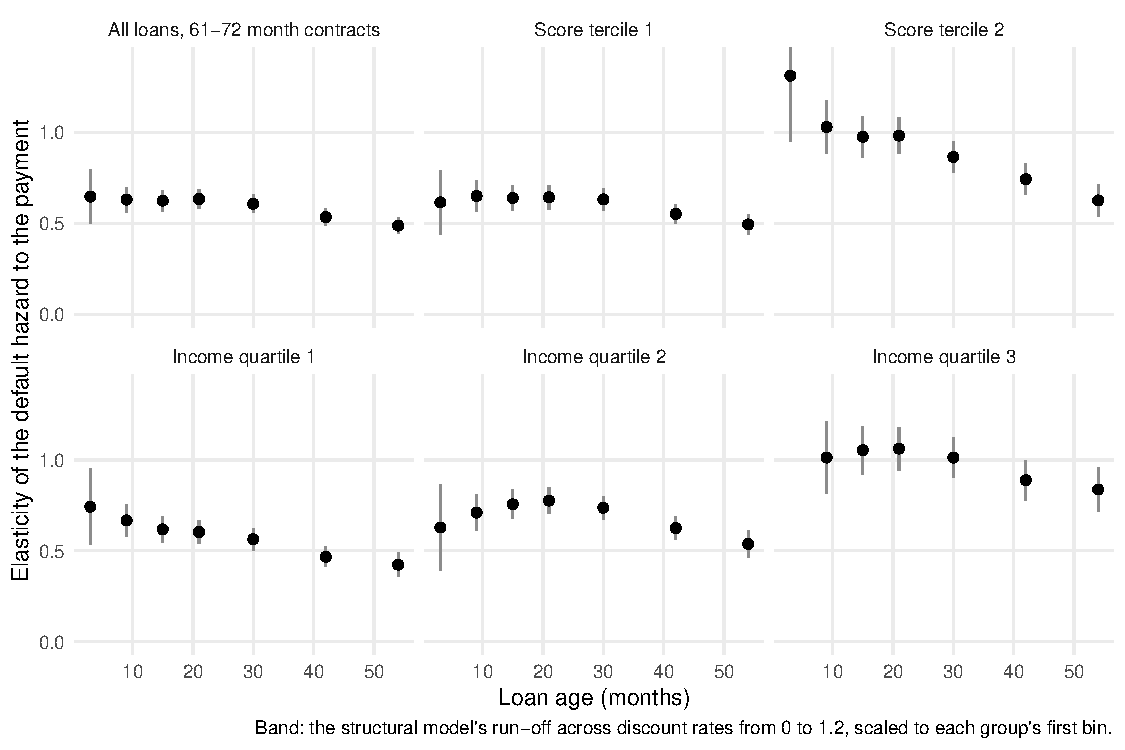
\includegraphics[width=\textwidth]{figures/fig_runoff_profiles.pdf}
\caption{The payment margin over the life of the loan, 61--72 month contracts. Points: elasticity of the charge-off hazard within each loan-age bin to the payment, among loans surviving to the bin, with 95 percent bands. Band: the stopping model's decline across discount rates from zero to $1.2$ with independent income, scaled to each group's first bin.}
\label{fig:runoff_profiles}
% replication: Code/type/T1i_runoff_panel.R, Code/local/mc_runoff_model_grid.R, Code/exhibits/make_runoff_figures.R
\end{figure}

Figure \ref{fig:runoff_shape} reports the ratio of the payment elasticity in the 48- to 60-month bin to the elasticity in the first six months, from each group's own profile on 61- to 72-month contracts, with the 73-month-and-longer contracts alongside, against the range the model of Table \ref{tab:mc_runoff_grid} produces across discount rates; Table \ref{tab:runoff_shape} reports the ratio by group at fixed contract lengths with the set of rates at which the model's decline, scaled to the group's first bin, lies within the $\chi^2(1)$ cut of the group's profile. The ratio lies between $0.57$ and $0.93$ in every group with seven loan-age bins, the 95 percent bands overlap the model's range throughout, and the inversion returns the whole grid of rates in every group except the 49- to 60-month contracts, the middle score tercile, the bottom income quartile and the 2005--09 cohort, where the model's shape fits less well and the set is bounded above; in those groups the profile falls faster than the model at any rate, which is the direction in which the persistent income process of Appendix \ref{appendix:persistent} moves the model, there to a ratio of $0.2$, below every group's. Table \ref{tab:persistent_extract} sets the two calibrations beside the data: the independent-income version reproduces the decline and not the timing of default, the persistent version reproduces the timing and not the decline, and neither reaches the payment elasticity. Neither comparison assigns a rate to a group.

\begin{figure}[H]
\centering
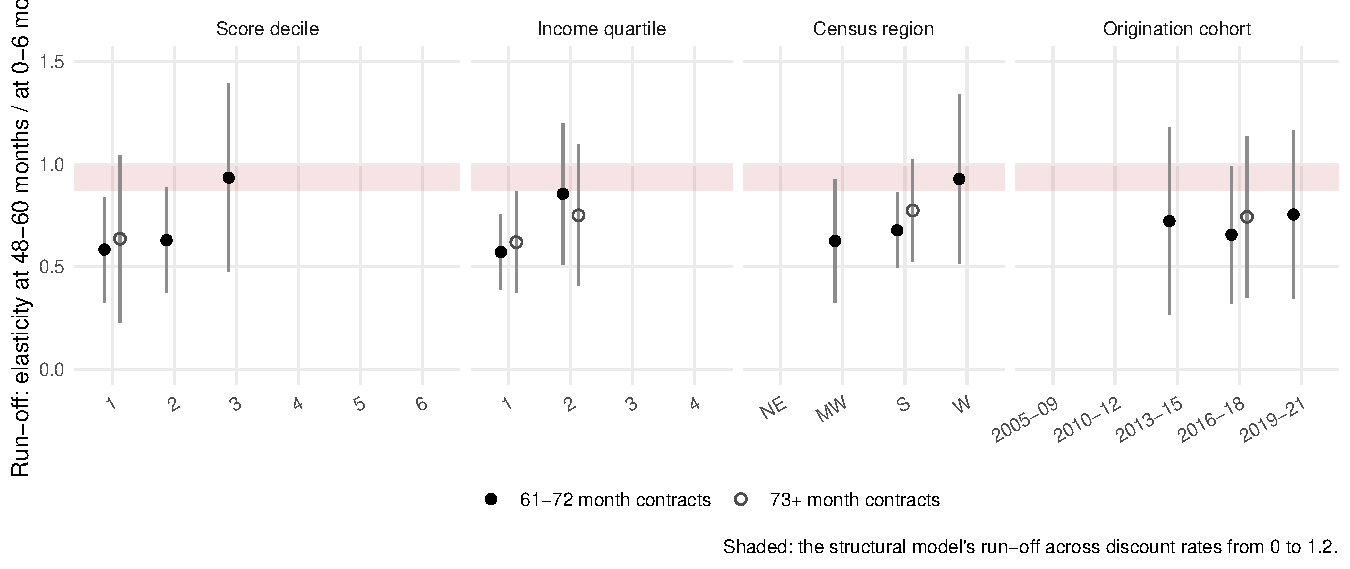
\includegraphics[width=\textwidth]{figures/fig_runoff_shape.pdf}
\caption{The ratio of the payment elasticity at 48--60 months to the elasticity at 0--6 months, by score decile, income quartile, census region and origination cohort, on 61--72 month contracts (filled) and on contracts of 73 months and longer (hollow), with 95 percent bands. Shaded: the model's ratio across discount rates from zero to $1.2$ with independent income.}
\label{fig:runoff_shape}
% replication: Code/exhibits/make_runoff_figures.R
\end{figure}

\begin{table}[H]
\centering
\caption{The decline of the payment elasticity by group at fixed contract length, and the set of discount rates at which the model reproduces it}
\label{tab:runoff_shape}
\small
\begin{tabular}{llrrr}
\toprule
Dimension & Group & Run-off (48--60 / 0--6) & Model set for $\rho$ & $\chi^2$/df \\
\midrule
All loans, by contract length & 49-60 months & 0.65 & [0.71, $\ge 1.2$] & 29.8/5 \\
 & 61-72 months & 0.75 & [0.72, $\ge 1.2$] & 9.7/5 \\
 & 73+ months & 0.77 & [0.00, $\ge 1.2$] & 1.2/5 \\
\addlinespace
Score decile & 1 & 0.58 (0.13) & [0.21, $\ge 1.2$] & 9.3/5 \\
 & 2 & 0.63 (0.13) & [0.00, $\ge 1.2$] & 3.0/5 \\
 & 3 & 0.93 (0.23) & [0.58, $\ge 1.2$] & 7.9/5 \\
 & 4 & -- & [0.28, $\ge 1.2$] & 12.4/4 \\
 & 5 & -- & [0.00, $\ge 1.2$] & 6.0/4 \\
 & 6 & -- & [0.00, $\ge 1.2$] & 9.8/4 \\
\addlinespace
Income quartile & 1 & 0.57 (0.09) & [0.50, $\ge 1.2$] & 18.3/5 \\
 & 2 & 0.86 (0.18) & [0.69, $\ge 1.2$] & 17.4/5 \\
 & 3 & -- & [0.07, $\ge 1.2$] & 4.2/4 \\
 & 4 & -- & [0.00, $\ge 1.2$] & 7.9/4 \\
\addlinespace
Census region & NE & -- & [0.00, $\ge 1.2$] & 1.7/4 \\
 & MW & 0.63 (0.15) & [0.34, $\ge 1.2$] & 14.7/5 \\
 & S & 0.68 (0.09) & [0.35, $\ge 1.2$] & 7.3/5 \\
 & W & 0.93 (0.21) & [0.56, $\ge 1.2$] & 5.1/5 \\
\addlinespace
Origination cohort & 2005-09 & -- & [0.39, $\ge 1.2$] & 30.4/4 \\
 & 2010-12 & -- & [0.00, $\ge 1.2$] & 0.6/4 \\
 & 2013-15 & 0.72 (0.23) & [0.00, $\ge 1.2$] & 3.4/5 \\
 & 2016-18 & 0.66 (0.17) & [0.00, $\ge 1.2$] & 3.0/5 \\
 & 2019-21 & 0.76 (0.21) & [0.00, $\ge 1.2$] & 1.6/5 \\
\bottomrule
\end{tabular}

\vspace{0.5em}
\begin{minipage}{0.92\textwidth}
\noindent \small \textit{Notes:} Run-off: the payment elasticity in the 48--60 month bin over the 0--6 month bin (delta-method standard error). Model set: the discount rates on the grid from zero to $1.2$ at which the model's ratio, scaled to the group's first bin, lies within the $\chi^2(1)$ cut of the group's profile.
\end{minipage}
% replication: Code/local/runoff_model_inversion.R, Code/exhibits/make_runoff_figures.R
\end{table}

\begin{table}[H]
\centering
\caption{The two calibrations of the stopping model beside the data: what each reproduces}
\label{tab:persistent_extract}
\small
\begin{tabular}{lrrrr}
\toprule
 & \multicolumn{2}{c}{i.i.d.\ income} & Persistent income & Data \\
\cmidrule(lr){2-3}
 & model & i.i.d.\ limit & (calibrated) & \\
\midrule
Payment elasticity, default within 12 months & 4.53 & 4.38 & 4.59 & 0.45 \\
Lifetime default (targeted) & 0.048 & 0.048 & 0.048 & 0.048 \\
Share of lifetime default within 12 months (targeted in the persistent version) & 0.93 & 0.96 & 0.13 & 0.13 \\
Run-off ratio, 48--60 over 0--6 months &  &  & 0.22 & 0.75 \\
Monthly hazard, month 12 over month 1 &  & 0.01 & 10.00 & 6.05 \\
Monthly hazard, month 60 over month 12 &  & 0.30 & 1.39 & 1.30 \\
\bottomrule
\end{tabular}

\vspace{0.5em}
\begin{minipage}{0.92\textwidth}
\noindent \small \textit{Notes:} An extract of Table \ref{tab:persistent_calibration} (Appendix \ref{appendix:persistent}). The i.i.d.\ model is the simulated model of this appendix with the penalty calibrated to lifetime default; the i.i.d.\ limit is the persistent solver at zero persistence; the persistent version is calibrated to lifetime default and to the first-year share. Data: the auto-loan panel. The i.i.d.\ model's payment elasticity is the hazard-bin elasticity in the first bin; the other columns report the elasticity of default within twelve months.
\end{minipage}
% replication: Code/exhibits/make_persistent_tables.R
\end{table}

% appendix_persistent.tex: the stopping model with a persistent income state: calibration, the run-off, the window ratios (2026-09-10).
% Placed inside Appendix \ref{appendix:mcliquidity}, after the subsection "Calibration to the level of the payment margin".
\subsection{Persistent income: what it changes and what it does not}\label{appendix:persistent}

The model of Tables \ref{tab:mc_runoff_grid} and \ref{tab:mc_runoff_grid2} draws income independently each month. Calibrated to the panel's lifetime charge-off rate, it places $0.93$ of lifetime default in the first year of the loan, against the panel's $0.13$, and its payment elasticity within twelve months is $4.4$ to $5.4$, against the panel's $0.45$. This subsection replaces the independent draw with a persistent income state, calibrates the model to the lifetime rate and to the first-year share, and reports the timing of default, the payment and term elasticities, the run-off of the payment elasticity by loan age, and the term-to-payment ratios $R_{12}$, $R_{24}$ and $R_{36}$ of Table \ref{tab:within_by_group}. Replication: \path{Code/local/mc_persistent_model.R}, \path{Code/exhibits/make_persistent_tables.R}, \path{results/mc_persistent_*.csv}.

\paragraph{The model with an income state.} Log income is the sum of a persistent state and a transitory shock,
\begin{equation}\label{eq:persistent_income}
\log y_t = z_t + \varepsilon_t, \qquad z_{t+1} = \phi\, z_t + \nu_{t+1}, \qquad \nu_{t+1} \sim N(0, s_z^2), \qquad \varepsilon_t \sim N(0, s_\varepsilon^2),
\end{equation}
with $\phi$ the monthly persistence, $s_z$ the standard deviation of the innovation and $s_\varepsilon$ that of the transitory shock, both i.i.d. Median income is one, the payment is a constant $r$ in units of median income, utility is logarithmic, and the borrower starts at her persistent level, $z_1 = 0$, since the lender sets the payment against income at origination; the cross-section of $r$ represents the population's heterogeneity in the payment-to-income ratio. The value of standing $K_t$ of equation \eqref{eq:Krec}, with the balance-scaled penalty of Appendix \ref{appendix:balancepenalty} and a logistic taste shock of scale $s$ on the default margin, becomes a function of the state,
\begin{equation}\label{eq:persistent_K}
K_t(z) = \sigma + \pi_t + \delta s_x \sum_{z'} P(z, z')\, \mathbb{E}_{\varepsilon}\Big[\, s \log\big(1 + e^{(K_{t+1}(z') - g(y'))/s}\big) \,\Big], \qquad K_T(z) = \sigma A_T + \pi_T,
\end{equation}
where $g(y) = u(y) - u(y - r)$ is the utility cost of paying, infinite when $y \le r$, so that default is forced there; $P(z, z')$ is the transition of the discretized state; $\delta = e^{-\rho/12}$ at the annual rate $\rho$; $s_x = e^{-h/12}$ is survival to the next payment at the exit hazard $h = 0.22$ per year; $\pi_t = \kappa_B (b_t - \delta s_x b_{t+1})$ is the one-time balance penalty with $b_t$ the annuity balance at a six percent note rate; and $A_T = \sum_{k=0}^{H-T}\delta^k$ discounts the penalty flow $\sigma$ over the fixed horizon $H = 120$ months. The term inside the expectation is the expected surplus from standing under the taste shock, in place of the positive part in \eqref{eq:Krec}. The borrower defaults at $t$ with probability $p_t(z) = \mathbb{E}_\varepsilon[\Lambda((g(y) - K_t(z))/s)]$, $\Lambda$ the logistic distribution function, and the population over the state evolves as $\mu_{t+1} = s_x P'(\mu_t (1 - p_t))$, so that every moment is a deterministic function of the parameters. The conventions are those of the i.i.d.\ model: $s = 0.5\sigma$, $\log r \sim N(\log 0.1, 0.47^2)$, and $T \in \{48, 60, 72\}$ with weights one quarter, one half, one quarter. The payment elasticity of default within $K$ months is the population mean of $\partial d_K/\partial \log r$ over the mean of $d_K$, the term elasticity is the central difference in $\log T$ at a fixed payment, $R_K$ is their ratio, and the run-off is the elasticity of the bin hazard among survivors on 72-month contracts, 48--60 months over 0--6. At $\phi = s_z = 0$ and $s_\varepsilon = 0.5$ the solver reproduces the hazard paths of \path{Code/local/mc_model_recovery.R} (\path{results/mc_persistent_check.csv}); its moments are the second column of Table \ref{tab:persistent_calibration}.

\paragraph{Calibration.} The targets are the panel's lifetime charge-off rate, $0.048$, and the share of lifetime charge-offs within twelve months, $0.126$ (45,946 of 365,312; \path{results/panel_windows_auto.csv}), at $\rho = 0.09$, $\kappa_B = 0$ and $s_\varepsilon = 0.2$; $(s_z, \sigma)$ are fitted at each $\phi$ on a grid from $0.95$ to $0.998$ (\path{results/mc_persistent_calibration.csv}, rows \texttt{share\_fit\_phi*}). At $\phi \le 0.98$ the share is not reached: raising $s_z$ lowers the first-year share but raises the mass of borrowers whose income falls below the payment at some date, default that no $\sigma$ removes, and that mass exceeds the lifetime target first, so the fit stops at shares of $0.23$, $0.18$ and $0.14$ at $\phi = 0.95$, $0.97$ and $0.98$. At $\phi \ge 0.99$ both targets are met, and $\phi = 0.998$ is the fit whose monthly hazard by loan age is closest to the panel's (\path{results/mc_persistent_hazard.csv}). The calibrated process has $\phi = 0.998$ per month, $0.976$ per year; $s_z = 0.147$, an annual innovation standard deviation of $0.50$ and a standard deviation of $z$ after 72 months of $1.16$; and $\sigma = 0.476$. Table \ref{tab:persistent_calibration} sets it beside the i.i.d.\ model, the i.i.d.\ limit of the same solver, and the data. It matches the first-year share ($0.127$), gives a 24-month share of $0.41$ against the panel's $0.36$, and has a monthly hazard that rises tenfold from the first month to the twelfth and is flat after, at $1.39$ times the twelfth-month level in the sixtieth month, where the panel's rises sixfold and is then flat at $1.30$ times; the i.i.d.\ versions place $0.93$ to $0.96$ of lifetime default in the first year with a hazard that falls from the first month.

\begin{table}[H]
\centering
\caption{The stopping model with i.i.d.\ and with persistent income: parameters, targeted and untargeted moments, and the data}
\label{tab:persistent_calibration}
% replication: Code/local/mc_persistent_model.R, Code/exhibits/make_persistent_tables.R; results/mc_persistent_calibration.csv, results/mc_persistent_iid_limit.csv, results/mc_within_grid_v3.csv
\small
\resizebox{0.95\textwidth}{!}{\begin{tabular}{lrrrr}
\toprule
 & \multicolumn{2}{c}{i.i.d.\ income} & Persistent income & Data \\
\cmidrule(lr){2-3}
 & i.i.d.\ model & i.i.d.\ limit of the & (calibrated) & \\
 & (simulated) & persistent solver & & \\
\midrule
\multicolumn{5}{l}{\emph{Parameters}} \\
Annual rate $\rho$ at calibration & 0.10 & 0.09 & 0.09 &  \\
Persistence $\phi$ (monthly) & 0 & 0 & 0.998 &  \\
Innovation s.d.\ $s_z$ & 0 & 0 & 0.147 &  \\
Transitory s.d.\ $s_\varepsilon$ & 0.5 & 0.50 & 0.20 &  \\
Penalty flow $\sigma$ & 0.251 & 0.236 & 0.476 &  \\
Taste-shock scale $s/\sigma$ & 0.5 & 0.50 & 0.50 &  \\
Balance penalty $\kappa_B$ & 0 & 0 & 0 &  \\
\addlinespace
\multicolumn{5}{l}{\emph{Targeted moments}} \\
Lifetime default & 0.048 & 0.048 & 0.048 & 0.048 \\
Share of lifetime default within 12 months$^{a}$ & 0.93 & 0.96 & 0.13 & 0.13 \\
\addlinespace
\multicolumn{5}{l}{\emph{Untargeted moments}} \\
Share within 24 months & 0.96 & 0.98 & 0.41 & 0.36 \\
Payment elasticity, default within 12 months & 4.53$^{b}$ & 4.38 & 4.59 & 0.45 \\
Payment elasticity, lifetime default &  & 4.33 & 2.22 & 0.35 \\
Term elasticity, default within 12 months$^{c}$ &  & +2.48 & +1.30 & -0.31 \\
$R_{12}$, term over payment elasticity$^{c}$ & +0.464 & +0.565 & +0.284 & -0.70 (0.02) \\
$R_{24}$ & +0.473 & +0.562 & +0.388 & +0.55 (0.01) \\
$R_{36}$ & +0.459 & +0.553 & +0.484 &  \\
Run-off ratio (48--60 over 0--6 months)$^{d}$ &  &  & 0.22 & 0.75 \\
Monthly hazard, month 12 over month 1 &  & 0.01 & 10.00 & 6.05 \\
Monthly hazard, month 60 over month 12 &  & 0.30 & 1.39 & 1.30 \\
\bottomrule
\end{tabular}
}
\vspace{0.5em}
\begin{minipage}{0.95\textwidth}
\noindent \small \textit{Notes:} The i.i.d.\ model: the simulated model of Tables \ref{tab:mc_runoff_grid} and \ref{tab:mc_runoff_grid2} with $\sigma$ calibrated to lifetime default at $\rho = 0.10$ (\path{results/mc_within_grid_v3.csv}, \path{mc_runoff_model_grid_h0.22.csv}). i.i.d.\ limit: the solver of this subsection at $\phi = s_z = 0$, $s_\varepsilon = 0.5$ (\path{results/mc_persistent_iid_limit.csv}). Persistent: the calibrated process (\path{results/mc_persistent_calibration.csv}, row \texttt{calibrated}). Data: the auto-loan panel (\path{results/panel_windows_auto.csv}, \path{identification_within_person_by_group.csv}, \path{runoff_model_rho_co_h0.22.csv}, \path{hazard_by_month.csv}). $^{a}$ Targeted in the persistent version only. $^{b}$ The hazard-bin elasticity in the 0- to 6-month bin of Table \ref{tab:mc_runoff_grid}, the i.i.d.\ model's estimator; the other columns report the elasticity of default within twelve months. $^{c}$ Data: within-borrower estimates of Table \ref{tab:within_by_group}; the pooled fixed-effects term elasticity within twelve months is $+0.01$ ($0.05$); standard errors of the ratios by the delta method. $^{d}$ Data: 61- to 72-month contracts, Table \ref{tab:runoff_shape}. The i.i.d.\ limit's run-off is not reported: with $0.96$ of default in the first year, the bin hazards among survivors after the first year are ratios of vanishing masses. The last two rows are ratios of the monthly hazard by loan age.
\end{minipage}
\end{table}

\paragraph{The payment elasticity.} The persistent version's payment elasticity within twelve months is $4.59$, ten times the panel's $0.45$; over the life of the loan it is $2.22$ against $0.35$; and its term elasticity within twelve months is $+1.30$ against the within-borrower $-0.31$. The elasticity does not move with the income process. Over the 34 feasible points of the $(\phi, s_z)$ scan, $\phi$ from $0.95$ to $0.998$ and $s_z$ from $0.03$ to $0.25$ with $\sigma$ calibrated to the lifetime rate at each point, the elasticity within twelve months lies in $[4.12, 4.60]$ while the first-year share runs from $0.998$ to $0.110$ and the run-off ratio from $71$ to $0.21$; at $s_\varepsilon = 0.1$ and $0.3$ with $s_z$ re-fitted to the share it is $4.50$ and $4.73$ (rows \texttt{scan}, \texttt{s\_eps\_*}). The reason is in \eqref{eq:persistent_K}: the value of standing moves with the persistent state by a multiple of $g$ of order $1/(1 - \delta s_x \phi)$, between ten and forty at these persistences, against a taste shock of scale $0.5\sigma$, so default is a threshold crossing in income at every $\phi$, and the elasticity of a threshold-crossing probability is the ratio of the density to the mass at the threshold, $2.1$ at a mass of five percent for a normal variable in units of its standard deviation: an elasticity of $4$ to $5$ corresponds to a dispersion of log income at the threshold of $0.4$ to $0.5$ log points, and $0.45$ to a dispersion near $4.6$, which no process on the scan approaches. The taste-shock scale is the one lever that changes this (rows \texttt{taste\_*}): at $s/\sigma = 1$, $2$ and $4$ the elasticity is $4.59$, $4.54$ and $3.52$ with the share matched, and at $s/\sigma = 6$ it is $0.71$, with $\sigma = 3.2$, a first-year share of $0.30$ that no $s_z$ brings to the target, $R_{12} = 2.84$ and a run-off of $1.66$. The panel's elasticity is not reached with the share matched in either version.

\paragraph{The run-off.} Table \ref{tab:persistent_runoff} reports the run-off ratio on the $(\rho, \kappa_B)$ grid with $\sigma$ re-calibrated to the lifetime rate at each point, and the profile by loan-age bin at $\rho = 0.10$. In the persistent version the ratio is between $0.20$ and $0.22$ at every rate from $0.02$ to $0.8$ and every $\kappa_B$ from $0$ to $0.2$: it moves by $0.015$ across the rate grid and by $0.002$ across the penalty. In the i.i.d.\ model it is between $0.87$ and $0.99$ at every rate from $0$ to $1.2$ (Table \ref{tab:mc_runoff_grid}); the panel's is $0.75$. The insensitivity to the rate is the same in the two versions; the level and the shape are not. The persistent version's elasticity falls from the first bin, to $0.71$ of its initial level in the 6- to 12-month bin, $0.43$ in the 18- to 24-month bin and $0.21$ in the last, where the panel's stays within $0.06$ of its initial level for three years and then falls to $0.75$, and the i.i.d.\ model's declines to $0.77$.

\begin{table}[!ht]
\centering
\caption{The run-off of the payment elasticity: by discount rate and balance penalty, and by loan-age bin}
\label{tab:persistent_runoff}
% replication: Code/local/mc_persistent_model.R, Code/exhibits/make_persistent_tables.R; results/mc_persistent_grid.csv, results/mc_runoff_model_grid_h0.22.csv, results/runoff_model_rho_co_h0.22.csv
\small
\textit{Panel A: the ratio, 48--60 over 0--6 months, by discount rate}\\[0.4em]
\resizebox{0.95\textwidth}{!}{\begin{tabular}{lrrrrrrrrrrr}
\toprule
Annual rate $\rho$ & 0.00 & 0.02 & 0.05 & 0.10 & 0.20 & 0.30 & 0.35 & 0.50 & 0.55 & 0.80 & 1.20 \\
\midrule
i.i.d.\ income & 0.87 &  & 0.93 & 0.96 & 0.94 &  & 0.93 &  & 0.92 & 0.96 & 0.99 \\
Persistent income, $\kappa_B = 0$ &  & 0.22 & 0.22 & 0.22 & 0.21 & 0.21 &  & 0.21 &  & 0.20 &  \\
Persistent income, $\kappa_B = 0.05$ &  & 0.22 & 0.22 & 0.21 & 0.21 & 0.21 &  & 0.21 &  & 0.20 &  \\
Persistent income, $\kappa_B = 0.2$ &  & 0.22 & 0.22 & 0.22 & 0.21 & 0.21 &  & 0.21 &  & 0.20 &  \\
\midrule
Data, 61--72-month contracts & \multicolumn{11}{l}{0.75} \\
\bottomrule
\end{tabular}
}\\[0.8em]
\textit{Panel B: the profile by loan-age bin at $\rho = 0.10$}\\[0.4em]
\resizebox{0.95\textwidth}{!}{\begin{tabular}{lrrrrrrr}
\toprule
Loan-age bin (months) & 0--6 & 6--12 & 12--18 & 18--24 & 24--36 & 36--48 & 48--60 \\
\midrule
\multicolumn{8}{l}{\emph{Payment elasticity of the bin hazard among survivors}} \\
Data, 61--72-month contracts & 0.65 & 0.63 & 0.63 & 0.64 & 0.61 & 0.54 & 0.49 \\
i.i.d.\ income, $\rho = 0.10$ & 4.53 & 4.43 & 4.11 & 4.09 & 4.45 & 4.34 \\
Persistent income, $\rho = 0.10$, $\kappa_B = 0$ & 5.96 & 4.26 & 3.18 & 2.54 & 1.96 & 1.53 & 1.28 \\
\addlinespace
\multicolumn{8}{l}{\emph{Relative to the 0--6 month bin}} \\
Data & 1.00 & 0.97 & 0.97 & 0.98 & 0.94 & 0.83 & 0.75 \\
i.i.d.\ income & 1.00 & 0.98 & 0.91 & 0.90 & 0.98 & 0.96 \\
Persistent income & 1.00 & 0.71 & 0.53 & 0.43 & 0.33 & 0.26 & 0.21 \\
\bottomrule
\end{tabular}
}
\vspace{0.5em}
\begin{minipage}{0.95\textwidth}
\noindent \small \textit{Notes:} Panel A: the i.i.d.\ model from Table \ref{tab:mc_runoff_grid} (\path{results/mc_runoff_model_grid_h0.22.csv}); the persistent version at the calibrated income process with $\sigma$ re-fitted to lifetime default at each $(\rho, \kappa_B)$ (\path{results/mc_persistent_grid.csv}); the data from Table \ref{tab:runoff_shape}. Panel B: the elasticity of the charge-off hazard to the payment among loans surviving to each bin; the data's row is the 61- to 72-month contracts of Figure \ref{fig:runoff_profiles} (\path{results/runoff_model_rho_co_h0.22.csv}).
\end{minipage}
\end{table}

\paragraph{The window ratios.} Table \ref{tab:persistent_windows} reports $R_{12}$, $R_{24}$ and $R_{36}$ on the $(\rho, \kappa_B)$ surface for both versions, with the panel's within-borrower pair. In the i.i.d.\ model the three ratios are the same at each point for $\kappa_B \le 0.2$, $R_{36} - R_{12}$ between $-0.05$ and $+0.19$, because with $0.93$ of default in the first year the windows differ only in months that contain almost no default; at $\kappa_B = 0.5$, where the penalty spreads default over the first two years and the first-year share is $0.50$ at $\rho = 0.10$, the rise reaches $0.27$ at that rate. In the persistent version the ratio rises with the window at every point of the surface: $R_{36} - R_{12}$ is between $0.10$ and $0.26$, and $R_{24} - R_{12}$ between $0.03$ and $0.13$, largest at low rates and high penalties. All three ratios fall with the rate, $R_{12}$ from $0.37$ at $\rho = 0.02$ to $0.015$ at $\rho = 0.8$ with $\kappa_B = 0$, and the balance penalty lowers each; $R_{12}$ is negative at $(\kappa_B, \rho) = (0.05, 0.8)$, $(0.2, 0.5)$ and $(0.2, 0.8)$, and its minimum on the surface is $-0.099$, where $R_{24} = -0.057$. The panel's pair is $R_{12} = -0.70$ ($0.02$) and $R_{24} = +0.55$ ($0.01$), a rise of $1.25$ from the first window to the second. The smallest $R_{12}$ on the surface is $0.60$ above the panel's, 28 standard errors; the largest $R_{24}$, $0.477$ at $(\kappa_B, \rho) = (0, 0.02)$, is $0.08$ below the panel's, 7 standard errors, with $R_{12} = +0.37$ at that point; and the sign change between the two windows occurs on the surface only at $(0.05, 0.8)$ and $(0.2, 0.5)$, with magnitudes below $0.06$. The persistent version produces the feature the i.i.d.\ version does not, a ratio that rises with the window, at one tenth of the panel's amplitude.

\begin{table}[!ht]
\centering
\caption{The term-to-payment ratios $R_{12}$, $R_{24}$ and $R_{36}$ by discount rate and balance penalty, i.i.d.\ and persistent income, with the data's within-borrower pair}
\label{tab:persistent_windows}
% replication: Code/local/mc_persistent_model.R, Code/exhibits/make_persistent_tables.R; results/mc_persistent_grid.csv, results/mc_within_grid_v3.csv, results/identification_within_person_by_group.csv
\scriptsize
\resizebox{0.9\textwidth}{!}{\begin{tabular}{rrrrrrrrrr}
\toprule
 & & \multicolumn{4}{c}{i.i.d.\ income} & \multicolumn{4}{c}{Persistent income} \\
\cmidrule(lr){3-6} \cmidrule(lr){7-10}
$\kappa_B$ & $\rho$ & $R_{12}$ & $R_{24}$ & $R_{36}$ & $R_{36} - R_{12}$ & $R_{12}$ & $R_{24}$ & $R_{36}$ & $R_{36} - R_{12}$ \\
\midrule
0 & 0.02 & +0.544 & +0.529 & +0.504 & -0.040 & +0.372 & +0.477 & +0.562 & +0.190 \\
 & 0.10 & +0.464 & +0.473 & +0.459 & -0.004 & +0.273 & +0.376 & +0.474 & +0.200 \\
 & 0.30 & +0.259 & +0.291 & +0.299 & +0.040 & +0.119 & +0.202 & +0.309 & +0.190 \\
 & 0.80 & +0.050 & +0.094 & +0.127 & +0.077 & +0.015 & +0.043 & +0.117 & +0.102 \\
\addlinespace
0.05 & 0.02 & +0.532 & +0.513 & +0.485 & -0.047 & +0.352 & +0.465 & +0.556 & +0.204 \\
 & 0.10 & +0.431 & +0.436 & +0.428 & -0.003 & +0.251 & +0.363 & +0.466 & +0.215 \\
 & 0.30 & +0.196 & +0.241 & +0.260 & +0.063 & +0.092 & +0.184 & +0.297 & +0.205 \\
 & 0.80 & -0.065 & -0.009 & +0.046 & +0.111 & -0.020 & +0.016 & +0.097 & +0.116 \\
\addlinespace
0.2 & 0.02 & +0.464 & +0.464 & +0.453 & -0.010 & +0.294 & +0.428 & +0.538 & +0.244 \\
 & 0.10 & +0.295 & +0.359 & +0.370 & +0.074 & +0.188 & +0.321 & +0.444 & +0.256 \\
 & 0.30 & -0.054 & +0.057 & +0.127 & +0.182 & +0.021 & +0.130 & +0.263 & +0.242 \\
 & 0.80 & -0.459 & -0.385 & -0.267 & +0.192 & -0.099 & -0.057 & +0.036 & +0.135 \\
\addlinespace
0.5 & 0.02 & +0.136 & +0.269 & +0.331 & +0.195 &  &  &  &  \\
 & 0.10 & -0.135 & +0.022 & +0.135 & +0.270 &  &  &  &  \\
 & 0.30 & -0.468 & -0.383 & -0.241 & +0.227 &  &  &  &  \\
 & 0.80 & -0.397 & -0.612 & -0.651 & -0.254 &  &  &  &  \\
\midrule
\multicolumn{2}{l}{Data, within borrower} & \multicolumn{8}{l}{$R_{12} = -0.70$ (0.02), $R_{24} = +0.55$ (0.01), $R_{24} - R_{12} = 1.25$} \\
\bottomrule
\end{tabular}
}
\vspace{0.5em}
\begin{minipage}{0.95\textwidth}
\noindent \small \textit{Notes:} $R_K$ is the elasticity of default within $K$ months to the contract length over its elasticity to the payment. i.i.d.: the model with $\sigma$ calibrated to lifetime default at $\rho = 0.10$ for each $\kappa_B$, 150,000 simulated loans, the paper's joint regression with cell effects (\path{results/mc_within_grid_v3.csv}). Persistent: the calibrated income process with $\sigma$ re-fitted at each point, population derivatives (\path{results/mc_persistent_grid.csv}, which also holds $\rho = 0.05$, $0.2$ and $0.5$). Data: the within-borrower estimates of Table \ref{tab:within_by_group}, all loans, standard errors by the delta method.
\end{minipage}
\end{table}

\paragraph{What the persistent version establishes.} First, a persistent income state reproduces the timing of default: the first-year share, the 24-month share within $0.05$, and a hazard that rises over the first year and is flat after. Second, it leaves the payment elasticity at $4.1$ to $4.7$ at every persistence, dispersion and taste-shock scale for which the first-year share is matched, ten times the panel's, because default remains a threshold crossing in income; the i.i.d.\ model has the same elasticity for the same reason. Third, the run-off ratio does not move with the rate in either version, and its level and shape in the persistent version, $0.20$ to $0.22$ with a decline from the first bin, are not the panel's $0.75$ with a flat profile for three years, which the i.i.d.\ model reproduces at a first-year share of $0.93$. Fourth, the persistent version separates the windows, by $0.03$ to $0.13$ between $R_{12}$ and $R_{24}$, with the separation moving with $\rho$ and $\kappa_B$; the panel's separation is $1.25$, with a sign change the surface does not contain at any magnitude above $0.06$. The statements elsewhere in this appendix and in the main text that the run-off, the term margin and the equity margin are insensitive to the rate are therefore established in calibrations whose payment elasticity is ten times the panel's, in both versions of the income process, and they are conditional on that calibration. The model is a device for the mechanisms it contains, the option to default later and the balance-scaled penalty, and not a quantitative match to the bureau's margins. The panel's within-borrower window pattern, $-0.70$ at twelve months and $+0.55$ at 24, measured to a few hundredths, is a fact outside the model class at these calibrations; the two moments the class does not reach, the level of the payment elasticity and the amplitude of the window pattern, are the two that depend on the shape of the default margin rather than on the timing of income, and a version in which the default margin is not a threshold in income is the extension they call for. A second reason the calibration cannot be expected to reach the panel's margins is what it draws from: both income processes are calibrated as earnings processes, whereas the model's income is net of non-discretionary expenses, and \citet{fulford_expense_2024} show that expense shocks are at least as frequent and as large as earnings shocks, with shocks above eighty percent of income several times more common than comparable earnings drops. A process measured on earnings alone understates the dispersion and the tail of the net income the default decision responds to, and no measured earnings process can be plugged in to make the model fit. That is a further reason the paper estimates the rate from sufficient statistics that use neither income nor consumption data: the default responses embed the net shock distribution the household actually faces.



\subsection{Heterogeneity in the rate against heterogeneity in default}\label{appendix:rhovariance}

Section \ref{sec:exposure_not_impatience} interprets the differences in default across groups as exposure. This subsection sizes the alternative on the model: how much the discount rate would have to differ across groups, with everything else common, to generate a given share of the observed differences, and how much each of the other primitives would have to differ to generate the same share. The observed differences are those of Table \ref{tab:exposure}'s groups: charge-off within twelve months is $1.60$ percent in the bottom score tercile and $0.03$ percent in the top, a ratio of $53$ (a log gap of $3.97$), and over the life of the loan $12.3$ against $0.24$ percent, a ratio of $51$; across score deciles the standard deviation of log default is $1.29$ within twelve months (seven deciles with a measurable rate) and $1.79$ over the life (ten deciles); across income quartiles the bottom-to-top ratios are $31$ and $21$. The model is the one of Table \ref{tab:mc_runoff_grid} with a common penalty level in every cell, and the penalty scale is calibrated so that lifetime default among originated loans, with exits removed from the risk set, equals the panel's $4.8$ percent at $\rho = 0.09$, the calibration point of the grid; at that point default within twelve months is $4.59$ percent against the panel's $0.62$: the model places almost all of its lifetime default in the first year, where the panel places one eighth of it. Expected default rates are computed exactly from the solved hazard paths on the 300,000-loan population.

Table \ref{tab:rho_variance}, Panel A, reports default on a grid of the rate. Default rises with the rate: within twelve months from $3.31$ percent at $\rho = 0$ to $4.59$ at $0.09$, $12.0$ at $1.2$ and $20.3$ at $3$, and over the life from $3.5$ to $4.8$, $16.8$ and $37.0$ percent. The reason is the timing of the penalty. In the model the fixed cost of default is a flow over the penalty horizon, and a borrower who discounts the future more weighs that flow less and the value of good standing falls with it; the far payments, which she also weighs less, pull in the other direction and are the smaller term. The semi-elasticity of default to the annual rate at the calibration is $3.19$ within twelve months and $3.17$ over the life, and it falls as the rate rises. The rate accounts for a share of the observed variance as follows. A spread from $\rho = 0$ to $1.10$ between the top and bottom score terciles reproduces one tenth of the tercile variance of log default within twelve months, and a spread from $0$ to $0.69$ one tenth of the lifetime variance; one half is not reached at any rate up to $3$ per year, where the model's gap from $\rho = 0$ is $1.82$ log units within twelve months and $2.36$ over the life against the $2.81$ and $2.78$ that one half requires, and the whole gaps of $3.97$ and $3.93$ are out of reach by factors of $e^{2.2}$ and $e^{1.6}$. Linearised at the calibration, one tenth of the variance across score deciles requires a standard deviation of the rate across deciles of $0.13$ within twelve months and $0.18$ over the life, and one half a standard deviation of $0.29$ to $0.40$; the subgroup pairs of Table \ref{tab:rho_subgroups} find no difference in the rate across the score and leverage splits. In levels the account is different, because the variance in levels is the bottom tercile's: the twelve-month gap of $1.6$ percentage points and the lifetime gap of $12$ points are reproduced in full by a spread of the rate from $0$ to $0.11$ and to $1.07$, and one tenth of the level variance by a spread to $0.04$ and to $0.26$, since a rate of $0.5$ raises the model's twelve-month default from $3.3$ to $9.0$ percent without approaching the top tercile's $0.03$.

Panel B reports the same calculation for the other primitives, each moved uniformly for the whole population with the rest held at the calibration. The semi-elasticity of default to the log payment-to-income ratio is $4.19$ within twelve months and $4.14$ over the life, to the log penalty scale $-3.17$ and $-2.98$, and to the log dispersion of monthly income $1.81$ and $2.10$. The whole bottom-to-top tercile log gap is reproduced by a factor of $2.6$ in the payment-to-income ratio ($0.95$ log units, within twelve months and over the life), by a factor of $3.5$ in the penalty scale ($3.7$ over the life), or by a factor of $9.0$ in income dispersion ($6.5$ over the life); one tenth of the decile variance by a standard deviation of $0.10$ to $0.14$ log units in the payment-to-income ratio, $0.13$ to $0.19$ in the penalty and $0.23$ to $0.27$ in income dispersion. These are the model's elasticities, and its payment elasticity is nine times the panel's $0.45$; at the panel's elasticity the payment-to-income ratio would account for the gap only with a spread of $8.8$ log units. The persistent income process of Appendix \ref{appendix:persistent} does not close that gap, so the required spreads in Panel B are stated at the model's elasticity and not at the panel's.

The first-order formula gives a second measure of the rate's sensitivity, and the two are reconciled by the penalty's timing. In the formula of equation \eqref{eq:Ws} the incentive to default is $m W$ with $W = 1 + \lambda\sum_j D(j)Q(j)$, the penalty is paid once at default, and the elasticity of default to the incentive is the measured payment elasticity, so that $d\log p/d\rho = \varepsilon_m\, d\log W/d\rho = -\varepsilon_m\,\lambda\sum_j (j/12) D(j) Q(j)/W$; at $\rho = 0.09$, $h = 0.22$, $T = 60$ and $\lambda = 0.33$ the second factor is $-1.72$ ($-1.63$ at $\lambda = 0.2$), the far payments' share of the incentive being $0.91$ with a duration of $1.9$ years, so the semi-elasticity is $-0.78$ at the panel's $\varepsilon_m = 0.45$ and $-7.2$ at the model's $4.2$: negative, because in the formula a more impatient borrower cares less about escaping the far payments and nothing else in her decision depends on the rate. The model's own comparative static for the first-month hazard, $d\log p_1/d\rho = 1.96$, is positive because the fixed cost of default is a flow over the penalty horizon, which a more impatient borrower weighs less. Solved with the penalty paid once at the date of default, with the same lifetime default rate, the model's semi-elasticity is $-9.7$ for the first-month hazard, against the formula's $-7.2$ at the model's elasticity, and $-6.6$ within twelve months and $-6.0$ over the life; the sign and the magnitude of the rate's effect on the level of default are therefore properties of how the cost of default is spread over time, which the data of this paper do not measure, and the required spreads in Panel B are of the same order under either timing. Replication: \texttt{Code/local/mc\_rho\_variance.R}, \texttt{results/mc\_rho\_variance.csv}.

\begin{table}[H]
\centering
\caption{The variation in the discount rate, and in the other primitives, that would reproduce the observed variation in default across score groups}
\label{tab:rho_variance}
\scriptsize
\resizebox{\textwidth}{!}{\begin{tabular}{lrrrrrr}
\toprule
\multicolumn{7}{l}{\emph{Panel A. Default in the model on a grid of the discount rate, everything else common}} \\
True annual rate $\rho$ & \multicolumn{2}{c}{default rate (\%)} & \multicolumn{2}{c}{log gap from $\rho = 0$} & \multicolumn{2}{c}{share of the tercile log variance} \\
 & 12 months & lifetime & 12 months & lifetime & 12 months & lifetime \\
\midrule
0.00 & 3.308 & 3.50 & 0.00 & 0.00 & 0.000 & 0.000 \\
0.02 & 3.582 & 3.77 & 0.08 & 0.07 & 0.000 & 0.000 \\
0.05 & 4.005 & 4.20 & 0.19 & 0.18 & 0.002 & 0.002 \\
0.09 & 4.592 & 4.80 & 0.33 & 0.32 & 0.007 & 0.006 \\
0.15 & 5.458 & 5.72 & 0.50 & 0.49 & 0.016 & 0.016 \\
0.20 & 6.140 & 6.47 & 0.62 & 0.61 & 0.024 & 0.024 \\
0.30 & 7.333 & 7.89 & 0.80 & 0.81 & 0.040 & 0.043 \\
0.40 & 8.282 & 9.17 & 0.92 & 0.96 & 0.053 & 0.060 \\
0.55 & 9.318 & 10.82 & 1.04 & 1.13 & 0.068 & 0.082 \\
0.80 & 10.505 & 13.19 & 1.16 & 1.33 & 0.085 & 0.114 \\
1.20 & 12.014 & 16.75 & 1.29 & 1.57 & 0.105 & 0.159 \\
2.00 & 15.263 & 24.83 & 1.53 & 1.96 & 0.148 & 0.248 \\
3.00 & 20.332 & 36.98 & 1.82 & 2.36 & 0.209 & 0.360 \\
\midrule
\multicolumn{7}{l}{\emph{Panel B. The spread in each primitive that reproduces a share of the observed variance of log default across score deciles}} \\
Primitive & \multicolumn{2}{c}{semi-elasticity of default} & \multicolumn{2}{c}{12-month: sd for 10\%, 50\%} & \multicolumn{2}{c}{lifetime: sd for 10\%, 50\%} \\
 & 12 months & lifetime & 10\% & 50\% & 10\% & 50\% \\
\midrule
Discount rate $\rho$ (per unit of the annual rate) & 3.19 & 3.17 & 0.13 & 0.29 & 0.18 & 0.40 \\
Payment-to-income ratio (per log unit) & 4.19 & 4.14 & 0.10 & 0.22 & 0.14 & 0.31 \\
Penalty scale $\sigma$ (per log unit) & -3.17 & -2.98 & 0.13 & 0.29 & 0.19 & 0.42 \\
Income dispersion $s$ (per log unit) & 1.81 & 2.10 & 0.23 & 0.50 & 0.27 & 0.60 \\
$\rho$, penalty paid once at default (per unit of the annual rate) & -6.59 & -5.98 & 0.06 & 0.14 & 0.09 & 0.21 \\
$\rho$, first-order formula, $\varepsilon_m = 0.45$ (data), $\lambda = 0.33$ & -0.78 & -0.78 & 0.53 & 1.18 & 0.73 & 1.63 \\
$\rho$, first-order formula, $\varepsilon_m = 4.19$ (model), $\lambda = 0.33$ & -7.23 & -7.23 & 0.06 & 0.13 & 0.08 & 0.18 \\
\midrule
Observed: sd of log default across score deciles & & & \multicolumn{2}{c}{1.29 (7 deciles)} & \multicolumn{2}{c}{1.79 (10 deciles)} \\
Observed: bottom over top score tercile & & & \multicolumn{2}{c}{53 (log gap 3.97)} & \multicolumn{2}{c}{51 (log gap 3.93)} \\
\bottomrule
\end{tabular}
}
\vspace{0.5em}
\begin{minipage}{0.95\textwidth}
\noindent \small \textit{Notes:} The model of Table \ref{tab:mc_runoff_grid} with a common penalty level, calibrated to lifetime default of $4.8$ percent at $\rho = 0.09$; expected default computed from the solved hazard paths on the 300,000-loan population, with exits at $0.22$ per year removed from the risk set. Panel A: the log gap is $\log p(\rho) - \log p(0)$, and its share of the tercile variance is the square of the gap over the observed bottom-to-top score-tercile log gap ($3.97$ within twelve months, $3.93$ over the life). Panel B: semi-elasticities of log default at the calibration by central differences (the rate in units of the annual rate, the others in log units); the standard deviation of the primitive across score deciles that reproduces the stated share of the observed variance of log default across deciles is $\sqrt{\text{share}}$ times the observed standard deviation over the semi-elasticity. The first-order rows use $d\log p/d\rho = \varepsilon_m\,d\log W/d\rho$ with $W$ from equation \eqref{eq:Ws} at $h = 0.22$ and $T = 60$.
\end{minipage}
% replication: Code/local/mc_rho_variance.R
\end{table}

% appendix_priority.tex: priority of the theoretical results (2026-09-09).
% Companion: memos/priority_ledger_2026-09-09.md (table, verification status, missing bib entries).
% Citations without a key in references.bib are written in plain text; the entries are listed in the memo.
% Input in main.tex after appendix_strategies.

\section{Priority of the Theoretical Results}\label{appendix:priority}

This appendix records, for each theoretical result in the paper, the closest prior statement of the insight and the increment the paper makes. The purpose is to place the results rather than to claim them: several are special cases of known principles, and the appendix says which.

\paragraph{Sensitivities to the payment schedule (Proposition \ref{prop:sensT}).} The device of interpreting a ratio of two behavioral responses as a ratio of marginal utilities is that of \citet{chetty_moral_2008}, who separates the liquidity and moral-hazard components of the response of job search to a benefit by comparing it with the response to a cash grant at the same date, and of \citet{indarte_moral_2023}, who applies the same comparison to bankruptcy filing with a dollar of payment relief and a dollar of seizable equity, both valued at the filing date (her equation (14)). \citet{ganong_liquidity_2020} supply the two-date empirical comparison, payment reduction against principal reduction, and interpret it through liquidity and wealth. In each case the transfers compared are located at one date or are not indexed by their date. Proposition \ref{prop:sensT} locates the transfer at an arbitrary future date in the optimal-stopping default problem and shows that the response factors into the discount function $D(s-1)$, the probability $Q_s$ of still being in good standing, and the average marginal utility of a repayer at $s$ relative to that of the marginal defaulter today; the two-period identity $A/(A+B) = \delta\lambda$ of Section \ref{sec:suffstats} is its $T=2$ case. \citet{campbell_model_2015} compute the same comparative statics numerically in a lifecycle model; the closed-form factorization is the paper's.

\paragraph{The present-payment premium (Proposition \ref{prop:premium}).} That a liquidity-constrained household values a dollar today above a dollar later by a ratio of marginal utilities, and that a comparison of a cash transfer with a later or an illiquid transfer measures that ratio, is the content of the liquidity-constraint literature from \citet{zeldes_consumption_1989} to \citet{chetty_moral_2008} and \citet{indarte_moral_2023}, whose ratio of responses is a ratio of marginal utilities at the filing date. Proposition \ref{prop:premium} places that ratio in the default first-order condition: the payment due now is priced at the marginal defaulter's marginal utility and every later payment at the repayers' average, so the ratio $\lambda_s$ multiplies the discount function in the weight on each later payment and is bounded away from one for a constrained marginal defaulter at any discount rate. The increment is the location of the ratio in the weights, which is what makes it inseparable from present bias by payment timing (Theorem \ref{thm:betalambda}).

\paragraph{Identification of the discount curve (Proposition \ref{prop:curveT}).} The recovery of a discount function at several horizons from dated choices is the program of the elicitation literature: \citet{coller_eliciting_1999}, \citet{harrison_estimating_2002} and \citet{andreoni_estimating_2012} elicit it from monetary choices, \citet{benhabib_present-bias_2010} test its shape across horizons, \citet{warner_personal_2001} recover one rate from a large-stakes lump-sum-or-annuity choice, and \citet{laibson_estimating_2024} estimate $\beta$ and $\delta$ by matching lifecycle consumption and credit moments in a structural model. None uses default responses, and all either hold survival at one or model it inside the structure. Proposition \ref{prop:curveT} states that within one population the ratio of default responses to two payment-path perturbations is the ratio of their weighted sums with the common scale cancelled, so that with survival measured from repayment data and the marginal-utility ratio supplied the discount function is identified pointwise and the exponential null is testable with three or more horizons. The two-arm designs of \citet{ganong_liquidity_2020} and \citet{dobbie_targeted_2020} are treated in Section \ref{sec:quasi} as pairs of points on that curve, an interpretation neither paper makes; the two-period statistic of the earlier literature is one point on it.

\paragraph{Interior default and the degeneracy of committed-repayment comparisons (Proposition \ref{prop:interiorT}, Lemma \ref{lem:committedT}).} Default as an option exercised each period against an exclusion or flow penalty, with interior default probabilities generated by income shocks, is the model of \citet{eaton_debt_1981}, of \citet{chatterjee_quantitative_2007}, who prove existence with interior default, and, in a finite-horizon lifecycle setting, of \citet{campbell_model_2015}. The backward unraveling of repayment when the sanction vanishes in the last period is the argument of \citet{bulow_sovereign_1989}. Proposition \ref{prop:interiorT} is a special case of these existence results, stated for a fixed payment schedule with the recursion $K_t = \sigma + \delta\,\mathbb{E}[(K_{t+1} - g_{t+1}(y))^+]$, which gives interior probabilities for every horizon and every schedule under a flow penalty and $u(0^+) = -\infty$. The increment is Lemma \ref{lem:committedT}: replacing the option to reconsider with a commitment to all remaining installments drives the default probability to one at long horizons, so that the corner probabilities of the committed-repayment model are a consequence of that modeling choice, and a penalty proportional to the remaining balance inherits the endgame problem that a flow component removes.

\paragraph{Non-separability of present bias and the marginal-utility ratio (Theorem \ref{thm:betalambda}, Corollary \ref{cor:separate}; Appendix \ref{appendix:nonclassical}).} That utility curvature and liquidity confound money-based measures of discounting and present bias is established by \citet{andersen_eliciting_2008}, who require a joint risk elicitation to correct for curvature, by \citet{andreoni_estimating_2012}, who identify curvature and discounting jointly from convex budgets, and by \citet{augenblick_working_2015}, who show that present bias measured in money is contaminated by liquidity and curvature and measure it in effort instead; \citet{frederick_time_2002} and \citet{cohen_measuring_2020} catalogue the confounds. \citet{laibson_estimating_2024} separate $\beta$ from $\delta$ structurally from the joint holding of liquid debt and illiquid wealth, and \citet{kuchler_sticking_2021} identify present bias from paydown plans against their realization. The paper's statement is the exact form of the confound in the default setting: under $D(k) = \beta\delta^k$ and a constant $\lambda$, every ratio $(\partial p_1/\partial m_s)/(\partial p_1/\partial m_1)$ equals $\beta\lambda\,\delta^{s-1} Q_s$, so $\beta$ and $\lambda$ enter only as a product and no perturbation of a current payment against later ones separates them. The constructive half is the observation that the pair of responses in \citet{indarte_moral_2023} compares currencies at a fixed date rather than dates, and therefore identifies $\lambda$ of equation \eqref{eq:twoperiod}; the structural separation in \citet{laibson_estimating_2024} rests on the same kind of comparison.

\paragraph{Beliefs and preferences in the weights (Proposition \ref{prop:beliefs}).} That the effective discount factor on date-$s$ utility is the product of the pure discount function and the subjective probability of reaching $s$ is \citet{yaari_uncertain_1965}; that choice data alone cannot separate preferences from expectations, so that expectations must be measured, is \citet{manski_measuring_2004}. The paper applies both to the default option, where survival is survival in good standing through $s$ and is endogenous to the default, payoff and cure hazards, states that the discount function is recovered only with the borrower's subjective survival set equal to the measured $Q_s$, and measures the inputs to $Q_s$ from the credit-bureau panel: the auto exit hazard and the auto and mortgage cure rates. In the population of \citet{ganong_liquidity_2020}, measured survival rather than time preference accounts for most of the apparent discount in the constant-weight estimate (Section \ref{sec:quasi}).

\paragraph{The term margin as two channels and exposure (Proposition \ref{prop:termmargin}; Section \ref{sec:termmargin}, Appendix \ref{appendix:balancepenalty}).} Maturity in consumer credit has been studied as a demand object and as a screening object. \citet{attanasio_credit_2008} and \citet{karlan_credit_2008} show that constrained borrowers' demand responds to maturity far more than to the interest rate; \citet{hertzberg_screening_2018} show that maturity choice screens on private default risk; \citet{argyle_monthly_2020} show that borrowers target the monthly payment and choose maturity jointly with it; \citet{adams_liquidity_2009} and \citet{einav_contract_2012} show that loan size raises default and is chosen under private information; \citet{ghent_recourse_2011} show that recourse lowers mortgage default among underwater borrowers. None decomposes the default response to maturity at a fixed payment. The paper's contribution is the decomposition of that response into a preference channel discounted at the borrower's rate, a balance-scaled penalty channel discounted at the contract rate, and, for lifetime outcomes, an exposure term; the prediction that the penalty channel dominates at short horizons and reverses as the loan amortizes, which produces the horizon profile and the score gradient of Section \ref{sec:termmargin}; and the use of state deficiency-judgment thresholds on auto loans, alongside the recourse states of \citet{ghent_recourse_2011} for mortgages, as a test of the penalty channel in installment credit.

\paragraph{Exact aggregation (Proposition \ref{prop:aggT}).} That a pooled regression or instrumental-variables coefficient under heterogeneity is a weighted average of local responses with explicit non-negative weights is established by \citet{yitzhaki_using_1996}, \citet{angrist_two-stage_1995} and \citet{heckman_structural_2005}; that sufficient-statistic formulas aggregate heterogeneous responses with the welfare-relevant weights is the point of \citet{chetty_sufficient_2009} and of \citet{kleven_sufficient_2021}. Proposition \ref{prop:aggT} is the closed form for the ratio statistic of this model: the pooled estimate is the average of type-level statistics with weights equal to each type's population share times its density at its own default margin times the responsiveness of its marginal defaulter, so that it lies in the convex hull of the type statistics and is the discount factor of the population at the default margin. The form is elementary once the two sensitivity formulas are in hand; its use is the interpretation of the level of the payment elasticity as exposure in Section \ref{sec:heterogeneity}.

\paragraph{The run-off of the payment margin (Remark \ref{rem:option}, Appendix \ref{appendix:mcliquidity}).} That the loan-age profile of default hazards is governed by option values is the finding of \citet{deng_mortgage_2000} and of \citet{campbell_model_2015}; that continuation values embed the option, so that responses to future payoffs are muted relative to their discounted value, is the logic of the dynamic discrete-choice literature following \citet{rust_optimal_1987}; \citet{fuster_payment_2017} measure the default response to payment size at a fixed loan age. The paper's result is negative, established by simulation rather than theorem, and conditional on the calibration: in the $T$-period model calibrated to the sample's default rate the ratio of the payment elasticity in the last loan-age bin to the first lies between $0.77$ and $0.82$ at every discount rate on a grid from $0$ to $1.2$ per year, and between $0.20$ and $0.22$ with a persistent income process, in both cases at a payment elasticity ten times the data's (Appendix \ref{appendix:persistent}); within those calibrations the shape of the run-off contains no information about the rate, and a first-order formula that includes survival and the marginal-utility ratio but not the option value attributes the option's truncation of far payments to impatience. Structural default papers, including \citet{chatterjee_quantitative_2007} and \citet{athreya_persistence_2019}, report the sensitivity of the level of default to the discount factor; none, to the author's knowledge, reports the insensitivity of an elasticity profile to it.


% appendix_bridge.tex: Selecting the full-population specification (2026-09-04).
\section{Selecting the Specification for the Full Population}\label{appendix:bridge}

The heterogeneity reported in Section \ref{sec:heterogeneity} comes from a regression that can be run on every loan and within every group. Many such regressions exist, differing in their fixed effects and controls, and they give different answers. This appendix records how one was chosen, by the benchmarking rule stated in Section \ref{sec:identification}: as the specification that, wherever it can be compared with an estimate closer to causal, resembles it most, with a remaining gap that is the same in every group and can therefore be applied to groups where the closer estimate cannot be computed. The rule selects a specification by its agreement with a benchmark, and the last subsection states the caveat that selection places on the standard errors.

\subsection{Candidates}
Each candidate is a linear probability model of default within $K$ months ($K = 6, 12, 24, 36$) or over the life of the loan on $\log m$ and $\log T$, on the covariate-matched auto extract (E4), estimated on the pooled sample and separately by score decile, income quartile, and census region, with standard errors clustered by lender-year. The candidates differ in their fixed effects: origination year (S1); zip3 by year (S2); lender by year (S3); both (S4); both with score-ventile effects (S5); both with score-ventile-by-income-quartile effects (S6); state by year with lender by year (S7); S4 with linear controls for score, log income and age (S8); lender by zip3 by year (S9); S4 with origination-month effects (S10).

\subsection{Validation targets}
Two objects are closer to causal than any candidate. The first is the same regression with borrower fixed effects, on borrowers with two or more auto loans (Table \ref{tab:main_margins}, lower panel): it removes every stable trait of the borrower and is estimable for the pooled sample, for score deciles up to the fourth, for income quartiles and for regions, wherever the multi-loan subsample has at least 300 defaults. The second is the band of near-horizon responses in the rule-based experiments of Section \ref{sec:quasi}, converted to a payment elasticity at the bureau sample's mean payment; the pooled payment elasticity of a candidate should fall inside it.

\subsection{Score}
For candidate $c$, group $g$, outcome $y$, and margin $j \in \{m, T\}$, let $d_{cgyj} = \hat\gamma^{c}_{gyj} - \hat\gamma^{\text{within}}_{gyj}$ with variance the sum of the two squared standard errors. The raw score is $\sum (d/\text{s.e.})^2$ over the comparisons. The corrected score removes one precision-weighted pooled bias $\bar b_{cyj}$ per outcome and margin before squaring: $\sum ((d - \bar b)/\text{s.e.})^2$, on $\chi^2$ degrees of freedom equal to the number of comparisons less the number of biases. A candidate scores well on the corrected criterion when its gap to the within-borrower estimate is the same in every group, whatever its level, because a constant gap is what the difference estimator of Appendix \ref{appendix:ivvalidation} can transport; a candidate scores badly when the gap changes across groups, because no single correction then applies. The chosen specification is the corrected-score minimizer among candidates that estimate every group.

\subsection{Result}
Table \ref{tab:spec_search} reports the scores on 88 group-by-outcome comparisons at full covariate coverage. Adding score-ventile-by-income-quartile cells to the lender-year and zip3-year design (S6) gives the smallest corrected statistic, $1114.6$ on 166 degrees of freedom, with a mean absolute gap to the within-borrower estimates of $0.12$ on the payment margin and $0.04$ on the term margin, and a pooled twelve-month payment elasticity of $0.37$ inside the band of the rule-based experiments; the linear-control specification (S8) is a close second, with the smallest payment gap, $0.06$, and the largest term gap, $0.09$. The corrected statistic rejects the hypothesis that the gap is the same in every group for every candidate: the gap is small, but it is not a constant that could be subtracted from every group. Coarser designs have gaps two to five times larger, and the zip3-year-only design (S2) has a term-margin gap of $0.30$.

\subsection{What applies to every group, and what does not}
The population estimates by group in Section \ref{sec:heterogeneity} are the S6 estimates on the one-percent panel, uncorrected. The pooled gaps to the within-borrower estimates are stated here, and a reader who prefers the within-borrower level subtracts them; because the invariance test rejects, no group-specific correction is transported, and the rate the paper reports rests on the within-borrower design directly (Section \ref{sec:rate_people}), with the population regression supplying the level of the payment margin by group, its exposure, where the within-borrower design cannot be run.

\subsection{The post-selection caveat}
A coefficient selected by its agreement with a benchmark is a post-selection estimate whose sampling distribution the conventional standard error does not describe \citep{leeb_model_2005, guggenberger_impact_2010}. The standard errors of equation \eqref{eq:main_reg} are reported with that caveat; the within-borrower estimates, on which the rate rests, are not selected and do not share it.

\begin{table}[ht]
\centering
\caption{Candidate full-population specifications scored against the within-borrower estimates}
\label{tab:spec_search}
\resizebox{\textwidth}{!}{\begin{tabular}{llrrrrrrc}
\toprule
Spec. & Fixed effects and controls & $\chi^2$ raw & $\chi^2$ corrected & $p$ & $|\text{bias}|$ payment & $|\text{bias}|$ term & Payment el. (12 mo) & In band \\
\midrule
S6 & S4 + score ventile $\times$ income quartile & 1878 & 1114.6 & 0.000 & 0.12 & 0.04 & 0.37 & yes \\
S5 & S4 + score ventile & 6487 & 1176.2 & 0.000 & 0.26 & 0.06 & 0.22 & no \\
S8 & S4 + linear score, log income, age & 1600 & 1325.2 & 0.000 & 0.06 & 0.09 & 0.41 & yes \\
S9 & lender $\times$ zip3 $\times$ year & 4584 & 1999.7 & 0.000 & 0.21 & 0.11 & 0.25 & no \\
S10 & S4 + origination month & 6329 & 2609.4 & 0.000 & 0.22 & 0.08 & 0.24 & no \\
S4 & zip3 $\times$ year + lender $\times$ year & 6345 & 2611.7 & 0.000 & 0.22 & 0.08 & 0.24 & no \\
S7 & state $\times$ year + lender $\times$ year & 6191 & 2642.2 & 0.000 & 0.22 & 0.08 & 0.25 & no \\
S3 & lender $\times$ year & 5833 & 2656.4 & 0.000 & 0.21 & 0.10 & 0.26 & no \\
S2 & zip3 $\times$ year & 6881 & 3374.1 & 0.000 & 0.23 & 0.30 & 0.17 & no \\
S1 & origination year & 5672 & 3389.8 & 0.000 & 0.19 & 0.28 & 0.22 & no \\
\bottomrule
\end{tabular}}
\vspace{0.5em}
\begin{minipage}{0.95\textwidth}
\small \textit{Notes:} Raw and corrected $\chi^2$ distances over 88 group-by-outcome comparisons with the within-borrower estimates (both margins), 166 degrees of freedom after removing one pooled bias per outcome and margin; mean absolute pooled bias by margin; the pooled 12-month payment elasticity and whether it lies in the band spanned by the rule-based experiments (Figure \ref{fig:ledger_rho}, lower panel). 
\end{minipage}
% replication: Code/identification/I6e_spec_search.R, Code/local/bridge_spec_score.R, Code/exhibits/make_spec_table.py
\end{table}


% appendix_data_issues.tex: the credit-bureau data: files and frequencies, sample restrictions, self-calculated measures, and the data issues, stated against Gibbs, Guttman-Kenney, Lee, Nelson, van der Klaauw and Wang (2025). Canonical list: memos/data_issues_ledger.md.
\section{Credit-Bureau Data: Construction, Measures, and Their Limits}\label{appendix:data}

The panel is the Georgia Institute of Technology Scheller College of Business consumer credit panel drawn from a national credit bureau's files, which \citet{gibbs_consumer_2025} list in their Table 4 and describe in their Online Appendix G.1. Their Section 3.1 asks every user of credit reporting data to state four things: which files the measures are calculated from, at what frequency, under which sample restrictions, and which measures the researcher calculates and by what formula. Appendix \ref{appendix:data:four} answers the four for every exhibit in the paper. Section \ref{appendix:data:issues} records each feature of the raw files that bears on a measure, what the paper does about it, and where it matters, with the section of the survey that treats it. Section \ref{appendix:data:adds} lists what the panel adds to the survey's account.

\subsection{The loan types as parallel laboratories}\label{appendix:data:loantypes}

Table \ref{tab:loan_types} sets the loan types side by side: the contract, the population and horizon, the identification each offers, and what each delivers in the paper (Section \ref{sec:autodata}).

\begin{landscape}
\begin{table}[H]
\centering
\caption{The loan types as parallel laboratories}
\label{tab:loan_types}
% replication: hand-written (Draft/tables/tab_loan_types.tex); numbers checked against results/summary_stats_families.csv
\scriptsize
% tables/tab_loan_types.tex — the loan types as parallel laboratories (hand-written; facts from the sections cited in the notes).
\begin{tabularx}{0.96\textheight}{@{}>{\raggedright\arraybackslash}p{1.7cm}>{\raggedright\arraybackslash}X>{\raggedright\arraybackslash}X>{\raggedright\arraybackslash}X>{\raggedright\arraybackslash}X@{}}
\toprule
Loan type & Contract & Population and horizon & Identification available & Delivered in this paper \\
\midrule
Auto loans & Fixed payment, 12 to 96 months, amortizing; collateral repossessed; deficiency pursuable in most states & Wide participation, including the low end of the income and score distributions that asset markets and laboratory samples miss; one to six years & Payment and term margins within lender, place and score-by-income cells; within-borrower designs; the deficiency-judgment contrast; the model's own run-off & The main panel (7.6 million loans, 15,532 lenders): the payment margin at population scale and its heterogeneity (Sections \ref{sec:mainresults}, \ref{sec:heterogeneity}); the bureau estimate of the rate (Appendix \ref{appendix:ladder}) \\
Credit cards & Revolving; the payment is an issuer-set minimum formula on the balance plus interest; no collateral & The same low end of the income distribution; months to about four years, the duration of the minimum-payment path (Appendix \ref{appendix:cards}) & Issuer-assigned changes to the minimum-payment formula and promotional-rate expirations (Appendix \ref{appendix:strategies}); the balance and formula margins & The revolving-credit extension and its feasibility in the archives (Appendix \ref{appendix:cards}) \\
First mortgages & Fixed or adjustable rate, 30 years, amortizing; the house as collateral; recourse varies by state & Homeowners; the longest horizons, up to 30 years & The equity margin from house prices by origination cohort within zip-by-quarter cells; adjustable-rate resets at contract-fixed dates; the recourse contrast; the deficiency contrast on the term margin & The equity margin and the walk-away signatures (Section \ref{sec:equity}, Appendix \ref{appendix:equity}); the reset facts (Appendix \ref{sec:armreset}); the recourse measurement of the penalty channel \\
Student loans & Statutory terms; income-driven plans with payments set by income; no collateral & Borrowers with post-secondary education; ten to 25 years & The October 2023 payment resumption, a bill on another account at a date fixed by statute (Appendix \ref{sec:studentloan}) & The response of auto default to an unenforced bill: zero at every horizon (Section \ref{sec:equity}, Appendix \ref{sec:studentloan}) \\
Personal installment; home-equity loans & Fixed payment, amortizing; unsecured (median \$2,791 over 24 months), or secured by the house & Overlapping the auto population; months to a few years, and up to 30 & The same margins as auto loans; within-borrower term margin on multi-loan borrowers & Panels constructed; within borrower the personal-loan term margin at 24 months is 0.3 in every score tercile, as for auto loans; the payment margin needs family-specific windows (Appendix \ref{appendix:strategies}) \\
\bottomrule
\end{tabularx}

\vspace{0.5em}
\begin{minipage}{0.92\textwidth}
\noindent \small \textit{Notes:} Contract features and identification strategies as used in the sections cited; the population columns describe the part of the income and credit-score distribution each loan type covers in the one-percent panel. Facts on each row are those reported in the cited sections.
\end{minipage}
\end{table}
\end{landscape}

\subsection{Files, frequencies, restrictions and formulas by exhibit}\label{appendix:data:four}

The institution holds two nested consumer panels drawn from the same bureau. The one-percent panel contains trade files for 202 archive months, semiannual from 2005 to 2009 and monthly from January 2010 to December 2025, a monthly score file for the same months, a quarterly attribute file with age and modeled income, and performance attributes from 2010. The ten-percent panel contains trade files for 57 archive months, semiannual from 2005 to 2017, quarterly from 2018 to 2022, monthly for part of 2023 and quarterly to April 2024, and a monthly score file from 2010, 195 files of about 31 million consumers each with two score columns, whose consumer keys match the trade files in full. Age and income exist only for the one-percent consumers, who are nested in the ten-percent panel. Table \ref{tab:data_four} gives, for each exhibit type, the files and frequency, the restrictions, and the self-calculated measures.

\begingroup
\footnotesize
\setstretch{1.0}
\begin{longtable}{@{}>{\raggedright\arraybackslash}p{2.5cm}>{\raggedright\arraybackslash}p{3.5cm}>{\raggedright\arraybackslash}p{3.6cm}>{\raggedright\arraybackslash}p{5.2cm}@{}}
\caption{The four disclosures of \citet[Section 3.1]{gibbs_consumer_2025} for every exhibit type}\label{tab:data_four}\\
% replication: hand-written from the cited survey; no data
\toprule
Exhibit & Files and frequency & Restrictions & Self-calculated measures \\
\midrule
\endfirsthead
\toprule
Exhibit & Files and frequency & Restrictions & Self-calculated measures \\
\midrule
\endhead
\bottomrule
\endfoot
Auto payment and term margins; exposure by group; run-off; ladder (Tables \ref{tab:main_margins} upper panel, \ref{tab:exposure}, \ref{tab:runoff_shape}, \ref{tab:bureau_ladder}, \ref{tab:bureau_rho_groups}; Figures \ref{fig:exposure_groups}, \ref{fig:exposure_geo}, \ref{fig:runoff_profiles}, \ref{fig:runoff_shape}) & One-percent trade files, semiannual 2005--09 and monthly 2010-01 to 2025-12; one-percent score file at the month of first sight; one-percent attribute file at the nearest earlier quarter within a year & Auto flag; contract length 12 to 96 months; positive scheduled payment; score in $(0, 851)$; positive income; lender key present; origination date parsed; for a window of $K$ months, contract length at least $K$ and opening at least $K$ months before the last archive & Loan record: one per consumer key, lender key and origination date, origination fields at first sight, terminal fields at last sight. Charge-off within $K$ months: a positive charge-off amount at an archive within $K$ months of the origination date. Ninety-day delinquency within $K$ months: a manner-of-payment rating of 4 or worse at such an archive. Elasticity: linear-probability coefficient on $\log m$ or $\log T$ over the window's default rate. Run-off: the same by loan-age bin among loans surviving to the bin. Early payoff: no charge-off and a closure, a zero balance or a cessation of reporting more than six months before both maturity and the last archive. Exit hazard: payoffs over years of exposure, $0.22$ per year on autos (\texttt{results/panel\_exit\_hazards\_auto.csv}) \\
Within-borrower margins; term margin by score; deficiency contrast (Tables \ref{tab:main_margins} lower panel, \ref{tab:within_by_group}, \ref{tab:term_by_score}, \ref{tab:term_deficiency}) & Ten-percent trade files, 57 archives; ten-percent score file, monthly from 2010, at first sight; age and income from the one-percent attribute file for the one-percent consumers; state deficiency rules from an external file & Auto family as above; within borrower, consumers with two or more auto loans under the same consumer key; the covariate-matched subsample is the loans with a score and an income & Charge-off as above, dated by the last-payment date on this extract; within-borrower elasticity within borrower and lender-year cells; selection correction: within-borrower minus across-borrower term elasticity \\
Distress persistence (Appendix \ref{appendix:measuredrho}) & Ten-percent trade files, consecutive archives, mean gap $4.2$ months & Trades with a rating of 30 days past due or worse, no charge-off, positive balance at the earlier archive & Outcome at the next archive: cured (rating current), charge-off (positive charge-off amount or rating charge-off or repossession), still delinquent, absent. Per-gap persistence $\rho_{\text{gap}}$: still and charge-off over observed outcomes; $\rho_{\text{annual}} = \rho_{\text{gap}}^{12/\text{gap}}$; the absent share is reported, $13.7$ percent on autos and $19.1$ on mortgages (\texttt{results/cure\_rates\_v2.csv}) \\
Other trades of auto defaulters (Table \ref{tab:liquidity}, Panel A) & Ten-percent trade files & Auto defaulters holding at least one other open trade with no charge-off at the event & Event: the first archive with a positive charge-off amount on any auto trade; status of the other trades at the archives nearest one month before and six months after, each within two months of its target; paying: a last-payment date within three months of the post archive \\
Equity margin (Table \ref{tab:equity_margin}, Appendix \ref{appendix:equity}) & One-percent mortgage panel, archives 2005--18 (semiannual to 2009, monthly from 2010), collapsed to loan-quarters; Zillow home value index by five-digit zip, monthly, averaged within the quarter & Thirty-year first mortgages originated 2000--12; an index in the origination quarter (88 percent of loans meeting the contract filters) & At risk from the first quarter in the panel to the quarter of the first 90-day delinquency, payoff or last sight; log house-price change since origination; origination rate by the annuity identity; hazard in percent per quarter; elasticity: coefficient over the base hazard \\
Adjustable-rate resets (Tables \ref{tab:arm_classes}, \ref{tab:arm_samples}; Figures \ref{fig:arm_event}, \ref{fig:arm_anticipation}) & One-percent trade files, monthly from 2010, first mortgages originated 2004--08 observed 2005--18; one-year Treasury rate from an external file & Payment changes of more than five percent at an amortizing balance; hybrid reset ages within three months of 36, 60 or 84 & Note rate from the balance path: with remaining term $n$, balance $B$ and monthly principal reduction $\pi$, $\pi/B = (r/12)/((1+r/12)^n - 1)$; principal-and-interest payment from $r$; escrow as the remainder of the reported payment; classes by the implied-rate and escrow changes over eight months on either side (Table \ref{tab:arm_classes} notes); first 90-day delinquency as the outcome \\
Student-loan resumption (Tables \ref{tab:student_takeup}, \ref{tab:student_groups}; Figure \ref{fig:student_profile}) & One-percent trade files: student trades at 2020-02, 2023-06, 2023-09 to 2024-01, 2024-10 and 2025-01; auto loan-months 2021-07 to 2025-12 & Consumers with a positive student-loan balance in 2023-09; auto loans open in 2023-01 & Exposure: the resumed scheduled payment in 2023-11 to 2024-01 in hundreds of dollars; take-up: a positive actual-payment amount on any student trade; past due: a positive past-due student balance; outcome: first 90-day (60-day) auto delinquency by calendar month \\
Revolving feasibility (Table \ref{tab:cards_probe}) & Ten-percent trade files, archives 2018-07 and 2024-04 & Revolving trades with a positive balance & Formula rate $\alpha = m/B$ from the scheduled minimum and the balance; position from the actual payment against the minimum; duration of the minimum-payment stream at the observed $\alpha$ and a twenty percent annual rate \\
Family counts (Section \ref{sec:autodata}) & One-percent trade files, all archives & Family flags and term ranges of Appendix \ref{appendix:procedures} & Loans, borrowers (distinct consumer keys), first 90-day delinquencies and charge-offs ever (\texttt{results/family\_counts.csv}); student holders at 2023-09 \\
Imputed rates (Appendix \ref{appendix:procedures}) & Origination fields of either panel & Non-mortgage families & Monthly rate by bisection of $m = L r/(1-(1+r)^{-T})$ on $(10^{-7}, 1)$, annualized by twelve, values above $0.6$ discarded \\
Balloon and deferred-payment fields; accommodation codes (Appendix \ref{appendix:strategies}) & One-percent trade files at 2015-01, 2020-01 and 2024-01 (balloons); ten-percent trade files 2019-01 to 2023-10 (accommodation codes) & Open trades by family & Balloon: a positive balloon amount, with and without a due date; accommodation: a forbearance or deferment narrative code on an open trade (\texttt{results/balloon\_probe.csv}, \texttt{forbearance\_probe.csv}) \\
\end{longtable}
\endgroup

\subsection{Data issues: what the files do, what the paper does, where it matters}\label{appendix:data:issues}

Each item states the feature of the raw files, the paper's treatment, and the exhibits it bears on; the section of \citet{gibbs_consumer_2025} that covers the feature is given where one exists.

\paragraph{Files, frequencies and coverage.}

\begin{enumerate}

\item \emph{Two panels at two frequencies.} The one-percent trade files are semiannual from 2005 to 2009 and monthly from January 2010 to December 2025; the ten-percent trade files are 57 snapshots at irregular spacing, semiannual to 2017, quarterly from 2018 to 2022, monthly for part of 2023 and quarterly to April 2024. Every design that needs the timing of an event within a year (the run-off by loan age, the resets, the resumption, the equity margin) runs on the one-percent files; the within-borrower and deficiency designs, the distress transitions and the revolving probe run on the ten-percent files, where the number of loans matters and the timing does not. Persistence is annualized by the actual gap between consecutive ten-percent archives. The survey's Table 4 and Online Appendix G.1 describe the one-percent panel as semiannual from 2005 to 2008 and monthly thereafter; the files on hand are semiannual through 2009 and monthly from 2010.

\item \emph{Scores and attributes.} The one-percent score file is monthly for the trade files' months and the attribute file quarterly; in the one-percent family panels a score is matched at the month of first sight for 99.8 to 99.9 percent of loans and an income at the nearest earlier quarter within a year for 98.3 to 99.4 percent. The ten-percent score file is monthly from 2010, 195 files of about 31 million consumers each, with two score columns both populated; the paper's score is one of the two columns, with the other used on the ten-percent extract where it is missing or zero. The trade files have no age or birth field; age and modeled income exist only in the one-percent attribute file, so on the ten-percent extract they exist only for the one-percent consumers nested in it. Income is the bureau's modeled estimate, not a reported income, as the survey's Section 3.4.4 and Online Appendix E.1 state for every panel; the score is a 24-month ninety-day-delinquency logit built without income (Sections 4.1 and 4.2), which is why score and income enter the paper's fixed effects as separate axes. Matching a score file to a trade extract by consumer key and archive month has one silent failure mode: a key vector that is de-duplicated and then split by a grouping factor of the original length assigns keys to the wrong months and matches a few percent of the extract without an error. The match sets are built by splitting the full key vector by month and de-duplicating within month.

\item \emph{The sampling rule and the key.} The one-percent consumers' keys all end in the same two digits, which are the sampling digits of the panel (the survey's Section 5.2.1 and Online Appendix G.2 describe sampling on the last digits of the Social Security number or of the internal identifier). A subsample defined by the last digits of the key is therefore degenerate.

\item \emph{Archive months differ in coverage.} Some ten-percent archive months hold fewer part files and rows than their neighbours; the October 2018 month holds about 60 percent of a typical month's auto trades. The distress transitions report the absent share of the next archive rather than pooling across months, and every time-series estimate of a hazard runs on the one-percent monthly files.

\item \emph{Origination and first sight.} A loan appears in the files with a lag after its opening date (the survey's Section 3.5.1 and Online Appendix B). Origination amount, payment, term and date are the contract's fields frozen at first sight, not the first-sight balance and archive month, as the survey recommends; cohorts are by the opening date; covariates are matched at the first-sight archive. Loans opened before 2005 enter the one-percent panels at first sight, so the equity margin's 2000 to 2004 cohorts are at risk from 2005.

\item \emph{Reporting-duration limits.} Delinquent trades are deleted seven years after the first delinquency and closed clean trades ten years after the last activity (the survey's Table 3). Terminal outcomes are taken at the last sight of the trade; the persistence measure uses consecutive archives only; no cohort is followed beyond the contract's term.

\item \emph{Transfers between furnishers and stale trades.} A trade transferred to a new servicer stops reporting under the old furnisher key and reappears under a new one, sometimes after a gap (the survey's Online Appendix B and H.2.12). The loan record is keyed by consumer, furnisher and opening date, so a transfer closes one record and opens another with the contract's original opening date. The early-payoff definition counts a cessation of reporting more than six months before maturity as an exit, so the exit hazard includes transfers; a trade that a furnisher stops updating keeps its last rating until it leaves the file. The paper links transfers by matching, within a consumer, records of the same family with the same opening date under different furnisher keys: of the auto exits so classified, 15 percent are transfers, 18 percent in the loan's first year and 17 percent in its second, and the remainder are payoffs, charge-offs and disappearances. The exit hazard the formula uses is net of transfers, by group (\texttt{results/exit\_hazards\_net\_auto.csv}, \texttt{transfer\_links\_auto.csv}; replication \texttt{Code/extract/E18\_transfer\_links.R}).

\end{enumerate}

\paragraph{Populations.}

\begin{enumerate}[resume]

\item \emph{Deceased borrowers.} Furnishers and the bureau lack timely death information, and a trade continues to report after the borrower's death (the survey's Section 3.2.1). The paper applies no age restriction: the unit is the loan, the outcome is the trade's rating, and survival is measured from every exit, so a death that ends payments enters the default or the exit hazard as the trade records it. The one-percent attribute file contains age, and Table \ref{tab:loan_summary} reports its distribution; the survey's recommended removal of consumers with implausible ages would remove trades from the risk set on which the exit hazard is measured.

\item \emph{Fragment records.} One person can hold several credit records (the survey's Section 3.2.1). Consumer keys are used as given. The within-borrower design requires two loans under one key, so a borrower whose loans sit on two fragments is not in that sample; the borrower counts (\texttt{results/family\_counts.csv}) are counts of keys.

\item \emph{Joint and co-signed accounts.} The same trade appears on each liable consumer's record (the survey's Section 3.2.3). The paper reports no population aggregate, so no de-duplication is applied; a joint loan is one record per liable consumer in the family counts and in the loan-level regressions, and in the within-borrower design it is one of each holder's loans.

\item \emph{Non-furnishing lenders.} Some subprime auto lenders, in particular buy-here-pay-here dealers, and most payday and buy-now-pay-later lenders do not furnish (the survey's Section 3.2.2 and Online Appendix D.3). The auto family understates the bottom of the score distribution; the paper states this as coverage and does not correct for it.

\end{enumerate}

\paragraph{Default and status measures.}

\begin{enumerate}[resume]

\item \emph{Charge-off and the manner-of-payment rating.} The charge-off amount is the accounting event and the survey's Online Appendix E.2 notes that its reporting is inconsistent across lenders; the rating (1 current, 2 and 3 for 30 and 60 days past due, 4 for 90, 5 for 120 or more, 8 repossession or foreclosure, 9 charge-off) is populated on every row. On autos the paper reports both: charge-off, the terminal outcome the model prices, and the first rating of 4 or worse, which the survey's Section 3.4.3 recommends as the measure scoring models target. On mortgages charge-off is rare, 10,875 of 6,124,957 loans, the survey's Online Appendix E.2 noting that some lenders never update the status to charge-off and that a trade in a severely derogatory state may leave the file, so the mortgage and home-equity default event is the first 90-day delinquency throughout. The survey's recommended 30-day measure is not used as an outcome because it is the entry to the distress state whose persistence Appendix \ref{appendix:measuredrho} measures.

\item \emph{No payment-history array; persistence from consecutive archives.} The trade files contain the current rating, the date of major delinquency, the last-activity and closure dates and narrative codes, but not the 24- to 84-month payment grid the survey's Section 3.4.3 and Online Appendix C.2 describe. Delinquency dynamics are therefore measured across consecutive archives: on the ten-percent files, among 26.6 million auto trades 30 days past due or worse with no charge-off, $72.7$ percent are still delinquent at the next archive, $6.8$ percent charged off and $20.5$ percent current, a per-gap persistence of $0.80$ and $0.52$ annualized at the mean gap of $4.2$ months; on mortgages the shares are $75.9$, $0.3$ and $23.8$ percent. On the one-percent monthly files the event months of the first 30-, 60-, 90- and 120-day ratings, the first charge-off and the first zero balance are recorded per loan, which dates every event to the month without a grid.

\item \emph{Pandemic accommodations, March 2020 to August 2023.} Under the CARES Act a trade with an accommodation is reported as current, or at its pre-accommodation status, while the accommodation is in effect (the survey's Section 3.4.3, Table 2 and Online Appendix E.2). In the ten-percent files the share of open first-mortgage trades with a forbearance or deferment narrative code rises from $0.04$ to $0.06$ percent in 2019 to $1.3$ percent in July 2020 and returns below $0.1$ percent by October 2021, and the share of open mortgage trades 90 days past due falls from $1.5$ percent in January 2020 to $0.9$ percent in July 2021; on auto trades the flagged share stays below $0.002$ percent and the 90-day share moves from $8.9$ to $8.6$ percent over the same months (\texttt{results/forbearance\_probe.csv}). The narrative code that marks a mortgage forbearance appears nine times as often in 2020 as before (\texttt{results/narrcode\_covid\_candidates.csv}). The paper does not recode accommodated trades as delinquent. The auto estimates are reported by origination cohort, and the cohorts whose windows fall inside the accommodation period, 2019 to 2021, give an elasticity of $0.38$ against $0.40$ for the cohorts before (Section \ref{sec:liquidity}); the equity margin and the resets end in 2018; the resumption's exposure is defined by the end of the federal payment pause.

\item \emph{Student loans: the reporting rule and the on-ramp.} Federal student loans cannot be reported as delinquent before 90 days past due; from March 2020 through September 2023 federally held loans were reported with a zero scheduled payment and no new delinquencies; and the Department of Education's twelve-month on-ramp kept missed payments off the files for a further year, to October 2024 (the survey's Online Appendix D.4). The paper's exposure is the resumed scheduled payment at the end of the pause, and the measured consequence of the on-ramp is in Table \ref{tab:student_takeup}: the share of holders with a past-due student balance stays between two and four percent through January 2025 while about half of the resumed bills go unpaid. Appendix \ref{sec:studentloan} assesses the design under that rule.

\item \emph{Right-censoring and loan age at the archive.} A later archive mechanically shows fewer defaults among young cohorts. Every window requires the contract to be long enough and old enough at the last archive to complete it, and the run-off holds loan age at the archive fixed across bins; a hazard computed across calendar time without that control moves with the age composition of the loans at risk.

\item \emph{The default cost differs by family.} A mortgage charge-off nets the collateral's recovery and a personal-loan charge-off is near-total, so a statistic built on the charged-off amount is not comparable across families. The estimator used here uses the response to the payment and to the horizon and does not use the amount; the balance-scaled penalty channel is measured on autos from the deficiency contrast and on mortgages from the recourse contrast (Section \ref{sec:equity}).

\end{enumerate}

\paragraph{Payments, rates and contract fields.}

\begin{enumerate}[resume]

\item \emph{The mortgage scheduled payment includes escrow.} For mortgages the scheduled payment may include taxes, insurance and association fees, so annuity inversion of the payment misstates the rate (the survey's Section 3.5.4 and Online Appendix D.1). Rate imputation from the payment is restricted to the non-mortgage families, as the survey recommends. On mortgages the paper recovers the note rate from the balance path, the identity in Table \ref{tab:data_four}, which is the survey's balance-based alternative made operational at the month: a rate reset moves the implied rate and leaves the escrow unchanged, an escrow re-analysis moves the escrow and leaves the implied rate within two tenths of a point, and the two are separated on 429,078 payment changes (Table \ref{tab:arm_classes}, Appendix \ref{sec:armreset}). The mortgage payment margin of Table \ref{tab:equity_margin} is estimated on the reported payment, escrow included.

\item \emph{Garbage payment rows.} The scheduled payment is in the millions on a small share of rows and the product of payment and term overflows a 32-bit integer. The panel estimates keep origination payments between \$20 and \$100,000 and convert to double precision before any product.

\item \emph{Balloon and deferred-payment fields.} The one-percent trade files contain a balloon amount and due date and a deferred-payment start date. Trades with a positive balloon amount number 2,144 to 2,671 of 1.3 to 1.4 million open auto trades and, with a due date, 2,389 to 4,578 of 0.9 to 1.5 million open first mortgages in the archives of January 2015, 2020 and 2024 (\texttt{results/balloon\_probe.csv}); Appendix \ref{appendix:strategies} records the design they would support and the events they hold.

\end{enumerate}

\paragraph{Silent failure modes in the files.} Three features of the raw files produce a wrong answer without an error, and each is handled when the file is read. Date fields are variable-width integers in month, day, year order (8012002 is 1 August 2002), a day of zero occurs, and 1.6 percent of opening dates do not parse; dates are zero-padded to eight digits before parsing, and rows whose opening date fails to parse are dropped from the timing calculations only. The consumer and furnisher keys span the full 64-bit integer range, so parsing the keys as numeric loses the low digits of nineteen-digit keys and merges consumers; keys are read as character strings in every script. A column with no values in one part file is typed numeric there and character in another, so a join across part files matches nothing; date and key columns are cast to character immediately after each file is read.

\paragraph{Where the paper's practice differs from the survey's guidance.} Four practices differ, each for a reason of the design. The paper applies no age restriction and removes no deceased consumers, because the risk set for the exit hazard is every trade (item 8). It does not link trades across furnisher transfers, because the record is keyed by furnisher so that origination fields freeze once, at the cost of counting transfers in the exit hazard (item 7). It does not recode accommodated trades as delinquent during the pandemic, and reports the affected cohorts separately instead (item 14). And its headline auto outcome is charge-off alongside the survey's 90-day measure, because the model prices the terminal outcome (item 12). The remaining guidance is followed: origination fields rather than first-sight balances; tradeline-level rather than aggregated measures; the annuity inversion for installment rates and its exclusion for mortgages; and the four disclosures of Table \ref{tab:data_four}.

\subsection{What this panel adds to the survey's account}\label{appendix:data:adds}

The files on hand differ from the survey's account of this panel, and of tradeline extracts in general, in the following respects. The one-percent panel is monthly from January 2010 through December 2025 and semiannual from 2005 to 2009, where the survey's Table 4 and Online Appendix G.1 date the monthly files from 2009; the ten-percent trade files are 57 archives at irregular spacing against a monthly score file from 2010 with two populated score columns and keys matching the trade files in full, where the survey's Online Appendix G.1 describes the ten-percent product as monthly; and attributes and trade files are held for different samples, age and income for the one-percent consumers only, so that a covariate-matched subsample of the ten-percent extract is the nested one-percent panel's loans. The consumer key contains the sampling digits, so subsamples on its last digits are degenerate (item 3), and matching scores to a trade extract by key and month has the failure mode of item 2, whose check is the matched share against the score file's coverage. On the measures: the amortization identity on the balance path separates a rate reset from an escrow re-analysis at monthly frequency on every mortgage without a contract flag, one payment change in ten at the hybrid reset ages on 2004 to 2008 first mortgages being a rate change and the median escrow re-analysis ninety dollars (item 18); on long contracts the charge-off amount is unusable as the default event at any frequency, 10,875 charge-offs on 6.1 million first mortgages, while the rating is populated on every row (item 12); without the payment-history grid, consecutive-archive transitions measure the persistence of distress, $0.80$ per $4.2$-month gap and $0.52$ annualized with one fifth of delinquent trades curing per gap, and their absent share of 14 to 19 percent is a component a grid-based measure does not report (item 13); and loan age at the archive is the censoring control for any time-series estimate of a default-based statistic, the run-off by loan-age bin among survivors being the form in which the payment margin can be compared across calendar time (item 16). On the period: the student on-ramp's reporting rule keeps the past-due share of holders between two and four percent through January 2025 while about half of the resumed bills go unpaid (item 15); the pandemic accommodations are visible on mortgages, a forbearance code on $1.3$ percent of open first mortgages at the peak and a fall in the 90-day share by two fifths, and not on auto trades, where the flagged share is below $0.002$ percent (item 14); and balloon and deferred-payment fields exist and are rare, about two thousand open auto trades and two to five thousand dated mortgage balloons per one-percent archive (item 20). The three silent failure modes of the preceding subsection, packed dates with a zero day, keys beyond double precision and per-file typing of all-missing columns, complete the list.


% appendix_timing.tex: the two timing designs the bureau records in this period: the adjustable-rate resets and the student-loan payment resumption Section cannot states the finding of each with its reason; the paragraph that opens each subsection here is the full statement that Section cannot summarizes.
\section{Timing Designs in the Credit-Bureau Panel}\label{appendix:timing}

Two payment changes whose dates are fixed outside the borrower exist in the panel in this period: the resets of hybrid adjustable-rate mortgages originated in 2004 to 2008, and the statutory resumption of federal student-loan payments in October 2023. Appendix \ref{appendix:strategies} states what each establishes and why neither identifies the rate; this appendix reports the two designs in full, with their samples, estimates and exhibits.

% sections/arm_reset.tex: the adjustable-rate reset design in the bureau (E12, E12b, I10, I10b; exhibits from Code/exhibits/make_arm_figures.R).
\subsection{First Mortgages: Adjustable-Rate Resets as a Rule-Based Experiment}\label{sec:armreset}

\paragraph{The design in summary.} Hybrid adjustable-rate mortgages originated in 2004 to 2008 reset to an index rate at a date fixed at origination, 36, 60 or 84 months after opening, and for resets in 2010 to 2013 the payment fell at a known date by an amount set by the initial rate and the index, with the balance unchanged. The panel has no contract flag. The amortization identity recovers the note rate from the balance path and separates a rate reset from an escrow re-analysis, and among 429,078 payment changes on the 1,585,852 first mortgages of those vintages it finds 6,348 rate cuts at the hybrid reset ages, with the implied note rate falling from 6.0 to 3.2 percent at the median (Table \ref{tab:arm_classes}). No rate is obtained from them, for three reasons the data establish. The one-year Treasury rate moved by less than 0.2 percentage points across the four reset years while the resets moved note rates by 2.4 points, so the size of a reset has no source of variation outside the borrower's own initial rate, which is priced on her risk, and the instrument built from the index has a first-stage $F$ statistic below two in every sample. In the four months before a cut, delinquency is higher before a larger coming cut: the coefficient on the coming log change is $-0.47$ (standard error $0.13$) against $-0.50$ ($0.36$) at the change (Table \ref{tab:arm_samples}), and under Proposition \ref{prop:sensT} the response $\tau$ months before a known change is $D(\tau)Q_\tau\lambda$ times the response at it and has its sign under every discount function, every survival process and every present-payment premium, so the profile is generated by a process outside the borrower's valuation of the coming payment. And the clean cuts hold 1,066 first 90-day delinquency events, so the standard error at the change is twice the coefficient the panel's own payment elasticity implies. What the resets establish is the method that finds them without a contract flag and the sign of the pre-reset process; Appendix \ref{appendix:timing} reports the classification of every payment change, the event study and the anticipation profile.

The variation that identifies a discount rate is a payment that changes at a date known in advance, at a fixed balance, for a reason unrelated to the borrower (Proposition \ref{prop:sensT}). Hybrid adjustable-rate mortgages originated in 2004 to 2008, the contracts studied by \citet{fuster_payment_2017}, \citet{keys_mortgage_2014} and \citet{dimaggio_interest_2017}, reset to an index rate at a date fixed at origination, 36, 60 or 84 months after opening, and for resets in 2010 to 2013 the index was far below the initial rate, so the payment fell at a known date by an amount set by the initial rate and the index, with the balance unchanged. This subsection reports what the credit-bureau panel can and cannot measure from those resets. It can measure them: the panel has no contract flag, and the amortization identity recovers the note rate from the balance path, so a rate reset is distinguished from every other reason a mortgage payment changes. It cannot deliver the discount function from them, for three reasons that the data establish rather than suggest: the index did not move across the reset years, so the size of a reset has no source of variation outside the borrower's own contract; delinquency rises in the months before a larger cut in every sample, which no discount function produces; and the one-percent panel holds too few delinquency events on the clean resets to measure the anticipation ratios of Proposition \ref{prop:sensT} at a useful precision.

\paragraph{Finding the resets.} Among the 1,585,852 first mortgages in the panel originated in 2004 to 2008, 429,078 loan-months show a change in the scheduled payment of more than five percent while the balance continues to amortize. A payment change is not a rate change: the scheduled payment reported to the bureau includes the escrow for taxes and insurance, which servicers re-analyze on the loan's anniversary, and the anniversary months coincide with the reset months. The balance path separates the two. With remaining term $n$, balance $B$ and a monthly principal reduction $\pi$, the annuity identity $\pi/B=(r/12)/\big((1+r/12)^{n}-1\big)$ gives the note rate $r$, and the principal-and-interest payment then follows, so that the escrow is the remainder of the reported payment. A rate reset moves the implied rate and leaves the escrow unchanged; an escrow re-analysis moves the escrow and leaves the implied rate within 0.2 percentage points. Table \ref{tab:arm_classes} classifies every payment change by the balance path over the eight months on either side. At the hybrid reset ages, 6,348 cuts are rate changes, with the implied note rate falling from 6.0 to 3.2 percent at the median, the signature of a 2004--08 hybrid resetting to the 2010--13 index; 11,760 changes at those ages are escrow re-analyses of both signs and a median size of ninety dollars; and 27,428 more are interest-only loans, whose balance identifies no rate, recasts, negative amortization, and trades that close within three months of the change, which are transfers and modifications. One payment change in ten at the reset ages is a rate change, and one in fourteen is a rate cut.

\paragraph{What the resets show.} Table \ref{tab:arm_samples} reports, for five samples, the response of first 90-day delinquency to the log change in the payment at and after the change, and the mean response in the four months before it, with loan and vintage-band-by-calendar-month fixed effects, so that the comparison is between loans of the same origination half-year in the same month. Figure \ref{fig:arm_event} shows the hazard around the cuts, and Figure \ref{fig:arm_anticipation} the response at each horizon before the change. On the sample of rate cuts whose balance amortizes before the change, with no condition on the balance after it, the response at the change is $-0.50$ (standard error $0.36$) per unit of log payment, times one hundred: a cut of the median size, 25 percent of the payment, moves a monthly hazard of 0.42 percent by an amount whose 95 percent interval runs from $-0.06$ to $+0.35$ percentage points and includes the $-0.05$ that the panel's payment elasticity of $0.45$ implies. The response is not measured as different from zero or from the panel's payment elasticity. Figure \ref{fig:arm_event} shows why the raw hazard nonetheless falls by a third after the largest cuts: the largest cuts reset in 2010 and 2011, when every vintage's hazard was falling, and the calendar effects remove that fall. The sample that also requires the balance to amortize after the change gives a response of $+0.37$ ($0.16$), an elasticity of $1.3$, but that condition selects on the outcome, because a loan that stops paying at the reset does not amortize afterward, and the response is the selection.

The anticipation profile has the wrong sign in every sample. In the four months before a cut the coefficient on the coming log change is $-0.47$ ($0.13$) on the pre-conditioned sample and $-2.36$ ($0.49$) on the post-conditioned one: delinquency is higher before a larger coming cut, relative to the same loan a year to two years earlier, and the excess is concentrated in the last four months. Proposition \ref{prop:sensT} gives the response $\tau$ months before a known payment change as $D(\tau)\,Q_\tau\,\lambda$ times the response at the change, with $D\in(0,1]$, $Q_\tau\in(0,1]$ and $\lambda>0$. The anticipation response therefore has the sign of the response at the change under every discount function, every survival process and every present-payment premium; a profile of the opposite sign is generated by a process outside the borrower's valuation of the coming payment, and the ratio of the two responses is not $D(\tau)Q_\tau\lambda$ for any $\rho$. Appendix \ref{appendix:strategies} lists this with the other objects that do not identify the rate. Payment rises show the opposite pattern, a response at the change of $3.17$ ($0.40$) and a profile before it that is flat at four tenths of that response over twelve months, and the rises are not certified either: the scheduled-payment field rises when arrears are added to it, so a rise in the reported payment follows delinquency as often as it precedes it.

\paragraph{Why the design cannot be rescued in this period.} The size of a hybrid reset is the difference between the initial rate and the index plus the margin at the reset month. The one-year Treasury rate at the reset months was 0.29 percent at the median in 2010 and 0.13 percent in 2013, so across the four reset years the index moved by less than 0.2 percentage points while the resets moved rates by 2.4 points. The instrument built from the index, the change in the rate between origination and reset within a vintage band, has a first-stage $F$ statistic below two in every sample: there is no variation in the size of a reset in this period that does not come from the borrower's own initial rate, and the initial rate is priced on the borrower's risk. The remaining limit is precision. The clean cuts hold 1,066 first 90-day delinquency events, and the standard error on the response at the change, $0.36$, is twice the coefficient that the panel's own elasticity implies, $0.19$; at each horizon before the change the ratio of the two responses has a standard error near one. The ten-percent archive holds ten times the loans and is observed twice a year, which does not resolve a monthly anticipation profile. The reset design in the bureau therefore establishes the method that finds resets without a contract flag and the sign of the pre-reset process; the discount function has to come from a payment change whose size varies for a reason outside the contract and whose events number in the tens of thousands. The student-loan payment resumption of October 2023, a payment increase on another account at a date fixed by statute four months in advance and of a size fixed by the student loan, is that design, and Appendix \ref{sec:studentloan} reports it.

\begin{table}[H]
\centering
\caption{Payment changes on 2004--08 first mortgages, classified by the balance path}
\label{tab:arm_classes}
\small
\resizebox{\textwidth}{!}{\begin{tabular}{lrrrr}
\toprule
 & \multicolumn{2}{c}{All ages} & \multicolumn{2}{c}{Hybrid reset ages} \\
\cmidrule(lr){2-3}\cmidrule(lr){4-5}
Class of payment change & Down & Up & Down & Up \\
\midrule
Rate change (amortisation before and after) & 16,914 & 22,875 & 6,348 & 2,876 \\
Escrow re-analysis (rate unchanged) & 23,674 & 32,827 & 5,730 & 6,030 \\
Interest-only before and after & 17,028 & 19,313 & 6,285 & 4,427 \\
Interest-only recast & 7,995 & 11,262 & 3,856 & 3,602 \\
Negative amortisation & 9,086 & 8,025 & 2,012 & 1,468 \\
Trade closes within three months & 10,528 & 11,125 & 3,240 & 2,538 \\
Balance path unobserved & 6,119 & 6,523 & 2,630 & 2,095 \\
Unclassified & 60,880 & 76,753 & 18,210 & 16,804 \\
\midrule
Implied note rate, hybrid-age rate changes: before, after (percent) & & & 6.0, 3.2 & 3.9, 6.6 \\
\bottomrule
\end{tabular}
}
\vspace{0.5em}
\begin{minipage}{0.92\textwidth}
\noindent \small \textit{Notes:} Changes in the scheduled payment of more than five percent at an amortizing balance, one-percent panel (monthly archives from 2010), first mortgages originated 2004--08, observed 2005--18. Hybrid reset ages are loan ages within three months of 36, 60 or 84. A rate change is a change in the implied note rate of more than one percentage point in the direction of the payment change that accounts for at least half of it; an escrow re-analysis is an implied-rate change within half a point with the escrow accounting for at least half of the payment change.
\end{minipage}
% replication: Code/extract/E12_arm_paths.R, E12b_arm_implied_rates.R
\end{table}

\begin{figure}[H]
\centering
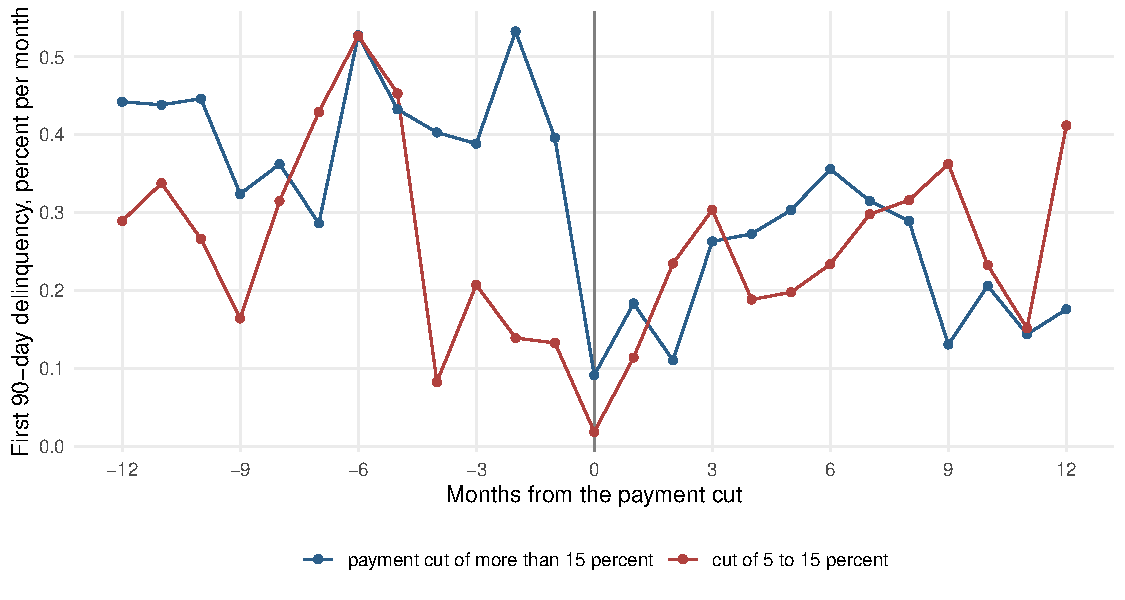
\includegraphics[width=0.85\textwidth]{figures/fig_arm_event.pdf}
\caption{First 90-day delinquency around a payment cut on a mortgage whose balance amortizes before the cut, by the size of the cut. The largest cuts reset in 2010 and 2011; the fall after month three is the calendar decline in delinquency, which the fixed effects of Table \ref{tab:arm_samples} remove.}
\label{fig:arm_event}
% replication: Code/identification/I10_arm_reset.R, Code/exhibits/make_arm_figures.R
\end{figure}

\begin{figure}[H]
\centering
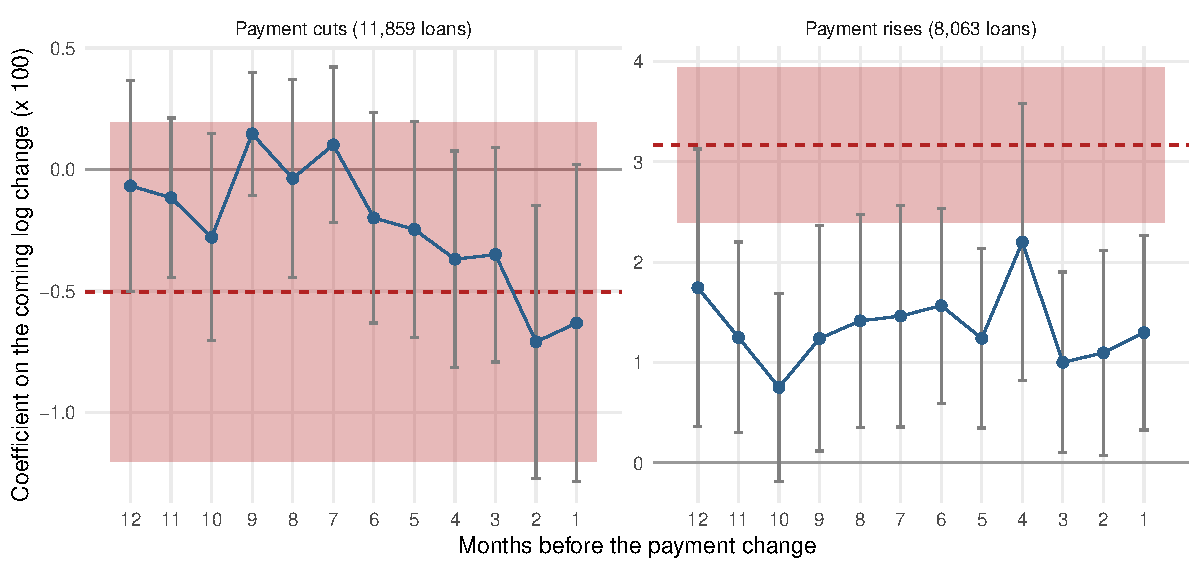
\includegraphics[width=0.95\textwidth]{figures/fig_arm_anticipation.pdf}
\caption{The response of first 90-day delinquency to the coming log payment change at each of the twelve months before it, relative to the same loan 13 to 24 months before, with 95 percent bands; the dashed line and band are the response at the change. Left: rate cuts; right: rate rises. Under Proposition \ref{prop:sensT} the response before the change has the sign of the response at it.}
\label{fig:arm_anticipation}
% replication: Code/identification/I10_arm_reset.R, Code/exhibits/make_arm_figures.R; results/arm_event_study_cut.csv, results/arm_event_classes_detail.csv
\end{figure}

\begin{table}[H]
\centering
\caption{The reset responses across samples}
\label{tab:arm_samples}
\small
\resizebox{\textwidth}{!}{\begin{tabular}{lrrrrr}
\toprule
Sample & Loans & Events & Base hazard & At the change & Before (1--4 months) \\
\midrule
All hybrid-age payment changes & 72,720 & 12,165 & 0.94 & 1.15 (0.08) & -0.99 (0.14) \\
Payment cuts of more than 15 percent & 14,101 & 2,578 & 1.36 & 0.12 (0.08) & -1.19 (0.24) \\
Rate cuts, amortising before and after & 6,114 & 361 & 0.29 & 0.37 (0.16) & -2.36 (0.49) \\
Rate cuts, amortising before & 11,859 & 1,066 & 0.42 & -0.50 (0.36) & -0.47 (0.13) \\
Rate rises, amortising before & 8,063 & 1,218 & 0.54 & 3.17 (0.40) & 1.27 (0.26) \\
\bottomrule
\end{tabular}
}
\vspace{0.5em}
\begin{minipage}{0.92\textwidth}
\noindent \small \textit{Notes:} Linear probability coefficients ($\times 100$) of first 90-day delinquency on the log payment change interacted with an indicator for months at or after the change, and the precision-weighted mean of the coefficients on the coming change at one to four months before it, with loan and origination-half-year-by-calendar-month fixed effects; standard errors clustered by lender-year. Base hazard: percent per month, 13 to 24 months before the change. Samples: all payment changes at hybrid reset ages; cuts of more than 15 percent; rate cuts of Table \ref{tab:arm_classes} with the balance amortizing before and after the cut; rate cuts with the balance amortizing before the cut and the trade open three months after it; rate rises on the same condition.
\end{minipage}
% replication: Code/identification/I10b_arm_reset_iv.R
\end{table}

% sections/student_resumption.tex: the October 2023 student-loan payment resumption as a cross-loan timing experiment (E13, I11). Numbers filled from results/student_*.csv.
\subsection{Student Loans: The Statutory Payment Resumption}\label{sec:studentloan}

\paragraph{The design in summary.} The Fiscal Responsibility Act of 3 June 2023 fixed the date on which federal student-loan payments resumed, October 2023, and the size of each bill was fixed by the student loan; for the 324,586 holders in the panel who also hold an auto loan it is a payment increase on another account at a date fixed by statute four months in advance, at an auto balance that does not change. Auto default did not respond to it at any horizon. On 743,487 auto loans with 17,711 first 90-day delinquencies, the coefficient of delinquency on the resumed bill per hundred dollars, in units of $10^{-5}$ per month with loan and calendar-month fixed effects, is $-3.1$ before the statute, $-4.1$ in the four months between the statute and the first bill and $-5.9$ from October 2023, with standard errors between $0.5$ and $1.0$; the change at the bill is $-2.8$ ($0.6$), against the $+5.9$ that an enforced payment of that size would produce at the panel's payment elasticity, and no score tercile or income quartile has a positive coefficient before the bill, at it or after it (Table \ref{tab:student_groups}). The reason is that the bill was not a payment. By January 2024, 41 percent of the holders billed up to \$100 and 61 percent of those billed more than \$500 show a positive payment, the shares do not rise afterward, and under the twelve-month on-ramp a missed payment was not reported as delinquent until October 2024, so half of the resumed bills were unpaid and had no consequence within the window (Table \ref{tab:student_takeup}). Proposition \ref{prop:sensT} weights a payment by the probability that it is due, and a bill that half of its recipients set aside is not the known and binding payment of Remark \ref{rem:experimentsT}; the measured zero, within $\pm 1.4 \times 10^{-5}$ per month, two percent of the base hazard, is the model's response to an obligation that is not enforced. Appendix \ref{appendix:timing} reports the take-up, the monthly profile and the responses by group.

Federal student-loan payments were suspended in March 2020. The Fiscal Responsibility Act of 3 June 2023 fixed the end of the suspension: interest from 1 September and the first payment due in October 2023. For a borrower who also holds an auto loan, the resumption is a payment increase on another account at a date fixed by statute four months in advance, of a size fixed by the student loan's balance and plan, at an auto balance that does not change. It is the design of Remark \ref{rem:experimentsT} at scale: the one-percent panel holds 438,311 consumers with a student-loan balance in September 2023, of whom 324,586 hold an auto loan open in January 2023, and their auto loans record 17,711 first 90-day delinquencies over 2022 to mid-2025. The response of auto delinquency to the size of the resumed payment in June to September 2023, the four months between the statute and the first bill, relative to the response from October 2023, is the anticipation profile of Proposition \ref{prop:sensT} at horizons of four to one months, $D(\tau)Q_\tau\lambda$, and the borrowers whose resumed payment is zero on a positive balance, the income-driven plans, receive the same information and no payment.

\paragraph{The exposure and its take-up.} The median of the 438,311 holders (the bins of Table \ref{tab:student_takeup} cover the 429,918 with a bill observed) owed \$20,408 in September 2023 and was billed \$80 a month from November, with an interquartile range from zero to \$244; 34 percent of holders with a positive balance were billed nothing, the income-driven plans. The bill was not a payment. Table \ref{tab:student_takeup} follows the student trades' actual-payment field: by January 2024, 41 percent of the holders billed up to \$100 and 61 percent of those billed more than \$500 show a positive payment, the median payment among those billed \$100 to \$500 equals the bill, and the shares do not rise afterward. Under the Department of Education's twelve-month on-ramp, missed payments were not reported as delinquent until October 2024, and the share of holders with a past-due student balance stays between two and four percent through January 2025. Half of the resumed bills were paid and the other half had no consequence within the window.

\paragraph{The response.} Figure \ref{fig:student_profile} reports, for each month from March 2023 to December 2025, the coefficient of first 90-day (and 60-day) auto delinquency on the resumed monthly bill in hundreds of dollars, with loan and calendar-month fixed effects and January 2022 to February 2023 as the reference, on 743,487 auto loans open in January 2023 and 17,711 first 90-day events. The coefficients, times $10^{5}$, are $-3.1$ in March to May 2023, before the statute, $-4.1$ in the four months between the statute and the first bill, $-5.9$ in October to December 2023, near $-6$ through 2024, and $-5.7$ from May 2025, when collection resumed, with standard errors between $0.5$ and $1.0$. The base hazard is $0.066$ percent per month. The response an enforced payment of the same size would produce is the panel's elasticity applied to the auto payment: a \$100 bill against a median auto payment near \$500 is a fifth of the obligation, and at the elasticity of $0.45$ the coefficient would be $+5.9$. The measured coefficient is negative at every month, is negative before the statute, and changes between the pre-statute months and the bill months by $-2.8$ ($0.6$). The sign is the composition of the exposure, not a response: a larger bill is a larger balance, which is more education and a lower and falling auto-delinquency hazard over 2023 to 2025, and the fixed effects remove the level but not the drift. Table \ref{tab:student_groups} reports the same three windows by score tercile and income quartile: no group has a positive coefficient before the bill, at it, or after it, and the bottom score tercile, with 13,837 events, has $-3$ ($1$) before and $-6$ ($2$) at the bill.

\paragraph{What the resumption establishes.} Proposition \ref{prop:sensT} weights a future payment by the probability that it is due, and a bill that half of its recipients do not pay and that has no consequence for a year is due with a probability that the design does not fix. The resumption therefore does not meet the premise of Remark \ref{rem:experimentsT}, a known and binding payment, at the enforcement margin, and its zero is the model's zero for an obligation the borrower can set aside: the response of auto default to \$100 of unenforced bill on another account is measured to within $\pm 1.4\times 10^{-5}$ per month, two percent of the base hazard, and is not positive at any horizon in any group. What remains open is the response to the enforced payments after mid-2025, which the coefficients from May to December 2025 do not distinguish from the preceding drift, and which a longer panel will measure. The two timing designs the bureau offers in this period, the resets and the resumption, are both found and both measured, and neither delivers the discount function: the resets for want of exogenous variation in size and of events, the resumption for want of an enforced payment. Appendix \ref{appendix:strategies} records both, and the discount rate the paper reports comes from the experiments of Section \ref{sec:quasi}, whose payment changes were enforced and whose sizes were assigned.

\begin{figure}[H]
\centering
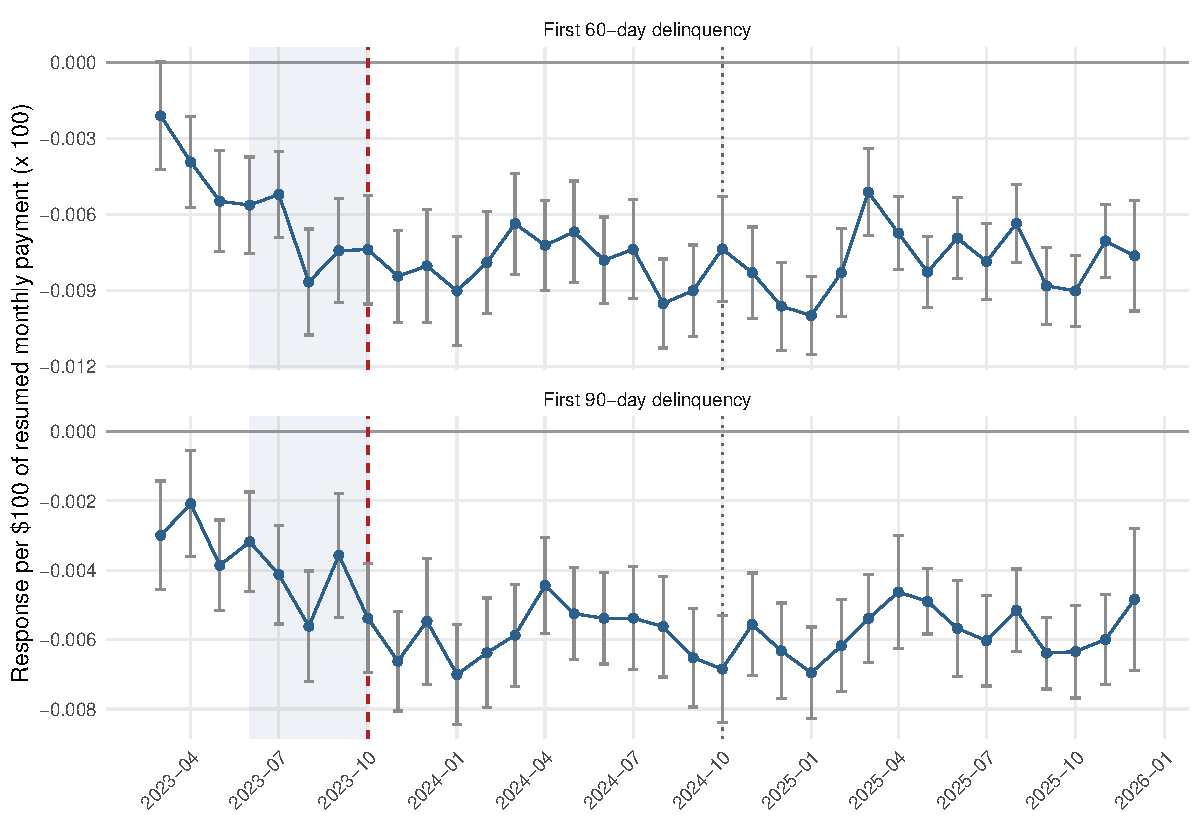
\includegraphics[width=0.95\textwidth]{figures/fig_student_profile.pdf}
\caption{Auto-loan delinquency and the resumed student-loan bill. Coefficients ($\times 100$) of first 90-day and 60-day delinquency on the resumed monthly bill in hundreds of dollars, by calendar month, with loan and month fixed effects; reference January 2022 to February 2023; 95 percent bands. Shaded: the four months between the statute of 3 June 2023 and the first bill; dashed: October 2023; dotted: the end of the on-ramp, October 2024.}
\label{fig:student_profile}
% replication: Code/extract/E13_student_resumption.R, Code/identification/I11_student_resumption.R, Code/exhibits/make_student_figures.R
\end{figure}

\begin{table}[H]
\centering
\caption{Take-up of the resumed student-loan bills}
\label{tab:student_takeup}
\small
\resizebox{\textwidth}{!}{\begin{tabular}{lrrrrrrrrr}
\toprule
Resumed bill & Holders & \multicolumn{2}{c}{2023-11} & \multicolumn{2}{c}{2024-01} & \multicolumn{2}{c}{2024-10} & \multicolumn{2}{c}{2025-01} \\
\cmidrule(lr){3-4}\cmidrule(lr){5-6}\cmidrule(lr){7-8}\cmidrule(lr){9-10}
 & (2023-09) & Paying & Past due & Paying & Past due & Paying & Past due & Paying & Past due \\
\midrule
Zero & 149,088 & 0.03 & 0.008 & 0.04 & 0.007 & 0.08 & 0.011 & 0.10 & 0.012 \\
\$1--100 & 83,372 & 0.31 & 0.019 & 0.41 & 0.018 & 0.36 & 0.017 & 0.36 & 0.019 \\
\$101--250 & 92,512 & 0.43 & 0.020 & 0.55 & 0.020 & 0.49 & 0.020 & 0.50 & 0.022 \\
\$251--500 & 61,295 & 0.50 & 0.026 & 0.60 & 0.026 & 0.55 & 0.025 & 0.55 & 0.027 \\
More than \$500 & 43,651 & 0.55 & 0.043 & 0.61 & 0.044 & 0.57 & 0.041 & 0.56 & 0.042 \\
\bottomrule
\end{tabular}
}
\vspace{0.5em}
\begin{minipage}{0.92\textwidth}
\noindent \small \textit{Notes:} Holders of a positive federal student-loan balance in September 2023, by the resumed monthly bill. Actual payment: the share with a positive actual-payment amount on any student trade in the month; ratio: the median of actual to scheduled payment among all holders in the bin; past due: the share with a positive past-due student balance.
\end{minipage}
% replication: Code/extract/E13b_student_takeup.R
\end{table}

\begin{table}[H]
\centering
\caption{The response to the resumed bill by group}
\label{tab:student_groups}
\small
\resizebox{\textwidth}{!}{\begin{tabular}{llrrrrrrr}
\toprule
Outcome & Group & Loans & Events & Base & Before (Jun--Sep 2023) & At (Oct--Dec 2023) & After (2024--25) & Ratio \\
\midrule
90-day & All  & 738,722 & 17,711 & 0.066 & -0.004 (0.000) & -0.005 (0.000) & -0.005 (0.000) & 0.68 \\
90-day & Score tercile 1 & 256,441 & 13,837 & 0.157 & -0.003 (0.001) & -0.006 (0.002) & -0.005 (0.001) & 0.62 \\
90-day & Score tercile 2 & 242,503 & 3,316 & 0.031 & -0.001 (0.001) & -0.003 (0.001) & -0.003 (0.000) & 0.50 \\
90-day & Score tercile 3 & 239,762 & 558 & 0.004 & -0.000 (0.000) & -0.001 (0.000) & -0.001 (0.000) & 0.44 \\
90-day & Income quartile 1 & 187,038 & 7,716 & 0.131 & -0.008 (0.001) & -0.009 (0.002) & -0.009 (0.001) & 0.86 \\
90-day & Income quartile 2 & 185,814 & 6,564 & 0.091 & 0.001 (0.002) & -0.006 (0.002) & -0.004 (0.001) & -0.10 \\
90-day & Income quartile 3 & 181,150 & 2,529 & 0.029 & -0.001 (0.001) & 0.001 (0.001) & -0.001 (0.000) & -0.64 \\
90-day & Income quartile 4 & 178,412 & 780 & 0.008 & -0.000 (0.000) & -0.000 (0.000) & -0.000 (0.000) & 3.50 \\
60-day & All  & 733,653 & 28,742 & 0.124 & -0.006 (0.001) & -0.007 (0.001) & -0.007 (0.000) & 0.83 \\
60-day & Score tercile 1 & 257,787 & 21,831 & 0.290 & -0.006 (0.002) & -0.005 (0.002) & -0.007 (0.001) & 1.21 \\
60-day & Score tercile 2 & 239,790 & 5,795 & 0.060 & -0.003 (0.001) & -0.005 (0.001) & -0.005 (0.000) & 0.57 \\
60-day & Score tercile 3 & 236,060 & 1,116 & 0.010 & -0.000 (0.000) & -0.001 (0.000) & -0.001 (0.000) & 0.24 \\
60-day & Income quartile 1 & 186,638 & 11,463 & 0.222 & -0.010 (0.002) & -0.010 (0.002) & -0.013 (0.001) & 0.97 \\
60-day & Income quartile 2 & 185,493 & 10,807 & 0.179 & -0.005 (0.002) & -0.006 (0.002) & -0.005 (0.001) & 0.92 \\
60-day & Income quartile 3 & 179,410 & 4,661 & 0.066 & 0.001 (0.001) & -0.001 (0.001) & -0.001 (0.001) & -0.60 \\
60-day & Income quartile 4 & 175,861 & 1,652 & 0.020 & -0.001 (0.000) & -0.001 (0.000) & -0.001 (0.000) & 0.44 \\
\bottomrule
\end{tabular}
}
\vspace{0.5em}
\begin{minipage}{0.92\textwidth}
\noindent \small \textit{Notes:} Coefficients ($\times 100$) of first delinquency on the resumed bill in hundreds of dollars interacted with three windows, June to September 2023 (before the first bill), October to December 2023 (at it) and January 2024 onward (after it), with loan and calendar-month fixed effects; standard errors clustered by consumer; base: the monthly hazard in the reference window, percent. Ratio: before over at. Score and income at the auto loan's first sight in the panel.
\end{minipage}
% replication: Code/identification/I11_student_resumption.R
\end{table}




\section{Additional Figures and Tables}\label{appendix:figures}

Figure \ref{fig:origination_volume} shows the auto panel's origination volumes by cohort (Section \ref{sec:data}); Table \ref{tab:rho_within_states} and Figure \ref{fig:rho_within} the rate from the within-borrower design with the states (Section \ref{sec:rate_people}); Table \ref{tab:liquidity} the liquidity diagnostics (Section \ref{sec:liquidity}); Table \ref{tab:exposure} the payment elasticity by group for four windows and Figure \ref{fig:exposure_geo} the power-preserving splits of the payment margin (Section \ref{sec:exposure}); Figure \ref{fig:geo_politics} the payment elasticity and the term-to-payment ratio by state against the presidential vote (Appendix \ref{appendix:traits}).

\begin{figure}[H]
    \centering
    \caption{Auto loans by origination cohort}
    \label{fig:origination_volume}
    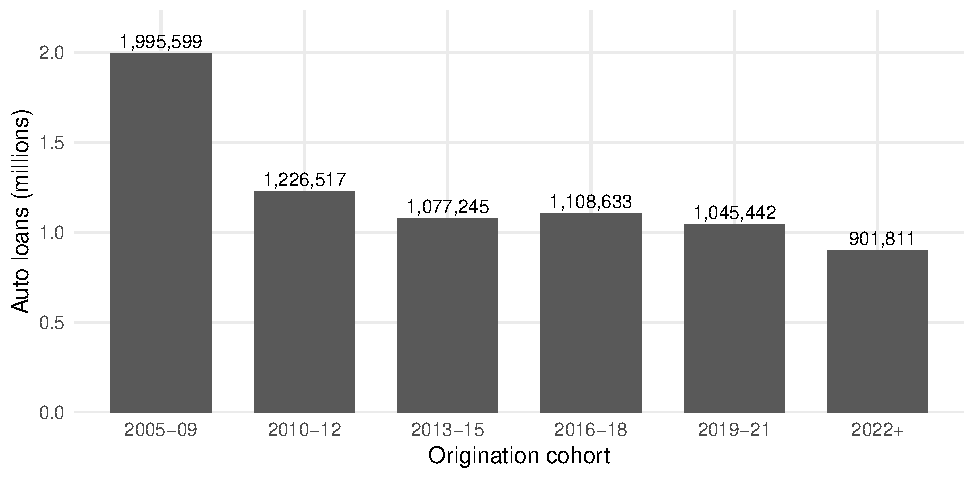
\includegraphics[width=0.8\textwidth]{figures/fig_loans_by_cohort.pdf}
    \small Notes: Number of auto loans in the one-percent credit-bureau panel's windows sample, by origination cohort.
% replication: Code/exhibits/make_panel_figures.R; results/panel_windows_auto.csv
\end{figure}

\begin{figure}[ht]
\centering
% figures/fig_design_map.tex: the designs, the inputs each supplies to the formula, and the outputs (TikZ; no data).
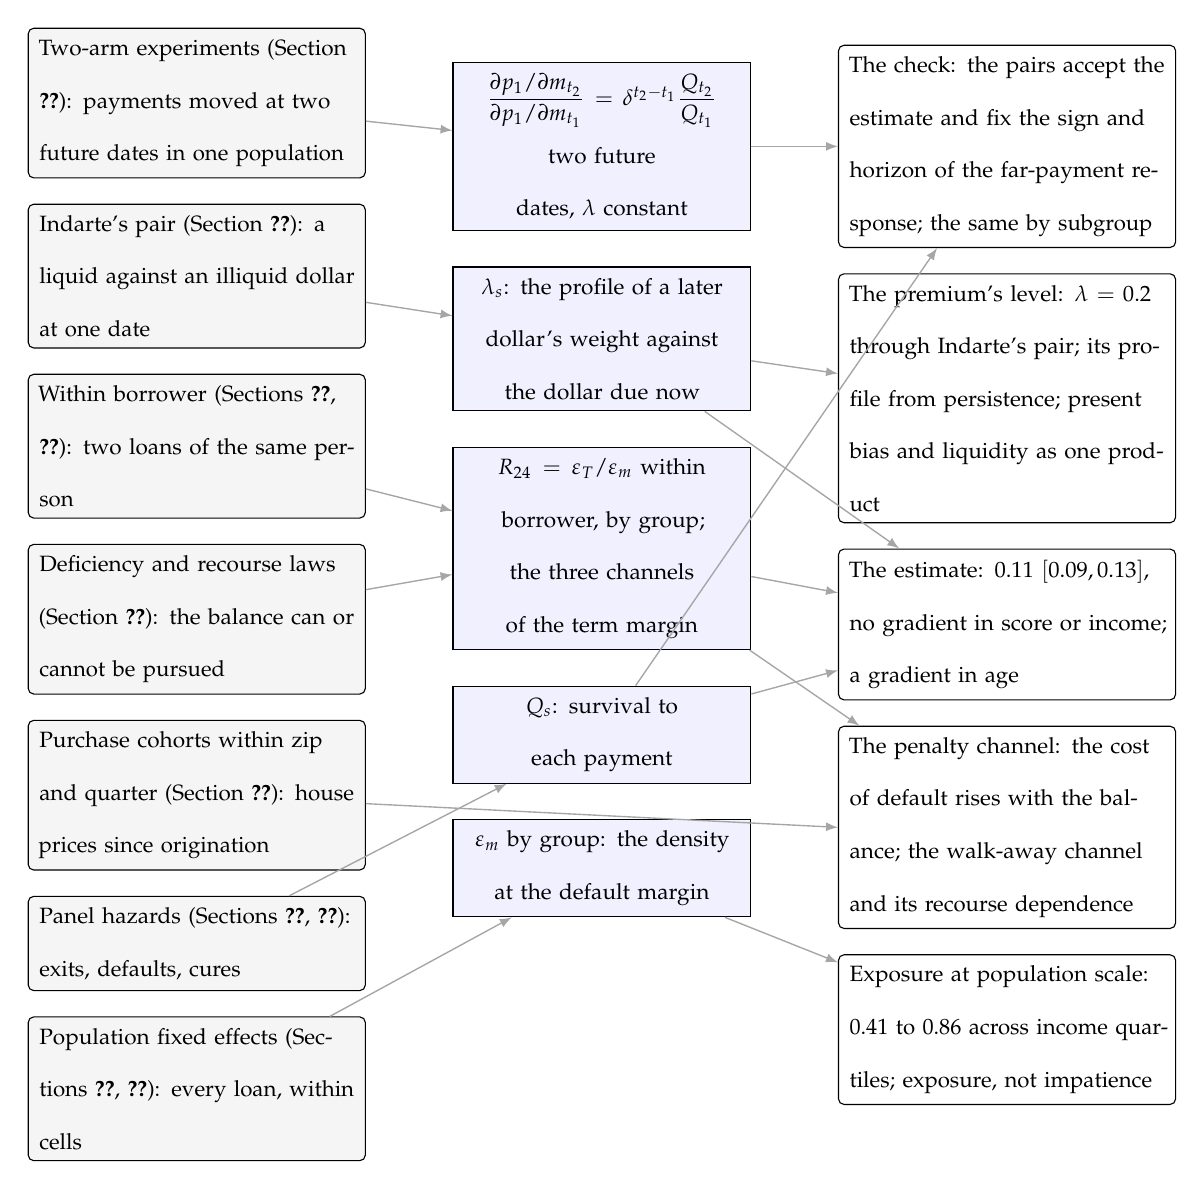
\begin{tikzpicture}[
  font=\footnotesize,
  design/.style={rectangle, draw, rounded corners=2pt, fill=gray!8, text width=4.0cm, align=left, inner sep=4pt, minimum height=0.9cm},
  input/.style={rectangle, draw, fill=blue!6, text width=3.5cm, align=center, inner sep=4pt, minimum height=0.9cm},
  output/.style={rectangle, draw, rounded corners=2pt, fill=white, text width=4.0cm, align=left, inner sep=4pt, minimum height=0.9cm},
  arr/.style={-latex, gray!70, line width=0.5pt},
  node distance=0.32cm and 1.1cm]
\node[design] (d1) {Two-arm experiments (Section \ref{sec:quasi}): payments moved at two future dates in one population};
\node[design, below=of d1] (d2) {Indarte's pair (Section \ref{sec:quasi}): a liquid against an illiquid dollar at one date};
\node[design, below=of d2] (d3) {Within borrower (Sections \ref{sec:rate_people}, \ref{sec:termmargin}): two loans of the same person};
\node[design, below=of d3] (d4) {Deficiency and recourse laws (Section \ref{sec:termmargin}): the balance can or cannot be pursued};
\node[design, below=of d4] (d5) {Purchase cohorts within zip and quarter (Section \ref{sec:equity}): house prices since origination};
\node[design, below=of d5] (d6) {Panel hazards (Sections \ref{sec:data}, \ref{sec:mapping}): exits, defaults, cures};
\node[design, below=of d6] (d7) {Population fixed effects (Sections \ref{sec:identification}, \ref{sec:heterogeneity}): every loan, within cells};
\node[input, right=of d1.east, yshift=-0.55cm] (i1) {$\dfrac{\partial p_1/\partial m_{t_2}}{\partial p_1/\partial m_{t_1}} = \delta^{t_2-t_1}\dfrac{Q_{t_2}}{Q_{t_1}}$ \\[2pt] two future dates, $\lambda$ constant};
\node[input, below=0.45cm of i1] (i2) {$\lambda_s$: the profile of a later dollar's weight against the dollar due now};
\node[input, below=0.45cm of i2] (i3) {$R_{24} = \varepsilon_T/\varepsilon_m$ within borrower, by group; the three channels of the term margin};
\node[input, below=0.45cm of i3] (i4) {$Q_s$: survival to each payment};
\node[input, below=0.45cm of i4] (i5) {$\varepsilon_m$ by group: the density at the default margin};
\node[output, right=of i1] (o1) {The check: the pairs accept the estimate and fix the sign and horizon of the far-payment response; the same by subgroup};
\node[output, below=of o1] (o2) {The premium's level: $\lambda = 0.2$ through Indarte's pair; its profile from persistence; present bias and liquidity as one product};
\node[output, below=of o2] (o3) {The estimate: $0.11$ $[0.09, 0.13]$, no gradient in score or income; a gradient in age};
\node[output, below=of o3] (o4) {The penalty channel: the cost of default rises with the balance; the walk-away channel and its recourse dependence};
\node[output, below=of o4] (o5) {Exposure at population scale: $0.41$ to $0.86$ across income quartiles; exposure, not impatience};
\draw[arr] (d1) -- (i1); \draw[arr] (d2) -- (i2); \draw[arr] (d3) -- (i3); \draw[arr] (d4) -- (i3); \draw[arr] (d5) -- (o4.west);
\draw[arr] (d6) -- (i4); \draw[arr] (d7) -- (i5);
\draw[arr] (i1) -- (o1); \draw[arr] (i2) -- (o2); \draw[arr] (i2) -- (o3); \draw[arr] (i3) -- (o3); \draw[arr] (i3) -- (o4); \draw[arr] (i4) -- (o1); \draw[arr] (i4) -- (o3); \draw[arr] (i5) -- (o5);
\end{tikzpicture}

\caption{From designs to inputs to outputs. Left: each identification design and the section that reports it. Middle: the object it supplies to the formula of equation \eqref{eq:weights}. Right: the results that rest on it.}
\label{fig:design_map}
% replication: Draft/figures/fig_design_map.tex (a diagram; no data)
\end{figure}

\begin{figure}[ht]
\centering
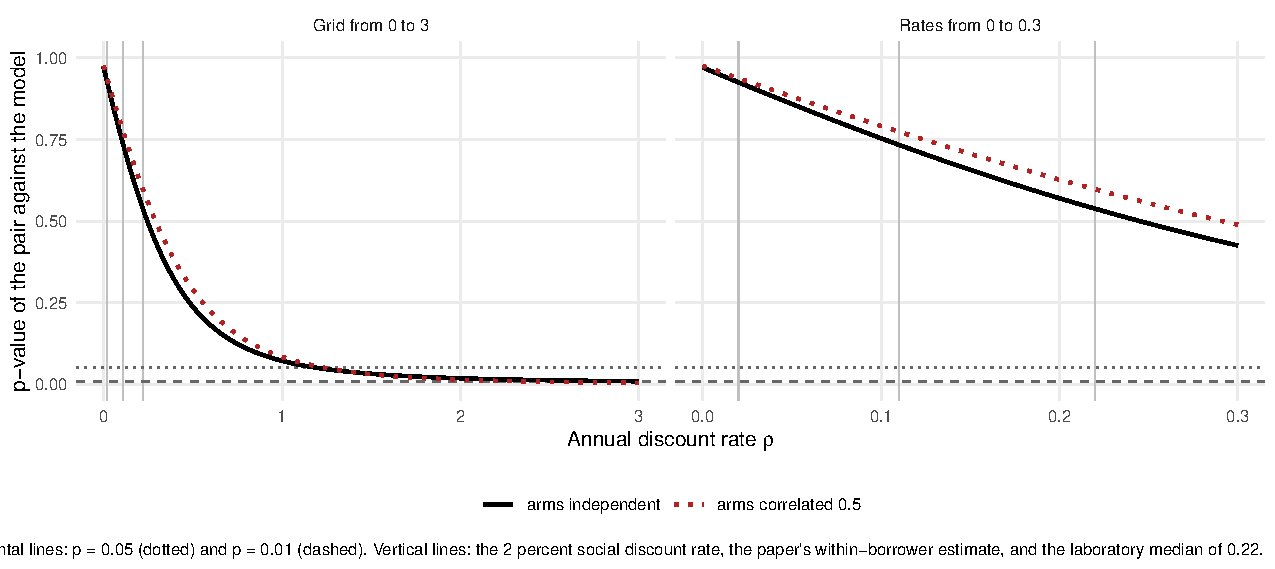
\includegraphics[width=\textwidth]{figures/fig_ds_pvalue.pdf}
\caption{The Dobbie--Song pair against the model on the grid of the annual rate. Each curve is the $p$-value of the joint test of the write-down and payment-reduction effects against the model's line, aggregated over the study's five-year window as in equation \eqref{eq:window} at the marginal-utility profile, with survival from the study's own exit hazards: with the two arms independent (solid) and with their sampling errors correlated at $0.5$ (dotted). The right panel repeats the left on rates from 0 to 0.3.}
\label{fig:ds_pvalue}
% replication: Code/local/experiments_ledger.R, Code/exhibits/make_ds_pvalue_figure.R
\end{figure}

\begin{table}[H]
\centering
\caption{The rate from the within-borrower design, with the twelve largest states}
\label{tab:rho_within_states}
\small
\resizebox{\textwidth}{!}{\begin{tabular}{llrrrrrrr}
\toprule
Dimension & Group & Loans & $R_{24}$ (s.e.) & $\lambda_{2}$ & $\lambda_{60}$ & $h$ & $\rho$ & 95\% set \\
\midrule
All &  & 59,155,190 & 0.55 (0.01) & 0.89 & 0.35 & 0.19 & 0.02 & [0.01, 0.04] \\
\midrule
Score decile & 1 & 5,754,666 & 0.53 (0.03) & 0.89 & 0.40 & 0.13 & 0.14 & [0.10, 0.18] \\
Score decile & 2 & 5,784,547 & 0.50 (0.02) & 0.89 & 0.39 & 0.17 & 0.11 & [0.08, 0.16] \\
Score decile & 3 & 5,819,449 & 0.47 (0.02) & 0.89 & 0.37 & 0.19 & 0.10 & [0.06, 0.14] \\
Score decile & 4 & 5,837,786 & 0.44 (0.02) & 0.89 & 0.36 & 0.20 & 0.11 & [0.07, 0.16] \\
Score decile & 5 & 5,840,925 & 0.37 (0.03) & 0.89 & 0.34 & 0.20 & 0.17 & [0.12, 0.23] \\
Score decile & 6 & 5,895,688 & 0.32 (0.03) & 0.88 & 0.32 & 0.20 & 0.22 & [0.15, 0.29] \\
Score decile & 7 & 5,958,258 & 0.39 (0.04) & 0.88 & 0.31 & 0.21 & 0.12 & [0.06, 0.20] \\
Score decile & 8 & 6,024,937 & 0.40 (0.04) & 0.88 & 0.29 & 0.21 & 0.10 & [0.02, 0.19] \\
Score decile & 9 & 6,094,315 & 0.44 (0.06) & 0.88 & 0.28 & 0.21 & 0.05 & [0.00, 0.18] \\
Score decile & 10 & 6,144,619 & 0.49 (0.10) & 0.88 & 0.26 & 0.20 & 0.01 & [0.00, 0.19] \\
\midrule
Score tercile & 1 & 19,305,393 & 0.49 (0.01) & 0.89 & 0.39 & 0.17 & 0.11 & [0.09, 0.13] \\
Score tercile & 2 & 19,593,019 & 0.39 (0.02) & 0.88 & 0.34 & 0.21 & 0.15 & [0.12, 0.18] \\
Score tercile & 3 & 20,256,778 & 0.45 (0.03) & 0.88 & 0.28 & 0.20 & 0.06 & [0.01, 0.11] \\
\midrule
Income quartile & 1 & 1,417,320 & 0.34 (0.05) & 0.89 & 0.38 & 0.18 & 0.24 & [0.15, 0.36] \\
Income quartile & 2 & 1,464,021 & 0.52 (0.05) & 0.89 & 0.37 & 0.19 & 0.06 & [0.00, 0.15] \\
Income quartile & 3 & 1,507,500 & 0.45 (0.07) & 0.88 & 0.32 & 0.21 & 0.08 & [0.00, 0.21] \\
Income quartile & 4 & 1,525,715 & 0.27 (0.12) & 0.88 & 0.29 & 0.20 & 0.26 & [0.02, 0.92] \\
\midrule
Age & 18-30 & 1,973,515 & 0.26 (0.05) & 0.89 & 0.36 & 0.19 & 0.32 & [0.21, 0.48] \\
Age & 31-40 & 1,390,019 & 0.62 (0.08) & 0.89 & 0.35 & 0.19 & 0.00 & [0.00, 0.10] \\
Age & 41-50 & 1,261,134 & 0.70 (0.08) & 0.88 & 0.34 & 0.19 & 0.00 & [0.00, 0.03] \\
Age & 51-60 & 805,083 & 0.75 (0.08) & 0.88 & 0.33 & 0.19 & 0.00 & [0.00, 0.00] \\
Age & 61+ & 408,746 & 0.65 (0.08) & 0.89 & 0.34 & 0.19 & 0.00 & [0.00, 0.07] \\
\midrule
Origination period & 2005-09 & 18,354,127 & 0.75 (0.02) & 0.89 & 0.36 & 0.19 & 0.00 & [0.00, 0.00] \\
Origination period & 2010-13 & 13,962,572 & 0.59 (0.02) & 0.88 & 0.34 & 0.19 & 0.00 & [0.00, 0.02] \\
Origination period & 2014-17 & 13,561,755 & 0.54 (0.02) & 0.89 & 0.36 & 0.19 & 0.04 & [0.02, 0.06] \\
Origination period & 2018-19 & 6,448,974 & 0.38 (0.02) & 0.89 & 0.35 & 0.19 & 0.18 & [0.14, 0.22] \\
Origination period & 2020-22 & 6,827,762 & -0.05 (0.03) & 0.89 & 0.35 & 0.19 & -- & [--, --] \\
State & CA & 5,609,684 & -0.21 (0.03) & 0.89 & 0.36 & 0.19 & -- & [--, --] \\
State & FL & 4,448,685 & 0.46 (0.03) & 0.89 & 0.36 & 0.19 & 0.10 & [0.05, 0.16] \\
State & GA & 1,894,594 & 0.94 (0.08) & 0.89 & 0.37 & 0.19 & 0.00 & [0.00, 0.00] \\
State & IL & 2,023,957 & 0.63 (0.07) & 0.89 & 0.35 & 0.19 & 0.00 & [0.00, 0.07] \\
State & MI & 1,939,342 & 0.54 (0.05) & 0.88 & 0.33 & 0.19 & 0.02 & [0.00, 0.10] \\
State & NC & 2,072,616 & 0.86 (0.06) & 0.89 & 0.37 & 0.19 & 0.00 & [0.00, 0.00] \\
State & NJ & 1,450,438 & 0.34 (0.07) & 0.88 & 0.34 & 0.19 & 0.21 & [0.08, 0.39] \\
State & NY & 2,727,838 & 0.36 (0.04) & 0.88 & 0.33 & 0.19 & 0.18 & [0.11, 0.28] \\
State & OH & 2,266,913 & 0.75 (0.06) & 0.89 & 0.35 & 0.19 & 0.00 & [0.00, 0.00] \\
State & PA & 2,344,897 & 0.40 (0.05) & 0.88 & 0.34 & 0.19 & 0.14 & [0.05, 0.26] \\
State & TX & 5,794,675 & 1.20 (0.04) & 0.89 & 0.36 & 0.19 & 0.00 & [0.00, 0.00] \\
State & VA & 1,556,937 & 1.00 (0.09) & 0.89 & 0.35 & 0.19 & 0.00 & [0.00, 0.00] \\
\bottomrule
\end{tabular}
}
\vspace{0.5em}
\begin{minipage}{0.92\textwidth}
\noindent \small \textit{Notes:} As Table \ref{tab:rho_within}, with the twelve largest states by loans in the design.
\end{minipage}
% replication: Code/local/within_reading.R
\end{table}

\begin{figure}[H]
\centering

\includegraphics[width=0.95\textwidth]{figures/fig_rho_within.pdf}
\caption{The rate by score decile, income quartile, age, origination period and state (the twelve largest) from the within-borrower ratio, with 95 percent sets; the dashed line is the loan-weighted decile mean, $0.11$. Rates above one are shown at one; a group whose term response is negative has no rate and is omitted.}
\label{fig:rho_within}
% replication: Code/local/within_reading.R
\end{figure}

\begin{table}[H]
\centering
\caption{Default as a portfolio choice, and the payment margin across local labor-market shocks}
\label{tab:liquidity}
\begin{tabular}{lcccc}
\toprule
\multicolumn{5}{l}{\emph{Panel A: other tradelines of auto defaulters
(measured at six months after chargeoff)}} \\
\midrule
Defaulters with other open, clean trades at default & \multicolumn{4}{r}{2,462,105} \\
Mean number of other tradelines & \multicolumn{4}{r}{10.7} \\
Share still paying at least one other trade & \multicolumn{4}{r}{65.1\%} \\
Share with all other trades current & \multicolumn{4}{r}{13.6\%} \\
Share with any other chargeoff & \multicolumn{4}{r}{22.7\%} \\
Share defaulting on every other trade & \multicolumn{4}{r}{1.6\%} \\
\midrule
\multicolumn{5}{l}{\emph{Panel B: the payment margin across local labor-market shocks (default within twelve months)}} \\
 & mean $\Delta u$ (pp) & elasticity to $m$ & (s.e.) & defaults \\
\midrule
Unemployment-change tercile 1 & -1.46 & 0.53 & (0.04) & 23,353 \\
Unemployment-change tercile 2 & -0.50 & 0.62 & (0.05) & 23,577 \\
Unemployment-change tercile 3 & +0.88 & 0.61 & (0.05) & 23,206 \\
\addlinespace
Expansion cohorts & -0.37 & 0.57 & (0.03) & 62,165 \\
Recession cohorts & -0.27 & 0.52 & (0.07) & 7,971 \\
\bottomrule
\end{tabular}

\vspace{0.5em}
\begin{minipage}{0.92\textwidth}
\noindent \small \textit{Notes:} Panel A follows every auto defaulter holding at least one other open tradeline with no charge-off at the default event, and measures the status of those other tradelines at the archive snapshot nearest six months after the charge-off; a tradeline is paying if its last-payment date falls within three months of the snapshot. Panel B estimates the payment margin (logit of default within twelve months on the log payment and log contract length within zip3-by-year cells, on the ten-percent extract) within terciles of the change in state unemployment over the loan's first eighteen months, terciles taken within origination year, and separately for recession-year origination cohorts (2007--2009, 2020).
\end{minipage}
% replication: Code/extract/E3_cross_loan.R, Code/level/L3_liquidity_shocks.R, Code/exhibits/make_summary_tables.R
\end{table}

\begin{figure}[ht]
\centering
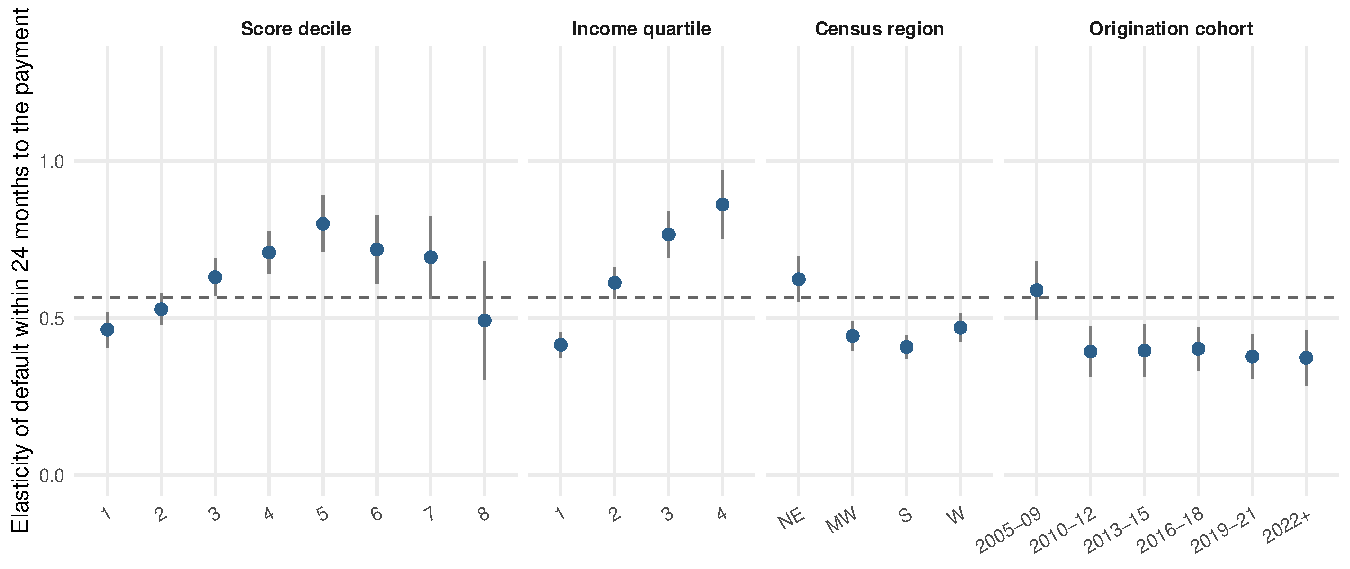
\includegraphics[width=\textwidth]{figures/fig_exposure_groups.pdf}
\caption{The payment margin across people, places and cohorts. Elasticity of charge-off within 24 months to the monthly payment from equation \eqref{eq:main_reg} within each group on the auto panel, with 95 percent bands; the dashed line is the within-borrower estimate.}
\label{fig:exposure_groups}
% replication: Code/type/T1l_windows_panel.R, Code/exhibits/make_exposure_figures.R
\end{figure}

\begin{table}[H]
\centering
\caption{The payment elasticity by group and exposure window}
\label{tab:exposure}
\small
\resizebox{\textwidth}{!}{\begin{tabular}{llcccc rr}
\toprule
 & & \multicolumn{4}{c}{Elasticity of default to the payment} & \multicolumn{2}{c}{Within 24 months} \\
\cmidrule(lr){3-6}\cmidrule(lr){7-8}
Dimension & Group & 12 months & 24 months & 36 months & Life & Defaults & Rate (\%) \\
\midrule
All loans &  & 0.45 (0.02) & 0.45 (0.02) & 0.45 (0.02) & 0.35 (0.01) & 129,722 & 1.86 \\
\addlinespace
Score tercile & 1 & 0.48 (0.03) & 0.48 (0.02) & 0.49 (0.02) & 0.37 (0.01) & 110,801 & 4.74 \\
 & 2 & 0.79 (0.04) & 0.71 (0.03) & 0.66 (0.03) & 0.55 (0.02) & 16,912 & 0.72 \\
 & 3 & 0.47 (0.09) & 0.47 (0.05) & 0.49 (0.05) & 0.33 (0.03) & 2,009 & 0.09 \\
\addlinespace
Income quartile & 1 & 0.45 (0.03) & 0.41 (0.02) & 0.42 (0.02) & 0.33 (0.01) & 85,626 & 4.94 \\
 & 2 & 0.57 (0.03) & 0.61 (0.03) & 0.59 (0.02) & 0.44 (0.02) & 31,498 & 1.78 \\
 & 3 & 0.82 (0.06) & 0.77 (0.04) & 0.74 (0.04) & 0.55 (0.02) & 9,302 & 0.53 \\
 & 4 & 0.74 (0.08) & 0.86 (0.05) & 0.79 (0.05) & 0.60 (0.03) & 3,296 & 0.19 \\
\addlinespace
Census region & NE & 0.67 (0.05) & 0.62 (0.04) & 0.61 (0.03) & 0.48 (0.02) & 13,793 & 1.25 \\
 & MW & 0.50 (0.03) & 0.44 (0.02) & 0.46 (0.02) & 0.35 (0.02) & 21,700 & 1.43 \\
 & S & 0.39 (0.02) & 0.41 (0.02) & 0.41 (0.02) & 0.31 (0.01) & 67,017 & 2.40 \\
 & W & 0.49 (0.03) & 0.47 (0.02) & 0.46 (0.02) & 0.37 (0.02) & 26,626 & 1.77 \\
\addlinespace
Origination cohort & 2005-09 & 0.54 (0.06) & 0.59 (0.05) & 0.58 (0.04) & 0.41 (0.03) & 24,610 & 1.25 \\
 & 2010-12 & 0.38 (0.05) & 0.39 (0.04) & 0.41 (0.04) & 0.30 (0.03) & 14,946 & 1.24 \\
 & 2013-15 & 0.41 (0.06) & 0.40 (0.04) & 0.38 (0.04) & 0.31 (0.03) & 25,554 & 2.40 \\
 & 2016-18 & 0.44 (0.05) & 0.40 (0.04) & 0.39 (0.03) & 0.32 (0.03) & 26,623 & 2.42 \\
 & 2019-21 & 0.38 (0.05) & 0.38 (0.04) & 0.39 (0.04) & 0.35 (0.03) & 19,715 & 1.90 \\
 & 2022+ & 0.39 (0.04) & 0.37 (0.05) & 0.36 (0.05) & 0.34 (0.04) & 18,274 & 3.07 \\
\bottomrule
\end{tabular}
}
\vspace{0.5em}
\begin{minipage}{0.92\textwidth}
\noindent \small \textit{Notes:} Elasticity of the charge-off rate within the stated window with respect to the monthly payment, equation \eqref{eq:main_reg} within each group on the auto panel; standard errors clustered by lender-year.
\end{minipage}
% replication: Code/type/T1l_windows_panel.R, Code/exhibits/make_exposure_figures.R
\end{table}

\begin{figure}[H]
\centering
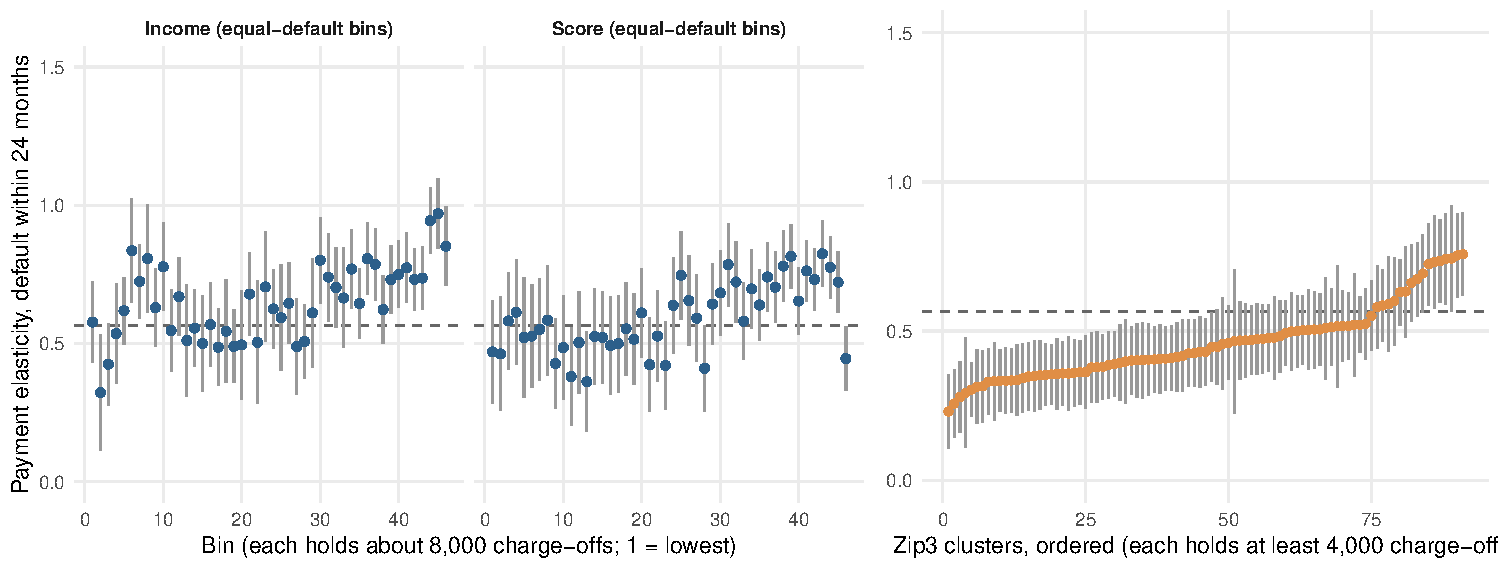
\includegraphics[width=\textwidth]{figures/fig_exposure_geo.pdf}
\caption{Power-preserving splits. Left: the payment elasticity within 24 months by equal-default bins of the score and of income. Right: the same by 91 clusters of three-digit zip codes, each holding 1,400 to 7,700 charge-offs over the life of the loan, ordered by the estimate.}
\label{fig:exposure_geo}
% replication: Code/type/T1l_windows_panel.R, Code/exhibits/make_exposure_figures.R
\end{figure}

\begin{table}[H]
\centering
\caption{The population design beside the within-borrower design, by state and by area}
\label{tab:het_geo}
\scriptsize
\resizebox{\textwidth}{!}{\begin{tabular}{llrrrrrrr}
\toprule
\multicolumn{9}{l}{\textit{Panel A: the twelve largest states by loans}} \\
 & & & Default & Exposure & Ratio & \multicolumn{2}{c}{Population rate} & Within-borrower \\
\cmidrule(lr){7-8}
Dimension & State & Loans & rate (\%) & $\varepsilon_m$ (s.e.) & $R$ (s.e.) & raw & selection-adjusted & rate \\
\midrule
State & CA & 705,223 & 1.87 & 0.54 (0.03) & 0.24 (0.10) & 0.36 [0.13, 0.99] & -- & -- \\
 & TX & 659,154 & 2.53 & 0.38 (0.02) & 0.07 (0.10) & 0.79 [0.32, $\infty$] & 0.00 [0.00, 0.07] & 0.00 [0.00, 0.00] \\
 & FL & 491,080 & 2.39 & 0.53 (0.03) & 0.14 (0.09) & 0.55 [0.24, $\infty$] & 0.60 [0.24, $\infty$] & 0.10 [0.05, 0.16] \\
 & NY & 345,971 & 1.20 & 0.68 (0.05) & 0.67 (0.16) & 0.00 [0.00, 0.19] & 2.02 [0.23, $\infty$] & 0.18 [0.11, 0.28] \\
 & PA & 280,675 & 1.36 & 0.43 (0.04) & 0.82 (0.20) & 0.00 [0.00, 0.12] & 0.20 [0.00, $\infty$] & 0.14 [0.05, 0.26] \\
 & OH & 269,949 & 1.76 & 0.42 (0.04) & 0.19 (0.16) & 0.43 [0.06, $\infty$] & 0.00 [0.00, 0.29] & 0.00 [0.00, 0.00] \\
 & IL & 252,810 & 1.63 & 0.50 (0.04) & 0.21 (0.15) & 0.40 [0.07, $\infty$] & 0.22 [0.00, 3.82] & 0.00 [0.00, 0.07] \\
 & NC & 233,451 & 2.61 & 0.34 (0.03) & 0.27 (0.16) & 0.32 [0.01, $\infty$] & 0.00 [0.00, 0.00] & 0.00 [0.00, 0.00] \\
 & MI & 229,853 & 1.19 & 0.50 (0.05) & 0.49 (0.18) & 0.06 [0.00, 0.51] & 0.00 [0.00, 0.27] & 0.02 [0.00, 0.10] \\
 & GA & 218,582 & 2.93 & 0.43 (0.03) & -0.16 (0.13) & -- & 0.10 [0.00, 0.49] & 0.00 [0.00, 0.00] \\
 & VA & 186,112 & 1.57 & 0.44 (0.04) & -0.03 (0.19) & -- & 0.00 [0.00, 0.25] & 0.00 [0.00, 0.00] \\
 & NJ & 179,254 & 1.24 & 0.70 (0.07) & 0.59 (0.18) & 0.00 [0.00, 0.35] & -- & 0.21 [0.08, 0.39] \\
\midrule
\multicolumn{9}{l}{\textit{Panel B: the 91 equal-default zip3 clusters by decile of exposure}} \\
Decile & Clusters & Loans & rate (\%) & $\varepsilon_m$, range & mean $R$ (s.e.) & rate at the mean $R$ & & \\
\midrule
1 & 9 & 601,460 & 2.29 & 0.23--0.33 & 0.35 (0.13) & 0.20 [0.00, 0.66] & & \\
2 & 9 & 559,429 & 2.48 & 0.33--0.35 & 0.01 (0.10) & 1.41 [0.40, $\infty$] & & \\
3 & 9 & 685,533 & 1.87 & 0.35--0.38 & 0.22 (0.10) & 0.38 [0.13, 1.20] & & \\
4 & 9 & 651,876 & 1.89 & 0.38--0.40 & 0.11 (0.09) & 0.62 [0.27, $\infty$] & & \\
5 & 9 & 775,885 & 1.82 & 0.40--0.43 & 0.10 (0.09) & 0.67 [0.31, $\infty$] & & \\
6 & 9 & 691,880 & 1.72 & 0.43--0.47 & 0.11 (0.09) & 0.63 [0.29, $\infty$] & & \\
7 & 9 & 707,643 & 1.90 & 0.47--0.50 & -0.01 (0.07) & -- & & \\
8 & 9 & 638,674 & 1.76 & 0.50--0.52 & 0.34 (0.08) & 0.22 [0.07, 0.46] & & \\
9 & 9 & 821,212 & 1.62 & 0.52--0.63 & 0.43 (0.07) & 0.13 [0.02, 0.28] & & \\
10 & 10 & 838,374 & 1.53 & 0.66--0.76 & 0.40 (0.06) & 0.15 [0.05, 0.29] & & \\
\bottomrule
\end{tabular}
}
\vspace{0.5em}
\begin{minipage}{0.95\textwidth}
\noindent \small \textit{Notes:} As Table \ref{tab:het_population}. Panel A: the twelve largest states by loans. Panel B: the 91 equal-default clusters of three-digit zip codes, each holding 1,400 to 7,700 charge-offs over the life of the loan, grouped into deciles of exposure; the ratio is the loan-weighted mean over the decile's clusters and its rate is mapped with the pooled profile and exit hazard. Every state is in \texttt{results/heterogeneity\_population.csv}.
\end{minipage}
% replication: Code/type/T1l_windows_panel.R, Code/local/heterogeneity_population.R, Code/exhibits/make_heterogeneity_tables.R; results/heterogeneity_population.csv
\end{table}

\begin{figure}[ht]
\centering
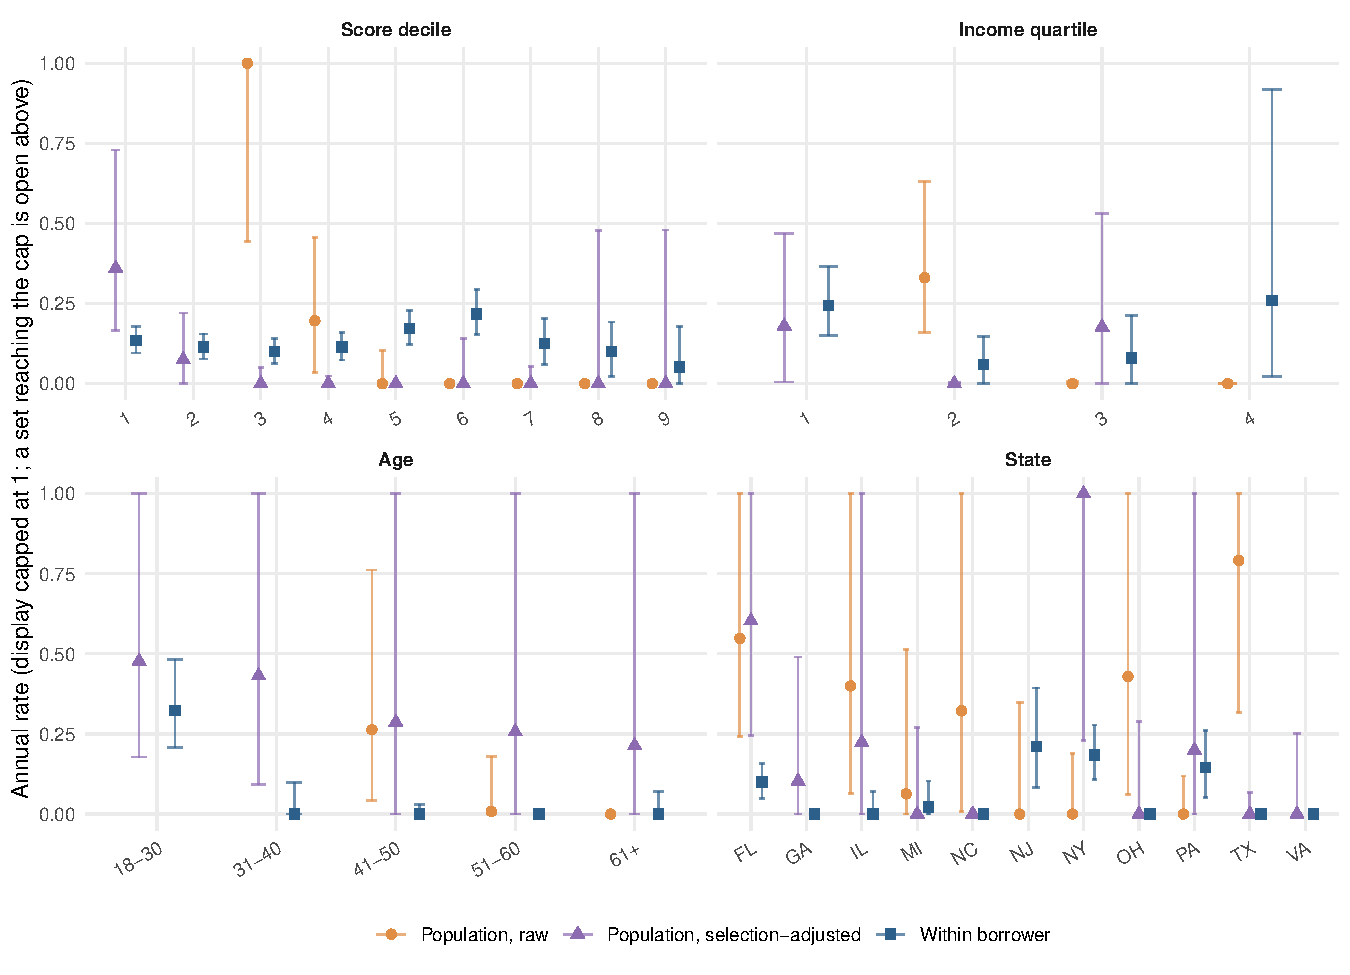
\includegraphics[width=\textwidth]{figures/fig_het_agreement.pdf}
\caption{The population rate, raw and selection-adjusted, and the within-borrower rate, with 95 percent sets, by score decile, income quartile and the twelve largest states (Tables \ref{tab:het_population} and \ref{tab:het_geo}). Rates above the display cap are shown at the cap; an open set ends at the cap.}
\label{fig:het_agreement}
% replication: Code/local/heterogeneity_population.R, Code/exhibits/make_heterogeneity_tables.R; results/heterogeneity_population.csv
\end{figure}

\begin{figure}[H]
\centering
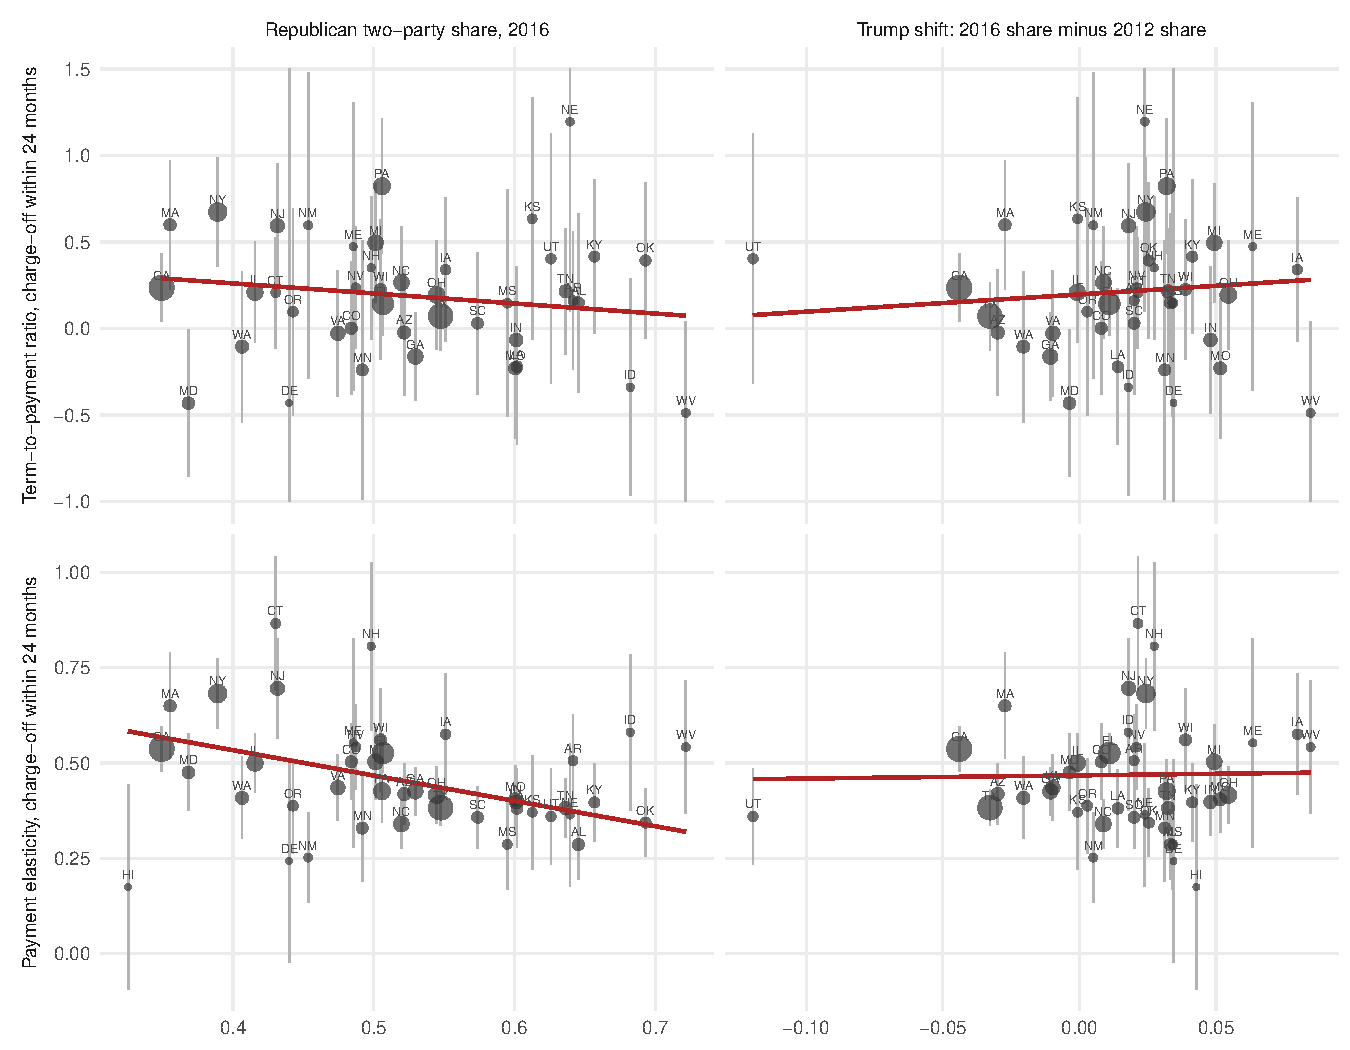
\includegraphics[width=\textwidth]{figures/fig_geo_politics.pdf}
\caption{The term-to-payment ratio and the payment elasticity by state against the vote. Charge-off within 24 months on the auto panel, states with at least 300 charge-offs; points are scaled by loans, bars are 95 percent intervals (delta method for the ratio), lines are loans-weighted fits. Left: the Republican two-party share of the 2016 presidential vote; right: the 2016 share minus the 2012 share. Hawaii (ratio $-2.0$, standard error $2.4$) lies outside the range of the upper panels.}
\label{fig:geo_politics}
% replication: Code/local/geo_politics_v2.R
\end{figure}

\begin{figure}[ht]
\centering
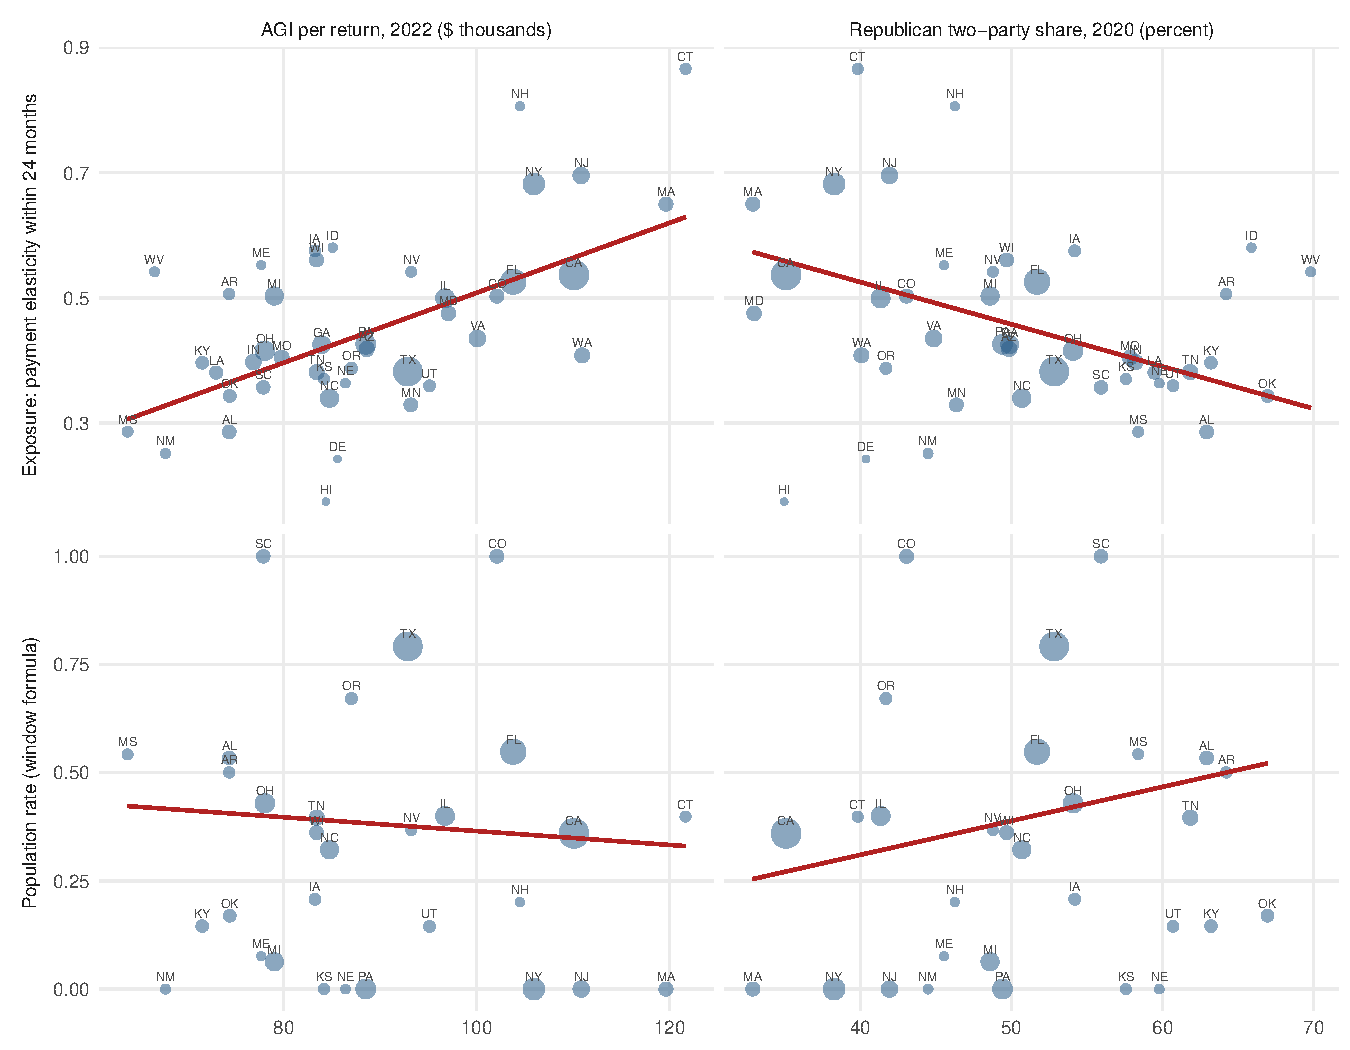
\includegraphics[width=\textwidth]{figures/fig_geo_correlates.pdf}
\caption{Exposure (upper row) and the population rate (lower row) by state against income per return and the 2020 Republican share, points scaled by loans, with loan-weighted fits.}
\label{fig:geo_correlates}
% replication: Code/local/geo_correlates_v3.R, Code/exhibits/make_geo_figures.R; results/geo_correlates_v3_units.csv
\end{figure}

\begin{table}[H]
\centering
\caption{Discount Rate Estimates Across Studies}
\label{tab:comparison}
\footnotesize
\begin{tabular}{>{\raggedright\arraybackslash}p{3.1cm}>{\raggedright\arraybackslash}p{3.0cm}>{\raggedright\arraybackslash}p{2.4cm}>{\raggedright\arraybackslash}p{2.7cm}>{\raggedright\arraybackslash}p{2.8cm}}
\toprule
\textbf{Study} & \textbf{Method} & \textbf{Population} & \textbf{Object} & \textbf{Annual rate} \\
\midrule
\multicolumn{5}{l}{\emph{This paper}} \\
Auto loans, within borrower (Section \ref{sec:rate_people}) & Ratio of the term response to the payment response at 24 months, mapped through equation \eqref{eq:window} & U.S.\ auto borrowers with two or more loans & exponential rate over the contract horizon; the paper's estimate & 0.11 [0.09, 0.13] (loan-weighted mean across score deciles); 0.02 [0.01, 0.04] from the pooled ratio \\
Rule-based experiments, Dobbie--Song pair (Section \ref{sec:quasi}) & Proposition \ref{prop:sensT} on the pair's payment paths & Distressed borrowers & exponential rate, four years; a sign and horizon check & best fit 0; $[0, 1.20]$ at 5\%, $[0, 2.84]$ at 1\%: consistent with the estimate, uninformative about the level \\
Auto loans & Payment elasticity by group (exposure) & U.S.\ auto borrowers & density at the default margin & 0.41--0.86 across income quartiles \\
Bankruptcy filers \citep{indarte_moral_2023} & Cash-on-hand against seizable equity (Section \ref{sec:quasi}) & Homeowners at the filing margin & present-payment premium $\lambda$ & 0.2 (weight of a later dollar) \\
\midrule
\multicolumn{5}{l}{\emph{Rule-based experiments, through Proposition \ref{prop:sensT}}} \\
\cite{dobbie_targeted_2020} & RCT, write-down vs.\ rescheduling & Debt-management enrollees & exponential rate, four years & $\le 1.20$ (5\%), $\le 2.84$ (1\%) \\
\cite{ganong_liquidity_2020} & Two RDs (HAMP) & Distressed mortgagors & exponential rate, 26 years & best fit at the top of the grid; no rate on $[0, 3]$ rejected at 5\% or 1\% \\
\cite{indarte_moral_2023} & RKD + ARM IV (bankruptcy) & Homeowners at risk & present-payment premium $\lambda$ & 0.2 \\
\cite{ganong_consumer_2019} & Structural estimation & General consumers & annual discount rate (reported range of estimates) & 6--92\% \\
\midrule
\multicolumn{5}{l}{\emph{Laboratory and field elicitations}} \\
\cite{harrison_estimating_2002} & Field experiment & Danish adults & elicited rate & 28\% \\
\cite{coller_eliciting_1999} & Lab experiment & U.S.\ students & elicited rate & 20\% \\
\cite{laibson_estimating_2024} & Structural estimation (lifecycle consumption and credit) & U.S.\ households & $(\beta, \delta)$ ranges & 18--100\% \\
\cite{cohen_measuring_2020} & Survey of 112 studies & Various & elicited rate, median & 22\% \\
\midrule
\multicolumn{5}{l}{\emph{Asset market calibrations}} \\
Standard macro calibration & Euler equation & Representative agent & long-run rate & 4\% \\
\cite{di_tella_zero-beta_2024} & Zero-beta portfolio & Marginal investor & long-run rate & 8\% \\
\bottomrule
\end{tabular}

\vspace{0.5em}

\small Notes: Brackets are 95 percent sets; the experiments' entries are the rates not rejected at the stated level, aggregated over each study's outcome window as in equation \eqref{eq:window} at the marginal-utility profile, with survival from each study's exit hazards (Table \ref{tab:experiments}). The within-borrower row is Table \ref{tab:rho_within}. The rows from \cite{dobbie_targeted_2020}, \cite{ganong_liquidity_2020} and \cite{indarte_moral_2023} apply the formula of Section \ref{sec:mapping} to the studies' reported effects, with survival from each study's exit hazards. Estimates from \cite{ganong_consumer_2019} reflect the range between their ``low-$\beta$'' and ``high-$\beta$'' types. Laboratory estimates from \cite{laibson_estimating_2024} reflect the range of hyperbolic estimates across studies. The \cite{cohen_measuring_2020} row reports the median across 112 point estimates extracted from 222 studies surveyed in that paper.
% replication: Code/exhibits/make_comparison_table.R; results/rho_within_readings.csv, experiments_rho_summary.csv, panel_windows_auto.csv, prior_estimates.csv
\end{table}

\section{Data Construction and Estimation Procedures}\label{appendix:procedures}

This appendix specifies every construction step at reconstruction grade. A reader with the raw inputs and this appendix can rebuild the pipeline without the replication code; the code (file names cited in each exhibit's notes) implements exactly what follows.

\subsection{The auto-loan panel}

\begin{table}[H]
    \caption{The auto-loan analysis sample: quartiles of the key variables}
    \label{tab:loan_summary}
% replication: Code/exhibits/make_summary_tables.R; results/level_summary_stats.csv, results/panel_summary_stats.csv
    \begin{center}
    \vspace{-1em}
    \begin{tabular}{lrrrr}
\toprule
Variable & Loans & 25th pctl & Median & 75th pctl \\
\midrule
Loan amount (\$) & 7,568,140 & 13,153 & 19,805 & 28,680 \\
Monthly payment (\$) & 7,623,563 & 292 & 395 & 532 \\
Contract length (months) & 7,623,563 & 48 & 60 & 72 \\
Credit score & 7,623,563 & 623 & 702 & 773 \\
Modeled monthly income (\$) & 7,623,563 & 2,500 & 3,417 & 4,667 \\
Age & 7,623,534 & 33 & 44 & 56 \\
Charge-off (share) & 7,623,563 & & 0.048 & \\
Ninety days past due (share) & 7,623,563 & & 0.037 & \\
\midrule
Mean credit score & & & 690 & \\
Mean modeled income (\$) & & & 3,864 & \\
Mean charge-off share & & & 0.048 & \\
Loans; lenders & 7,623,563 & & 15,532 & \\
\bottomrule
\end{tabular}

\end{center}
\end{table}


The sample is the one-percent consumer panel of the credit-bureau archive, observed semiannually from 2005 to 2009 and monthly from January 2010 to December 2025. The consumer-level score file (monthly) and attribute file (quarterly; age and modeled income) cover every consumer in the one-percent panel, so every loan has the score at the month of first observation and income at the quarter of first observation. The unit of observation is a loan, keyed by hashed consumer identity, hashed institution identity and origination date, with origination fields frozen at first observation and terminal fields overwritten at each subsequent one. Filters, applied in order: credit score strictly between 0 and 851; income strictly positive; contract length between 12 and 96 months; scheduled payment strictly positive; institution identity present; origination date parsed. A loan is a default if its chargeoff amount is nonmissing and positive. Months paid equals the number of whole months between the origination date and the last-payment date, which the archive populates for charged-off loans; loans recorded as defaults with months paid outside $[0, \text{terms})$ are excluded. Default within $K$ months requires the contract to have at least $K$ months and the loan to have been opened at least $K$ months before the end of the archive. The resulting sample contains 7{,}623{,}563 loans at 15{,}532 lenders with 365{,}312 charge-offs, 45{,}946 of them within twelve months and 129{,}722 within 24. The ten-percent trade archive, from which the identification subsamples are drawn, holds 57 archive months, semiannual from 2005 to 2017, quarterly from 2018 to 2022, monthly for part of 2023 and quarterly to April 2024; its score file is monthly from 2010 and covers its consumers, and age and income exist only for the one-percent consumers nested in it, so its covariate-matched subsample is their loans; Appendix \ref{appendix:bridge} uses that subsample, and Appendix \ref{appendix:data} records the files and frequencies of every exhibit.

\subsection{The estimator}

The specification is equation \eqref{eq:main_reg}: a linear probability model of default within $K$ months on $\log m$ and $\log T$ with fixed effects for lender by origination year, three-digit zip code by origination year, and score ventile by income quartile, standard errors clustered by lender-year, each coefficient divided by the window's default rate. The run-off replaces the window outcome by default within a loan-age bin among loans surviving to the bin's start: for bin $[a, b)$ the sample is loans with contract length at least $b$, opened at least $b$ months before the end of the archive, with no default and no early payoff before $a$; the outcome is default before $b$; the same fixed effects and clustering apply; the elasticity is the coefficient over the bin's hazard. Early payoff is a loan with no charge-off that closes, reaches a zero balance, or ceases to be reported more than six months before both its maturity and the end of the archive; the exit hazard is the number of payoffs over the years of exposure, $0.22$ per year on the panel. The run-off is matched to the structural model's own run-off, simulated on a grid of the discount rate with anticipated exits at the measured hazard, by weighted least squares on the shape with the level free (Appendix \ref{appendix:mcliquidity}); the set of rates is the $\chi^2(1)$ cut of the profile (Appendix \ref{appendix:delta_method}). The constant-weight ratio of the two margins of the earlier literature, $\gamma_L/(\gamma_L+\gamma_m)$ from two separate regressions on $\log m$ and $\log L$, appears in Table \ref{tab:ladder} for comparison.

\subsection{Fixed-term contract families}

Families are extracted from the monthly trade-level archives by flag conditions evaluated at each snapshot: first mortgages require the first-mortgage flag with monthly terms between 120 and 480; home equity requires the home-equity-loan flag with terms between 12 and 360; personal installment requires the installment flag with the auto, first-mortgage, home-equity, student-loan, medical, and revolving flags all zero and terms between 6 and 120; autos require the auto flag with terms between 12 and 96. Each loan is keyed by hashed consumer identity, hashed institution identity, and origination date; origination fields (payment, high credit, terms, first archive) freeze at first observation, and terminal fields (balance, chargeoff, last payment, narrative codes) overwrite at each subsequent observation. Date fields in the archives are packed variable-width integers in month--day--year order and parse after zero-padding to eight digits; consumer keys are handled as character strings throughout because their values span the full 64-bit integer range. Within-person comparisons restrict both families to consumers whose hashed identity appears in each. The other families' panels are built by the same construction as the auto panel and are used for survival and cure; their run-off is reported as uninformative (Appendix \ref{appendix:formula}).

\subsection{Delinquency-spell persistence}

A spell is a tradeline with a manner-of-payment rating of thirty days past due or worse, no chargeoff, and a positive balance at a snapshot of the ten-percent archive. Its outcome at the next available snapshot is cured when the rating returns to current, chargeoff when the chargeoff amount is positive or the rating is charge-off or repossession, still delinquent when the rating remains past due, and absent when the tradeline does not appear; absent transitions are excluded and their share is reported. The per-gap persistence is the still-delinquent and chargeoff share among observed outcomes, annualized as $\rho_{\text{annual}} = \rho_{\text{gap}}^{12/\text{gap}}$ with the mean gap in months. The full rating-transition matrix by family and snapshot pair is in \texttt{results/rating\_transitions.csv}.

\subsection{Cross-loan event study}

A default event is the first archive month in which any auto tradeline of a consumer shows a positive chargeoff amount. For each event the pipeline locates the archive snapshots nearest one month before and six months after the event, requiring each within two months of its target. Other tradelines open and clean at the pre-snapshot are classified at the post-snapshot; a tradeline is paying when its last-payment date falls within three months of the post-snapshot month. Origination harvesting collects, at first observation, the origination fields of every tradeline of an event consumer opened within 48 months of the event.

\subsection{Imputed rates}

Imputed note rates invert the annuity identity $m = L r / (1 - (1+r)^{-T})$ for the monthly rate by bisection on $(10^{-7}, 1)$, annualize by multiplying by twelve, and discard values above 0.6; for mortgages the scheduled payment may include escrow, so imputation is restricted to the non-mortgage families. Post-default comparisons take within-consumer means of imputed rates on originations before and after the consumer's event month.

\section{The Marginal-Utility Ratio: Measurement, Calibration and Bounds}\label{appendix:mucorrection}


\paragraph{The premium as a function of the default rate.} Equation \eqref{eq:twoperiod} makes $\lambda$ the repayers' marginal utility over the marginal defaulter's, and the marginal defaulter's position is set by how rare default is. In a population where default is rare the income threshold below which the borrower defaults sits far in the lower tail, the marginal defaulter's consumption after the payment is small, her marginal utility is steep, and $\lambda$ is small; where default is common the threshold is nearer the median and $\lambda$ is nearer one. Under constant relative risk aversion $\gamma$ and lognormal income with dispersion $s$ per period, $\lambda(p) = \mathbb{E}[(y - r)^{-\gamma} \mid y > y^*(p)]\,(y^*(p) - r)^{\gamma}$, equation \eqref{eq:lambda_p} of Section \ref{sec:rate_people}, with $p$ the per-period default probability, $y^*(p)$ its threshold and $r$ the payment's share of income. Figure \ref{fig:lambda_curve} plots the function with $\gamma$ set so that it passes through Indarte's $0.20$ at a mortgagor's payment share and monthly bankruptcy rate, at $s = 0.2$: the auto population's premium is $0.33$, the bottom score tercile's $0.36$ and the top tercile's $0.24$, and across the groups of Table \ref{tab:rho_within} the function runs from $0.25$ to $0.39$; the band from $s = 0.15$ to $0.3$ moves the pooled value from $0.31$ to $0.40$ and preserves the ordering. The construction is the one \citet{davila_exemptions_2020} uses for the value of a marginal dollar across income states, a parametric utility function applied to a measured distribution, with the default threshold in place of the income-quintile transition. The within-borrower estimate of Section \ref{sec:rate_people}, the ladder of Appendix \ref{appendix:ladder} and the experiments' tests use these values as the constant-income limit of the profile of equation \eqref{eq:lambda_p}, each population at its own default rate. Replication: \texttt{Code/local/lambda\_by\_default\_rate.R}.

\begin{figure}[H]
\centering
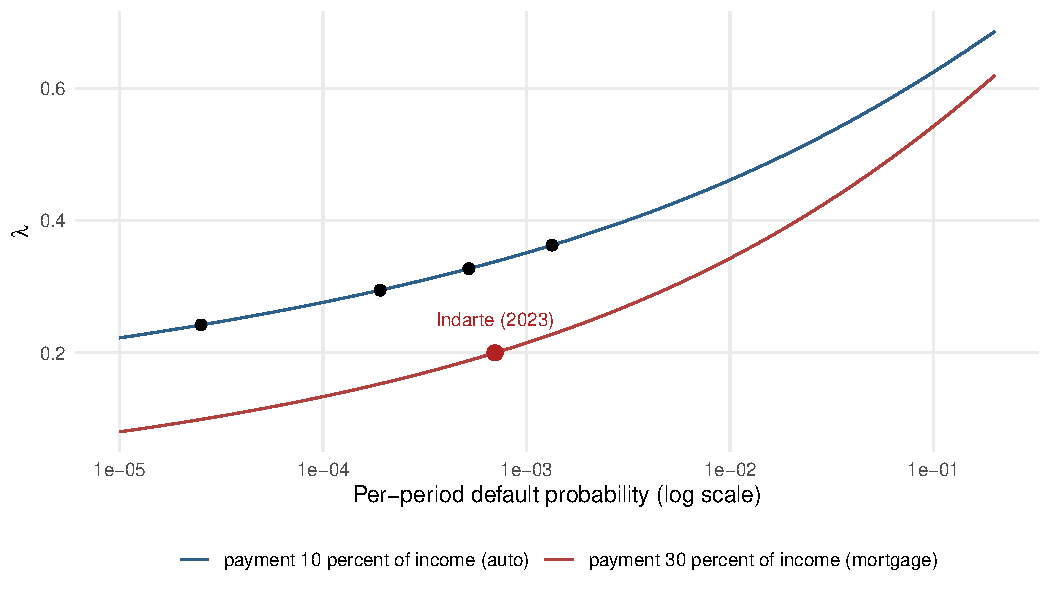
\includegraphics[width=0.75\textwidth]{figures/fig_lambda_curve.pdf}
\caption{The present-payment premium as a function of the per-period default probability, at two payment shares of income, calibrated through Indarte's (2023) value; the black points are the auto population and its score terciles.}
\label{fig:lambda_curve}
% replication: Code/local/lambda_by_default_rate.R; results/lambda_curve.csv, results/lambda_by_default_rate.csv
\end{figure}

The weight on a payment $s$ months ahead in Proposition \ref{prop:sensT} includes the marginal-utility ratio $\lambda$ of equation \eqref{eq:twoperiod}: the average marginal utility of a repayer at $s$, conditional on standing at today's default margin, relative to the marginal utility of the marginal defaulter herself. This appendix records the three sources of information on $\lambda$ that the paper uses, in the order of their weight: a measurement from a pair of experiments, a calibration from the persistence of the distress state, and two bounds.

\subsection{Measurement}

\citet{indarte_moral_2023} identifies two responses of bankruptcy filing for the same population: to a dollar of payment relief within the year, at an adjustable-rate reset, and to a dollar of seizable home equity at the filing date, at an exemption kink. The first is a liquid dollar at the decision date; the second is an illiquid dollar at the same date. Their ratio is a ratio of marginal utilities and not of dates, and the model produces it as a function of $\lambda$ alone, at any discount rate (Figure \ref{fig:ledger_rho}, bottom panel). The observed ratio crosses the model's line at $\lambda \approx 0.2$. This is the level through which the profile of equation \eqref{eq:lambda_p} passes, and the experiments' sets move little with it: the Dobbie--Song sets end at $1.20$ and $2.84$ under the profile and at $0.99$ and $1.97$ under a constant $0.2$ (Table \ref{tab:experiments}).

\subsection{Why $\lambda$ differs from one, and what determines it}\label{appendix:measuredrho}

Two forces govern the gap between the two marginal utilities. \emph{Income persistence}: if the distress that puts a borrower at the margin persists, a repayer at $s$ is still relatively poor and the two marginal utilities are close; if it is transitory, repayers are drawn from the unconditional distribution and $\lambda$ falls well below one. \emph{Consumption insurance}: households smooth, so consumption dispersion is smaller than income dispersion. Annual persistence of the idiosyncratic component of labor income is estimated at $\rho \approx 0.99$ under restricted income profiles and $0.82$ under heterogeneous profiles \citep{guvenen_empirical_2009}, $0.91$ in PSID data \citep{floden_idiosyncratic_2001}, and $0.95$ in \citet{storesletten_cyclical_2004}; for insurance, \citet{blundell_consumption_2008} estimate that consumption loads with coefficient about $0.64$ on permanent income shocks.

The object $\lambda$ requires is more specific than the persistence of labor income in the population: it is the persistence of the state of a borrower at the default margin. The credit-bureau panel measures it. Every auto tradeline with a manner-of-payment rating of thirty days past due or worse and no charge-off at one archive snapshot is followed to the next snapshot (mean gap $4.2$ months). Across 26.6 million such transitions, $72.7$ percent remain delinquent, $6.8$ percent charge off, and $20.5$ percent return to current; among mortgages the shares are $75.9$, $0.3$ and $23.8$ percent. The per-gap persistence of the distress state is $0.80$, or $0.52$ annualized. Distress is persistent but far from absorbing: a borrower at the margin expects, with probability near one half within a year, to be in an ordinary state at which her marginal utility is lower. That is the premium $\lambda$ measures, and a persistence of one half is the range in which the two-period calibration below places $\lambda$ well below one.

\subsection{Calibration}

The calibration embeds both forces in the two-period model: $\log y_2 = \varrho \log y_1 + \varepsilon$ with $\varrho = \rho^{T}$ for a horizon $T$ of $3.2$ years, stationary innovation variance, and consumption $c(y) = y^{\phi}$ with required payments reducing consumption one-for-one. Thresholds and $\lambda$ are computed exactly by the same routines as the baseline model. Table \ref{tab:mucorrection} reports $\lambda$ for $\gamma = 2$ across the persistence grid; the replication file contains $\gamma \in \{1, 3\}$.

\begin{table}[H]
\centering
\caption{The marginal-utility ratio $\lambda$ in the two-period calibration ($\gamma = 2$)}
\label{tab:mucorrection}
\begin{tabular}{lccc}
\toprule
Annual persistence of the distress state & $\phi=1.00$ & $\phi=0.64$ & $\phi=0.40$ \\
\midrule
0.52 (measured, this appendix) & 0.45 & 0.33 & 0.24 \\
0.82 \citep{guvenen_empirical_2009} & 0.72 & 0.64 & 0.51 \\
0.91 \citep{floden_idiosyncratic_2001} & 0.92 & 0.84 & 0.72 \\
0.95 \citep{storesletten_cyclical_2004} & 1.04 & 0.95 & 0.84 \\
0.99 \citep{guvenen_empirical_2009} & 1.09 & 1.00 & 0.97 \\
\bottomrule
\end{tabular}


\vspace{0.5em}
\noindent \small \textit{Notes:} $\lambda$ computed exactly in the two-period model with persistent income ($\varrho = \rho^{3.2}$) and consumption function $c(y)=y^{\phi}$; $\phi = 1$ is hand-to-mouth, $\phi = 0.64$ the permanent-shock pass-through of \citet{blundell_consumption_2008}, $\phi = 0.40$ a more fully insured benchmark. The first row evaluates the grid at the persistence of the distress state measured in the panel.
% replication: Code/local/mucorrection_calibration.R (results/mucorrection_table.csv), Code/exhibits/make_mucorrection_table.R
\end{table}

At the persistence measured in the panel the calibration gives $\lambda$ between $0.24$ and $0.45$, above the value of $0.20$ estimated from Indarte's pair. The higher persistence values of the labor-income literature give $\lambda$ near one; they describe the population's income process rather than the distress state's, and Table \ref{tab:mucorrection} reports the calibrated value across the whole band.

\subsection{Bounds}

One restriction bounds $\lambda$ without a preferred value, and one observation is consistent with every value in the band. \emph{Internal consistency}: the weight $\lambda D(s) Q(s)$ on a future payment cannot exceed one, so $\lambda \le 1$; and the run-off of Section \ref{sec:mainresults} requires that the remaining payments have positive weight, which is $\lambda > 0$. \emph{Borrowing rates}: a household whose weight on any later dollar against the dollar due now is $\lambda$ borrows at any rate below the implied premium, so the rates at which households borrow, a median card rate of 18 percent among revolvers in the Survey of Consumer Finances (Appendix \ref{appendix:beliefs}), are consistent with any $\lambda$ in the band and do not restrict it.

Because a common $\lambda$ rescales the weights on all future payments identically, the cross-sectional comparisons of Section \ref{sec:heterogeneity} do not depend on it; the first-order estimate from the run-off moves with $\lambda$ (Appendix \ref{appendix:formula}), which is one more reason the run-off is mapped through the model. Table \ref{tab:ladder} gives the correction ladder for the constant-weight estimate of the two margins, for comparison with the earlier literature.

\begin{table}[H]
\centering
\caption{The correction ladder for the constant-weight estimate, applied cumulatively}
\label{tab:ladder}
\begin{tabular}{lcccc}
\toprule
 & face value & + timing dispersion & + persistence & + default option \\
$\phi$ & & (Jensen, $\sigma_\Delta = 1.61$) &
(measured $\varrho = 0.517$) & ($h = 5.7\%$/yr) \\
\midrule
0.5 & 27.1\% & 30.1\% & 8.7\% & 2.5\% \\
0.7 & 27.1\% & 30.1\% & 18.3\% & 11.6\% \\
0.9 & 27.1\% & 30.1\% & 26.4\% & 19.3\% \\
\bottomrule
\end{tabular}

\vspace{0.5em}
\noindent \small \textit{Notes:} Corrections applied left to right, cumulatively, at three values of the consumption-insurance pass-through $\phi$, to the constant-weight ratio of the two margins.
% replication: Code/level/L5_ladder.R
\end{table}

\section{Proofs}
\label{appendix:proofs}

This appendix provides a complete derivation of the comparative statics in equation \eqref{eq:sensitivities}.

\subsection{Setup and Default Threshold}

The borrower defaults in period 1 by comparing:
\[
V_1^P(y_1) = u(y_1 - m) +
\delta \left[
\int_{y_2^*}^\infty u(y_2 - (L-m)) dF(y_2 \mid y_1)
+
\int_0^{y_2^*} (u(y_2) - \sigma) dF(y_2 \mid y_1)
\right]
\]
and
\[
V_1^N(y_1) = u(y_1) + \delta (u(y_2) - \sigma).
\]

The threshold $y_1^*$ satisfies $V_1^P(y_1^*) = V_1^N(y_1^*)$, and $p_1 = F(y_1^*)$, so:
\begin{equation}
\frac{\partial p_1}{\partial x} = f(y_1^*) \frac{\partial y_1^*}{\partial x},
\qquad x \in \{L,m\}.
\label{eq:pchain}
\end{equation}

\subsection{Differentiating the Threshold Condition}

Defining $\Delta(y_1;L,m) \equiv V_1^P(y_1) - V_1^N(y_1) = 0$ at $y_1 = y_1^*$, implicit differentiation gives:
\[
\frac{\partial y_1^*}{\partial x}
=
- \frac{\partial \Delta / \partial x}{\partial \Delta / \partial y_1}.
\]

\subsection{Derivative with Respect to $y_1$}
\[
\frac{\partial}{\partial y_1} \Delta(y_1;L,m)
=
u'(y_1 - m) - u'(y_1)
\equiv u'(C_1^P) - u'(C_1^N) < 0.
\]

\subsection{Derivative with Respect to $L$}

Only the continuation value depends on $L$:
\[
\frac{\partial \Delta}{\partial L}
=
-\delta (1-p_2)
E\!\left[ u'(C_2^P(y_2)) \,\middle|\, y_2 > y_2^* \right].
\]

Combining:
\[
\boxed{
\frac{\partial p_1}{\partial L}
=
f(y_1^*) \delta (1-p_2)\,
\frac{E[u'(C_2^P(y_2)) \mid y_2>y_2^*]}
{u'(C_1^{P*}) - u'(C_1^{N*})}.
}
\]

\subsection{Derivative with Respect to $m$}

The payment $m$ affects both current consumption and the future balance:
\[
\frac{\partial \Delta}{\partial m}
=
- u'(C_1^P)
- \frac{\partial \Delta}{\partial L}.
\]

Therefore:
\[
\boxed{
\frac{\partial p_1}{\partial m}
=
f(y_1^*)\frac{u'(C_1^P)}{u'(C_1^{P*}) - u'(C_1^{N*})}
-
\frac{\partial p_1}{\partial L}.
}
\]

\subsection{Discussion}

Increasing $L$ worsens future consumption while holding current consumption fixed; increasing $m$ worsens current consumption while reducing future obligations. The ratio of these channels maps cleanly to $\delta$.

% appendix_formula.tex: The formula with beliefs fixed, and its anchoring (2026-09-04).
\section{The Ratio Formula with Beliefs Fixed, and Its Anchoring}\label{appendix:formula}

This appendix derives the first-order estimates from the credit-bureau margins, the ratio formula with beliefs fixed, the anchoring of the term margin on the experiments, and the first-order run-off formula, reports what each returns on the data, and states why each is not the mapping the paper uses, a reason established in Appendix \ref{appendix:mcliquidity} or in Section \ref{sec:termmargin}. The estimates are reported so that the model-based estimates can be compared with them.

\subsection{The formula}
With an annuity contract, $m_s = m$ for $s \le T$, Proposition \ref{prop:sensT} writes each elasticity of the default probability as a weighted sum over the payment path. At decision month $s$ the borrower weighs the current payment, priced at the default threshold, against the remaining payments, priced at the repayers' marginal utility, $\lambda$ times the threshold value, discounted by $D(\cdot)$ and by survival in the loan $Q(\cdot)$:
\begin{equation}
W_s \;=\; 1 + \lambda \sum_{j=s+1}^{T} D(j-s)\,Q(j-s).
\label{eq:Ws}
\end{equation}
A penalty proportional to the remaining balance, $\kappa_B B_s$ with $B_s = m\,a(T-s; r)$ and $a(n; r) = (1-(1+r)^{-n})/r$ the annuity factor at the note rate $r$, adds a second channel to each elasticity. Writing $k = \kappa_B/\kappa$ for the ratio of the penalty scale to the payment scale, the ratio of the two elasticities at decision month $s$ is
\begin{equation}
R_s(\rho, k) \;=\; \frac{T\,\lambda\,D(T-s)\,Q(T-s) \;-\; k\,T\,(1+r)^{-(T-s)}}{W_s \;-\; k\,a(T-s; r)},
\label{eq:Rs}
\end{equation}
because the marginal payment added by a longer term falls at the end of the contract, and the remaining balance rises with the term at the rate $T(1+r)^{-(T-s)}/a(T-s;r)$; at $k = 0$ and $s = 1$, \eqref{eq:Rs} is the date-1 case of equation \eqref{eq:window} of the main text. The ratio for default within $K$ months aggregates decision months with the default-timing weights $\omega_s$, the hazard at $s$ times survival to $s$, normalized over $s \le K$:
\begin{equation}
R(K) \;\equiv\; \frac{\varepsilon_T(K)}{\varepsilon_m(K)} \;=\; \sum_{s \le K} \omega_s\, R_s(\rho, k).
\label{eq:RK}
\end{equation}
The penalty scale is reported as its share of the payment channel at the first decision month, $\phi = k\,a(T-1;r)/W_1 \in [0, 1)$, which makes the parameter space the same for every contract length and exit hazard. The inputs and their sources are: $\lambda = 0.2$ as a constant, the level the pair of experiments in Section \ref{sec:quasi} identifies, with a band from $0.1$ to $0.35$ (the anchored fit predates the profile of equation \eqref{eq:lambda_p} and is recorded as run); $Q(n) = e^{-h n/12}$ with $h$ the group's own exit hazard from payoff before maturity, corrected for exposure; $r = 0.08$ with a band from $0.05$ to $0.12$; $T$ the group's mean contract length; $\omega_s$ from the group's own default timing; and $D(n) = e^{-\rho n/12}$, the object of the fit. The asymmetry between the current payment and the later ones in \eqref{eq:Ws} is what the closed form $x/(e^x-1)$ omits; on the model's own simulations that omission overstates the ratio by a factor between 2.5 and 3 (Appendix \ref{appendix:mcliquidity}), and it is inside the formula here.

\subsection{What the profile identifies on its own}
Both channels in \eqref{eq:Rs} rise with the window: the preference channel because the marginal payment draws nearer at the rate $\rho + h$, the penalty channel because the balance amortizes in the denominator. Across the windows available, six to forty-eight months, a higher $\rho$ with a lower $\phi$ traces nearly the same curve as a lower $\rho$ with a higher $\phi$; the root mean squared distance between the best-matching curves at $\rho = 0$ and $\rho = 0.3$ is $0.04$, below the precision of any group. Fitted to the within-borrower profile, the bridged population profile, and every group profile, the formula reproduces each ($\chi^2$ below one on two degrees of freedom) while the confidence set for $\rho$ spans the whole grid. Contract-length bins do not resolve it: with an exit hazard near $0.22$ per year the weight on the marginal payment falls with the term through $Q$ rather than through $D$, so the gradient of $R$ in $T$ is nearly the same at every $\rho$. The profile therefore identifies the difference between the two channels: given $\rho$ it gives the penalty share, and given the penalty share it gives $\rho$.

\subsection{The anchoring}
Two measured objects supply what the profile lacks. The first moves the penalty channel and nothing else. Loans below a state's deficiency threshold cannot be pursued for the balance after repossession, so their default cost scales less with the remaining balance while their payment stream is unchanged; the difference in the ratio between these loans and loans of the same size in other states, $\Delta R(K) = R_{\text{no pursuit}}(K) - R_{\text{pursuit}}(K)$, is a function of $(\phi_{\text{pursuit}}, \phi_{\text{no pursuit}})$ at any $\rho$ (Section \ref{sec:termmargin}). The second anchors $\rho$: the rescheduling-against-write-down pair in Section \ref{sec:quasi}, read at a single decision date as the anchoring was run, fits best at $\rho^\ast = 0$ and accepts rates below $0.03$ at the five percent level and below $0.08$ at one percent over a four-year horizon for a distressed population; aggregated over the pair's own outcome window the set extends to $1.2$, which is why the paper no longer uses the pair as an anchor.

In the anchor group, the pooled sample or the bottom score tercile, the population closest to that experiment's, $\rho$ is set to $\rho^\ast$ and $(\phi_A, \phi_{\text{np},A})$ are fitted to the profile and the contrast. Their difference is the deficiency component of the balance channel, and $\psi = \phi_A/(\phi_A - \phi_{\text{np},A})$ is the ratio of the whole balance channel, whatever scales with the balance, to its deficiency part. In every other group $\psi$ is imposed, $\phi_{\text{np},g} = \phi_g(1 - 1/\psi)$, and $(\rho_g, \phi_g)$ are fitted to the group's own profile and contrast with the group's own exit hazard, timing weights and contract length. An alternative anchoring imposes the no-pursuit share itself, $\phi_{\text{np},g} = \phi_{\text{np},A}$; agreement between the two is reported as the check on the assumption. Groups too thin for a contrast inherit $\phi$ from their parent score tercile and fit $\rho$ alone. Uncertainty combines the profile confidence set given the anchoring with the band over $\rho^\ast$ from zero to the date-1 one percent bound of $0.08$ and over $\lambda \in \{0.1, 0.2, 0.35\}$.

The construction was to rest on three facts and one assumption. The discount rate of the anchor is identified by a rule-based experiment on a population the anchor group resembles. The payment margin, the object the experiments manipulate, is a stable parameter in the bureau data and is reproduced across the population by the specification of Appendix \ref{appendix:bridge}. The recourse contrast is the one bureau moment that moves a single channel. The assumption is that the balance channel scales with its deficiency component; it is imposed in two ways, and rankings of groups that survive both do not depend on it. What the construction does not provide is point identification of a discount rate for each group from the bureau alone: the population-scale statement is a discount rate across people and time given the population-level anchor.

\subsection{Recovery on simulated data, and the failure of the term-margin anchoring}
Two checks were run. On profiles generated from \eqref{eq:RK} with known parameters by group and noise at the precision of the sample, the anchored fit recovers the ordering of $\rho$ across groups and covers the true value in five of six groups. On the model of Appendix \ref{appendix:mcliquidity} itself, with the balance penalty at its full value for pursued loans and at forty percent of it for loans that cannot be pursued, the anchored fit was applied to seven simulated groups with known $(\rho, \sigma)$: it recovers the groups that share the anchor's penalty level ($0.30 \to 0.41$, $0.17 \to 0.19$, $0.03 \to 0.00$) and fails for the groups at twice the penalty ($0.08 \to 1.85$, $0.17 \to 1.60$, $0.30 \to 1.80$), with the anchor's own fit rejected ($\chi^2$ of 575 on twelve moments). The first-order formula is not a faithful reduced form of the model's window profile. On the covariate-matched extract, moreover, the recourse contrast has 303 no-pursuit defaults and no power by group, and the population profile exceeds one above the fifth score decile, which the preference channel cannot produce at any $\rho$. The term margin is therefore not used to identify a discount rate; its profile is reported as a finding in Section \ref{sec:termmargin}, and the designs applied to it are listed in Appendix \ref{appendix:strategies}.

\subsection{The payment margin over the life of the loan}\label{appendix:runoff}
Under the first-order formula $\rho$ would be identified from the payment margin itself, over the life of the loan. At loan age $s$ the incentive to default is $m W_s - \theta C_s$, with $W_s$ from \eqref{eq:Ws} evaluated over the $T - s$ remaining payments and $C_s$ the penalty base, measured by the charged-off amount. Under a logistic latent with a scale that does not change with loan age, the elasticity of the default hazard at age $s$ to $\log m$ is proportional to $W_s - \theta (C_s/m)\,\varepsilon_m$, where $\varepsilon_m = 1.04$ is the measured elasticity of the charged-off amount to the payment. $W_s$ runs off as the contract shortens, at a rate set by $\rho + h$ and scaled by $\lambda$; the penalty base runs off with the balance. Under that formula the shape of the run-off, not its level, would identify $\rho$: when the far payments have little weight, $W_s$ stays flat until the last two years and then drops, and when they have much, it declines from the start. Remark \ref{rem:option} and Appendix \ref{appendix:mcliquidity} establish that the stopping problem calibrated to the sample's default rate, with i.i.d.\ or with persistent income, produces the same shape at every rate, at a payment elasticity ten times the data's (Appendix \ref{appendix:persistent}).

The run-off is measured on the auto panel by a linear probability model of default within each loan-age bin (0--6, 6--12, 12--18, 18--24, 24--36, 36--48, 48--60 months), among loans that survived to the bin, on $\log m$ and $\log T$ with the fixed effects of Appendix \ref{appendix:bridge}, by group; the elasticity is the coefficient over the bin's hazard. The fit is
\begin{equation}
\varepsilon_m(s) \;=\; A\,\big[\,W_s(\rho, \lambda, h) - \theta\,(C_s/m)\,\varepsilon_m\,\big],
\label{eq:runoff}
\end{equation}
by weighted least squares on a $(\rho, \theta)$ grid with the scale $A$ in closed form, $\lambda = 0.2$, $h$ the group's own exit hazard, $T$ its mean contract length and $C_s/m$ from the charged-off share by loan age scaled to the group's level. The confidence set for $\rho$ is the $\chi^2(1)$ cut of the profile. Figure \ref{fig:runoff_profiles} in the main text shows the measured run-off for the pooled sample, the two score terciles and three income quartiles against the model's range: flat for three years and then falling, with the same shape in every group.



\subsection{Results}
The measured run-off and the model's reproduction of it are reported in Sections \ref{sec:mainresults} and \ref{sec:heterogeneity}. Fitted with the first-order formula \eqref{eq:runoff} at $\lambda = 0.2$ and the panel's exit hazard, the pooled profile on 61- to 72-month contracts returns an annual rate of $0.56$ with a set from $0.40$ to $0.84$, and the group profiles return rates from $0.1$ to $1.3$; these numbers are not rates, because Appendix \ref{appendix:mcliquidity} shows the formula returns rates near $3$ on the model's own simulations at true rates of $0.03$ to $0.10$. The paper matches the profile to the model's own run-off, and every group's set spans the grid.

Three caveats accompany the result. The proportionality of the elasticity to the incentive rests on a latent scale that does not change with loan age. First-payment defaults, which do not respond to the payment, lower the first bin and cost fit in the pooled sample ($\chi^2$ of 8.8 on four degrees of freedom). The exit hazard computed from monthly sightings is a lower bound, and the outcome is charge-off; the monthly one-percent panel with closure dates and first 90-day delinquency is the check on both.


% appendix_ladder.tex: the across-borrower term margin adjusted for the penalty and selection, as the check on the within-borrower
% estimate (Code/local/bureau_rho_ladder.R, window_formula.R; exhibits make_ladder_tables.R), the term margin across and
% within borrower by decile (I6f), and the ladder by group. Moved from the main text on 2026-09-16.
\section{The Across-Borrower Term Margin, Adjusted}\label{appendix:ladder}

The bureau's contracts supply both responses the sufficient statistic of Proposition \ref{prop:sensT} needs: a longer contract at the same monthly payment adds payments at the end, and the payment margin moves every payment at once. Their ratio across borrowers, estimated within lender, place and score-by-income cells on 7.6 million auto loans, contains the two channels Proposition \ref{prop:termmargin} names besides the far payments' weight, the balance-scaled penalty and selection into contract length, and Section \ref{sec:termmargin} measures the first. The paper's estimate is the within-borrower one of Section \ref{sec:rate_people}, in which holding the borrower fixed removes selection by design and the penalty channel has decayed by twenty-four months. This appendix is the check: it starts from the across-borrower ratio at twelve months, adjusts for the measured size of each channel one at a time, and reports the rate the window formula returns from the adjusted ratio, with the within-borrower estimate as the reference. The procedure is the one the sufficient-statistics literature follows when a formula derived from a model is evaluated with the best available estimates of its inputs and the identification of each input is stated: \citet{davila_exemptions_2020} derives the optimal bankruptcy exemption as a function of four measurable objects, estimates the sensitivity of credit supply to exemptions from a branch fixed-effects regression on state exemption changes, and reports the sensitivity of the conclusion to the assumed utility parameters.

\subsection{The adjustments}

The outcome is default within twelve months of origination, which removes the exposure term because every loan is observed over the same window. The raw ratio $R_0 = \varepsilon_T/\varepsilon_m$ is $0.01$ for charge-off and $-0.77$ for 90-day delinquency: at face value the far payments have no weight, and the formula returns a rate of one or above. The first adjustment is the penalty channel. A longer contract at the same payment is a larger balance, and default forfeits more of it, which lowers default and biases the term response downward. The deficiency-judgment contrast of Section \ref{sec:termmargin} (Table \ref{tab:term_deficiency}) measures the deficiency part of that channel: where the lender cannot pursue the balance, the term elasticity is higher by $0.36$ (standard error $0.13$) at twelve months. The whole balance channel is $\psi$ times its deficiency part; $\psi = 1$ is the case in which the deficiency judgment is the whole of the balance-scaled cost, and $\psi = 2.5$ allows the credit record's report of the charge-off to add one and a half times as much again, and both are reported because the data do not measure $\psi$. The second adjustment is selection into contract length. Lenders screen with maturity and borrowers sort into it \citep{hertzberg_screening_2018}, so the across-borrower term response differs from the within-borrower one; the within-borrower estimate on multi-loan borrowers is $0.19$ below the same-sample across-borrower estimate at twelve months (Table \ref{tab:within_by_group}), and that difference is applied. The adjusted ratio is mapped to a rate by the window formula of equation \eqref{eq:window} at $K = 12$ with the panel's default timing, $T$ the mean contract length, $h$ the panel's exit hazard and the marginal-utility profile of equation \eqref{eq:lambda_p} at the population's default rate ($\lambda_{60} = 0.34$ for the auto population). The exit hazard here is the panel's gross payoff hazard, $0.22$ per year, whereas the within-borrower estimate of Section \ref{sec:rate_people} uses the hazard net of servicer transfers, $0.19$; with these inputs the formula's value at a rate of zero is $0.43$, and with the within-borrower estimate's it is $0.59$.

Table \ref{tab:bureau_ladder} reports the pooled result. For charge-off with $\psi = 1$, the penalty adjustment alone takes the ratio to $0.81$, above the formula's value at a rate of zero, and the selection adjustment brings it to $0.39$ (standard error $0.31$), which the formula maps to $\rho = 0.04$ with a set from zero to infinity; the set is wide because the two adjustments are measured once, on pooled samples, with standard errors of the order of the ratio itself. The premium's shape is a second-order input here: with a constant premium of $0.2$ at every later date the adjusted ratio maps to $0.15$ and with $0.5$ to $0.18$, inside the same set. With $\psi = 2.5$ the adjusted ratio is above the formula's ceiling and maps to zero with a set bounded at $0.32$. For 90-day delinquency the raw ratio is negative, and the adjustments do not bring it above zero at $\psi = 1$. What the procedure measures with precision is the size of the adjustments a rate taken from contracts across borrowers requires: the penalty channel and selection into contract length together move the term elasticity by more than half a payment elasticity, and the bureau's contracts have no variation that separates them from the far payments' weight. The adjusted across-borrower ratio, $0.04$ with a set that spans the grid, is consistent with the within-borrower estimate of $0.11$ and differs from it in precision: the adjustments cost the across-borrower object the precision that holding the borrower fixed keeps, and the agreement is the check that the penalty channel the within-borrower estimate leaves unsubtracted at twenty-four months is of the size subtracted here at twelve.

\subsection{Selection measured by group}

The selection adjustment above is one number. Table \ref{tab:within_by_group} measures it decile by decile, on the 13.5 million borrowers with two or more auto loans in the ten-percent archive, 65 million loans, within borrower and origination-year cells, by comparing the term elasticity across borrowers within lender-year cells with the same elasticity within borrower, the group being fixed by the borrower's score at first sight so that both loans of a borrower fall in one decile. Across borrowers the term elasticity at twenty-four months climbs from $-0.39$ in the bottom decile to $1.21$ in the top. Within borrower it rises from $0.19$ to $0.43$, and the within-borrower payment elasticity rises with it, from $0.36$ to $0.87$, so the ratio of the two, the object of Proposition \ref{prop:sensT}, is between $0.32$ and $0.53$ in every decile with standard errors of $0.02$ to $0.10$. The across-borrower gradient is selection into contract length, from $+0.58$ in the bottom decile to $-0.78$ in the top, and it has the sign structure of \citet{hertzberg_screening_2018}: positive for subprime borrowers, whom lenders screen with maturity, and negative for prime borrowers, who choose long terms themselves. At twelve months the within-borrower ratio has a gradient, from $-1.58$ in the bottom decile to about $0.3$ in the top three, so the far payments' weight measured within the first year is negative for the borrowers whose balances are charged off most, which is the balance-scaled penalty of Proposition \ref{prop:termmargin}, and the twenty-four-month ratio is where the penalty and the preference channel are both in view. By income quartile, on the 1.35 million multi-loan borrowers with an income at first sight, the twenty-four-month ratio is $0.34$, $0.52$, $0.45$ and $0.27$ from the bottom quartile to the top, with standard errors of $0.05$ to $0.12$, and selection runs from $+0.38$ to $-0.81$: no monotone gradient in income, as in score. The rise of the within-borrower ratio from twelve to twenty-four months, from $-0.70$ to $0.55$ in the pooled sample, each measured to a few hundredths, is a fact about the timing of the far payments' weight that the model of Appendix \ref{appendix:multiperiod} does not reproduce at any rate or penalty (Appendix \ref{appendix:mcliquidity}); it is reported as measured.

\begin{table}[H]
\centering
\caption{The term margin across and within borrower, by score decile}
\label{tab:within_by_group}
\small
\resizebox{\textwidth}{!}{\begin{tabular}{lrrrrrrrrr}
\toprule
 & & \multicolumn{4}{c}{Within twelve months} & \multicolumn{4}{c}{Within twenty-four months} \\
\cmidrule(lr){3-6}\cmidrule(lr){7-10}
Score decile & Loans & Across & Within & Selection & Ratio & Across & Within & Selection & Ratio \\
\midrule
All & 62,518,904 & -0.12 (0.01) & -0.31 (0.01) & -0.19 (0.01) & -0.70 (0.02) & 0.22 (0.00) & 0.30 (0.01) & 0.08 (0.01) & 0.55 (0.01) \\
1 & 6,200,400 & -0.68 (0.01) & -0.45 (0.01) & 0.22 (0.02) & -1.58 (0.07) & -0.39 (0.01) & 0.19 (0.01) & 0.58 (0.01) & 0.53 (0.03) \\
2 & 6,212,641 & -0.54 (0.02) & -0.35 (0.02) & 0.19 (0.02) & -0.95 (0.05) & -0.29 (0.01) & 0.23 (0.01) & 0.52 (0.01) & 0.50 (0.02) \\
3 & 6,223,474 & -0.38 (0.02) & -0.22 (0.02) & 0.16 (0.03) & -0.44 (0.04) & -0.16 (0.01) & 0.27 (0.01) & 0.43 (0.02) & 0.47 (0.02) \\
4 & 6,224,917 & -0.22 (0.02) & -0.13 (0.03) & 0.09 (0.03) & -0.23 (0.04) & 0.02 (0.01) & 0.29 (0.02) & 0.27 (0.02) & 0.44 (0.02) \\
5 & 6,221,828 & -0.08 (0.02) & -0.08 (0.03) & -0.00 (0.04) & -0.13 (0.04) & 0.16 (0.02) & 0.27 (0.02) & 0.11 (0.02) & 0.37 (0.03) \\
6 & 6,239,127 & 0.27 (0.03) & 0.04 (0.04) & -0.23 (0.05) & 0.04 (0.05) & 0.45 (0.02) & 0.27 (0.02) & -0.19 (0.03) & 0.32 (0.03) \\
7 & 6,260,275 & 0.56 (0.04) & 0.05 (0.05) & -0.51 (0.07) & 0.05 (0.06) & 0.78 (0.03) & 0.35 (0.03) & -0.43 (0.04) & 0.39 (0.04) \\
8 & 6,285,765 & 0.96 (0.06) & 0.33 (0.07) & -0.63 (0.09) & 0.31 (0.07) & 1.05 (0.04) & 0.40 (0.04) & -0.65 (0.06) & 0.40 (0.04) \\
9 & 6,315,195 & 1.09 (0.07) & 0.39 (0.09) & -0.70 (0.11) & 0.41 (0.10) & 1.21 (0.05) & 0.41 (0.05) & -0.81 (0.07) & 0.44 (0.06) \\
10 & 6,335,282 & 1.23 (0.09) & 0.32 (0.12) & -0.92 (0.15) & 0.32 (0.12) & 1.21 (0.06) & 0.43 (0.08) & -0.78 (0.10) & 0.49 (0.10) \\
\midrule
\multicolumn{10}{l}{\emph{Income quartile (borrowers with income at first sight)}} \\
1 & 1,541,188 & -0.49 (0.03) & -0.43 (0.03) & 0.06 (0.05) & -1.07 (0.10) & -0.21 (0.02) & 0.17 (0.02) & 0.38 (0.03) & 0.34 (0.05) \\
2 & 1,557,805 & -0.30 (0.04) & -0.27 (0.05) & 0.03 (0.06) & -0.52 (0.10) & -0.02 (0.03) & 0.31 (0.03) & 0.32 (0.04) & 0.52 (0.05) \\
3 & 1,572,950 & 0.45 (0.06) & 0.06 (0.08) & -0.39 (0.10) & 0.08 (0.11) & 0.61 (0.04) & 0.36 (0.05) & -0.25 (0.07) & 0.45 (0.07) \\
4 & 1,578,545 & 0.86 (0.12) & -0.09 (0.16) & -0.96 (0.20) & -0.17 (0.29) & 1.03 (0.08) & 0.22 (0.09) & -0.81 (0.12) & 0.27 (0.12) \\
\bottomrule
\end{tabular}
}
\vspace{0.5em}
\begin{minipage}{0.92\textwidth}
\noindent \small \textit{Notes:} Elasticities of default within twelve and twenty-four months to the contract length at the same payment (with the log payment as the second regressor), on borrowers with two or more auto loans in the ten-percent archive with a credit score at first sight, by the decile of that score. Across: lender-year fixed effects on the same sample; within: borrower and origination-year fixed effects; selection: within minus across, with the standard error of the difference; ratio: the within-borrower term elasticity over the within-borrower payment elasticity, delta-method standard error. Standard errors clustered by borrower.
\end{minipage}
% replication: Code/identification/I6f_within_person_by_group.R, Code/exhibits/make_within_group_table.R
\end{table}

\begin{table}[H]
\centering
\caption{The across-borrower term margin adjusted for the penalty and selection, pooled}
\label{tab:bureau_ladder}
\small
\resizebox{\textwidth}{!}{\begin{tabular}{llrrrrrr}
\toprule
Outcome & $\psi$ & $\varepsilon_m$ & $\varepsilon_T$ & Raw $R$ ($\rho$) & + penalty ($\rho$) & + selection $R$ (s.e.) & $\rho$ [95\% set] \\
\midrule
Charge-off within twelve months & 1.0 & 0.45 (0.02) & 0.01 (0.05) & 0.01 (1.06) & 0.81 (0.00) & 0.39 (0.31) & 0.04 [0.00, $\infty$] \\
Charge-off within twelve months & 2.5 & 0.45 (0.02) & 0.01 (0.05) & 0.01 (1.06) & 2.01 (0.00) & 1.59 (0.73) & 0.00 [0.00, 0.32] \\
90-day delinquency within twelve months & 1.0 & 0.35 (0.02) & -0.27 (0.04) & -0.77 ($\infty$) & 0.25 (0.19) & -0.29 (0.39) & $\infty$ [0.00, $\infty$] \\
90-day delinquency within twelve months & 2.5 & 0.35 (0.02) & -0.27 (0.04) & -0.77 ($\infty$) & 1.78 (0.00) & 1.24 (0.92) & 0.00 [0.00, $\infty$] \\
\midrule
Rule-based experiments, Dobbie--Song pair (for reference) & & & & & & & best fit 0.00; [0.00, 1.20] (5\%), [0.00, 2.84] (1\%) \\
\bottomrule
\end{tabular}
}
\vspace{0.5em}
\begin{minipage}{0.92\textwidth}
\noindent \small \textit{Notes:} Auto loans in the monthly one-percent panel (7.6 million); elasticities of default within twelve months to the payment ($\varepsilon_m$) and to the contract length at the same payment ($\varepsilon_T$), with the cells of Table \ref{tab:main_margins} (lender by origination year, zip3 by origination year, score ventile by income quartile). Raw $R = \varepsilon_T/\varepsilon_m$; the penalty adjustment adds $\psi \times 0.36$ to $\varepsilon_T$ (the deficiency-judgment contrast at twelve months, small-loan specification, ten-percent extract); the selection adjustment adds $-0.19$ (within-borrower minus across-borrower term elasticity at twelve months on the multi-loan borrowers of the ten-percent archive, Table \ref{tab:within_by_group}). The formula maps the adjusted ratio to $\rho$ with the profile of equation \eqref{eq:lambda_p} at the panel's default rate ($\lambda_{60} = 0.34$), the panel's gross payoff hazard $0.22$ (Table \ref{tab:rho_within} uses the hazard net of servicer transfers, $0.19$) and $T = 60$ months; ratios above the formula's value at $\rho = 0$ ($0.43$ at these inputs) map to zero, ratios at or below zero to infinity. Sets: the delta-method standard error of the adjusted ratio, including the deficiency contrast's, taken through the formula. The last row reports the Dobbie--Song pair for reference: its best fit and the sets it accepts at the five and one percent levels (Table \ref{tab:experiments}).
\end{minipage}
% replication: Code/local/bureau_rho_ladder.R, Code/local/window_formula.R, Code/exhibits/make_ladder_tables.R
\end{table}

\subsection{The adjusted ratio by group}\label{appendix:strategies:groupladder}

Table \ref{tab:bureau_rho_groups} applies the same adjustments to every group, with the group's own marginal-utility profile, exit hazard and contract length and the pooled adjustments scaled by the group's charged-off share of the balance. The adjusted ratios are the measured objects, and their ordering is the same at both penalty scalings: the bottom score tercile and the bottom income quartile have negative adjusted ratios, $-0.40$ ($0.29$) and $-0.40$ ($0.32$), which the formula maps to no weight on far payments, while the top two score terciles and the top two income quartiles have adjusted ratios at or above the formula's value at a rate of zero, $0.37$ to $0.43$ at those groups' inputs, which it maps to full weight. Applied group by group the procedure returns boundary values of the mapping, ratios measured to about $\pm 0.3$; the ordering across groups is the exposure of Section \ref{sec:heterogeneity} seen through the term margin, since the payment elasticity in the denominator rises with the score and with income, and it is not a gradient in the rate, which the within-borrower design of Section \ref{sec:rate_people} measures directly and finds flat.

\begin{table}[H]
\centering
\caption{The adjusted across-borrower ratio by group}
\label{tab:bureau_rho_groups}
\small
\resizebox{\textwidth}{!}{\begin{tabular}{llrrrrrrrr}
\toprule
Dimension & Group & Loans & $\lambda_T$ & $\varepsilon_m$ & $\varepsilon_T$ & Raw $R$ & Corrected $R$ (s.e.) & $\rho$ [set], $\psi = 1$ & $\rho$ [set], $\psi = 2.5$ \\
\midrule
All &  & 7,355,247 & 0.34 & 0.45 & 0.01 & 0.01 & 0.39 (0.31) & 0.04 [0.00, $\infty$] & 0.00 [0.00, 0.32] \\
Score tercile & 1 & 2,472,131 & 0.38 & 0.48 & -0.37 & -0.77 & -0.40 (0.29) & $\infty$ [0.36, $\infty$] & 0.00 [0.00, $\infty$] \\
Score tercile & 2 & 2,455,327 & 0.31 & 0.79 & 0.46 & 0.58 & 0.74 (0.18) & 0.00 [0.00, 0.00] & 0.00 [0.00, 0.00] \\
Score tercile & 3 & 2,427,789 & 0.26 & 0.47 & 1.31 & 2.81 & 2.95 (0.65) & 0.00 [0.00, 0.00] & 0.00 [0.00, 0.00] \\
Income quartile & 1 & 1,846,938 & 0.38 & 0.45 & -0.37 & -0.83 & -0.40 (0.32) & $\infty$ [0.27, $\infty$] & 0.00 [0.00, $\infty$] \\
Income quartile & 2 & 1,851,364 & 0.34 & 0.57 & 0.13 & 0.22 & 0.47 (0.23) & 0.00 [0.00, 1.06] & 0.00 [0.00, 0.13] \\
Income quartile & 3 & 1,845,440 & 0.30 & 0.82 & 0.58 & 0.71 & 0.83 (0.17) & 0.00 [0.00, 0.00] & 0.00 [0.00, 0.00] \\
Income quartile & 4 & 1,811,505 & 0.27 & 0.74 & 0.63 & 0.84 & 0.96 (0.25) & 0.00 [0.00, 0.00] & 0.00 [0.00, 0.00] \\
Region & MW & 1,598,359 & 0.34 & 0.50 & 0.04 & 0.07 & 0.44 (0.30) & 0.00 [0.00, $\infty$] & 0.00 [0.00, 0.26] \\
Region & NE & 1,160,318 & 0.33 & 0.67 & 0.28 & 0.42 & 0.63 (0.23) & 0.00 [0.00, 0.31] & 0.00 [0.00, 0.00] \\
Region & S & 2,962,049 & 0.35 & 0.39 & -0.10 & -0.25 & 0.18 (0.35) & 0.27 [0.00, $\infty$] & 0.00 [0.00, $\infty$] \\
Region & W & 1,581,037 & 0.34 & 0.49 & -0.06 & -0.13 & 0.23 (0.29) & 0.20 [0.00, $\infty$] & 0.00 [0.00, 1.11] \\
Cohort & 2005-09 & 1,995,599 & 0.31 & 0.54 & -0.35 & -0.65 & -0.45 (0.27) & $\infty$ [0.57, $\infty$] & 0.06 [0.00, $\infty$] \\
Cohort & 2010-12 & 1,226,517 & 0.33 & 0.38 & -0.21 & -0.55 & -0.27 (0.36) & $\infty$ [0.00, $\infty$] & 0.00 [0.00, $\infty$] \\
Cohort & 2013-15 & 1,077,245 & 0.35 & 0.41 & 0.01 & 0.02 & 0.41 (0.39) & 0.03 [0.00, $\infty$] & 0.00 [0.00, 0.67] \\
Cohort & 2016-18 & 1,108,633 & 0.35 & 0.44 & 0.13 & 0.29 & 0.68 (0.45) & 0.00 [0.00, $\infty$] & 0.00 [0.00, 0.14] \\
Cohort & 2019-21 & 1,045,442 & 0.35 & 0.38 & 0.04 & 0.12 & 0.67 (0.47) & 0.00 [0.00, $\infty$] & 0.00 [0.00, 0.17] \\
Cohort & 2022+ & 901,811 & 0.36 & 0.39 & 0.06 & 0.16 & 0.81 (0.48) & 0.00 [0.00, $\infty$] & 0.00 [0.00, 0.02] \\
\bottomrule
\end{tabular}
}
\vspace{0.5em}
\begin{minipage}{0.92\textwidth}
\noindent \small \textit{Notes:} Charge-off within twelve months; the adjustments of Table \ref{tab:bureau_ladder} with the group's own marginal-utility profile ($\lambda_T$ is its weight on the last payment; Appendix \ref{appendix:mucorrection}), exit hazard and mean contract length, and the pooled adjustments scaled by the group's charged-off share of the balance. Cohorts are origination years.
\end{minipage}
% replication: Code/local/bureau_rho_ladder.R, Code/exhibits/make_ladder_tables.R
\end{table}


% appendix_experiments.tex: the rule-based experiments: posterior summaries under a flat prior (moved from Section 3.4), the payment path of every treatment and the p-value curve of every pair.
\section{The Rule-Based Experiments: Posterior Summaries and Exhibits}\label{appendix:experiments}

This appendix reports, for the rule-based experiments of Section \ref{sec:quasi}, the posterior summaries of the rate under a flat prior, the payment path of every treatment arm, and the $p$-value curve of every pair together with the near-horizon responses across settings and Indarte's pair as the model produces it.

\subsection{The treatments and the model's estimate from each pair}

\begin{table}[H]
\centering
\caption{Rule-based experiments as payment-path treatments, and the model's estimate from each pair}
\label{tab:experiments}
\resizebox{\textwidth}{!}{\begin{tabular}{lllllll}
\toprule
\multicolumn{7}{l}{\textit{Panel A: treatments as payment-path changes}} \\
Study & Treatment & Type & Far payments at & Outcome & Effect, pp (s.e.) & Base, \% \\
\midrule
\citet{ganong_liquidity_2020} & Principal forgiveness, payments fixed 5 years & relief & 5--26 years & 90+ days delinquent at any point, modi & +1.20 (3.18) & 19.0 \\
\citet{ganong_liquidity_2020} & Deeper payment reduction, maturity to 40 years & rescheduling & 22--40 years & 90+ days delinquent within two years o & -0.38 (0.08) & 32.1 \\
\citet{indarte_moral_2023} & Seizable home equity at filing & value of default & at decision & Chapter 7/13 filing in the quarter & -0.019 (0.0024) & 0.7 \\
\citet{indarte_moral_2023} & ARM reset: lower payment for 12 months & relief & within 1 year & filing in each of the 12 months after  & -0.21 (0.06) & 0.7 \\
\citet{dobbie_targeted_2020} & Interest write-down: last 10 payments forgiven & relief & 3.5--4.3 years & bankruptcy filing within 5 years & -3.00 (0.90) & 10.5 \\
\citet{dobbie_targeted_2020} & Payment cut, 18 extra months, fees up & rescheduling & 4.3--5.8 years & bankruptcy filing within 5 years & +2.30 (1.10) & 10.5 \\
\citet{dobbie_targeted_2020} (median) & Write-down: last 4 payments forgiven & relief & 3.8--4.2 years & bankruptcy filing within 5 years & -0.99 (0.52) & 10.4 \\
\citet{dobbie_targeted_2020} (median) & Payment cut, 4 extra months & rescheduling & 4.2--4.5 years & bankruptcy filing within 5 years & +0.70 (0.42) & 10.4 \\
\citet{fiorin_moratorium_2026} & 3-month deferral, fee, 3 payments after maturity & rescheduling & 6--8 months & loan repaid in full & +0.30 (1.30) & 42.0 \\
\citet{fuster_payment_2017} & 5/1 IO ARM reset: rate $-$3 pp, payment halved & relief (single arm) & from reset on & first 60-day delinquency & -56.30\% (3.00) & 1.7 \\
\citet{keys_mortgage_2014} & Agency 5/1 vs 7/1 reset: $-$\$125, $-$\$164 per month & relief (single arm) & years 1--2 & 60+ day mortgage delinquency, two year & -1.80 (1.00) & 4.5 \\
\citet{agarwal_policy_2017} & HAMP modification: $-$25\% payment, 5 years & relief, then step-up & years 1--5 & foreclosure completed within one year  & -12.45 (0.39) & -- \\
\midrule
\multicolumn{7}{l}{\textit{Panel B: the test of each pair against the model (joint test on the two arms; grid of $\rho$ from 0 to 3 by 0.01; decisions aggregated over the outcome window; survival from the study's exit hazards)}} \\
Pair & $\rho$ best fit & $p$ at $\rho = 0.02$ & $p$ at the estimate & $p$ at 0.22 & $\rho$ consistent at 5\% & $\rho$ consistent at 1\% \\
\midrule
Dobbie--Song pair (max arms), $\lambda_s$ profile & 0.00 & 0.925 & 0.734 & 0.538 & [0.00, 1.20] & [0.00, 2.84] \\
\quad same, arms correlated 0.5 & 0.00 & 0.938 & 0.774 & 0.597 & [0.00, 1.24] & [0.00, 2.24] \\
\quad same, constant $\lambda = 0.2$ & 0.05 & 0.913 & 0.865 & 0.622 & [0.00, 0.99] & [0.00, 1.97] \\
Dobbie--Song pair (median arms), $\lambda_s$ profile & 0.00 & 0.628 & 0.575 & 0.517 & [0.00, 3.00] & [0.00, 3.00] \\
Ganong--Noel pair, $\lambda_s$ profile & 3.00 & 0.246 & 0.396 & 0.502 & [0.00, 3.00] & [0.00, 3.00] \\
\bottomrule
\end{tabular}}
\vspace{0.5em}
\begin{minipage}{0.95\textwidth}
\small \textit{Notes:} Panel A codes each treatment as the change in dollars owed by month relative to the study's control; effects are the studies' reported estimates on the outcome and horizon shown. Panel B tests each pair of arms from the same population on the grid of $\rho$ from 0 to 3 by 0.01: the joint $\chi^2(1)$ distance of the two reported effects from the model's line effect$_1 = r(\rho)\,$effect$_2$, with $r(\rho)$ the ratio of the arms' weighted payment changes under exponential discounting, aggregated over the decision months of each study's outcome window with the study's own event timing (equation \eqref{eq:window}), survival from the study's own exit hazards (the re-default or filing hazard scaled by the uncured share, plus the payoff hazard), and the marginal-utility profile of equation \eqref{eq:lambda_p} at the study population's baseline rate and payment share, through Indarte's $0.2$; the rows marked ``same'' repeat the test with the two arms' sampling errors correlated at 0.5 (their covariance is not reported and the main rows treat them as independent) and with a constant $\lambda = 0.2$. The reference rates are the 2 percent social discount rate, the paper's estimate, and the laboratory median of 0.22. Sets are the rates on the grid not rejected at the stated level, as unions of intervals where they are not connected. Indarte's pair identifies $\lambda$ and is not tested for $\rho$.
\end{minipage}
% replication: Code/local/experiments_ledger.R, Code/exhibits/make_experiments_table.py; external/experiments_paths.csv, external/experiments_estimates.csv, results/experiments_rho_summary.csv
\end{table}

\begin{figure}[H]
\centering
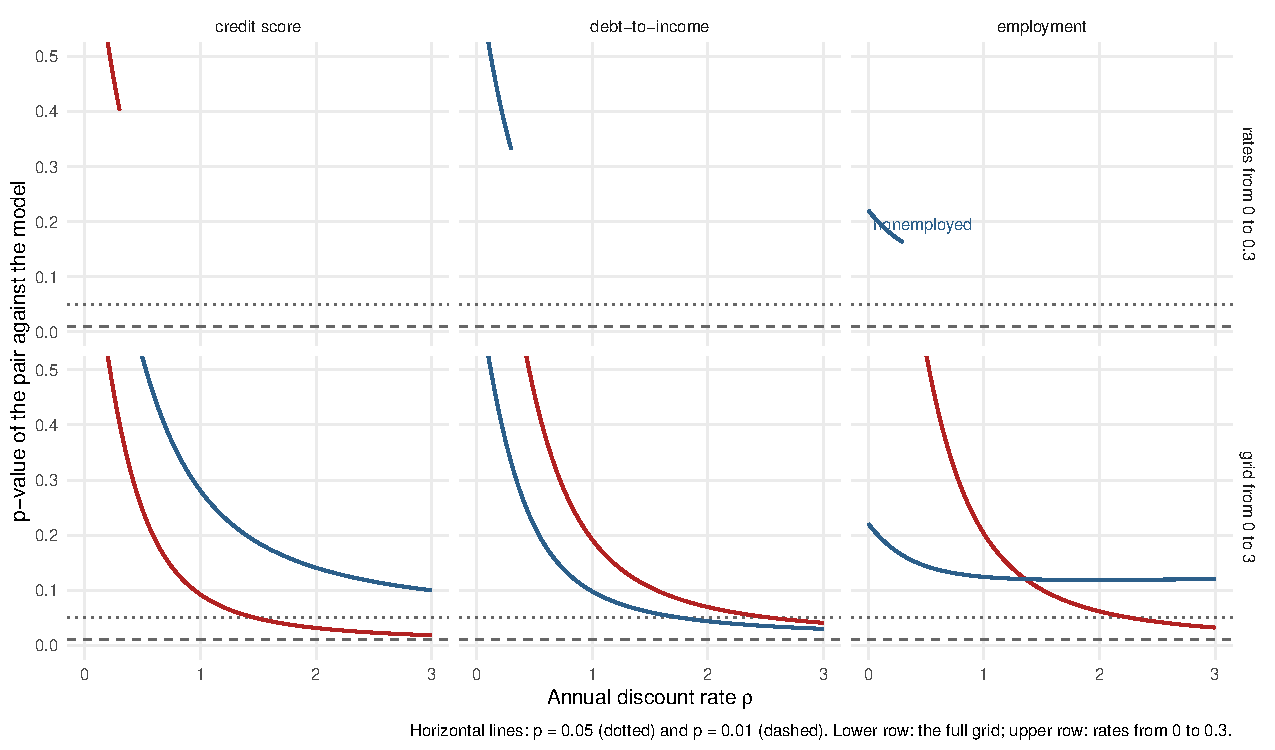
\includegraphics[width=\textwidth]{figures/fig_rho_subgroups.pdf}
\caption{The discount rate by subgroup in the Dobbie--Song experiment. Each curve is the $p$-value of the subgroup's pair of arms against the model's line on the grid of the annual rate from 0 to 3, aggregated over the five-year window at the marginal-utility profile, with survival from the study's exit hazards; the upper row repeats the lower on rates from 0 to 0.3; the dotted and dashed lines are five and one percent.}
\label{fig:rho_subgroups}
% replication: Code/local/experiments_rho_subgroups.R, Code/exhibits/make_rho_subgroups.R
\end{figure}

\begin{table}[H]
\centering
\caption{The discount rate by subgroup in the Dobbie--Song experiment}
\label{tab:rho_subgroups}
\small
\resizebox{\textwidth}{!}{\begin{tabular}{lrrrrrrll}
\toprule
Subgroup & write-down & payment reduction & $\rho$ best fit & $p$ at 0.02 & $p$ at the estimate & $p$ at 0.22 & $\rho$ consistent at 5\% & at 1\% \\
\midrule
All enrollees & $-0.030$ (0.009) & $+0.023$ (0.011) & 0.00 & 0.925 & 0.734 & 0.538 & [0.00, 1.20] & [0.00, 2.84] \\
Debt-to-income above median & $-0.035$ (0.012) & $+0.022$ (0.014) & 0.11 & 0.835 & 0.996 & 0.806 & [0.00, 2.54] & [0.00, 3.00] \\
Debt-to-income below median & $-0.023$ (0.011) & $+0.024$ (0.013) & 0.00 & 0.633 & 0.514 & 0.398 & [0.00, 1.76] & [0.00, 3.00] \\
Credit score above median & $-0.027$ (0.013) & $+0.018$ (0.014) & 0.07 & 0.924 & 0.947 & 0.800 & [0.00, 3.00] & [0.00, 3.00] \\
Credit score below median & $-0.032$ (0.011) & $+0.027$ (0.014) & 0.00 & 0.816 & 0.656 & 0.495 & [0.00, 1.47] & [0.00, 3.00] \\
Employed at baseline & $-0.035$ (0.010) & $+0.019$ (0.012) & 0.20 & 0.647 & 0.829 & 0.954 & [0.00, 2.26] & [0.00, 3.00] \\
Not employed at baseline & $-0.002$ (0.016) & $+0.028$ (0.018) & 0.00 & 0.215 & 0.194 & 0.174 & [0.00, 3.00] & [0.00, 3.00] \\
\bottomrule
\end{tabular}
}
\vspace{0.5em}
\begin{minipage}{0.95\textwidth}
\small \textit{Notes:} Effects on bankruptcy within five years of the maximum-intensity write-down and payment-reduction arms, by subgroup, from \citet{dobbie_targeted_2020}, Table 8 and Appendix Table A9 (standard errors in parentheses). The remaining columns test each pair against the model's line on the grid of the annual rate from 0 to 3 by 0.01, aggregated over the five-year window at the marginal-utility profile, with survival from the study's exit hazards and the two arms treated as independent, their covariance not being reported: the best-fitting rate, the $p$-value at the 2 percent social discount rate, at the paper's estimate and at the laboratory median of 0.22, and the sets of rates not rejected at the five and one percent levels. A set with two components has its second component in the region of high rates where the model predicts no write-down response. The pooled row uses the maximum-arm effects.
\end{minipage}
% replication: Code/local/experiments_rho_subgroups.R, Code/exhibits/make_rho_subgroups.R; results/experiments_rho_subgroups.csv
\end{table}

\subsection{Posterior summaries under a flat prior}

Turned into posterior weights under a flat prior, the estimates of Section \ref{sec:quasi} depend on the prior's support in a way that the $p$-value curve does not (Table \ref{tab:rho_posterior}). On the support $[0, 1]$ the Dobbie--Song posterior has its mode at zero, a mean of $0.36$, a 68 percent highest-density set of $[0, 0.47]$ and a 95 percent set of $[0, 0.88]$. On the support $[0, 3]$ the mode is again zero, but the mean is $0.66$ and a fifth of the posterior mass lies above $\rho = 1$, in the region where the write-down is predicted to do little: the mass is the prior's, not the experiment's, because a flat prior over a wide region of low likelihood accumulates weight that no point in the region earns. Pooling the pair with Ganong--Noel's under one rate changes little on either support, since the second pair's likelihood is nearly flat: the pooled mean is $0.40$ on $[0, 1]$ and $0.72$ on $[0, 3]$, with 68 percent sets of $[0, 0.51]$ and $[0, 0.80]$. The mean of a posterior is not the right summary of this evidence, and the paper does not report one as its rate; the experimental statement of the paper is the Dobbie--Song pair's $p$-value curve, and the check is the set it accepts.

\begin{table}[H]
\centering
\caption{Posterior summaries of the rate under a flat prior, by pair and support}
\label{tab:rho_posterior}
% replication: Code/local/experiments_rho_posterior.R, Code/exhibits/make_rho_posterior_table.R; results/experiments_rho_posterior.csv
\small
\begin{tabular}{llrrll}
\toprule
Pair & Support & Mode & Mean & 68\% set & 95\% set \\
\midrule
Dobbie--Song & $[0, 1]$ & 0.00 & 0.36 & $[0, 0.47]$ & $[0, 0.88]$ \\
Dobbie--Song & $[0, 3]$ & 0.00 & 0.66 & $[0, 0.72]$ & $[0, 2.17]$ \\
Ganong--Noel & $[0, 1]$ & 1.00 & 0.53 & $[0.37, 1]$ & $[0.07, 1]$ \\
Ganong--Noel & $[0, 3]$ & 3.00 & 1.54 & $[1.02, 3]$ & $[0.20, 3]$ \\
Pooled & $[0, 1]$ & 0.16 & 0.40 & $[0, 0.51]$ & $[0, 0.89]$ \\
Pooled & $[0, 3]$ & 0.16 & 0.72 & $[0, 0.80]$ & $[0, 2.24]$ \\
\bottomrule
\end{tabular}

\vspace{0.5em}
\begin{minipage}{0.95\textwidth}
\small \textit{Notes:} Posterior weights $\propto \exp(-\chi^2(\rho)/2)$ on the grid of $\rho$ by $0.01$, under the window aggregation of equation \eqref{eq:window} at the marginal-utility profile, with survival from each study's exit hazards and the arms independent; the pooled row sums the Dobbie--Song (maximum arms) and Ganong--Noel $\chi^2$ statistics. Sets are highest-density sets, the grid points of largest weight that together hold 68 or 95 percent, and are unions of intervals where the posterior has a second region of weight at high rates. The posterior mass above $\rho = 1$ on the $[0, 3]$ support is 0.22 for Dobbie--Song, 0.69 for Ganong--Noel and 0.24 pooled.
\end{minipage}
% replication: Code/local/experiments_rho_posterior.R, Code/exhibits/make_rho_posterior_table.R; results/experiments_rho_posterior.csv
\end{table}

\subsection{Payment paths and $p$-value curves}

\begin{figure}[H]
\centering
\caption{Rule-based experiments as payment-path treatments}
\label{fig:ledger_paths}
% replication: Code/exhibits/make_ledger_figures.R; external/experiments_paths.csv, external/experiments_estimates.csv
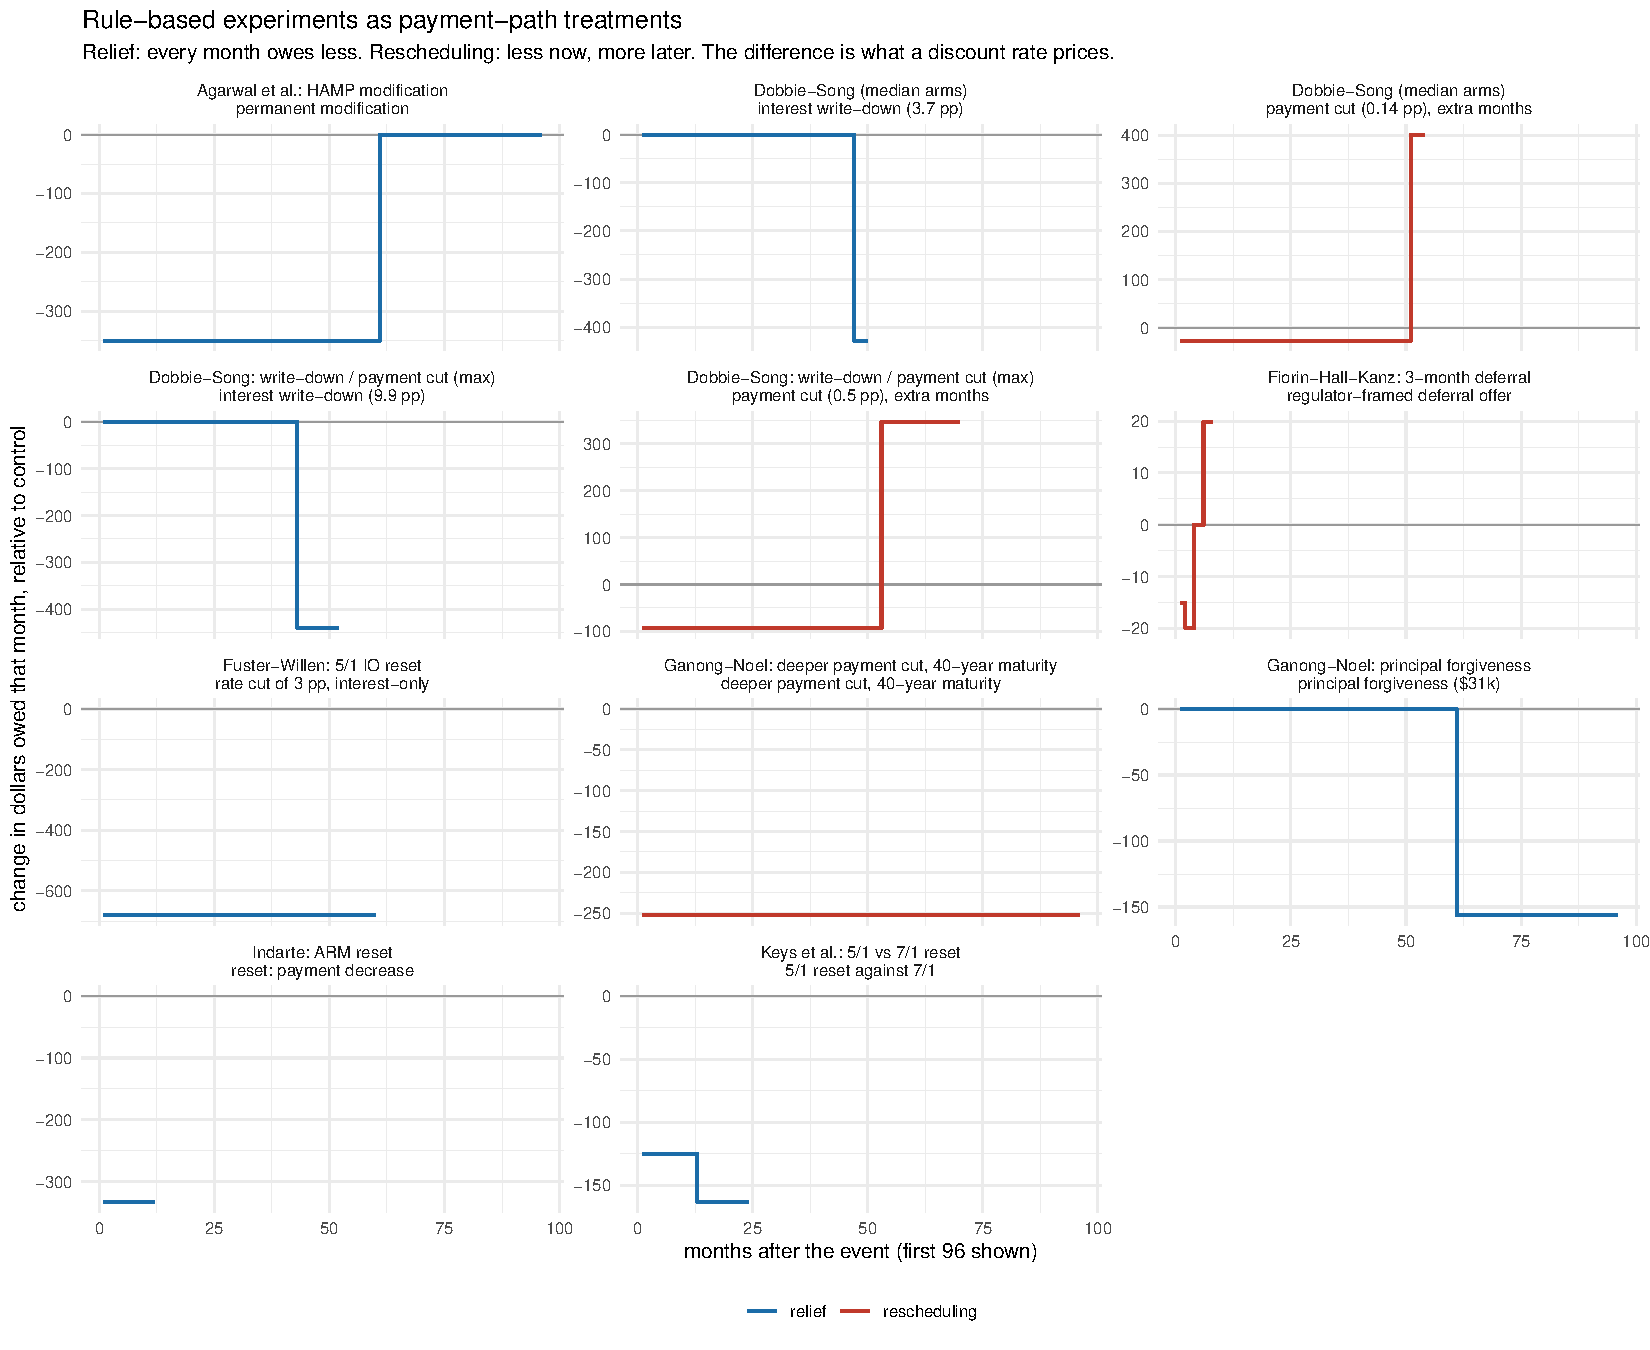
\includegraphics[width=\textwidth]{figures/fig_ledger_paths.pdf}
\begin{minipage}{0.95\textwidth}
\small \textit{Notes:} Each panel is one treatment arm: the change in dollars owed in each month after the event relative to the study's control (first 96 months shown). Blue: relief, every month owes less. Red: rescheduling, less now and more later. The studies shown are those of Table \ref{tab:experiments}. Source: \texttt{external/experiments\_paths.csv}.
\end{minipage}
\end{figure}

\begin{figure}[ht]
\centering
\caption{What each pair of arms says about the discount rate, and the near-horizon response across settings}
\label{fig:ledger_rho}
% replication: Code/exhibits/make_ledger_figures.R, Code/exhibits/make_lambda_figure.R; results/experiments_rho.csv, external/experiments_estimates.csv
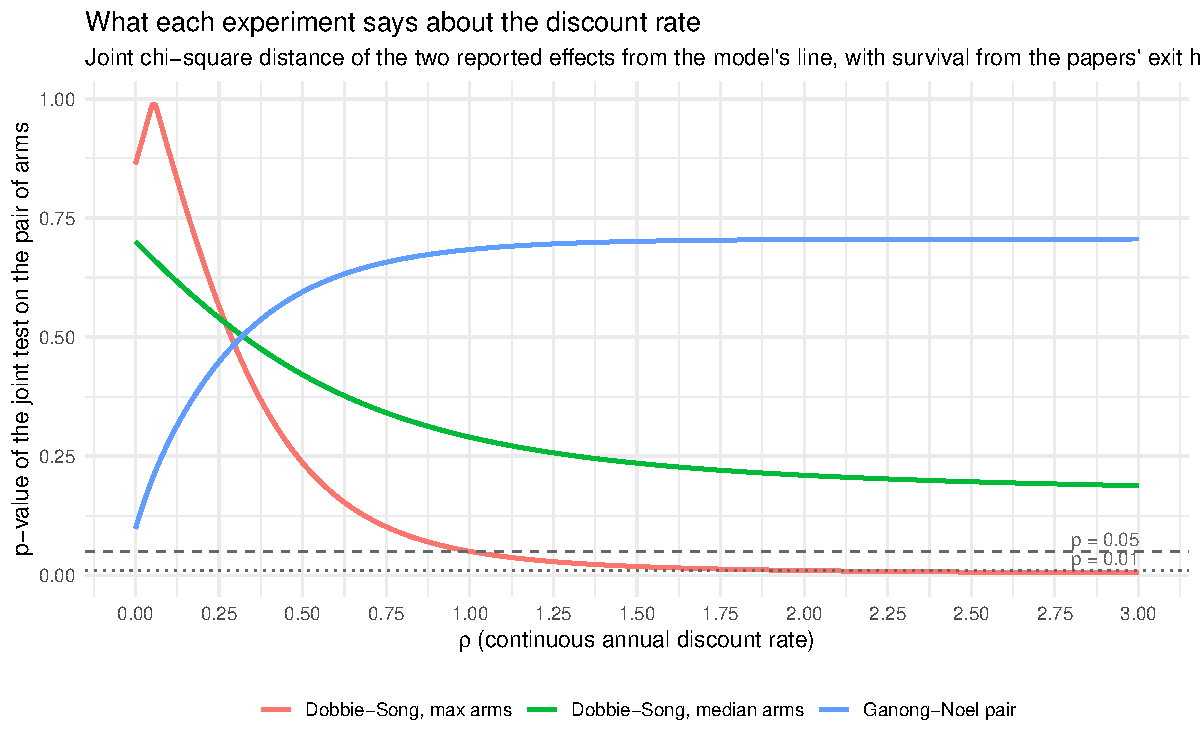
\includegraphics[width=0.8\textwidth]{figures/fig_ledger_rho.pdf}\\[0.5em]
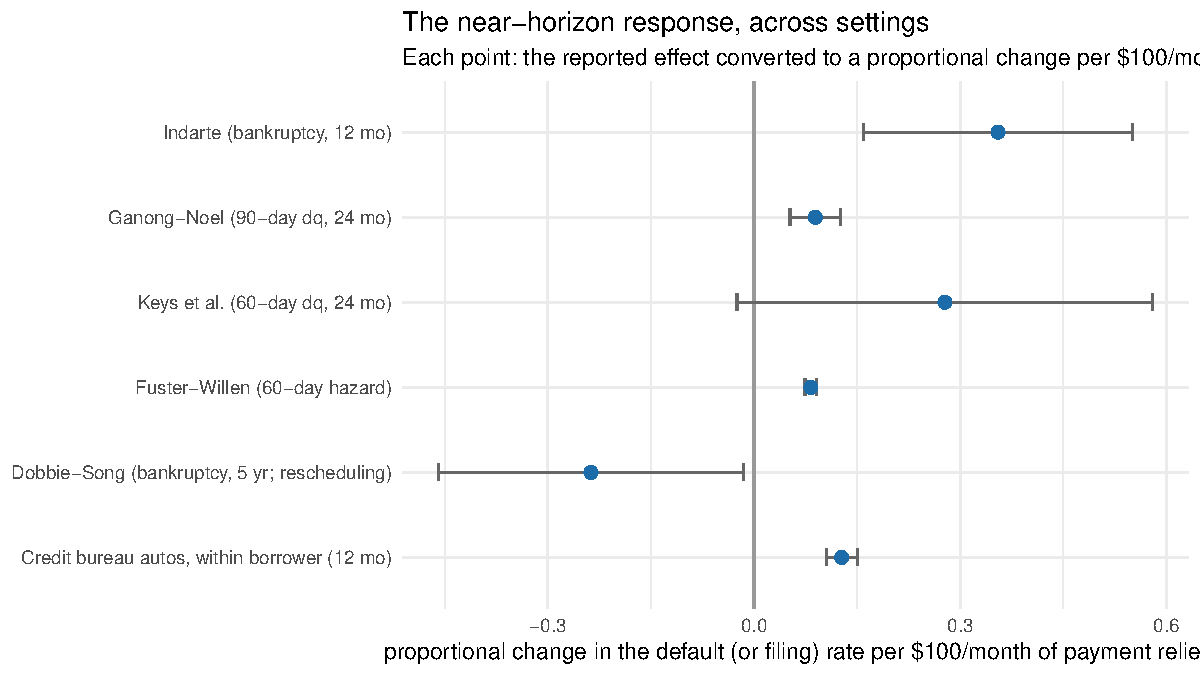
\includegraphics[width=0.8\textwidth]{figures/fig_ledger_near.pdf}\\[0.5em]
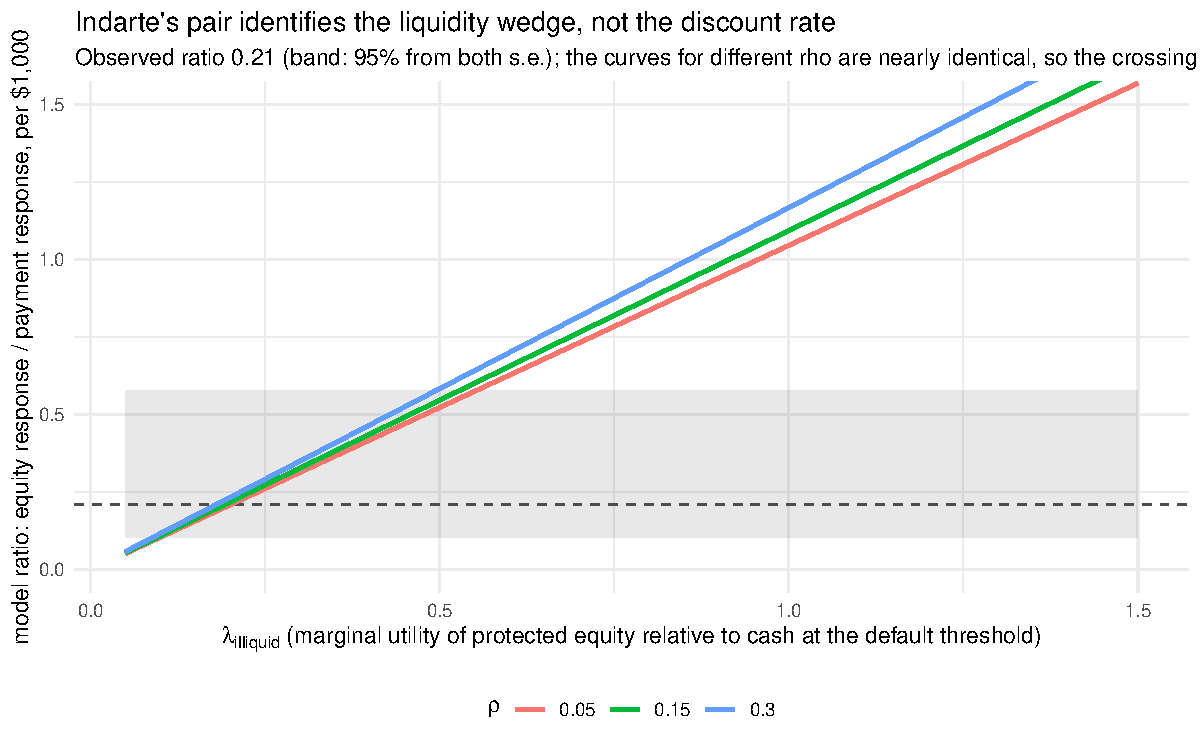
\includegraphics[width=0.8\textwidth]{figures/fig_ledger_lambda.pdf}
\begin{minipage}{0.95\textwidth}
\small \textit{Notes:} Upper panel: the $p$-value of the joint test of a pair of arms against the model, on the grid of $\rho$ from 0 to 3 (Section \ref{sec:mapping}; aggregated over each study's outcome window; survival from each study's exit hazards; the marginal-utility profile; the dashed and dotted lines are five and one percent). Middle panel: each study's reported response converted to a proportional change in the default or filing rate per \$100 a month of payment relief, with the credit-bureau within-borrower payment elasticity at a \$400 payment for comparison. Bottom panel: Indarte's pair, the ratio of the seizable-equity response to the payment response, as the model produces it for values of $\lambda_{\text{illiquid}}$ at three discount rates; the observed ratio crosses at about 0.2 whatever $\rho$ is.
\end{minipage}
\end{figure}



% appendix_strategies.tex: the identification graveyard: every design applied to these data, what it identifies, and why the ones that do not identify the rate fall short.
\section{The Identification Graveyard: Designs That Do Not Identify the Rate}\label{appendix:strategies}

The paper's estimate of the rate is the within-borrower one of Section \ref{sec:rate_people}; the across-borrower term margin adjusted for the penalty and selection is the check on it (Appendix \ref{appendix:ladder}), the rule-based experiments of Section \ref{sec:quasi} are the check on the sign and the horizon of the far-payment response, and the decline of the payment margin over the life of the loan is compared with the stopping model's own (Appendix \ref{appendix:mcliquidity}). Table \ref{tab:strategies} records every identification design applied to these data, with the object each identifies and, where it does not identify the rate, the reason, so that the estimates can be compared with the alternatives and a reader who prefers one of them can see what it costs. Appendix \ref{appendix:strategies:three} states in full the three objects in the bureau data that look as if they should reveal a discount rate and do not, and Appendix \ref{appendix:strategies:designs} states in full the eight design-based comparisons the paper uses.
\subsection{The record}

\begin{footnotesize}
\begin{longtable}{@{}p{0.21\textwidth}p{0.18\textwidth}p{0.42\textwidth}p{0.13\textwidth}@{}}
\caption{Identification strategies for the discount rate: the record}\label{tab:strategies}\\
% replication: the record of the designs, written from the memos and results named in each row; no generator
\toprule
Strategy & Object it would identify & What happened & Status \\
\midrule
\endfirsthead
\toprule
Strategy & Object it would identify & What happened & Status \\
\midrule
\endhead
\bottomrule
\endfoot
\multicolumn{4}{@{}l}{\emph{Estimating the discount rate from the default margins}} \\
Two separate logits on $\log m$ and $\log L$, ratio $\gamma_L/(\gamma_L+\gamma_m)$ & the payment-versus-total sensitivity of default & $\log L = \log m + \log T$, so each coefficient absorbs the other margin; the ratio is held near one half by construction (0.46--0.58 across eight fixed-effect menus) and its stability was a property of the construction & not an instrument for the rate \\
Joint regression, closed form $x/(e^x-1)$ with the full term & $\rho$ from the ratio of the two elasticities under exponential discounting & the marginal-utility ratio, survival in the loan and the balance penalty enter; on the model's own simulations the closed form overstates the ratio by 2.5--3$\times$, and the lifetime outcome reflects exposure & not an instrument for the rate \\
Fixed-window outcomes with the joint regression & the same ratio free of exposure & the ratio changes sign across windows (negative at six months, positive over the life) and across score deciles; the term margin is two channels plus exposure, not one & kept as a finding (Section \ref{sec:termmargin}) \\
\midrule
\multicolumn{4}{@{}l}{\emph{Instruments and designs for the term margin}} \\
Macro-rate instruments (Treasury lanes) & exogenous variation in the payment at a given term & failed the first-stage and exclusion gates; the control-function payment coefficient is negative & not an instrument for the rate \\
Lender size-menu instruments & exogenous variation in the term & lender-years with larger loans serve safer borrowers; the exclusion fails and one failure enters both instrumented coefficients & not an instrument for the rate \\
Leave-out lender-menu instruments (examiner design) & the same & lenders are not randomly assigned; kept as a diagnostic of the fixed-effect design (Appendix \ref{appendix:ivvalidation}) & diagnostic \\
Menu regression discontinuity at the 72-month amount cutoff & the effect of a rule-driven longer term at a fixed total & first stage strong but small (log $T$ rises by 0.01); second stage imprecise (elasticity $-2$ to $-8$, s.e. 1.3--4); score and income borderline continuous & imprecise \\
Difference estimator $\text{FE} - [\text{FE}(S) - \text{IV}(S)]$ under equi-confounding & the fixed-effect estimate corrected by its gap to the instrumented one where both exist & the pre-test problem; the gap is transportable only if invariant across groups, which is the criterion the specification search then imposes & measured; the invariance criterion of Appendix \ref{appendix:bridge} \\
Within-borrower fixed effects (two or more loans) & the margins free of every stable trait & the closest-to-causal profile the bureau offers; it does not remove the lender's private information at origination, which is time-varying & the validation target \\
Within-borrower ratio of the term response to the payment response, mapped through the window formula & the rate, with selection into contract length removed by design and the scale cancelled, conditional on the penalty channel having run off by twenty-four months & on 13.5 million borrowers with two or more auto loans (65 million loans): $0.02$ pooled, $0.11$ on average across score deciles; no gradient in score or income; a gradient in age; state ratios outside the formula's range (Section \ref{sec:rate_people}) & the paper's estimate \\
The same ratio by origination year, the borrower effect re-estimated inside each year & the rate by period & inside one year the borrower effect is identified only from borrowers with two auto loans in that year, and the ratio is at or above the formula's ceiling in every year; the period design interacts the elasticities with the period and identifies the borrower effect across years & replaced by the period design of Section \ref{sec:rate_people} \\
Servicer-transfer linking across furnisher keys & the exit hazard net of transfers, the formula's $h$ & a trade that moves to a new servicer exits under one key and reappears under another; matched on consumer and opening date, transfers are 15 percent of auto exits and 18 percent in the first year, and the net hazard is the one the estimates use (Appendix \ref{appendix:data}) & measured \\
Selection on observables (Oster) & the direction of selection on the term & higher score, shorter term: observed selection runs against the negative early-default coefficient & supporting \\
\midrule
\multicolumn{4}{@{}l}{\emph{Separating the channels of the term margin}} \\
Deficiency and recourse contrasts (state rules) & the balance-scaled penalty channel & confirmed pooled on the ten-percent extract ($+0.36$, s.e. $0.13$, at twelve months on autos; $+3.9$, s.e. $1.5$, on mortgages); on the one-percent panel with covariates there are 303 no-pursuit defaults and no power by group & pooled only \\
Full model inversion by group (optimal stopping, income process free) & $(\rho, \sigma)$ per group from the window profile and default rate & the model's term elasticities are a third the size of the observed ones and $\rho$ goes to the grid edges & not an instrument for the rate \\
Proposition \ref{prop:sensT} ratio with beliefs fixed (Appendix \ref{appendix:formula}) & $\rho$ per group given $\lambda$, survival and the penalty share & every profile is fitted, but $\rho$ and the penalty share are collinear across windows; the confidence set spans the grid; recovery on simulations is monotone but biased & needs an anchor \\
Contract-length bins as the extra dimension & separation of $\rho$ from the penalty share through the term & the exit hazard, not $\rho$, governs how the marginal payment's weight falls with the term; no separation & not an instrument for the rate \\
Charge-off amounts as the measured penalty base & the penalty channel's level and its shape over the loan's life, by group & measured with precision (elasticity to the payment 1.04; to the term 0.33 at six months rising to 1.79 after three years); under the first-order formula the measured shape makes both channels fall with the window while the observed ratio rises; the full model of Appendix \ref{appendix:mcliquidity} produces a rising ratio but at a third of the observed magnitude & the penalty shape is measured; the profile's rise is not explained \\
The equity margin on first mortgages: default against the house-price change since origination, against the payment (Section \ref{sec:mainresults}) & the ratio of a lump to a twenty-five-year stream, and its profile over loan age & 1.86 million mortgages, 191,581 events: elasticity $-2.5$, stronger without recourse, falling from $-5.9$ to $-1.1$ with age, convex in negative equity; in the model with a house, with i.i.d.\ income and a payment elasticity three times the measured one, the ratio to the payment response is between $-0.92$ and $-1.09$ at every rate, because the margin is the sale option (conditional on that calibration, Appendix \ref{appendix:persistent}) & measured; consistent with the model; not a rate \\
The term margin corrected rung by rung (Appendix \ref{appendix:ladder}) & $\rho$ from the ratio of the term to the payment response within twelve months, after the penalty and selection corrections & pooled charge-off: raw ratio 0.01 (rate near one), penalty correction to 0.81, selection correction to 0.39 (0.31), mapped to 0.04 with a set that spans the grid; ordering by group at the boundaries & measured; the check on the within-borrower estimate \\
\midrule
\multicolumn{4}{@{}l}{\emph{Timing variation inside the bureau}} \\
Deferred first payments and balloons & a rescheduling at a fixed balance & a few hundred auto loans; personal-installment deferrals are student-loan-like & unavailable \\
Pandemic forbearance & a rescheduling at scale & visible on mortgages only (1.3 percent at the 2020 peak), borrower-elected, and reported as current while in effect & not rule-based \\
Movers (place versus person) & the share of default variation due to place & answers its own question (slope 0.075, s.e. 0.013); it is not a discount-rate instrument & supporting \\
\midrule
\multicolumn{4}{@{}l}{\emph{What identifies $\rho$}} \\
Rule-based experiments, mapped through Proposition \ref{prop:sensT} (Section \ref{sec:quasi}) & $\rho$ for the populations the experiments treat & rescheduling against write-down fits best at zero and, aggregated over its five-year window, accepts $[0, 1.20]$ at five percent; the ARM resets anchor the near-horizon response; the forgiveness-versus-reduction pair is uninformative alone & measured; the check on the sign and the horizon \\
The payment margin over the life of the loan on the estimation sample & the run-off of the remaining payments' weight, by group & the run-off was large (the elasticity fell by two thirds over the contract); the sample's last-payment field, which reached the merged file through a separate charge-off extraction, dates the same cohorts' charge-offs three times as often in the first six months as the monthly panel does and a third as often late, so the profile was an artifact of default dating & not used; the monthly panel dates defaults from ratings \\
The payment margin over the life of the loan on the monthly panel, mapped through the first-order formula & the same, with survival and the marginal-utility ratio held constant & measured with standard errors of 0.02 over seven loan-age bins on 7.6 million loans; on the structural model's own simulations the formula attributes a run-off that the default option produces at any $\rho$ to a high $\rho$ (Appendix \ref{appendix:mcliquidity}), so the formula is not the mapping & measured; mapped through the model \\
The same profile, compared with the model's own run-off (Appendix \ref{appendix:mcliquidity}) & the set of rates at which the model reproduces each group's profile shape & the set spans the grid in nearly every group: the run-off validates the stopping problem and does not pin the rate & measured; not an instrument for the rate, by the option \\
\midrule
\multicolumn{4}{@{}l}{\emph{Timing variation inside the bureau}} \\
Adjustable-rate resets, 2004--08 originations, found from the payment path (Appendix \ref{sec:armreset}) & $D(\tau)\lambda$ at one to twelve months from the anticipation of a reset & 88,151 payment changes at hybrid reset ages, of which 9,224 are rate changes by the amortization identity and the rest escrow re-analyses, interest-only loans, recasts and closing trades; the index moved by less than 0.2 points across the 2010--13 reset years (first-stage $F$ below two); delinquency rises before a larger coming cut in every sample, a sign no discount function produces; 1,066 events on the clean cuts & the classification method and the pre-reset sign; no rate \\
The reset-type contrast: five-year against seven-year hybrids of the same vintage at the five-year reset month & the same, with vintage-specific trends removed & the pre-reset sign is the same within type, and the clean sample is too small to split & not built \\
The October 2023 student-loan payment resumption as a cross-loan experiment (Appendix \ref{sec:studentloan}) & the anticipation response at four to one months and the at-date response of auto delinquency to a known bill on another account, by its size & 438,311 holders, 743,487 auto loans, 17,711 events; the coefficient per \$100 of bill is negative in every month from March 2023, before the statute, through 2025 (composition of the exposure); the change at the bill is $-2.8$ ($0.6$) against $+5.9$ for an enforced payment of that size; half the bills unpaid and none reported delinquent for a year & measured; not an enforced payment, so not the design's premise \\
The same design on the enforced payments after May 2025 & the same & the coefficients from May to December 2025 do not separate from the preceding drift & open as the panel lengthens \\
Adjustable-rate resets in the ten-percent archive & the same as the one-percent resets with ten times the loans & the archive is observed twice a year through 2017, which does not resolve a monthly anticipation profile & not built, by the data's frequency \\
HAMP step-ups, 2014--19 & the same, from rule-fixed annual payment increases on modified loans & the amortization identity finds 2,478 rate rises of one half to one and a half points on loans below 4.5 percent in 2013--18, 69 of them twelve months after a previous one: fewer events than the reset cuts & too few events \\
Balloon payments, all families (\texttt{balloonpaymentamount}, \texttt{dateballoonpaymentdue}) & $D(\tau)\lambda$ at one to five years from the approach of a contractual lump sum & about 2,000 open auto and 3,000 dated mortgage balloons per one-percent snapshot, a few hundred delinquency events over their lives & too few loans \\
Credit-card promotional expirations & $D(\tau)\lambda$ at twelve to eighteen months for revolvers at the minimum & revolving trades' monthly minimum payments & not built \\
Contract-length bins as step responses within borrower (the discount kernel from the term margin) & the weight on payments at each added lag, from the step in default across contract lengths & steps are not monotone in the lag: the standard terms of 60 and 72 months stand above 48, 66 and 84 at every horizon, so the bins measure which product and lender the borrower took, not the weight on the added payments; the one clean pair, 60 against 72 months, is one point, not a curve & menu effects; not a kernel \\
Credit-card promotional-rate expirations & $D(\tau)\lambda$ at twelve to eighteen months from a payment increase fixed by the card agreement & delinquency rises by $0.033$ percentage points per one percent of the coming payment increase in the months before expiry and does not move at expiry; without cards of the same age without a promotion the anticipation cannot be separated from card age & measured; no control group \\
Pandemic forbearance exits & the rate at long horizons from deferred balances against repayment plans & narrative codes and payment paths & not built \\
\end{longtable}
\end{footnotesize}

Three lessons organize the table. First, a ratio of two coefficients on the same outcome cancels only symmetric confounding; every mechanism found loads on one margin, so sharing the outcome removed nothing. Second, the term margin across borrowers is the wrong instrument for a discount rate in these data: it bundles a preference channel bounded above by one, a balance-scaled penalty whose shape is measured, and a component that rises with the window and with the score, which neither channel produces at the observed magnitude; screening at origination on the lender's private information, whose predictive power decays, is the candidate the within-borrower design cannot remove. Third, what identifies a discount rate without a model of the penalty is variation in the timing of payments at a fixed balance, which the bureau does not contain on auto loans and the rule-based experiments do; the bureau's within-borrower ratio gives a rate with selection removed by design and the penalty channel assumed to have run off by twenty-four months, and the bureau's other contribution is the population-scale measurement of the objects the formula uses, and their heterogeneity across people and time.

\subsection{The three objects that do not identify the rate, in full}\label{appendix:strategies:three}

Three objects in the credit-bureau data look as if they should reveal a discount rate and do not, each for a reason that is itself a result of the theory. This subsection states each in full.

\paragraph{The response to a payment due now against payments due later cannot separate impatience from the present-payment premium.} Every response of default to a payment at date $s$ has the weight $D(s-1)Q_s\lambda$, and under quasi-hyperbolic discounting the present-bias parameter and the marginal-utility ratio appear in that weight only as the product $\beta\lambda$ (Theorem \ref{thm:betalambda}). This is not a limitation of a particular design: any experiment that moves a payment due now against payments due later, whether a payment holiday, a step-up, a rescheduling or the run-off of a contract, produces ratios that depend on $(\beta, \lambda)$ through their product, so the same data are consistent with a fully present-biased borrower whose marginal utility is the same in every state and with a time-consistent borrower who is liquidity-constrained at the margin. What separates them is a comparison of two dollars at the same date valued at different marginal utilities, a liquid dollar and an illiquid one, which the cash-on-hand and seizable-equity responses of \citet{indarte_moral_2023} provide (Corollary \ref{cor:separate}). The paper therefore measures the premium from that pair, uses the profile of equation \eqref{eq:lambda_p}, through Indarte's $0.2$, for the experiments' populations and for the bureau's groups, and reports the exponential rate beyond the first payment.

\paragraph{The response to the contract's length across borrowers cannot identify the rate on its own.} A longer contract at a fixed payment adds far payments, which a patient borrower weighs more heavily, but it also raises the balance the lender can pursue after default and the number of months in which a default can occur. Proposition \ref{prop:termmargin} writes the term response as the sum of the three: a preference channel bounded above by one in units of the payment response, a balance-scaled penalty channel that is negative and discounted at the contract rate, and, for lifetime outcomes, exposure; across borrowers it adds selection into contract length. Two features of the data show that the penalty and exposure dominate at short horizons. Within lender, place, year and score-by-income cell, a longer contract at a fixed payment lowers early delinquency for low-score borrowers and raises it for high-score borrowers, and the ratio of the term response to the payment response exceeds one above the fifth score decile, outside the preference channel at any rate (Section \ref{sec:termmargin}); and the early effect is weaker, by a third at twelve months on auto loans and by roughly half on mortgages, in the states whose laws bar the lender from pursuing the balance after repossession. The across-borrower term margin is reported as a finding about the cost of default, and it is mapped to a rate only after the penalty and selection are subtracted (Appendix \ref{appendix:ladder}); within borrower, with selection removed by design, it is taken at twenty-four months conditional on the penalty channel having run off (Section \ref{sec:rate_people}).

\paragraph{The run-off of the payment margin over the life of the loan is not mapped to a rate.} As a loan ages the remaining payment stream shortens, and a first-order formula, with survival and the premium held constant, would have the response to the payment decline at a rate governed by $\rho$. The optimal-stopping model says otherwise. A borrower who continues buys one period of standing plus the option to reconsider (Proposition \ref{prop:interiorT}), so the far payments enter her decision only with the weight of the states in which she will still be paying them, and when default is a threshold crossing in income that weight is small at every rate. On the model's own simulations, calibrated to the sample's default rate with exits at the measured hazard, the run-off ratio is between $0.77$ and $0.82$ at every rate from zero to $1.2$ (Appendix \ref{appendix:mcliquidity}), and the first-order formula applied to those simulations returns rates near $3$ at true rates of $0.03$ to $0.10$. The measured run-off, $0.75$ under the charge-off definition and $0.67$ under the ninety-day definition, lies below that range as a point estimate, and the 95 percent bands of the observed profiles overlap it in nearly every group (Section \ref{sec:mainresults}). The result is conditional on the calibration. The model reaches the sample's default rate only with a payment elasticity near five against the data's $0.45$ and with $0.93$ of lifetime default in the first year against the data's $0.13$; a version with a persistent income process, calibrated to the lifetime rate and to the first-year share, matches the timing of default, keeps the same elasticity at every persistence and dispersion, and has a run-off that is again insensitive to the rate but at a level of $0.2$ with a profile that declines from the first year, against the data's flat profile (Appendix \ref{appendix:persistent}). Neither version reaches the level of the payment margin, so the run-off is not used for the rate in either direction: it is not mapped through the first-order formula, and the model's insensitivity result is not a demonstration that the data's run-off contains no information about the rate.

\subsection{The design-based comparisons in full}\label{appendix:strategies:designs}

An estimate is design-based when the variation it uses is fixed by something the borrower does not choose, a state law, a statute, the date at which a neighbor bought a house, or when the borrower herself is held fixed, so that the comparison is between two of her own loans; an estimate is fixed effects plus adjustment when it compares loans that are alike on what the data record and is causal under the assumption of Section \ref{sec:identification}. The eight design-based comparisons are the following.

\begin{enumerate}
\item \emph{The payment margin within borrower.} The design compares a borrower's default on one of her auto loans with her default on another, within origination-year cells, on the ten-percent archive. Charge-off within twelve months responds to the monthly payment with an elasticity of $0.44$ (standard error $0.005$), and within twenty-four months $0.53$ ($0.003$) (Table \ref{tab:main_margins}, lower panel). This is the response of default to the payment due now for a fixed person. What the design leaves is what changed about her between the two loans that the lender saw and the cell does not record; Table \ref{tab:strategies} names that as the one confounder the within-borrower design cannot remove.

\item \emph{The term margin within borrower, by score.} The same design, with the contract's length at a fixed payment as the treatment, run decile by decile on the multi-loan borrowers with a score, the decile fixed by the borrower's first score, within borrower and origination-year cells (Table \ref{tab:within_by_group}). Within twenty-four months the elasticity is $0.30$ ($0.01$) pooled and between $0.19$ and $0.43$ across deciles, and its ratio to the within-borrower payment elasticity, the paper's sufficient statistic, is between $0.32$ and $0.53$ in every decile with standard errors from $0.02$ to $0.10$ (Table \ref{tab:rho_within}); within twelve months the elasticity is $-0.31$ ($0.01$). Across borrowers, within the same lender-year cells, the same elasticity runs from $-0.39$ in the bottom decile to $1.21$ in the top, so the whole gradient is selection into contract length, positive where lenders screen with maturity and negative where prime borrowers choose long terms for themselves \citep{hertzberg_screening_2018}. On personal installment loans the same design gives $0.28$ ($0.01$) at twenty-four months, and $0.30$, $0.29$ and $0.19$ by score tercile. The response of default to payments added at the end of a contract, net of every stable trait, is the same for every score in two loan families, and the selection correction of Appendix \ref{appendix:ladder} is measured, with a standard error of $0.01$ pooled, rather than assumed.

\item \emph{The deficiency-judgment contrast.} In sixteen states the law bars the lender from pursuing the unpaid balance after repossession on a loan below a threshold. The design compares auto loans below the threshold in those states with loans of the same size in states without a bar, within zip3-by-year cells (Table \ref{tab:term_deficiency}). Where the balance cannot be pursued, the term elasticity of default within twelve months is higher by $0.36$ ($0.13$), and within thirty-six months by $1.02$ ($0.27$); on mortgages, using recourse and non-recourse states, the difference is $3.9$ ($1.5$) at twelve months. This is the penalty channel of Proposition \ref{prop:termmargin} measured at its deficiency part: the cost of default rises with what is owed, by law, and a longer contract at the same payment lowers early default for that reason.

\item \emph{The equity margin.} Two households in the same zip code in the same quarter who bought their houses in different years hold different equity because prices moved between the two purchases; with zip-by-quarter and origination-year effects, the comparison is between origination cohorts under the same local conditions (Table \ref{tab:equity_margin}). The quarterly hazard of first 90-day delinquency responds to the log house-price change since origination with a coefficient of $-2.23$ ($0.09$), times one hundred, an elasticity of $-2.54$; the ratio of that response to the payment response is $-1.71$ ($0.07$), and it is $-2.38$ ($0.16$) in the states without deficiency judgments against $-1.54$ ($0.09$) with them. The response falls with the loan's age, from an elasticity of $-5.90$ in the first three years to $-1.07$ after seven, and the hazard is convex in negative equity, adding $3.9$ percentage points per quarter, four and a half times the base, once the price has fallen by half. These are the signatures of a walk-away decision and its dependence on recourse. The model with a house, with i.i.d.\ income and a payment elasticity of $4.7$ to $5.5$ against the measured $1.5$, returns a ratio between $-0.92$ and $-1.09$ at every rate (Table \ref{tab:equity_model}; the calibration's limits are those of Appendix \ref{appendix:persistent}), so the margin is consistent with the stopping problem and is not used for the rate.

\item \emph{The adjustable-rate resets.} The amortization identity finds, without a contract flag, $6{,}348$ rate cuts at hybrid reset ages among $429{,}078$ payment changes on 2004--08 first mortgages, with loan and vintage-by-calendar-month effects (Appendix \ref{appendix:timing}), and $11{,}859$ cuts when only the amortization before the cut is required. On that larger sample the response of first 90-day delinquency at the cut is $-0.50$ ($0.36$) per unit of log payment, times one hundred, and in the four months before it $-0.47$ ($0.13$): delinquency is higher before a larger coming cut. The sign is one that no discount function produces, and with the index flat across the reset years and $1{,}066$ events, no rate is estimated from this population (Section \ref{sec:mainresults}).

\item \emph{The student-loan resumption.} A statute fixed the date on which student-loan payments resumed, and the size of each bill was fixed by the student loan; the design follows auto default on the same consumer (Appendix \ref{appendix:timing}). The coefficient of first 90-day auto delinquency on the resumed bill, per hundred dollars, changes by $-2.8$ ($0.6$), in units of $10^{-5}$ per month, between the months before the statute and the months of the first bills, against $+5.9$ for an enforced payment of that size; the response is measured to within $\pm 1.4 \times 10^{-5}$, two percent of the base hazard, and is not positive at any horizon in any group. Auto default does not respond to a bill on another account that half of its recipients did not pay and that had no consequence for a year (Section \ref{sec:mainresults}).

\item \emph{The menu regression discontinuity.} Lenders admit a 72-month contract only above a loan-amount cutoff, and the design compares loans just above with loans just below it, within lender-year, at bandwidths of two to five thousand dollars. The log contract length rises by $0.011$ ($0.001$) at the cutoff, a first stage with an $F$ statistic near $200$ but small; the implied elasticity of default within twelve months to the term at a fixed total is $-2.6$ ($2.0$) at the middle bandwidth and $-2.1$ ($1.3$) at the widest. A longer term at a fixed total is a lower payment, and default falls, which is the sign of the payment margin; the estimate is not distinguishable from zero and is not used.

\item \emph{Movers.} Borrowers whose three-digit zip code changes between two of their loans identify how much of the geographic gradient in default is the place: the change in a mover's own default, regressed on the change in the stayers' default rate between destination and origin, has a slope of $0.075$ ($0.013$) over the life of the loan (Table \ref{tab:person_place}). The geography of Section \ref{sec:heterogeneity} is composition to that extent, and this is not a discount-rate object.
\end{enumerate}


% appendix_iv_validation.tex: Using an instrument observed on a subsample to
% validate a fixed-effects design (2026-09-03).
\section{An Instrument on a Subsample and the Design for the Full Sample}\label{appendix:ivvalidation}

This appendix states when an instrument that exists on a subsample $S$ of the data justifies a fixed-effects design on all of it, and how the standard errors should be computed. The argument is linear; the logit case follows by the same steps on the score.

\subsection{Setup}
For unit $i$ let $y_i = \tau x_i + c_i + e_i$, with $x_i$ the regressor of interest, $c_i$ an unobserved confounder correlated with $x_i$, and $e_i$ independent noise. A fixed-effects design $F$ partitions units into cells; $M_F = I - P_F$ is the within-cell projection. An instrument $z_i$ with $\mathbb{E}[z_i c_i \mid F] = \mathbb{E}[z_i e_i \mid F] = 0$ is observed only on $S$.

\subsection{What the fixed-effects estimator estimates}
On any sample $A$,
\begin{equation}
\hat\tau_F(A) = \tau + \underbrace{(x'M_F x)^{-1}x'M_F c}_{b_F(A)} + (x'M_F x)^{-1}x'M_F e,
\end{equation}
so the bias $b_F(A)$ is the within-cell regression coefficient of the confounder on $x$ in sample $A$. When cells nest within $S$ and $S^c$, the full-sample bias is the variance-weighted average
\begin{equation}\label{eq:biasavg}
b_F(\text{Full}) = w_S\, b_F(S) + (1 - w_S)\, b_F(S^c), \qquad w_S = \frac{x_S' M_F x_S}{x'M_F x}.
\end{equation}
The instrument identifies $\tau$ on $S$. A design selected because $\hat\tau_F(S) \approx \hat\tau_{IV}(S)$ and then applied to the full sample is unbiased if and only if $b_F(S^c) = 0$ given $b_F(S) = 0$. The difference estimator
\begin{equation}\label{eq:diffapp}
\hat\tau^{D} = \hat\tau_F(\text{Full}) - \big[\hat\tau_F(S) - \hat\tau_{IV}(S)\big]
\end{equation}
is unbiased if and only if $b_F(S^c) = b_F(S)$. The second condition contains the first as the case $b_F(S) = 0$; it does not require the design to be exactly right on $S$, and it uses the instrument as a level rather than as a test.

\subsection{The assumption}
Write $c = c_F + \eta$ with $c_F$ measurable with respect to the cells, so $M_F c = M_F \eta$. If the conditional law of $(x, \eta)$ given the cell is the same in $S$ and $S^c$, then $b_F(S) = b_F(S^c)$. This is unconfounded location in the sense of \citet{hotz_predicting_2005} and equi-confounding in the sense of \citet{li_identification_2024}: membership in $S$ is independent of the residual confounding mechanism given the cells, while cell means, effect sizes, and the distribution of $x$ across cells may differ. It is the weakest condition under which either procedure is consistent, and under it the difference estimator dominates selection: it needs no choice among designs and inherits no pre-test distortion \citep{leeb_model_2005, guggenberger_impact_2010}. A testable implication is that the estimated bias $\hat\tau_F(S) - \hat\tau_{IV}(S)$ is constant across groups of units within $S$; \citet{angrist_leveraging_2017} apply the same check to the bias of value-added estimates across schools with and without lotteries. Effects for groups that exist only in $S^c$ are identified only under the assumption itself or under a parametric bias function estimated on $S$ and extrapolated \citep{kallus_removing_2018}.

\subsection{Standard errors}
The three pieces of \eqref{eq:diffapp} share the observations in $S$, so
\begin{equation}
\mathrm{Var}(\hat\tau^{D}) = \mathrm{Var}\,\hat\tau_F(\text{Full}) + \mathrm{Var}\big[\hat\tau_F(S) - \hat\tau_{IV}(S)\big] - 2\,\mathrm{Cov}\big(\hat\tau_F(\text{Full}),\, \hat\tau_F(S) - \hat\tau_{IV}(S)\big),
\end{equation}
which a cluster bootstrap over the units of instrument variation, stratified by $S$, estimates directly; this is the variance of the prediction-powered estimator of \citet{angelopoulos_prediction_2023}. It exceeds the variance of the fixed-effects estimate alone by the variance of the estimated bias.


\subsection{The instruments, and why they fail}\label{appendix:failedinstruments}

For lender-years with at least fifty originations, 97 percent of loans, two leave-one-out instruments exist: the lender's share of long-term originations in the year, which shifts $T$ through the maturity menu \citep{argyle_monthly_2020, hertzberg_screening_2018}, and the lender's mean log loan size, which shifts $m$ given $T$ through the size menu. The two-stage least-squares payment coefficient on that subsample is negative, the opposite sign to every payment response in the paper, including the within-borrower estimate and the rule-based experiments (Table \ref{tab:identification}). Lender-years with larger loans serve safer borrowers, so the size-menu instrument moves the payment together with unobserved risk and the exclusion restriction fails; the bias the instrument would measure differs across regions, where a valid instrument would give one value. The size-menu instruments therefore do not identify the payment margin, and the difference estimator of this appendix, which would transport an instrument's information from the subsample to the full sample, has nothing valid to transport. The fixed-effects estimate of the payment margin stands on the institutional argument and the sign argument of Section \ref{sec:identification}, its agreement with the within-borrower estimate, and its agreement with the published payment responses at the same margin (Table \ref{tab:benchmark}).

\subsection{The balance held fixed: the rate margin}\label{appendix:ratemargin}

The paper's payment margin moves the balance with the payment at a fixed term. With $\log m$, $\log T$ and $\log L$ all in the regression, the amortization identity $m = L\,r/(1 - (1+r)^{-T})$ ties the three, and the only remaining source of variation in any one of them at fixed values of the other two is the contract rate $r$: both coefficients then measure the response of default to the rate, and within a borrower the rate is the lender's price of that loan's risk at that origination. On the multi-loan borrowers of the ten-percent archive the within-borrower payment elasticity with the log balance held fixed is $1.99$ at twenty-four months against $0.53$ with the balance moving, and the term elasticity $1.62$ against $0.30$; the ratio of the two, near $0.8$, sits above the formula's ceiling in every group and is a ratio of two rate responses rather than a far-to-near payment weight. The balance-fixed estimate is the bureau's counterpart to the published quasi-experiments that move a payment through the rate, and Table \ref{tab:benchmark} reports it beside them; the paper's own margin stays the payment with the balance moving, the cleanest payment variation the bureau offers within borrower.

\subsection{The estimate on the auto panel}\label{appendix:ivvalidation:auto}

Section \ref{sec:identification} states the assumption under which the fixed-effects estimate of the payment margin is causal and reports that the size-menu instruments give the opposite sign. This subsection reports the difference estimator applied to the auto panel. The instruments are constructed on the zip3-by-origination-year cells of the covariate-matched extract, for lender-years with at least fifty originations, which hold 97 percent of loans: the lender's leave-one-out share of long-term originations in the year, which shifts $T$ through the maturity menu \citep{argyle_monthly_2020, hertzberg_screening_2018}, and the lender's leave-one-out mean log loan size, which shifts $m$ given $T$ through the size menu. On this subsample $S$ the two-stage least-squares estimate of $(\gamma_m, \gamma_T)$ is compared with the fixed-effects estimate on the same loans, and equation \eqref{eq:diffapp} corrects the full-sample fixed-effects estimate coefficient by coefficient. The estimator is consistent for the full-sample coefficients under equi-confounding, stated for this application as follows.

\begin{quote}
\emph{Equi-confounding.} Within a zip3-by-origination-year cell, the projection of the unabsorbed determinants of default on $(\log m, \log T)$ is the same for loans at large lenders as for loans at small lenders. Default rates, the sizes of the payment and term effects, and the distribution of contracts may all differ between the two groups; what may not differ is the within-cell relationship between contract terms and the risk the cell does not absorb.
\end{quote}

\noindent This is the assumption under which the instrument's information travels from the subsample to the rest of the data \citep{li_identification_2024, angrist_leveraging_2017}, and it is weaker than the assumption that large-lender loans are a random draw \citep{hotz_predicting_2005}. What it excludes is a confounder that operates only at small lenders: a pricing practice that ties the payment to unobserved risk in a way that large lenders' underwriting does not. Its testable implication is that the estimated bias, $\hat\gamma^{FE}(S) - \hat\gamma^{IV}(S)$, is the same across groups of loans that exist within $S$. Table \ref{tab:identification} reports the estimated bias for the subsample as a whole and for the groups within it that hold enough instrument variation to estimate it separately, the bottom income quartile and the South and West census regions; the standard errors on every row come from a cluster bootstrap over lenders, stratified by subsample, so that the covariance among the three pieces of equation \eqref{eq:diffapp} enters the corrected estimate.

The instruments are leave-out means, the construction of the examiner design \citep{kling_incarceration_2006, dobbie_targeted_2020}, with one difference that fixes where the argument can fail. Cases are randomly assigned to examiners; borrowers are not randomly assigned to lenders. The exclusion restriction therefore requires that, within a cell and within a lender, the year-to-year movement of the lender's menu is unrelated to the unobserved risk of the borrowers it attracts. The failure to guard against is sorting: a lender that expands long maturities in a year in which it also reaches down the risk distribution. Three features of the design address it. Lender fixed effects remove the cross-lender association between menus and clienteles, so that only within-lender changes in the menu identify; Table \ref{tab:identification} reports the corrected estimate with and without them. The two instruments over-identify the two coefficients by one restriction; a violation common to both instruments escapes a test of that restriction, a violation specific to one does not. And a confounder that moves default through both margins in proportion, as a lender's overall reach down the risk distribution does, scales $\gamma_m$ and $\gamma_T$ together; only a confounder that acts on one margin and not the other moves their relative size, which is a narrower class than the class of confounders of either coefficient alone.

Table \ref{tab:identification} reports the result. The fixed-effects payment coefficient is $+0.122$ (standard error $0.044$, linear-probability units times 100) on all loans and $+0.107$ ($0.045$) on the subsample; the two-stage least-squares coefficient on the subsample is $-0.713$ ($0.293$), so the difference estimator returns $-0.698$ ($0.292$), and with lender effects $-0.912$ ($0.502$). The instrument-corrected payment coefficient has the opposite sign to the fixed-effects one and to every payment response in the paper, including the within-borrower estimate and the rule-based experiments. The reason is in the instruments. Lender-years with larger loans serve safer borrowers, so the size-menu instrument moves the payment together with unobserved risk and the exclusion restriction fails; the estimated bias in Panel B, which equi-confounding requires to be the same across groups, is $0.42$ in the South and $1.49$ in the West. The size-menu instruments therefore do not identify the payment margin (Appendix \ref{appendix:strategies}), and the paper's estimate is the fixed-effects one, defended as Section \ref{sec:identification} states. Two limits of the difference estimator remain in any application of it to these data. Groups of borrowers that exist only at small lenders receive a correction estimated at large lenders; for them equi-confounding is an assumption without a test. And the instruments identify the response of compliers to the lender's menu, whereas the fixed-effects coefficients weight every loan by its within-cell variance; the bias term in \eqref{eq:diffapp} absorbs the difference between these two averages along with any confounding, which is the cost of using the instrument as a level rather than as a test.

\begin{table}[ht]
\centering
\caption{The payment margin: fixed effects, instruments, and the corrected estimate on the large-lender subsample}
\label{tab:identification}
\resizebox{\textwidth}{!}{\begin{tabular}{lrrrr}
\toprule
Design & $\gamma_m$ & (s.e.) & $\gamma_T$ & (s.e.) \\
\midrule
\multicolumn{5}{l}{\emph{Panel A: default within twelve months (linear probability coefficients $\times 100$)}} \\
Fixed effects, all loans & 0.122 & (0.044) & -0.836 & (0.188) \\
Fixed effects, large-lender subsample & 0.107 & (0.045) & -0.794 & (0.206) \\
Two-stage least squares, subsample & -0.713 & (0.293) & -0.717 & (0.485) \\
Difference estimator & -0.698 & (0.292) & -0.759 & (0.474) \\
Fixed effects, all loans, with lender effects & 0.163 & (0.026) & -0.093 & (0.095) \\
Fixed effects, subsample, with lender effects & 0.169 & (0.026) & -0.070 & (0.101) \\
2SLS, subsample, with lender effects & -0.906 & (0.502) & 1.749 & (0.821) \\
Difference estimator, with lender effects & -0.912 & (0.502) & 1.725 & (0.819) \\
\midrule
\multicolumn{5}{l}{\emph{Panel B: the estimated bias $\hat\gamma^{FE}(S) - \hat\gamma^{IV}(S)$ by group ($\times 100$)}} \\
All loans in the subsample & 0.809 & (0.037) & -0.052 & (0.045) \\
Score decile 1 & 1.021 & (0.242) & -0.528 & (0.214) \\
Score decile 2 & 0.426 & (0.149) & 0.114 & (0.159) \\
Score decile 3 & 0.512 & (0.094) & -0.085 & (0.109) \\
Score decile 4 & 0.294 & (0.063) & 0.142 & (0.092) \\
Score decile 5 & 0.250 & (0.044) & -0.140 & (0.058) \\
Score decile 6 & 0.075 & (0.024) & -0.067 & (0.039) \\
Score decile 7 & 0.065 & (0.023) & -0.042 & (0.030) \\
Income quartile 1 & 1.147 & (0.125) & 0.043 & (0.114) \\
Income quartile 2 & 0.686 & (0.055) & -0.640 & (0.059) \\
Income quartile 3 & 0.171 & (0.030) & -0.244 & (0.033) \\
Income quartile 4 & 0.059 & (0.015) & -0.056 & (0.020) \\
Region NE & 0.635 & (0.061) & -0.324 & (0.062) \\
Region MW & 0.248 & (0.054) & -0.074 & (0.085) \\
Region S & 0.888 & (0.076) & -0.001 & (0.085) \\
Region W & 1.188 & (0.064) & 0.209 & (0.095) \\
\bottomrule
\end{tabular}
}
\vspace{0.5em}
\begin{minipage}{0.95\textwidth}
\small \textit{Notes:} Rows report the coefficients on $\log m$ and $\log T$ for default within twelve months on the covariate-matched extract: fixed effects on all of its loans, fixed effects and two-stage least squares on the subsample of lender-years with at least fifty originations, the estimated bias, and the difference estimator of equation \eqref{eq:diffapp}, with and without lender fixed effects; standard errors from a cluster bootstrap over lenders stratified by subsample. The lower panel reports the estimated bias for the subsample and for the groups within it with enough instrument variation to estimate it separately.
\end{minipage}
% replication: Code/identification/I2c_margins_iv.R, I2d_difference_estimator.R
\end{table}

\paragraph{The within-borrower specification with lender-year cells.} Every within-borrower estimate in the paper absorbs borrower and origination-year effects, so that a borrower's contracts are compared across lenders at the same date. The same regression on the same loans with lender-year in place of origination-year effects, which holds the lender's menu fixed as well as the borrower, gives a payment elasticity of $0.51$ ($0.005$) within twelve months, $0.57$ ($0.003$) within twenty-four and $0.47$ over the life of the loan, and a term elasticity of $-0.19$ ($0.01$), $0.00$ ($0.01$) and $0.42$ ($0.01$): the twelve-month term response and the lifetime response survive, and the twenty-four-month response, which the origination-year specification puts at $0.30$, is absent. Within one lender's menu in one year the contract length varies with the amount financed and the borrower's screening by that lender \citep{hertzberg_screening_2018}, so the two specifications compare different pairs of contracts, and the paper reports both. Replication: \texttt{Code/identification/I6\_within\_person.R}, rows \texttt{borrower + lender-year} of \texttt{results/identification\_within\_person.csv}.



\section{Inference}\label{appendix:delta_method}

Three objects are reported with standard errors in the paper. The elasticities of equation \eqref{eq:main_reg} are linear-probability coefficients divided by the window's default rate, with standard errors clustered by lender-year (the level at which the menu of contracts is set) and reported by zip3 and by state in the replication file; the ratio of the term elasticity to the payment elasticity in Section \ref{sec:termmargin} uses the delta method on the two coefficients' joint covariance from the same regression, $\mathrm{se}(\gamma_T/\gamma_m)^2 = \sigma_T^2/\gamma_m^2 + \gamma_T^2 \sigma_m^2/\gamma_m^4 - 2\gamma_T \sigma_{Tm}/\gamma_m^3$; the same formula gives the standard error of the equity-to-payment ratio of Table \ref{tab:equity_margin} and, with the deficiency contrast's variance added to the term coefficient's, of the corrected ratio in the ladder of Table \ref{tab:bureau_ladder}, whose set of rates carries that standard error through the formula. The match of a group's run-off to the structural model's is a weighted least-squares comparison of the seven loan-age elasticities with the model's profile at each rate on the grid, with the level free; the set of rates reported in Table \ref{tab:runoff_shape} is the set whose objective lies within $3.84$ of the minimum, the $\chi^2(1)$ cut, and it can be one-sided. The estimates from the rule-based experiments in Section \ref{sec:quasi} test each pair of reported effects against the model's line on a grid of the rate with the studies' own standard errors, and report the $p$-value at each rate rather than a point estimate.

% appendix_cards.tex: the revolving-credit extension: the design (moved from Section 6.1) and its feasibility in the archives.
\section{Revolving Credit: the Design and Its Feasibility in the Archives}\label{appendix:cards}

\subsection{The design}\label{sec:cards}

The estimator applies to revolving credit, where no contract fixes the payment schedule, once the two margins are defined by the account's position rather than by its contract. Each month a cardholder pays an amount between the issuer's formula minimum, $m = \alpha B$ for a balance $B$ and a formula rate $\alpha$, and the full balance, or defaults. Three positions are possible. A borrower who pays in full faces no binding minimum and has a default probability near zero. A borrower who pays more than the minimum but less than the balance satisfies the Euler equation at the card's interest rate; the minimum is slack and default does not respond to it at the margin. A borrower who pays exactly the minimum would pay less if permitted: the Euler equation at the card rate fails, and default is the margin on which the minimum acts. Proposition \ref{prop:sensT} applies to the third group, whose membership is observable from the payment record. Borrowers in the first two positions contribute nothing to the payment margin; the one exception, a wealth effect of the balance on interior revolvers, is removed by restricting the sample to observed minimum-payers.

For a minimum-payer the payment stream is geometric rather than level, since the formula recomputes the minimum on the declining balance, and its duration is the horizon over which the payment stream runs off. At the median formula rate observed in the archives, $0.036$ to $0.038$ of the balance, and an annual percentage rate of twenty percent the duration is $3.8$ to $4.3$ years (Table \ref{tab:cards_probe}), which places revolving credit near auto loans on the horizon axis, not at its far end. Because the horizon depends on $\alpha$ and the interest rate and not on $B$, the payment and the horizon map onto observables in a way the installment market does not offer: a change in the balance at a fixed formula moves the payment with the horizon held fixed, which is the payment margin, and a change in the formula moves the payment and the horizon together, with the horizon's response known from the annuity identity; and the expiration of a promotional rate moves the minimum payment at a date known in advance at a fixed balance, the variation of Proposition \ref{prop:curveT}. Each margin has a canonical source of variation in the literature, credit-limit discontinuities at score cutoffs for the balance \citep{agarwal_credit_2018, gross_liquidity_2002} and issuer minimum-payment rules for the formula \citep{keys_minimum_2019}, and neither relies on cross-sectional variation in the minimum that the borrower's own balance choice contaminates. Survival $Q_s$ is the probability of still paying the minimum at $s$, with exits by payoff and by default both counted, and it is measurable in the panel.

Two qualifications define what the exercise identifies. Being at the minimum is chosen, on preferences, income, and wealth, exactly as being an auto borrower is chosen; a card estimate, once the formula and rate changes the design requires are measured, would be the discount rate of borrowers at the card's default margin and comparable to the auto estimate on that basis, not a rate for cardholders at large. And a change in the formula or the limit that moves a borrower across positions mixes a change of position with a response at the margin; the first-stage effect of each instrument on position is the check. The archives used in this paper contain the fields the design needs for revolving trades, and Appendix \ref{appendix:cards} reports the feasibility probe; the promotional-rate expiration, a known change in the payment at a known future date for borrowers who are still revolving, is the version of the Proposition \ref{prop:curveT} experiment that this market uniquely offers.

\subsection{Feasibility}
The design needs, for revolving trades, the balance, the formula minimum, the payment actually made, the manner-of-payment rating, and the furnisher. The trade archives contain each of these fields. Table \ref{tab:cards_probe} reports, for two archive months, the share of revolving trades with a positive balance whose payment equals, exceeds, or falls short of the minimum; the distribution of the formula rate $\alpha = m/B$; and the duration of the minimum-payment stream at the observed $\alpha$ and a twenty percent annual rate. (\texttt{Code/extract/E5\_cards\_probe.R}.)

\begin{table}[ht]
\centering
\caption{Revolving trades in the archives: payment position, formula rate, and horizon}
\label{tab:cards_probe}
% replication: Code/extract/E5_cards_probe.R, Code/exhibits/make_placeholder_tables.R; results/cards_probe.csv
\begin{tabular}{lrr}
\toprule
 & 201807 & 202404 \\
\midrule
Revolving trades & 54,633,873 & 62,516,556 \\
Trades with a computable formula rate & 48,437,666 & 53,725,970 \\
Share paying the minimum & 0.131 & 0.159 \\
Share paying above the minimum & 0.772 & 0.769 \\
Share paying below the minimum & 0.096 & 0.072 \\
Formula rate, median & 0.0357 & 0.0380 \\
Formula rate, p10--p90 & 0.0149--0.2358 & 0.0157--0.2358 \\
Duration at the median formula rate (years) & 4.3 & 3.8 \\
\bottomrule
\end{tabular}

\end{table}


% appendix_equity.tex: the equity margin on first mortgages: design, results, the model with a house, and what the margin establishes (2026-09-09).
\section{The Equity Margin on First Mortgages}\label{appendix:equity}

This appendix documents the equity margin of Section \ref{sec:equity}: the response of mortgage default to the house's value, measured against the response to the payment, on the one-percent panel, and the model calculation that shows why the ratio of the two responses does not identify the discount rate.

\subsection{Design}

A borrower whose house is worth less than the balance can stop paying and surrender the house. The decision weighs the remaining stream of payments, up to twenty-five years of them, against the house, a single asset she keeps if she pays to the end or sells. Proposition \ref{prop:sensT} makes the ratio of default responses to two payment paths a sufficient statistic for the discount function, and the house value is a path with all of its weight at the end. The equity margin is the response of default to the log change in the house's value since origination; the payment margin is the response to the log origination payment; the ratio of the two is the object a model maps to a rate.

Identification uses origination cohorts within a zip code. The regression is a linear probability model of first 90-day delinquency in a quarter on the log house-price change since origination, the log origination payment, and the log origination balance, with fixed effects for the five-digit zip code by calendar quarter and for the origination year, and standard errors clustered by three-digit zip code. The zip-by-quarter effects absorb the local economy in that quarter, including its labor market, so that the house-price change varies only across origination cohorts of the same zip observed in the same quarter: a household that bought in 2006 and one that bought in 2003 face the same local conditions in 2010 and hold different equity because they bought at different points in the price path. The origination-year effects absorb what is common to a cohort across zips, and with both sets of effects the loan's age is fixed up to the quarter within the origination year.

The sample is the E11 mortgage panel: thirty-year first mortgages originated in 2000 to 2012 in the one-percent panel, observed from 2005 to 2018 at semiannual archives to 2009 and monthly archives from 2010, with score, income and age at first sight. The house-price index is the Zillow home value index by five-digit zip code, monthly, averaged within the quarter. The origination rate is implied by the payment, the balance and the term through the annuity identity, and the scheduled balance follows from it. Each loan is at risk from its first quarter in the panel to the quarter of its first 90-day delinquency, its payoff, or its last sight. The panel holds 21,781,047 loan-quarters on 1,863,861 loans and 191,581 first 90-day delinquencies, a quarterly hazard of 0.88 percent; 88 percent of the loans that meet the contract filters have an index in their origination quarter. The log house-price change since origination has a tenth percentile of $-0.20$, a median of $0.06$ and a ninetieth percentile of $0.48$.

\subsection{Results}

Table \ref{tab:equity_margin} reports the pooled estimate and the splits by recourse, loan age and period. The house-price coefficient is $-2.23$ ($0.09$) per unit of log price, times one hundred, on a base hazard of $0.88$ percent per quarter: an elasticity of $-2.54$, so that a price ten percent below its origination level raises the hazard by a quarter. The payment coefficient is $1.31$ ($0.04$), an elasticity of $1.49$, and the ratio of the two coefficients is $-1.71$ ($0.07$). In the states whose laws bar a deficiency judgment on a purchase mortgage the elasticity is $-2.74$ against $-2.48$ elsewhere, and the ratio is $-2.38$ against $-1.54$. The response falls with the loan's age: $-5.90$ in the first three years, $-2.88$ from three to seven years, $-1.07$ after seven. It is $-3.09$ in 2008 to 2012 and $-1.26$ from 2013.

Table \ref{tab:equity_groups} reports the two margins by score tercile and income quartile. The house-price elasticity rises with the score, from $-1.46$ in the lowest tercile to $-3.52$ and $-4.84$, while the payment elasticity falls from $1.13$ to $0.07$ and $0.15$; across income quartiles the house-price elasticity rises from $-1.70$ to $-3.11$ and the payment elasticity falls from $1.60$ to $0.41$. Table \ref{tab:equity_bins} reports the hazard by bin of the house-price change, relative to a rise of up to ten percent. A fall of up to ten percent leaves the hazard at its base; a fall of ten to twenty percent adds $0.51$ percentage points per quarter, of twenty to thirty $1.12$, of thirty to fifty $1.98$, and of more than fifty percent $3.93$, four and a half times the base. Rises of more than ten percent add $0.16$ to $0.28$ points.

\begin{table}[H]
\centering
\caption{The equity margin and the payment margin by score and income}
\label{tab:equity_groups}
% replication: Code/identification/I12_equity_margin.R, Code/exhibits/make_equity_groups_table.R; results/equity_margin.csv
\small
\resizebox{\textwidth}{!}{\begin{tabular}{lrrrrr}
\toprule
Group & Loans & Events & Base & House price ($\varepsilon$) & Payment ($\varepsilon$) \\
\midrule
Score tercile 1 (lowest) & 692,857 & 157,678 & 2.17 & -3.174 (0.154) [-1.46] & 2.446 (0.069) [1.13] \\
Score tercile 2 & 582,210 & 24,874 & 0.34 & -1.206 (0.056) [-3.52] & 0.024 (0.022) [0.07] \\
Score tercile 3 (highest) & 588,655 & 9,018 & 0.12 & -0.601 (0.038) [-4.84] & 0.019 (0.010) [0.15] \\
Income quartile 1 (lowest) & 492,203 & 98,726 & 1.82 & -3.092 (0.169) [-1.70] & 2.914 (0.082) [1.60] \\
Income quartile 2 & 441,501 & 36,891 & 0.68 & -1.803 (0.096) [-2.65] & 0.755 (0.030) [1.11] \\
Income quartile 3 & 450,178 & 30,862 & 0.57 & -1.618 (0.079) [-2.84] & 0.431 (0.030) [0.76] \\
Income quartile 4 (highest) & 470,008 & 22,805 & 0.42 & -1.309 (0.067) [-3.11] & 0.171 (0.025) [0.41] \\
\bottomrule
\end{tabular}
}
\vspace{0.5em}
\begin{minipage}{0.92\textwidth}
\noindent \small \textit{Notes:} The specification of Table \ref{tab:equity_margin}, estimated within score tercile and income quartile; score and income at the loan's first sight in the panel. Coefficients ($\times 100$), standard errors clustered by three-digit zip code, and elasticities in brackets (coefficient over the base hazard, which is in percent per quarter).
\end{minipage}
\end{table}

\begin{table}[H]
\centering
\caption{The hazard by bin of the house-price change since origination}
\label{tab:equity_bins}
% replication: Code/identification/I12_equity_margin.R, Code/exhibits/make_equity_groups_table.R; results/equity_margin_bins.csv
\small
\begin{tabular}{lrr}
\toprule
House-price change since origination & Hazard relative to a rise of 0--10 percent & Relative to base \\
\midrule
Fall of more than 50 percent & 3.931 (0.151) & 4.47 \\
Fall of 30 to 50 percent & 1.979 (0.069) & 2.25 \\
Fall of 20 to 30 percent & 1.118 (0.041) & 1.27 \\
Fall of 10 to 20 percent & 0.513 (0.027) & 0.58 \\
Fall of up to 10 percent & 0.023 (0.014) & 0.03 \\
Rise of 10 to 30 percent & 0.159 (0.012) & 0.18 \\
Rise of more than 30 percent & 0.278 (0.024) & 0.32 \\
\bottomrule
\end{tabular}

\vspace{0.5em}
\begin{minipage}{0.92\textwidth}
\noindent \small \textit{Notes:} Linear probability coefficients ($\times 100$) on indicators for bins of the log house-price change since origination, relative to a change between zero and ten percent, with the log origination payment and balance and the fixed effects of Table \ref{tab:equity_margin}; standard errors clustered by three-digit zip code. The last column divides the coefficient by the base hazard of $0.88$ percent per quarter.
\end{minipage}
\end{table}

\subsection{The model with a house}

The calculation that maps the ratio to a rate is the stopping problem of Appendix \ref{appendix:multiperiod} with a house added. Periods are quarters and the contract has 120 of them. Income is i.i.d. lognormal with a log standard deviation of $0.5$ and a median of one; utility is logarithmic; the payment is $0.36$ of median quarterly income. The house is worth 25 quarters of median income at origination against a balance of 80 percent of that value, and its log value follows a random walk with a drift of $0.005$ and a standard deviation of $0.04$ per quarter; the balance amortizes at an annual note rate of six percent. Each quarter, after income and the house value are observed, the borrower pays, sells, or defaults. Selling is available when the house is worth more than the balance and yields $\omega$ times the difference, with $\omega$ the marginal utility of a dollar to a repayer, equal to one at the median income under logarithmic utility, and ends the loan. Default incurs the penalty flow $\sigma$ over 28 quarters and forfeits the house. A borrower who makes the last payment owns the house, worth $\omega$ times its value. Exogenous exits, moves and refinancings, occur at ten percent a year and pay the equity when it is positive. A logistic taste shock of scale $0.5\sigma$ smooths the three-way choice. For each rate on a grid the penalty $\sigma$ is calibrated so that the mean quarterly hazard, on the sample's own distribution of loan age and house-price change since origination, equals the sample's $0.88$ percent; the model then reports the elasticity of the hazard to the log house value, the elasticity to the log payment, and their ratio, in total and by loan-age bin.

Table \ref{tab:equity_model} reports the grid. Across rates from $0.02$ to $0.80$ the house-value elasticity is between $-5.33$ and $-5.05$, the payment elasticity between $4.67$ and $5.50$, and the ratio between $-0.92$ and $-1.09$. By loan age the house-value elasticity is $-6.8$ to $-6.6$ in the first three years, $-4.7$ to $-4.2$ from three to seven, and $-6.1$ to $-6.0$ after seven, at every rate. Variants with $\omega$ set to one half and to two, at the same hazard, give ratios between $-2.1$ and $-1.8$ and the same absence of movement across rates. The payment elasticity in every variant is $4.7$ to $5.5$, against the measured $1.49$, and income is i.i.d.; the model with a house has not been solved with the persistent income process of Appendix \ref{appendix:persistent}, whose auto-loan results, the same elasticity and the same insensitivity to the rate at every persistence, are the reason the absence of movement here is stated as conditional on the calibration. The mechanism in the model is the sale option. A borrower whose house is worth more than the balance does not default; she sells, repays, and keeps the difference. A fall in the house's value moves default by removing that alternative, which is available in the current quarter, and the value of a current alternative does not depend on how the borrower weighs the future. The far stream of payments enters the decision only through the continuation value, and the calibration of $\sigma$ to the hazard absorbs its level at every rate.


\begin{table}[H]
\centering
\caption{The model's equity margin on a grid of discount rates}
\label{tab:equity_model}
\small
\begin{tabular}{lrrrr}
\toprule
$\rho$ & Penalty $\sigma$ & House price ($\varepsilon$) & Payment ($\varepsilon$) & Ratio \\
\midrule
0.02 & 0.422 & -5.33 & 5.18 & -1.03 \\
0.05 & 0.408 & -5.27 & 5.27 & -1.00 \\
0.10 & 0.396 & -5.20 & 5.39 & -0.96 \\
0.20 & 0.397 & -5.10 & 5.50 & -0.93 \\
0.30 & 0.414 & -5.06 & 5.48 & -0.92 \\
0.50 & 0.466 & -5.05 & 5.22 & -0.97 \\
0.80 & 0.554 & -5.10 & 4.67 & -1.09 \\
\bottomrule
\end{tabular}

\vspace{0.5em}
\begin{minipage}{0.92\textwidth}
\noindent \small \textit{Notes:} The stopping problem of Appendix \ref{appendix:multiperiod} in quarters with a house whose log value follows a random walk, a sale option when the house is worth more than the balance, default that incurs the penalty and forfeits the house, ownership at maturity, exogenous exits at ten percent a year, and a logistic taste shock; the penalty $\sigma$ is calibrated at each rate to the sample's quarterly hazard on the sample's distribution of loan age and price change. Elasticities of the hazard to the log house value and to the log payment, and their ratio. Income is i.i.d.; the model's payment elasticity is $4.7$ to $5.5$ against the measured $1.49$ (Appendix \ref{appendix:persistent} for the auto-loan counterpart).
\end{minipage}
% replication: Code/local/mc_equity_model.R, Code/exhibits/make_equity_table.R
\end{table}

\subsection{What the equity margin establishes}

The margin is measured with standard errors of a few percent of its size and it does not identify the rate. Four facts in it are used elsewhere.

First, the recourse contrast is a population-scale measurement of the penalty channel on mortgages. In the states that bar deficiency judgments the borrower who surrenders the house owes nothing further, and her default responds more to the house's value; the difference between the two groups of states, $-2.74$ against $-2.48$ in elasticity and $-2.38$ against $-1.54$ in the ratio to the payment margin, is the mortgage analogue of the balance-scaled penalty of Appendix \ref{appendix:balancepenalty}, whose auto-loan counterpart is the deficiency contrast of Section \ref{sec:equity}.

Second, the two margins by score are the two triggers of the double-trigger account of default. In the lowest score tercile default responds to the payment, with an elasticity of $1.13$, and weakly to the house, $-1.46$; in the highest tercile it responds to the house, $-4.84$, and not to the payment, $0.15$. Section \ref{sec:exposure_not_impatience} interprets the heterogeneity in the payment margin as the population's position relative to the payment threshold; the equity margin adds a second threshold, and the two together place each group: subprime borrowers near the payment threshold and far from the equity threshold, prime borrowers the reverse.

Third, the decline of the house-price response with the loan's age, from $-5.90$ to $-1.07$, is a target the model with a house does not reproduce: its own profile is $-6.8$ in the first three years and $-6.0$ after seven, a ratio of $1.1$ against the data's $5.5$. The gap is recorded as a failure of fit of the house process, the exit process and the income process, since the model's profile is the same at every rate in the calibration of Table \ref{tab:equity_model}; on auto loans, the persistent income process of Appendix \ref{appendix:persistent} changes the loan-age profile of the model's elasticities without changing their sensitivity to the rate.

Fourth, the convexity of the hazard in negative equity, from nothing at a fall of up to ten percent to four and a half times the base at a fall of more than half, is the signature of the walk-away decision and an input to the calibration of the house-value process and the penalty in the model with a house.

\subsection{Replication}

\texttt{Code/extract/E15\_mortgage\_equity.R} builds the loan-quarter panel from the E11 mortgage panel and the Zillow index (\texttt{external/zhvi\_zip\_month.csv}); \texttt{Code/identification/I12\_equity\_margin.R} estimates the margins, the splits and the bins and writes \texttt{results/equity\_margin.csv}, \texttt{equity\_margin\_bins.csv} and the age-by-price histogram \texttt{equity\_age\_x\_hist.csv}; \texttt{Code/local/mc\_equity\_model.R} solves the model with a house and writes \texttt{results/mc\_equity\_grid\_omega1.csv} and the $\omega$ variants; \texttt{Code/exhibits/make\_equity\_table.R} and \texttt{make\_equity\_groups\_table.R} produce the tables.


\section{Aggregation Under Heterogeneity}\label{appendix:aggregation}

The model of the main text assumes a homogeneous population; this appendix records what a pooled regression recovers when it is not. The result is stated for the constant-weight ratio of the two margins, the estimate the earlier literature would obtain, and the same argument applies to each elasticity in equation \eqref{eq:main_reg}: a pooled coefficient is a sensitivity-weighted average of type-level coefficients, with weights equal to each type's mass at its own default margin, which is why Section \ref{sec:heterogeneity} interprets the level of the payment elasticity as exposure. Suppose the population is a mixture of types $i = 1,\dots,n$ with weights $\omega_i$, each with its own discount factor $\delta_i$, utility $u_i$, and income distribution $F_i$, hence its own sensitivities $A_i = \partial p_1^i/\partial L$ and $B_i = \partial p_1^i/\partial m$. Pooled estimation recovers the population-average derivatives $\bar A = \sum_i \omega_i A_i$ and $\bar B = \sum_i \omega_i B_i$ (exactly, for a linear probability specification; up to the usual first-order approximation, for average marginal effects from a pooled logit), and the estimator is $\hat\delta = \bar A/(\bar A + \bar B)$.

\begin{proposition}[Exact aggregation]\label{prop:aggT}
Define each type's statistic $\delta_i^{stat} = A_i/(A_i + B_i)$ and its total default sensitivity
\[
s_i \;=\; A_i + B_i \;=\; f_i(y_i^*)\, \frac{u_i'(C_1^{P*})}{u_i'(C_1^{P*}) - u_i'(C_1^{N*})} \;>\; 0.
\]
Then, exactly,
\[
\hat\delta = \frac{\sum_i \omega_i\, s_i\, \delta_i^{stat}}{\sum_i \omega_i\, s_i} \;\in\; \Big[\min_i \delta_i^{stat},\; \max_i \delta_i^{stat}\Big].
\]
\end{proposition}

\noindent\textbf{Proof.} $\bar A = \sum_i \omega_i s_i \delta_i^{stat}$ and $\bar A + \bar B = \sum_i \omega_i s_i$; divide. The expression for $s_i$ is the sum of the two sensitivity formulas in equation \eqref{eq:sensitivities}, in which the $\partial p/\partial L$ terms cancel. $\hfill\square$

The pooled estimator is therefore a \emph{sensitivity-weighted} average of type-level statistics: each type is weighted by its population share times (i) the density of its members at its own default margin, $f_i(y_i^*)$, and (ii) the responsiveness of its marginal defaulter, the marginal-utility ratio in $s_i$. Types far from the default margin contribute no identifying variation and receive no weight, the analogue of complier weighting in local average treatment effects. $\hat\delta$ is thus best interpreted as the discount factor of the population \emph{at the default margin}, which is the relevant population for default-related policy. The direction of the pooled estimator's gap relative to the population-weighted mean depends on the covariance of $s_i$ with $\delta_i$ and is a quantitative question.

The companion script \texttt{Code/local/aggregation\_simulation.R} solves the exact two-period model for CRRA types ($\gamma = 2$) with lognormal income under the paper's punishment convention and verifies these results numerically (output in \texttt{results/aggregation\_simulation.csv}). In 18 two-type configurations spanning $\delta_{lo} \in \{0.3, 0.5, 0.6\}$, $\delta_{hi} \in \{0.9, 0.95\}$, and mixture shares $\{0.25, 0.5, 0.75\}$: the identity of Proposition \ref{prop:aggT} holds to machine precision (maximum error $2.8\times10^{-17}$); the gap between the pooled estimator and the population-weighted mean ranges from $+0.001$ to $+0.011$ in statistic units (at this calibration the patient type has the larger $s_i$); and a pooled logit on $200{,}000$ simulated households adds a functional-form difference of about $0.013$ relative to exact pooled derivatives. The simulation also quantifies the marginal-utility correction in the exact ratio identity, which Appendix \ref{appendix:mucorrection} measures.

% appendix_beliefs.tex: the beliefs the estimates hold at their measured values, sized in the 2022 SCF (moved from Section 8 on 2026-09-16).
% Results: scf_beliefs_by_group.csv, scf_coholding_by_group.csv, scf_belief_corrections.csv (Code/scf/scf_beliefs.R); tables in Appendix appendix:scf.
\section{Beliefs: What the Estimates Hold Fixed}\label{appendix:beliefs}

The estimates of Sections \ref{sec:rate_people} and \ref{sec:quasi} condition on beliefs, and this appendix sizes what the beliefs of constrained households do to them. Proposition \ref{prop:beliefs} states the dependence: the weight on a payment due at $s$ contains the borrower's own probability of still facing it, $\tilde Q_s$, and the estimates substitute the objective survival $Q_s$ measured in the panel. Under constant hazards, $\tilde Q_s = e^{-\tilde h (s-1)/12}$ and $Q_s = e^{-h(s-1)/12}$ in equation \eqref{eq:window}, and the substitution is additive in the rate:
\begin{equation}\label{eq:beliefrate}
\rho_{\text{meas}} \;=\; \rho + \tilde h - h ,
\end{equation}
where $h$ is the annual hazard of leaving the loan and $\tilde h$ the borrower's subjective one; a borrower who expects to stay in the loan longer than the hazard implies ($\tilde h < h$) reveals a lower rate than she has, and one who expects to leave sooner reveals a higher one. The second belief enters the premium. Appendix \ref{appendix:mucorrection} makes $\lambda$ a function of the persistence of the distress state, and a borrower who expects her low income to be transitory weighs a later dollar less than the objective persistence implies. Under constant relative risk aversion $\gamma$ with consumption moving with income, the first-year part of her weight is
\begin{equation}\label{eq:beliefpremium}
\log \tilde\lambda \;=\; -\gamma\, \mathbb{E}^{i}[\Delta \log y] + \tfrac{1}{2}\gamma^{2}\, \mathrm{Var}^{i}[\Delta \log y] ,
\end{equation}
so an expected recovery of $g$ lowers the first-year weight by the factor $e^{-\gamma g}$ relative to a borrower who expects no change. By Theorem \ref{thm:betalambda} this part sits inside the measured product $\beta\lambda$, and no timing comparison separates it from liquidity or present bias. Neither $\tilde h$ nor $\mathbb{E}^{i}[\Delta \log y]$ is observed in the bureau's data. The Survey of Consumer Finances asks households what they expect of their own income, and the paper uses the 2022 survey to size both objects; Appendix \ref{appendix:scf} lists the questions, the construction of the groups, and the full tabulations (Tables \ref{tab:scf_beliefs} and \ref{tab:scf_coholding}).

Constrained households, those turned down for credit or fearing a turndown, sixty days late on a payment, or using a payday loan within the year, 21 percent of households, expect their income to recover: 29 percent report an unusually low year, against 14 percent of the unconstrained, and their mean expected log income change is $0.11$ (standard error $0.02$) against $0.02$ ($0.01$); the gradient in income is steeper, $0.22$ ($0.02$) in the bottom quintile and $-0.09$ ($0.01$) in the top. The same households are less certain of next year's income and budget over shorter horizons, and their expectations for the economy do not differ from the unconstrained. These are the beliefs the estimates hold at their objective values, and they differ across groups in the direction that would matter.

What the reported beliefs do to the estimates follows from the two equations. Through equation \eqref{eq:beliefrate}, optimism about one's own income is optimism about staying in the loan, and it moves the rate by at most the group's default hazard, the only part of $h$ that a borrower's own default can change: the annual default hazard in the auto panel is $0.06$ in the bottom score decile and $0.0002$ in the top, so the estimate for a bottom-decile borrower is within $0.06$ of her rate on this account whatever she believes about her own default, and the profile of Section \ref{sec:rate_people} across deciles is not a belief artifact on the default side. Through equation \eqref{eq:beliefpremium} with $\gamma = 1.543$, the value at which the calibration of $\lambda(p)$ passes through Indarte's premium, the reported expectation lowers the constrained group's first-year weight by the factor $e^{-1.543 \times 0.11} = 0.84$, a 16 percent first-year discount, and the bottom quintile's by $0.72$, a 28 percent discount, against 3 percent for the unconstrained. In log units the belief-driven part of the premium is $0.17$ for the constrained and $0.33$ for the bottom quintile, of a total that runs from $0.95$ to $1.39$ across the bureau's groups: a sizeable part of the front-loading of constrained and low-income borrowers is expected recovery rather than liquidity or impatience, and it is a property of the premium, not of the rate. On the exit side the correction is bounded by nothing the survey reports: a borrower who expects to refinance or trade in at thirty months when the measured hazard is $0.19$ has $\tilde h = 0.40$ and reveals a rate $0.21$ above her own, the size of the middle-decile estimates, and the survey asks for the expected repayment date only when a loan is off schedule. This is the one belief the paper cannot bound, and Section \ref{sec:rate_people} states it where the middle deciles are reported.

The survey's revealed-preference content is the comparison of Corollary \ref{cor:separate}, two dollars at one date rather than one dollar at two: among the 44 percent of households that revolve a card balance, 63 percent (standard error 1.1) hold liquid assets at least equal to the balance at a median card rate of 17 percent, and for them the ratio of the borrowing and saving first-order conditions cancels $\rho$ and bounds the liquidity-service value of a dollar in the account at about 1.4 percent per month (Table \ref{tab:scf_coholding}). The margin is present in every group and measures the liquidity part of the premium for the 28 percent of households on it; it says nothing about the rate.

% appendix_scf.tex: the Survey of Consumer Finances: the expectation questions, the construction of the groups and weights, the full tabulation of beliefs by group, the co-holding margin and the arithmetic of the belief corrections of Section beliefs. Exhibits and numbers: Code/scf/scf_beliefs.R (results/scf_beliefs_by_group.csv, results/scf_coholding_by_group.csv, results/scf_belief_corrections.csv).
\section{Survey of Consumer Finances: Beliefs and Balance Sheets}\label{appendix:scf}

Appendix \ref{appendix:beliefs} uses the 2022 Survey of Consumer Finances for the expectations that the paper's estimates hold at their objective values, and for the co-holding margin. This appendix lists the questions and their codes, the construction of the groups and of the standard errors, the full tabulation of the expectation questions by group, the co-holding margin, and the arithmetic of the belief corrections.

\subsection{Data and weights}

The public data set stacks five imputation replicates of each of the 4,595 households (22,975 records); the household is identified by \texttt{yy1} and the replicate by \texttt{y1}. The weight \texttt{x42001} sums to five times the number of U.S.\ households, so every record receives one fifth of it and every share and mean averages over the replicates. The Board's summary extract (\texttt{SCFP2022.csv}) is merged on (\texttt{yy1}, \texttt{y1}) for its constructed flags and totals: \texttt{TURNDOWN} (turned down for credit in the past twelve months, X407 = 1), \texttt{TURNFEAR} (did not apply for fear of being turned down, X409 and its follow-ups), \texttt{LATE60} (behind on a payment by two months or more in the past year, X3005 = 1), \texttt{HPAYDAY} (a payday loan in the past year, X7063 = 1), \texttt{INCOME} (total family income) and \texttt{LIQ} (checking, savings, money-market, call and prepaid accounts). Standard errors treat the five replicates of a household as one cluster; they include the correlation of the replicates but not the survey's design or imputation variance, since the replicate-weight file is not used. Households in a group are those with at least one replicate in it.

\subsection{The questions}

Every expectation variable is a question asked of the respondent about the household. The table gives the code, the question and the values used.

\begin{table}[H]
\centering
\caption{Expectation and constraint questions in the 2022 Survey of Consumer Finances}
\label{tab:scf_questions}
% replication: the survey questions and codes (Code/scf/scf_beliefs.R uses them); no data
\small
\begin{tabular}{p{1.6cm} p{7.6cm} p{5.6cm}}
\toprule
Code & Question & Values used \\
\midrule
X7364 & Over the next year, do you expect your total family income to go up more than inflation, less than inflation, or about the same as inflation? & 1 up more; 2 up less; 3 about the same \\
X304 & Over the past five years, did your total family income go up more than inflation, less than inflation, or about the same as inflation? & 1 up more; 2 up less; 3 about the same \\
X7650 & Is this income unusually high or low compared to what you would expect in a normal year, or is it normal? & 1 high; 2 low; 3 normal \\
X7362 & About what would your total income have been if it had been a normal year? & dollars; asked when X7650 is 1 or 2 \\
X5729 & Total income received last year from all sources, before taxes & dollars \\
X7586 & At this time, do you have a good idea of what your family's income for next year will be? & 1 yes; 5 no \\
X7366 & Do you usually have a good idea of what your family's next year's income will be? & 1 yes; 5 no \\
X301 & Over the next five years, do you expect the U.S.\ economy as a whole to perform better, worse, or about the same as it has over the past five years? & 1 better; 2 worse; 3 about the same \\
X3008 & In planning or budgeting your family's saving and spending, which time period is most important to you? & 1 next few months; 2 next year; 3 next few years; 4 next five to ten years; 5 longer than ten years \\
X7534 & Is the loan on the first vehicle being paid off ahead of schedule, behind schedule, or about on schedule? & 1 on schedule; 2 ahead; 3 behind; 0 no such loan \\
X2217 & In what year do you expect this loan to be repaid? & year; asked when X7534 is 2 or 3 \\
X413, X421, X427 & Balance owed on credit cards after the last payment & dollars; the revolving balance is the sum \\
X7132 & Interest rate on the card with the largest balance & percent; $-1$ no interest; used only when the revolving balance is positive \\
\bottomrule
\end{tabular}
\end{table}

The reported reversion is $\log(y^{n}/y)$ with $y^{n}$ the normal-year income (X7362) and $y$ the actual income (X5729), defined when both are positive and the year is reported as unusually high or low, and zero when the year is reported as normal; it is the survey's one quantitative expectation about the household's own income. The survey has no question on the probability of losing a job, of defaulting, or of paying off a loan early; the expected repayment date of a vehicle loan is asked only when the loan is off schedule.

\subsection{Groups}

Income quintiles are weighted quintiles of the extract's total income across all records. A household is constrained if any of \texttt{TURNDOWN}, \texttt{TURNFEAR}, \texttt{LATE60} or \texttt{HPAYDAY} equals one; 21 percent of households are, and the three components are tabulated separately in Appendix \ref{appendix:beliefs}. A revolver holds a positive credit-card balance after the last payment.

\subsection{Beliefs by group}

\begin{table}[H]
\centering
\caption{Beliefs in the Survey of Consumer Finances, by group}
\label{tab:scf_beliefs}
\footnotesize
\resizebox{\textwidth}{!}{\begin{tabular}{lcccccccc r}
\toprule
 & \multicolumn{3}{c}{Income next year vs.\ inflation (\%)} & \multicolumn{2}{c}{Unusually low year} & Expected & Confident & Horizon & \\
\cmidrule(lr){2-4} \cmidrule(lr){5-6}
Group & Up more & Same & Up less & Share (\%) & Median $\log(y^{n}/y)$ & $\log$ change (s.e.) & (\%) & months (\%) & Households \\
\midrule
All households & 16 & 38 & 46 & 17 & 0.35 & 0.04 (0.01) & 65 & 19 & 4,595 \\
\addlinespace
Income quintile 1 & 19 & 45 & 36 & 31 & 0.69 & 0.22 (0.02) & 44 & 34 & 871 \\
Income quintile 2 & 19 & 40 & 41 & 21 & 0.36 & 0.06 (0.01) & 58 & 25 & 816 \\
Income quintile 3 & 13 & 38 & 49 & 14 & 0.27 & 0.02 (0.01) & 72 & 20 & 816 \\
Income quintile 4 & 15 & 32 & 54 & 10 & 0.27 & $-$0.02 (0.01) & 75 & 12 & 796 \\
Income quintile 5 & 16 & 34 & 50 & 10 & 0.23 & $-$0.09 (0.01) & 75 & 6 & 1,687 \\
\addlinespace
Constrained & 23 & 39 & 38 & 29 & 0.39 & 0.11 (0.02) & 50 & 32 & 882 \\
Unconstrained & 15 & 37 & 48 & 14 & 0.34 & 0.02 (0.01) & 69 & 16 & 3,732 \\
\addlinespace
Turned down or feared turndown & 23 & 40 & 38 & 28 & 0.39 & 0.10 (0.02) & 50 & 32 & 773 \\
Sixty days late & 20 & 38 & 42 & 33 & 0.37 & 0.15 (0.03) & 48 & 32 & 225 \\
Payday loan & 27 & 28 & 45 & 27 & 0.27 & 0.04 (0.04) & 54 & 35 & 87 \\
\bottomrule
\end{tabular}
}
\vspace{0.5em}
\begin{minipage}{0.95\textwidth}
\small \textit{Notes:} 2022 Survey of Consumer Finances, public data set, weighted; the five implicates of each household receive one fifth of the household weight. Income next year against inflation is question X7364; an unusually low year is X7650 = 2, with the normal-year income X7362 and actual income X5729 giving the reported reversion $\log(y^{n}/y)$, whose median is taken among households reporting a low year; the expected log change is the mean of the reversion with zero for a normal year, with its standard error in parentheses, from the Board's 999 replicate weights for the sampling variance plus the between-implicate variance for imputation; confidence is X7586 (a good idea of next year's income at this time); the horizon is X3008 = 1 (the next few months). Income quintiles are weighted quintiles of the extract's total income. Constrained households were turned down for credit or feared being turned down, were sixty days late, or took a payday loan within the year (the extract's TURNDOWN, TURNFEAR, LATE60, HPAYDAY). Households are those with at least one implicate in the group.
\end{minipage}
% replication: Code/scf/scf_beliefs.R; results/scf_beliefs_by_group.csv
\end{table}


Table \ref{tab:scf_beliefs_se} reports every expectation statistic by income quintile and by the constraint indicator with its standard error. Two patterns are not in the main-text table. First, the realized counterpart of the expectation question runs the other way from the expectation: 43 percent of the top quintile report that income rose more than inflation over the past five years against 11 percent of the bottom quintile, while the bottom quintile is the more likely to expect income to rise more than inflation next year (19 against 16 percent), so the expectation is a reversion rather than an extrapolation. Second, among households with a vehicle loan, 14 percent of the bottom quintile and 7 percent of the constrained are paying behind schedule, against under 1 percent of the top quintile and 2 percent of the unconstrained, and off-schedule loans in the bottom quintile have a reported repayment date three years out against about two for the rest; the vehicle-loan questions are the survey's only window on payoff expectations, and it is a narrow one.

\begin{table}[H]
\centering
\caption{Beliefs by group, with standard errors}
\label{tab:scf_beliefs_se}
% replication: Code/scf/scf_beliefs.R; results/scf_beliefs_by_group.csv
\footnotesize
\resizebox{\textwidth}{!}{\begin{tabular}{lcccccccc}
\toprule
 & All & Q1 & Q2 & Q3 & Q4 & Q5 & Constr. & Unconstr. \\
 & & \multicolumn{5}{c}{Income quintile} & \multicolumn{2}{c}{Credit constraint} \\
\cmidrule(lr){3-7} \cmidrule(lr){8-9}
\midrule
Income up more than inflation next year & 16.3 & 19.0 & 18.8 & 13.1 & 14.6 & 15.9 & 22.9 & 14.5 \\
 & (0.5) & (1.2) & (1.3) & (1.2) & (1.3) & (1.1) & (1.2) & (0.5) \\
Income about the same as inflation & 37.7 & 44.8 & 39.8 & 37.8 & 31.9 & 34.0 & 38.8 & 37.4 \\
 & (0.8) & (1.7) & (1.9) & (1.8) & (1.4) & (1.5) & (1.7) & (0.9) \\
Income up less than inflation & 46.1 & 36.3 & 41.4 & 49.1 & 53.5 & 50.1 & 38.3 & 48.1 \\
 & (0.8) & (1.7) & (1.8) & (2.0) & (1.8) & (1.6) & (1.9) & (0.9) \\
Income rose more than inflation, past five years & 20.7 & 10.9 & 13.1 & 12.9 & 23.7 & 42.9 & 14.3 & 22.3 \\
 & (0.6) & (1.1) & (1.2) & (1.2) & (1.5) & (1.6) & (1.1) & (0.7) \\
Income rose less than inflation, past five years & 39.1 & 44.6 & 46.3 & 42.9 & 37.4 & 24.3 & 46.9 & 37.1 \\
 & (0.8) & (1.9) & (2.0) & (1.8) & (1.9) & (1.4) & (1.7) & (0.9) \\
This year's income unusually low & 17.3 & 31.2 & 20.8 & 13.9 & 10.3 & 10.0 & 29.5 & 14.1 \\
 & (0.6) & (1.3) & (1.6) & (1.3) & (1.2) & (1.0) & (1.4) & (0.5) \\
This year's income unusually high & 11.1 & 4.3 & 6.9 & 9.5 & 14.5 & 20.6 & 11.0 & 11.2 \\
 & (0.4) & (0.8) & (0.9) & (1.0) & (1.1) & (1.1) & (1.1) & (0.5) \\
Expected log income change, mean (zero if normal) & 0.04 & 0.22 & 0.06 & 0.02 & $-$0.02 & $-$0.09 & 0.11 & 0.02 \\
 & (0.01) & (0.02) & (0.01) & (0.01) & (0.01) & (0.01) & (0.02) & (0.01) \\
Median $\log(y^{n}/y)$, unusually low year & 0.35 & 0.69 & 0.36 & 0.27 & 0.27 & 0.23 & 0.39 & 0.34 \\
 & (0.02) & (0.03) & (0.03) & (0.02) & (0.04) & (0.04) & (0.03) & (0.02) \\
Median $\log(y^{n}/y)$, unusually high year & $-$0.33 & $-$0.51 & $-$0.29 & $-$0.24 & $-$0.31 & $-$0.42 & $-$0.34 & $-$0.33 \\
 & (0.02) & (0.13) & (0.04) & (0.03) & (0.03) & (0.03) & (0.03) & (0.02) \\
Good idea of next year's income now & 64.8 & 44.2 & 58.0 & 72.0 & 74.8 & 75.3 & 49.8 & 68.7 \\
 & (0.7) & (1.7) & (1.8) & (1.5) & (1.4) & (1.3) & (1.5) & (0.8) \\
Usually a good idea of next year's income & 69.5 & 48.7 & 62.4 & 73.5 & 80.1 & 83.1 & 52.9 & 73.8 \\
 & (0.7) & (1.8) & (2.0) & (1.4) & (1.2) & (1.2) & (1.8) & (0.7) \\
Economy better over the next five years & 29.1 & 32.9 & 31.0 & 27.1 & 26.9 & 27.3 & 33.4 & 27.9 \\
 & (0.7) & (1.7) & (1.6) & (1.5) & (1.6) & (1.5) & (1.5) & (0.7) \\
Economy worse over the next five years & 44.0 & 39.6 & 44.4 & 46.4 & 46.7 & 42.8 & 44.7 & 43.8 \\
 & (0.8) & (1.5) & (1.9) & (1.7) & (1.5) & (1.6) & (1.7) & (0.9) \\
Planning horizon: next few months & 19.4 & 34.3 & 24.8 & 20.0 & 11.6 & 6.1 & 32.1 & 16.1 \\
 & (0.5) & (1.4) & (1.2) & (1.3) & (1.1) & (0.8) & (1.5) & (0.6) \\
Planning horizon: five years or longer & 37.7 & 20.8 & 29.2 & 35.0 & 45.5 & 58.4 & 24.3 & 41.3 \\
 & (0.7) & (1.6) & (1.7) & (1.7) & (1.9) & (1.4) & (1.5) & (0.8) \\
Regular loan on the first vehicle & 30.0 & 10.8 & 27.0 & 35.0 & 42.6 & 35.3 & 34.9 & 28.8 \\
 & (0.7) & (1.0) & (1.6) & (1.6) & (1.9) & (1.5) & (1.4) & (0.8) \\
Vehicle loan ahead of schedule (holders) & 21.1 & 13.3 & 13.1 & 22.9 & 26.5 & 21.1 & 14.0 & 23.3 \\
 & (1.1) & (3.4) & (2.2) & (2.4) & (2.4) & (2.3) & (1.8) & (1.4) \\
Vehicle loan behind schedule (holders) & 3.4 & 13.8 & 4.3 & 3.1 & 2.6 & 0.5 & 7.3 & 2.1 \\
 & (0.5) & (3.7) & (1.5) & (1.0) & (0.7) & (0.6) & (1.4) & (0.5) \\
Years to repayment, off-schedule vehicle loans & 2.40 & 3.00 & 1.90 & 2.33 & 2.53 & 2.32 & 3.08 & 2.22 \\
 & (0.10) & (0.48) & (0.27) & (0.21) & (0.14) & (0.24) & (0.26) & (0.10) \\
\midrule
Households & 4,595 & 871 & 816 & 816 & 796 & 1,687 & 882 & 3,732 \\
\bottomrule
\end{tabular}
}
\vspace{0.5em}
\begin{minipage}{0.95\textwidth}
\small \textit{Notes:} Shares in percent, log changes in log points, years in years; standard errors in parentheses, from the Board's 999 replicate weights on the first implicate for the sampling variance plus the between-implicate variance for imputation. The vehicle-loan rows condition on holding a regular loan on the first vehicle, and the years-to-repayment row on the loan being off schedule. Source: \texttt{results/scf\_beliefs\_by\_group.csv}; replication: \texttt{Code/scf/scf\_beliefs.R}.
\end{minipage}
\end{table}

\subsection{The co-holding margin}

\begin{table}[H]
\centering
\caption{The co-holding margin in the Survey of Consumer Finances, by group}
\label{tab:scf_coholding}
\footnotesize
\resizebox{\textwidth}{!}{\begin{tabular}{lccccccr}
\toprule
 & Revolving & \multicolumn{2}{c}{Among revolvers (\%)} & Co-holders, & \multicolumn{2}{c}{Co-holders} & Revolving \\
\cmidrule(lr){3-4} \cmidrule(lr){6-7}
Group & balance (\%) & Liquid $\ge$ balance (s.e.) & Liquid $\ge$ 1 month & all households (\%) & Median card rate (\%) & Liquidity value (\% per month) & households \\
\midrule
All households & 44 & 63 (1.1) & 45 & 28 & 17.0 & 1.42 & 1,729 \\
\addlinespace
Income quintile 1 & 32 & 45 (2.8) & 42 & 15 & 17.0 & 1.42 & 282 \\
Income quintile 2 & 46 & 54 (3.0) & 34 & 25 & 18.0 & 1.50 & 382 \\
Income quintile 3 & 56 & 63 (2.4) & 46 & 35 & 17.0 & 1.42 & 457 \\
Income quintile 4 & 53 & 68 (2.4) & 50 & 36 & 17.5 & 1.46 & 404 \\
Income quintile 5 & 35 & 83 (2.8) & 57 & 29 & 15.3 & 1.28 & 380 \\
\addlinespace
Constrained & 54 & 44 (2.2) & 25 & 24 & 20.0 & 1.67 & 453 \\
Unconstrained & 42 & 69 (1.2) & 52 & 29 & 16.0 & 1.33 & 1,286 \\
\addlinespace
Turned down or feared turndown & 54 & 46 (2.3) & 27 & 25 & 20.0 & 1.67 & 396 \\
Sixty days late & 58 & 33 (4.4) & 10 & 19 & 18.0 & 1.50 & 130 \\
Payday loan & 54 & 39 (6.1) & 11 & 21 & 21.0 & 1.75 & 50 \\
\bottomrule
\end{tabular}
}
\vspace{0.5em}
\begin{minipage}{0.95\textwidth}
\small \textit{Notes:} A revolving balance is a positive balance on credit cards after the last payment (X413 + X421 + X427); liquid assets are the extract's LIQ (checking, savings, money-market, call and prepaid accounts); a co-holder is a revolver whose liquid assets are at least the balance, and the second column among revolvers is the share whose liquid assets are at least one month of income. The card rate is X7132, the rate on the card with the largest balance, taken only for households that hold a balance and report a positive rate; the median is among co-holders. The liquidity value is $(1 + r_{c}/12)/(1 + r_{a}/12) - 1$ at the group's median card rate with $r_{a} = 0$, in percent per month. Standard errors clustered by household. Groups as in Table \ref{tab:scf_beliefs}.
\end{minipage}
% replication: Code/scf/scf_beliefs.R; results/scf_coholding_by_group.csv
\end{table}


A co-holder revolves a card balance while holding liquid assets at least as large. For her, the saving margin holds with equality, $u'(c_{1}) = (1 + r_{a}/12)\,e^{-\rho/12}\,\mathbb{E}[u'(c_{2})]\,\nu$ with $\nu \ge 1$ the liquidity-service value of a dollar in the account, and the borrowing margin holds as an inequality at the card rate $r_{c}$; the ratio of the two eliminates $\rho$ and bounds $\nu$ from below by $(1 + r_{c}/12)/(1 + r_{a}/12)$. Table \ref{tab:scf_coholding} in Appendix \ref{appendix:beliefs} reports the margin by group: the share of households revolving, the share of revolvers co-holding and the share holding at least one month of income, the median card rate among co-holders, and the implied monthly liquidity value at a deposit rate of zero. Among revolvers as a whole the median card rate is 18 percent, and 8 percent of revolvers report no interest on the card with the largest balance (\texttt{results/scf\_coholding\_by\_group.csv}).

\subsection{The arithmetic of the belief corrections}

\texttt{results/scf\_belief\_corrections.csv} records, for each group, the mean reported expected log income change $g$ with its standard error, $\gamma = 1.543$, the first-year weight factor $e^{-\gamma g}$ of equation \eqref{eq:beliefpremium}, the implied first-year discount $1 - e^{-\gamma g}$, the factor relative to the unconstrained group, and the bureau's premium bracket in log units for scale; the variance term of equation \eqref{eq:beliefpremium} is set to zero, since the survey reports certainty only as yes or no. The same file records the inputs of equation \eqref{eq:beliefrate}: the annual default hazard by score decile from \texttt{results/exit\_hazards\_by\_group.csv}, whose largest value bounds the default-side correction; the exit hazard net of transfers used in the within-borrower estimates; the spread of the decile estimates from \texttt{results/rho\_within\_readings.csv}; and the exit-side illustration of a borrower who expects to leave at thirty months, which is not a measurement.


\section{Conditional Default Rate Calculations}\label{appendix:CDR}

The empirical conditional default probability is:

\[
\text{CDR}_{d,m} =
\frac{W_{d,m}}
{O_d - \displaystyle\sum_{k=1}^{m-1} W_{d,k}}
\]

where $W_{d,m}$ is defaults in decile $d$ at month $m$, and $O_d$ is total originations. The calculation is by credit-score decile, so that heterogeneity in ex-ante risk across deciles cannot generate a declining conditional default curve within one. Figure \ref{fig:cdr_by_decile} reports it on the estimation sample in bins of loan age. Within each decile the conditional default rate per month rises over the first year and declines mildly thereafter; across deciles it differs by two orders of magnitude at every age.

\begin{figure}[H]
    \centering
    \caption{Conditional default rate and loan age at default, by credit-score decile}
    \label{fig:cdr_by_decile}
    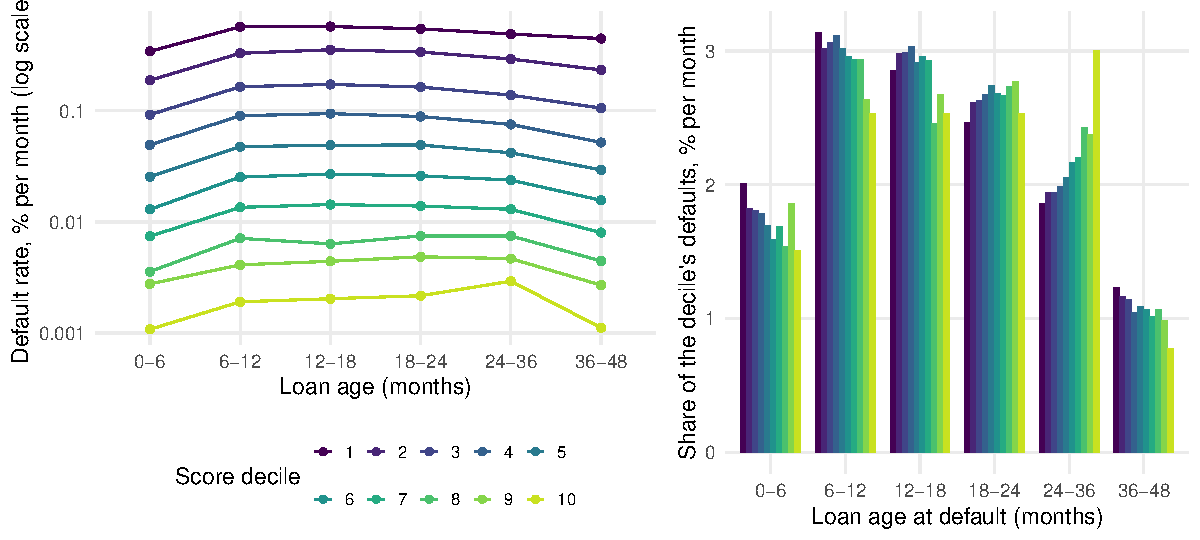
\includegraphics[width = \textwidth]{figures/fig_cdr_by_decile.pdf}
    \small Notes: Estimation sample. Left: defaults in the loan-age bin over loans at risk at the start of the bin, per month of bin width, by score decile (log scale). Right: the distribution of loan age at default within each decile, per month of bin width. The 48--96 month bin, with fewer than 300 loans at risk per decile, is omitted.
% replication: Code/exhibits/make_panel_figures.R, results/default_timing_by_group.csv
\end{figure}

\section{Replication of Every Exhibit}\label{appendix:replication}

Every table and figure in the paper is written by a script from the result files of the repository, and Table \ref{tab:replication_map} names the scripts and files for each; \texttt{Code/run\_local.sh} regenerates every exhibit from the committed results and \texttt{jobs/run\_all.sh} the results from the raw archives.

\begin{footnotesize}
% replication: Code/exhibits/make_replication_map.py; the replication comments inside every float of the draft
\begin{longtable}{@{}p{0.20\textwidth}p{0.30\textwidth}p{0.28\textwidth}p{0.20\textwidth}@{}}
\caption{Replication of every exhibit: generator scripts and result files}\label{tab:replication_map}\\
\toprule
Exhibit & Caption & Scripts (\texttt{Code/}) & Data (\texttt{results/}, \texttt{external/}) \\
\midrule
\endfirsthead
\toprule
Exhibit & Caption & Scripts & Data \\
\midrule
\endhead
\bottomrule
\endfoot
Table \ref{tab:nonclassical} & Non-classical preferences: the weight on a payment at date s, what the & -- & \texttt{a theory table}; \texttt{no data} \\
Table \ref{tab:mc_runoff_grid} & The structural model's hazard and payment elasticity by loan age, on a & \texttt{Code/local/mc\_runoff\_model\_grid.R, Code/exhibits/make\_mc\_tables.R} & -- \\
Table \ref{tab:mc_runoff_grid2} & The model calibrated to the default rate and to the level of the payme & \texttt{Code/local/mc\_runoff\_model\_grid2.R (stage MC2), Code/exhibits/make\_mc\_tables.R} & -- \\
Figure \ref{fig:runoff_profiles} & The payment margin over the life of the loan, 61--72 month contracts.  & \texttt{Code/type/T1i\_runoff\_panel.R, Code/local/mc\_runoff\_model\_grid.R, Code/exhibits/make\_runoff\_figures.R} & -- \\
Figure \ref{fig:runoff_shape} & The ratio of the payment elasticity at 48--60 months to the elasticity & \texttt{Code/exhibits/make\_runoff\_figures.R} & -- \\
Table \ref{tab:runoff_shape} & The decline of the payment elasticity by group at fixed contract lengt & \texttt{Code/local/runoff\_model\_inversion.R, Code/exhibits/make\_runoff\_figures.R} & -- \\
Table \ref{tab:persistent_extract} & The two calibrations of the stopping model beside the data: what each  & \texttt{Code/exhibits/make\_persistent\_tables.R} & -- \\
Table \ref{tab:rho_variance} & The variation in the discount rate, and in the other primitives, that  & \texttt{Code/local/mc\_rho\_variance.R} & -- \\
Figure \ref{fig:origination_volume} & Auto loans by origination cohort & \texttt{Code/exhibits/make\_panel\_figures.R} & \texttt{results/panel\_windows\_auto.csv} \\
Figure \ref{fig:design_map} & From designs to inputs to outputs. Left: each identification design an & -- & \texttt{Draft/figures/fig\_design\_map.tex (a diagram}; \texttt{no data)} \\
Figure \ref{fig:ds_pvalue} & The Dobbie--Song pair against the model on the grid of the annual rate & \texttt{Code/local/experiments\_ledger.R, Code/exhibits/make\_ds\_pvalue\_figure.R} & -- \\
Table \ref{tab:rho_within_states} & The rate from the within-borrower design, with the twelve largest stat & \texttt{Code/local/within\_reading.R} & -- \\
Figure \ref{fig:rho_within} & The rate by score decile, income quartile, age, origination period and & \texttt{Code/local/within\_reading.R} & -- \\
Table \ref{tab:liquidity} & Default as a portfolio choice, and the payment margin across local lab & \texttt{Code/extract/E3\_cross\_loan.R, Code/level/L3\_liquidity\_shocks.R, Code/exhibits/make\_summary\_tables.R} & -- \\
Figure \ref{fig:exposure_groups} & The payment margin across people, places and cohorts. Elasticity of ch & \texttt{Code/type/T1l\_windows\_panel.R, Code/exhibits/make\_exposure\_figures.R} & -- \\
Table \ref{tab:exposure} & The payment elasticity by group and exposure window & \texttt{Code/type/T1l\_windows\_panel.R, Code/exhibits/make\_exposure\_figures.R} & -- \\
Figure \ref{fig:exposure_geo} & Power-preserving splits. Left: the payment elasticity within 24 months & \texttt{Code/type/T1l\_windows\_panel.R, Code/exhibits/make\_exposure\_figures.R} & -- \\
Table \ref{tab:het_geo} & The population design beside the within-borrower design, by state and  & \texttt{Code/type/T1l\_windows\_panel.R, Code/local/heterogeneity\_population.R, Code/exhibits/make\_heterogeneity\_tables.R} & \texttt{results/heterogeneity\_population.csv} \\
Figure \ref{fig:het_agreement} & The population rate, raw and selection-adjusted, and the within-borrow & \texttt{Code/local/heterogeneity\_population.R, Code/exhibits/make\_heterogeneity\_tables.R} & \texttt{results/heterogeneity\_population.csv} \\
Figure \ref{fig:geo_politics} & The term-to-payment ratio and the payment elasticity by state against  & \texttt{Code/local/geo\_politics\_v2.R} & -- \\
Figure \ref{fig:geo_correlates} & Exposure (upper row) and the population rate (lower row) by state agai & \texttt{Code/local/geo\_correlates\_v3.R, Code/exhibits/make\_geo\_figures.R} & \texttt{results/geo\_correlates\_v3\_units.csv} \\
Table \ref{tab:comparison} & Discount Rate Estimates Across Studies & \texttt{Code/exhibits/make\_comparison\_table.R} & \texttt{results/rho\_within\_readings.csv, experiments\_rho\_summary.csv, panel\_windows\_auto.csv, prior\_estimates.csv} \\
Table \ref{tab:loan_summary} & The auto-loan analysis sample: quartiles of the key variables & \texttt{Code/exhibits/make\_summary\_tables.R} & \texttt{results/level\_summary\_stats.csv, results/panel\_summary\_stats.csv} \\
Figure \ref{fig:lambda_curve} & The present-payment premium as a function of the per-period default pr & \texttt{Code/local/lambda\_by\_default\_rate.R} & \texttt{results/lambda\_curve.csv, results/lambda\_by\_default\_rate.csv} \\
Table \ref{tab:mucorrection} & The marginal-utility ratio in the two-period calibration ( = 2) & \texttt{Code/local/mucorrection\_calibration.R (results/mucorrection\_table.csv), Code/exhibits/make\_mucorrection\_table.R} & -- \\
Table \ref{tab:ladder} & The correction ladder for the constant-weight estimate, applied cumula & \texttt{Code/level/L5\_ladder.R} & -- \\
Figure \ref{fig:cdr_by_decile} & Conditional default rate and loan age at default, by credit-score deci & \texttt{Code/exhibits/make\_panel\_figures.R, results/default\_timing\_by\_group.csv} & -- \\
Figure \ref{fig:rho_headline} & The rate. The within-borrower estimate of the annual discount rate by  & \texttt{Code/local/within\_reading.R, Code/exhibits/make\_rho\_headline\_figure.R} & -- \\
Table \ref{tab:summary_families} & Summary statistics by loan family & \texttt{Code/extract/E19\_summary\_stats.R, Code/exhibits/make\_table1.R} & -- \\
Figure \ref{fig:horizon_power} & The precision of the rate by horizon. Left: the standard error of the  & \texttt{Code/local/horizon\_power.R} & \texttt{results/horizon\_power.csv, results/rho\_within\_readings.csv} \\
Table \ref{tab:main_margins} & The two margins of default by exposure window & \texttt{Code/type/T1l\_windows\_panel.R, Code/identification/I6\_within\_person.R, Code/exhibits/make\_main\_table.R} & -- \\
Table \ref{tab:benchmark} & Published payment responses beside the bureau's, by margin & \texttt{Code/exhibits/make\_benchmark\_table.R} & \texttt{results/causal\_ledger\_literature.csv, identification\_within\_person.csv, identification\_within\_person\_by\_group\_logL.csv, spec\_search.csv, spec\_search\_v2.csv, panel\_windows\_auto.csv} \\
Table \ref{tab:rho_within} & The rate across people from the within-borrower design & \texttt{Code/identification/I6f\_within\_person\_by\_group.R, Code/identification/I6i\_within\_person\_by\_period.R, Code/local/within\_reading.R} & \texttt{results/rho\_within\_readings.csv, rho\_within\_tests.csv} \\
Table \ref{tab:term_by_score} & The term margin by credit-score decile and horizon (auto loans) & \texttt{Code/identification/I6c\_profile\_by\_decile\_full.R, Code/identification/I6b\_horizon\_profile\_by\_group.R, Code/exhibits/make\_term\_margin\_tables.py} & -- \\
Table \ref{tab:term_deficiency} & The early term effect where the balance cannot be pursued & \texttt{Code/identification/I3b\_deficiency\_powered.R, Code/exhibits/make\_term\_margin\_tables.py} & \texttt{external/state\_deficiency\_rules.csv} \\
Table \ref{tab:equity_margin} & The equity margin against the payment margin, first mortgages & \texttt{Code/extract/E15\_mortgage\_equity.R, Code/identification/I12\_equity\_margin.R, Code/exhibits/make\_equity\_table.R} & -- \\
Table \ref{tab:het_population} & The population design beside the within-borrower design, by group & \texttt{Code/type/T1l\_windows\_panel.R, Code/local/heterogeneity\_population.R, Code/exhibits/make\_heterogeneity\_tables.R} & \texttt{results/heterogeneity\_population.csv} \\
Table \ref{tab:geo_correlates} & What the geography of exposure, default and the population rate is cor & \texttt{Code/local/geo\_correlates\_v3.R, Code/exhibits/make\_geo\_figures.R} & \texttt{results/geo\_correlates\_v3.csv, geo\_correlates\_v3\_units.csv} \\
Table \ref{tab:person_place} & Person and place in auto-loan default: variance decomposition and move & \texttt{Code/identification/I7\_person\_place.R, Code/exhibits/make\_placeholder\_tables.R} & -- \\
Table \ref{tab:persistent_calibration} & The stopping model with i.i.d.\ and with persistent income: parameters & \texttt{Code/local/mc\_persistent\_model.R, Code/exhibits/make\_persistent\_tables.R} & \texttt{results/mc\_persistent\_calibration.csv, results/mc\_persistent\_iid\_limit.csv, results/mc\_within\_grid\_v3.csv} \\
Table \ref{tab:persistent_runoff} & The run-off of the payment elasticity: by discount rate and balance pe & \texttt{Code/local/mc\_persistent\_model.R, Code/exhibits/make\_persistent\_tables.R} & \texttt{results/mc\_persistent\_grid.csv, results/mc\_runoff\_model\_grid\_h0.22.csv, results/runoff\_model\_rho\_co\_h0.22.csv} \\
Table \ref{tab:persistent_windows} & The term-to-payment ratios R\_{12}, R\_{24} and R\_{36} by discount rate  & \texttt{Code/local/mc\_persistent\_model.R, Code/exhibits/make\_persistent\_tables.R} & \texttt{results/mc\_persistent\_grid.csv, results/mc\_within\_grid\_v3.csv, results/identification\_within\_person\_by\_group.csv} \\
Table \ref{tab:spec_search} & Candidate full-population specifications scored against the within-bor & \texttt{Code/identification/I6e\_spec\_search.R, Code/local/bridge\_spec\_score.R, Code/exhibits/make\_spec\_table.py} & -- \\
Table \ref{tab:loan_types} & The loan types as parallel laboratories & -- & \texttt{hand-written (Draft/tables/tab\_loan\_types.tex)}; \texttt{numbers checked against results/summary\_stats\_families.csv} \\
Table \ref{tab:data_four} & The four disclosures of the cited work for every exhibit type & -- & \texttt{hand-written from the cited survey}; \texttt{no data} \\
Table \ref{tab:within_by_group} & The term margin across and within borrower, by score decile & \texttt{Code/identification/I6f\_within\_person\_by\_group.R, Code/exhibits/make\_within\_group\_table.R} & -- \\
Table \ref{tab:bureau_ladder} & The across-borrower term margin adjusted for the penalty and selection & \texttt{Code/local/bureau\_rho\_ladder.R, Code/local/window\_formula.R, Code/exhibits/make\_ladder\_tables.R} & -- \\
Table \ref{tab:bureau_rho_groups} & The adjusted across-borrower ratio by group & \texttt{Code/local/bureau\_rho\_ladder.R, Code/exhibits/make\_ladder\_tables.R} & -- \\
Table \ref{tab:rho_place} & The within-borrower ratio by state across windows, and the rate at the & \texttt{Code/identification/I6f\_within\_person\_by\_group.R, Code/local/place\_windows.R} & \texttt{results/identification\_within\_person\_by\_group.csv, rho\_place\_windows.csv} \\
Table \ref{tab:place_timing} & The state's repossession and collection rules and the timing of the pe & \texttt{Code/local/place\_timing.R, Code/exhibits/make\_place\_timing\_table.R} & \texttt{results/place\_timing\_fit.csv, external/state\_repossession\_rules.csv} \\
Figure \ref{fig:rho_place_windows} & The window profile of the within-borrower ratio, twelve largest states & \texttt{Code/local/place\_windows.R} & \texttt{results/rho\_place\_windows.csv} \\
Table \ref{tab:rho_place_states} & The rate by state from place-by-score-tercile cells, twenty largest st & \texttt{Code/identification/I6h\_within\_person\_place\_cells.R, Code/local/place\_rates.R} & \texttt{results/identification\_within\_person\_place\_cells.csv, rho\_place.csv, rho\_place\_cells.csv} \\
Figure \ref{fig:rho_place} & The rate by place from place-by-score-tercile cells. Left: the twenty- & \texttt{Code/local/place\_rates.R} & \texttt{results/rho\_place.csv} \\
Table \ref{tab:experiments} & Rule-based experiments as payment-path treatments, and the model's est & \texttt{Code/local/experiments\_ledger.R, Code/exhibits/make\_experiments\_table.py} & \texttt{external/experiments\_paths.csv, external/experiments\_estimates.csv, results/experiments\_rho\_summary.csv} \\
Figure \ref{fig:rho_subgroups} & The discount rate by subgroup in the Dobbie--Song experiment. Each cur & \texttt{Code/local/experiments\_rho\_subgroups.R, Code/exhibits/make\_rho\_subgroups.R} & -- \\
Table \ref{tab:rho_subgroups} & The discount rate by subgroup in the Dobbie--Song experiment & \texttt{Code/local/experiments\_rho\_subgroups.R, Code/exhibits/make\_rho\_subgroups.R} & \texttt{results/experiments\_rho\_subgroups.csv} \\
Table \ref{tab:rho_posterior} & Posterior summaries of the rate under a flat prior, by pair and suppor & \texttt{Code/local/experiments\_rho\_posterior.R, Code/exhibits/make\_rho\_posterior\_table.R}; \texttt{results/experiments\_rho\_posterior.csv Code/local/experiments\_rho\_posterior.R, Code/exhibits/make\_rho\_posterior\_table.R} & \texttt{results/experiments\_rho\_posterior.csv} \\
Figure \ref{fig:ledger_paths} & Rule-based experiments as payment-path treatments & \texttt{Code/exhibits/make\_ledger\_figures.R} & \texttt{external/experiments\_paths.csv, external/experiments\_estimates.csv} \\
Figure \ref{fig:ledger_rho} & What each pair of arms says about the discount rate, and the near-hori & \texttt{Code/exhibits/make\_ledger\_figures.R, Code/exhibits/make\_lambda\_figure.R} & \texttt{results/experiments\_rho.csv, external/experiments\_estimates.csv} \\
Table \ref{tab:strategies} & Identification strategies for the discount rate: the record & \texttt{no generator, Code/local/geo\_rate\_regime.R} & \texttt{the record of the designs, written from the memos and results named in each row}; \texttt{results/geo\_rate\_regime.csv} \\
Table \ref{tab:identification} & The payment margin: fixed effects, instruments, and the corrected esti & \texttt{Code/identification/I2c\_margins\_iv.R, I2d\_difference\_estimator.R} & -- \\
Table \ref{tab:cards_probe} & Revolving trades in the archives: payment position, formula rate, and  & \texttt{Code/extract/E5\_cards\_probe.R, Code/exhibits/make\_placeholder\_tables.R} & \texttt{results/cards\_probe.csv} \\
Table \ref{tab:equity_groups} & The equity margin and the payment margin by score and income & \texttt{Code/identification/I12\_equity\_margin.R, Code/exhibits/make\_equity\_groups\_table.R} & \texttt{results/equity\_margin.csv} \\
Table \ref{tab:equity_bins} & The hazard by bin of the house-price change since origination & \texttt{Code/identification/I12\_equity\_margin.R, Code/exhibits/make\_equity\_groups\_table.R} & \texttt{results/equity\_margin\_bins.csv} \\
Table \ref{tab:equity_model} & The model's equity margin on a grid of discount rates & \texttt{Code/local/mc\_equity\_model.R, Code/exhibits/make\_equity\_table.R} & -- \\
Table \ref{tab:scf_questions} & Expectation and constraint questions in the 2022 Survey of Consumer Fi & \texttt{the survey questions and codes (Code/scf/scf\_beliefs.R uses them)} & \texttt{no data} \\
Table \ref{tab:scf_beliefs} & Beliefs in the Survey of Consumer Finances, by group & \texttt{Code/scf/scf\_beliefs.R} & \texttt{results/scf\_beliefs\_by\_group.csv} \\
Table \ref{tab:scf_beliefs_se} & Beliefs by group, with standard errors & \texttt{Code/scf/scf\_beliefs.R} & \texttt{results/scf\_beliefs\_by\_group.csv} \\
Table \ref{tab:scf_coholding} & The co-holding margin in the Survey of Consumer Finances, by group & \texttt{Code/scf/scf\_beliefs.R} & \texttt{results/scf\_coholding\_by\_group.csv} \\
Table \ref{tab:replication_map} & Replication of every exhibit: generator scripts and result files & -- & -- \\
\end{longtable}

\end{footnotesize}

\end{document}
